\documentclass[11pt, a4paper]{report}

% AA Lingua E Codifica
\usepackage[italian]{babel}
\usepackage[utf8]{inputenc}
\usepackage[T1]{fontenc}
\usepackage{lmodern}

% AA Layout Di Pagina E Tipografia
\usepackage[margin=2cm, top=1.5cm, bottom=1.5cm]{geometry}
\usepackage{parskip}
\usepackage[expansion=false]{microtype}

% AA Gestione Dei Colori
\usepackage{xcolor}

% AA Matematica E Simboli
\usepackage{amsmath, amssymb, amsfonts}
\usepackage{mathtools}
\usepackage{siunitx}

% BB OTTIMIZZAZIONE MATRICI LUNGHE PER LA STAMPA
\setlength{\arraycolsep}{10pt}
\usepackage{bm}

% AA Grafica, Immagini E Tabelle
\usepackage{graphicx}
\graphicspath{{./Images/Appunti}}
\usepackage{float}
\usepackage{booktabs}
\usepackage{array}
\usepackage{multirow}
\usepackage{tabularx}
\usepackage{arydshln}
\usepackage{listings}
\usepackage{tikz}
\usetikzlibrary{shapes.geometric, arrows.meta, positioning, calc, quotes}

% AA Link, Riferimenti Ed Elenchi
\usepackage[unicode]{hyperref}
\hypersetup{
    colorlinks=true,
    linkcolor=blue,
    urlcolor=blue,
    citecolor=blue,
    pdftitle={Capitolo 2},
    pdfauthor={Francesco Lo Verde},
    pdfpagemode=FullScreen,
}
\usepackage{bookmark}
\usepackage[italian,capitalize]{cleveref}
\usepackage{enumitem}
\setlist{noitemsep}

% AA Personalizzazione Titoli E Altri Pacchetti
\usepackage{titlesec}

% BB Formattazione Titoli
\titleformat{\chapter}[hang]{\normalfont\huge\bfseries}{\chaptername\ \thechapter:}{0.5em}{}
\titleformat{\section}{\normalfont\LARGE\bfseries}{\thesection}{0.8em}{}
\titleformat{\subsection}{\normalfont\Large\bfseries}{\thesubsection}{0.8em}{}
\titleformat{\subsubsection}{\normalfont\large\bfseries}{\thesubsubsection}{0.8em}{}

% BB Spaziatura Titoli
% CC Sintassi: \titlespacing*{livello}{sinistra}{spazio SOPRA}{spazio SOTTO}
\titlespacing*{\chapter}{0pt}{0pt}{6pt}
\titlespacing*{\section}{0pt}{10pt}{6pt}
\titlespacing*{\subsection}{0pt}{8pt}{6pt}
\titlespacing*{\subsubsection}{0pt}{6pt}{6pt}

\usepackage{comment}
\newtheorem{theorem}{Definizione}

\author{Francesco Lo Verde}
\begin{document}

% AA Riduzione Temporanea Margini Indice
% BB top=0.9cm bottom=1.6cm
% BB footskip=0.6cm (Garantisce Che Il Numero Di Pagina Non Sia Tagliato)
\newgeometry{margin=2cm, top=1cm, bottom=1.5cm, footskip=0.6cm}

{
  % BB Spazio Negativo Sopra Il Titolo Per Portare "Indice" Più In Alto
  \titlespacing*{\chapter}{0pt}{-25pt}{6pt}
  \tableofcontents
}

\addtocontents{toc}{\protect\vspace{-15pt}}
\restoregeometry
\newpage

\chapter{Introduzione}
\begin{theorem}
    \textbf{Robot Istitute Of America} (Libro)\\
    Un robot e una struttura meccanica multifunzionale e riprogrammabile progettato per spostare materiali, parti, utensili o dispositivi specializzati secondo movimenti variabili programmati per l’esecuzione di una varieta di compiti diversi.
\end{theorem}
\begin{figure}[h]
    \centering
    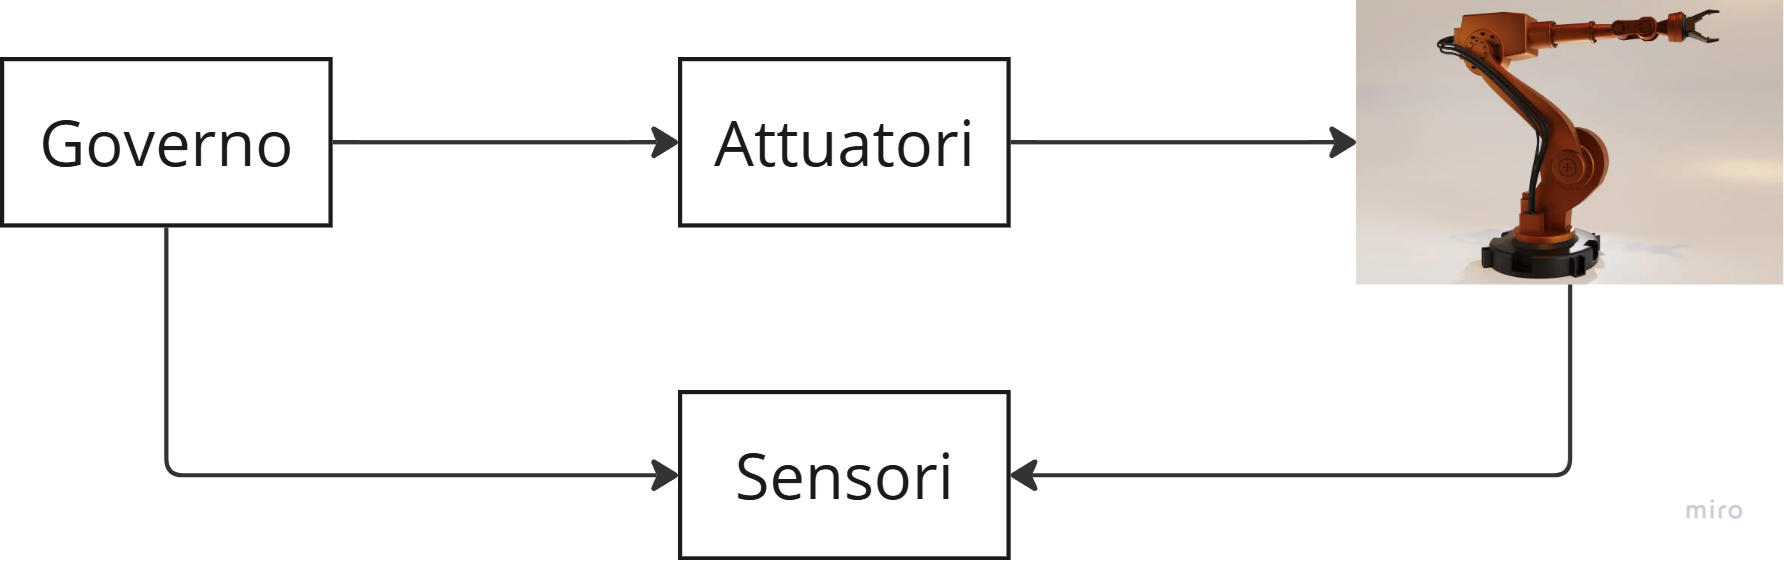
\includegraphics[width=0.5\linewidth]{Schema.png}
\end{figure}
Il movimento delle componenti meccaniche è generato da un \textbf{Sistema Di Attuazione}, costituito da servomotori e meccanismi di trasmissione. La percezione dell'ambiente è invece affidata a un \textbf{Sistema Sensoriale}, composto da sensori propriocettivi ed esterocettivi. Infine, un sistema di controllo elabora le informazioni disponibili e genera i comandi per il sistema di attuazione, consentendo al robot di muoversi e interagire con l'ambiente. Il sistema sensoriale permette inoltre di acquisire informazioni sullo stato interno del robot e sulle caratteristiche dell'ambiente circostante.
% AA Altre Definizioni
\begin{comment}
\begin{theorem}
    \textbf{ISO 8373}\\
    Un robot è un sistema meccanico programmabile, dotato di un certo grado di autonomia, capace di eseguire compiti fisici in ambienti strutturati o non strutturati.
\end{theorem}

\begin{theorem}
    \textbf{IFR}\\
    Un robot industriale è un manipolatore multifunzionale, programmabile in tre o più assi, capace di muoversi autonomamente per eseguire compiti specifici di manipolazione o assemblaggio.
\end{theorem}
\end{comment}

\section{Struttura Meccanica dei Robot}
I robot si distinguono in due categorie principali: \textbf{robot a base fissa}, detti manipolatori, e \textbf{robot mobili}.

\subsection{Robot A Base Fissa (Manipolatori)}
La struttura meccanica di un robot manipolatore consiste in un insieme di corpi ridigi (\textit{bracci}) interconnessi tra di loro per mezzo di articolazioni (\textit{giunti}); nel manipolatore si individuano una struttura portante, che ne assicura mobilità, un
\textit{polso}, che conferisce destrezza, e un \textit{organo terminale} che esegue il compito per cui il robot è utilizzato.\\
\textbf{La struttura fondamentale dei manipolatori è a catena cinematica aperta o seriale}

Dal punto di vista topologico, si distinguono:
\begin{itemize}
	\item \textbf{Catene Cinematiche Aperte}, in cui una sequenza unica di bracci collega gli estremi della catena.
	\item \textbf{Catene Cinematiche Chiuse}, in cui una sequenza di bracci forma un anello, riducendo i gradi di libertà a causa dei vincoli imposti.
\end{itemize}
La mobilità di un manipolatore `e assicurata dalla presenza dei giunti. L'articolazione tra due bracci consecutivi può essere realizzata con un giunto \textbf{prismatico} o \textbf{rotoidale}. Un giunto \textit{prismatico} permette traslazione tra due bracci, mentre un giunto \textit{rotoidale} consente la rotazione. La scelta tra queste soluzioni dipende da esigenze di compattezza e affidabilità.
In una catena cinematica aperta, ogni giunto (di entrambi i tipi) conferisce un singolo grado di libertà (DoF) e quindi questi dipendono dalla configurazione dei giunti.\\
I gradi di libertà devono essere opportunamente distribuiti lungo la struttura
meccanica in modo da essere in numero sufficiente per l'esecuzione di un dato
compito. Per operazioni tridimensionali, sono necessari almeno sei gradi di libertà (tre per la posizione e tre per l'orientamento). Un manipolatore con più DoF di quelli strettamente necessari è detto \textbf{ridondante}.\\
Lo \textit{spazio di lavoro} rappresenta la porzione dell'ambiente circostante a cui
può accedere l'organo terminale di un manipolatore. La sua forma e il suo volume
dipendono dalla struttura del manipolatore.
\newpage
\subsubsection{Tipologie di Manipolatori}
Il compito della \textit{struttura portante} è quello di posizionare il polso che orienterà l'organo terminale. Il tipo e la successione dei gradi di libertà della struttura portante, a partire dall'articolazione alla base, consente di classificare i manipolatori in:
\begin{itemize}
	\item \textbf{Manipolatori cartesiani}: Basati su tre giunti prismatici ortogonali, consentono movimenti rettilinei e alta precisione su tutto il volume di lavoro. Ad ogni grado di libertà corrispomde una variabile dello spazio cartesiano e quindi si possono immediatamente definire percorsi rettilinei. La precisione di posizionamento del polso è costante in tutto lo spazio. Lo spazio di lavoro è un parallelepipedo

	\item \textbf{Manipolatori cilindrici}: Presentano un giunto rotoidale alla base e due giunti prismatici. Descrivendo il compito in coordinate cilindriche ogni grado di libertà corrisponde ad una variabile dello spazio. La precisione di posizionamento del polso si riduce al crescere dello sbraccio orizzontale. Lo spazio di lavoro è una porzione di cilindro cavo

	\item \textbf{Manipolatori sferici}: con due giunti rotoidali (primo e secondo) e uno prismatico, permettono l'accesso a un ampio spazio di lavoro sferico, ma con minore rigidezza strutturale. Descrivendo il compito in coordinate sferiche ogni grado di libertà corrisponde ad una variabile dello spazio. La precisione di posizionamento del polso si riduce al crescere dello sbraccio radiale. Lo spazio di lavoro è una porzione di sfera cava


	\item \textbf{SCARA (Selective Compliance Assembly Robot Arm)}: Dotati di due giunti rotoidali e un prismatico, posizionati in modo tale che gli assi siano tutti paralleli tra di loro. Descrivendo il compito in coordinate cartesiane, la corrispondenza tra gradi di libertà e variabili dello spazio cartesiano è mantenuta solo per la componente verticale. La precisione di posizionamento del polso si riduce al crescere della distanza del polso dall'asse del primo giunto

	\item \textbf{Manipolatori antropomorfi}: Composti da tre giunti rotoidali (spalla, gomito e polso), simulano la mobilità del braccio umano, garantendo elevata destrezza. L'asse di rotazione del giunto di base è ortogonale agli altri due che sono paralleli tra loro. Si si perde del tutto la corrispondenza tra gradi di libertà e variabili dello spazio cartesiano, nonché la precisione di posizionamento del polso cambia in tutto lo spazio di lavoro

	\item \textbf{Manipolatori paralleli}: Caratterizzati da catene cinematiche chiuse, che connettono la base all'organo terminale. Il vantaggio è l'elevata rigidezza strutturale rispetto ai manipolatori a catena cinematica aperta
\end{itemize}

\subsubsection{Il Polso e l'Organo Terminale}
Per garantire orientamenti arbitrari in uno spazio tridimensionale, il polso deve possedere \textit{almeno tre gradi di libertà}, realizzati mediante giunti rotoidali. Questi giunti consentono movimenti indipendenti attorno a tre assi, permettendo al manipolatore di raggiungere qualsiasi orientamento desiderato. Tuttavia, poiché il polso costituisce la parte terminale del manipolatore, deve soddisfare requisiti di compattezza che spesso complicano il suo progetto meccanico.\\
La soluzione più efficace consiste è quella in cui i tre assi di rotazione si intersecano in un unico punto e questa configurazione è detta \textbf{Polso Sferico}. La caratteristica principale è il disaccoppiamento tra posizione e orientamento dell'organo terminale. In altre parole, la struttura portante del manipolatore è responsabile di posizionare il punto di intersezione degli assi del polso, mentre il polso stesso si occupa di determinare l'orientamento finale dell'organo terminale. Tale separazione semplifica notevolmente il coordinamento tra i movimenti della struttura portante e quelli del polso.\\
L'organo terminale di un manipolatore è scelto in base al compito specifico che il robot deve eseguire. Ad esempio, per compiti di trasporto, l'organo terminale è generalmente costituito da una pinza, per applicazioni di lavorazione o assemblaggio, invece, l'organo terminale può essere un utensile specializzato, come una torcia di saldatura, una fresa, un trapano o un avvitatore.

Un esempio pratico è rappresentato dai robot utilizzati nell'industria automobilistica, dove manipolatori dotati di torce di saldatura eseguono operazioni di giunzione su componenti metallici. In questo caso, la precisione del posizionamento e la capacità del polso di orientare correttamente la torcia sono fattori critici per garantire la qualità del risultato.

% La versatilità e la flessibilità dei robot manipolatori non devono indurre a pensare che tutte le strutture meccaniche siano equivalenti per l'esecuzione di un determinato compito. La scelta di un robot è infatti condizionata dall'applicazione specifica, che impone vincoli riguardanti:
% \begin{itemize}
%     \item \textbf{Dimensione e forma dello spazio di lavoro}: Il manipolatore deve essere in grado di raggiungere tutti i punti rilevanti per il compito.
%     \item \textbf{Portata di carico}: Il robot deve supportare il peso dell'organo terminale e dell'eventuale carico manipolato.
%     \item \textbf{Destrezza}: La capacità del polso di eseguire orientamenti complessi è essenziale per compiti che richiedono alta precisione.
%     \item \textbf{Precisione di posizionamento}: Errori minimi possono compromettere la qualità del risultato, soprattutto in applicazioni critiche come l'assemblaggio di componenti elettronici.
%     \item \textbf{Prestazioni dinamiche}: Velocità e accelerazione del manipolatore influenzano l'efficienza del processo produttivo.
% \end{itemize}

\newpage
\subsection{Robot Mobili}
I robot mobili sono caratterizzati dalla presenza di una base semovente che consente loro di spostarsi autonomamente nell'ambiente in cui operano. A differenza dei manipolatori, questi robot sono impiegati principalmente in applicazioni di servizio, dove un'elevata mobilità è un requisito essenziale. Da un punto di vista meccanico, un robot mobile è costituito da uno o più corpi rigidi dotati di un sistema di locomozione. In generale, si distinguono due categorie principali:


\begin{itemize}
    \item \textbf{Robot Mobili Su Ruote}: Questi robot presentano un corpo rigido (chassis) equipaggiato con ruote per la locomozione. In alcuni casi, possono essere collegati ad altri corpi rigidi (rimorchi) tramite giunti rotoidali, anch'essi dotati di ruote.
    \item \textbf{Robot Mobili Su Gambe}: Questa categoria include robot con più corpi rigidi connessi tra loro mediante giunti prismatici o rotoidali. Alcuni di questi corpi formano arti, le cui estremità (piedi) entrano periodicamente in contatto con il suolo per realizzare il movimento. La varietà di strutture è vasta e spesso si ispira alla biomeccanica degli organismi viventi (robotica biomimetica), spaziando dai robot bipedi umanoidi ai robot esapodi che emulano il movimento degli insetti.
\end{itemize}

Le ruote convenzionali si suddividono in tre categorie:
\begin{itemize}
    \item \textbf{Ruota Fissa}: ruota attorno a un asse passante per il suo centro e normale al piano, mantenendo un orientamento costante rispetto allo chassis.

    \item \textbf{Ruota Orientabile}: presenta due assi di rotazione: uno uguale a quello della ruota fissa per la rotazione e uno verticale che ne consente l'orientamento rispetto allo chassis.

    \item \textbf{Ruota Eccentrica (Caster)}: simile alla ruota orientabile, ma con l'asse verticale spostato rispetto al centro della ruota. Questa configurazione permette alla ruota di allinearsi automaticamente alla direzione di spostamento dello chassis, senza influenzarne la mobilità.
\end{itemize}

I robot mobili possono adottare diverse configurazioni di trazione, tra cui:
\begin{itemize}
    \item \textbf{Trazione Differenziale}: Questa configurazione prevede due ruote fisse con un asse di rotazione comune e una o più ruote eccentriche per il bilanciamento statico. Il robot può ruotare sul posto se le velocità angolari delle due ruote principali sono uguali e opposte.

    \item \textbf{Trazione Sincronizzata}: Un robot con questa configurazione possiede tre ruote orientabili allineate, controllate da due motori: uno per la trazione e uno per l'orientamento.

    \item \textbf{Configurazione Triciclo}: Comprende due ruote fisse posteriori e una ruota orientabile anteriore. La trazione è fornita da un unico motore per le ruote fisse, mentre un secondo motore controlla l'orientamento della ruota anteriore e quindi agisce da sterzo.

    \item \textbf{Configurazione Automobilistica}: Presenta due ruote fisse posteriori e due ruote orientabili anteriori. Un motore fornisce la trazione, mentre un altro gestisce l'orientamento delle ruote anteriori. Per evitare slittamenti in curva, le ruote anteriori assumono angoli di sterzata differenti: la ruota interna è più sterzata rispetto a quella esterna. A differenza dei precedenti, questo veicolo è \textit{omnidirezionale}, cioè può muoversi istantaneamente in qualsiasi direzione
\end{itemize}

% Oltre alle ruote convenzionali, esistono ruote speciali come la \textbf{ruota Mecanum} (o svedese), dotata di rulli passivi inclinati (solitamente di $45^{\circ}$), che permettono una mobilità omnidirezionale.

\subsubsection{Bilanciamento e Stabilità}
Nel caso dei robot mobili su ruote, il bilanciamento non costituisce generalmente un problema. Un robot con tre ruote è in equilibrio statico se il baricentro si trova all'interno del triangolo di supporto formato dai punti di contatto delle ruote con il suolo. Nei robot con più di tre ruote, il poligono di supporto garantisce maggiore stabilità, ma in presenza di superfici irregolari è necessario un sistema di sospensioni per mantenere il contatto con il suolo.\\
A differenza dei manipolatori, lo spazio di lavoro di un robot mobile può essere potenzialmente illimitato. Tuttavia, un robot non omnidirezionale presenta restrizioni sui moti istantanei ammissibili. Ad esempio, un robot a triciclo non può muoversi immediatamente in direzione perpendicolare all'asse delle ruote posteriori, sebbene sia comunque in grado di raggiungere tale posizione attraverso manovre appropriate. In generale, le limitazioni istantanee non precludono la possibilità di raggiungere qualsiasi posizione e orientamento all'interno dello spazio di lavoro.

\newpage
\subsection{Robotica Industriale}

La robotica industriale si occupa della progettazione, del controllo e delle applicazioni dei robot in ambito produttivo. I robot industriali operano in ambienti strutturati, le cui caratteristiche geometriche e fisiche sono note a priori. Grazie agli sviluppi tecnologici, questa disciplina ha raggiunto un alto grado di maturità, diventando un pilastro dell'automazione moderna.

L'automazione industriale ha l'obiettivo di sostituire l'uomo in un processo produttivo, non solo nell'esecuzione delle operazioni materiali, ma anche nell'elaborazione intelligente delle informazioni sullo stato del processo. A seconda della flessibilità del sistema, si distinguono tre principali tipologie di automazione:

\begin{itemize}
    \item \textbf{Automazione Rigida}: Impiegata in contesti produttivi caratterizzati da elevati volumi di produzione di manufatti con caratteristiche costanti. In questi scenari, la necessità di garantire alta produttività e qualità impone l'uso di macchinari specializzati e sequenze operative prestabilite. Questo tipo di automazione è tipico delle catene di montaggio, in cui la ripetitività e l'efficienza sono prioritarie.
    \item \textbf{Automazione Programmabile}: Adottata in ambienti di produzione orientati alla realizzazione di piccoli e medi lotti di prodotti con caratteristiche variabili. Un sistema di automazione programmabile consente di modificare le sequenze operative attraverso la riprogrammazione dei macchinari, permettendo una maggiore adattabilità alle esigenze produttive. Questo approccio è tipico di industrie che devono rispondere a una domanda diversificata, come quelle del settore automobilistico e dell'elettronica.
    \item \textbf{Automazione Flessibile}: Rappresenta l'evoluzione dell'automazione programmabile, consentendo la produzione di lotti variabili con un'efficienza superiore. Il suo obiettivo è minimizzare i tempi di inattività necessari per la riprogrammazione delle operazioni e delle macchine impiegate. Tale automazione si basa su sistemi di controllo avanzati e robot industriali dotati di sensori e algoritmi di apprendimento automatico, che li rendono in grado di adattarsi dinamicamente alle variazioni della produzione.
\end{itemize}

Un robot industriale possiede tre capacità fondamentali che lo rendono essenziale nei processi manifatturieri:

\begin{itemize}
    \item \textbf{Trasporto}: Movimentazione di componenti e prodotti all'interno della
    linea di produzione;
    \item \textbf{Manipolazione}: Esecuzione di operazioni di assemblaggio, saldatura, verniciatura e altre attività che richiedono precisione;
    \item \textbf{Misura}: Acquisizione di dati relativi alla qualità del prodotto e alle condizioni operative, permettendo il controllo e l'ottimizzazione del processo.
\end{itemize}
\newpage
\section{Modellistica, Pianificazione, E Controllo Di Robot}
In tutte le applicazioni robotiche, l'esecuzione di un compito richiede l'implementazione di un movimento pianificato. La corretta realizzazione di tale movimento dipende dall'unità di governo, la quale fornisce i comandi necessari agli attuatori del robot. Per garantire un'esecuzione precisa, è essenziale un'analisi approfondita della struttura meccanica, degli attuatori e dei sensori.
L'obiettivo di questa analisi è la derivazione di modelli matematici capaci di descrivere i legami tra i vari componenti del robot, fornendo così una base indispensabile per la progettazione delle strategie di controllo del movimento.

\subsection{Modellistica}
L'analisi cinematica di un robot si occupa della descrizione del moto rispetto a un sistema di riferimento cartesiano fisso, senza considerare le forze e i momenti che lo generano.
Essa si distingue in cinematica diretta e inversa:
\begin{itemize}
    \item \textbf{Cinematica Diretta}: Determina la posizione e l'orientamento dell'organo terminale a partire dalle coordinate dei giunti.
    \item \textbf{Cinematica Inversa}: Consente di calcolare i moti dei giunti necessari per raggiungere una specifica posizione e orientamento dell'organo terminale.
\end{itemize}

La cinematica differenziale, tramite lo Jacobiano del manipolatore, descrive le relazioni tra le velocità dei giunti e quelle dell'organo terminale. Essa costituisce la base per derivare il modello dinamico del robot, che esprime le equazioni del moto in funzione delle forze e dei momenti applicati. Un modello dinamico accurato è essenziale per dimensionare gli attuatori, progettare strategie di controllo e simulare il comportamento del sistema.
\begin{comment}
Nel caso dei robot mobili, la modellistica si differenzia da quella dei manipolatori per la presenza di vincoli cinematici legati alle ruote. Tali vincoli, integrabili o meno a seconda della struttura meccanica, influenzano direttamente la mobilità del robot. Il modello cinematico descrive i moti istantanei ammissibili sotto tali vincoli, mentre il modello dinamico, che include le reazioni vincolari, lega questi moti alle forze generalizzate agenti sul sistema.
\end{comment}
\subsection{Pianificazione Del Movimento}
La pianificazione del moto definisce il movimento da imporre ai giunti o direttamente all'organo terminale. Si distinguono due principali approcci:
\begin{itemize}
    \item \textbf{Moto Punto-Punto}: Utilizzato in operazioni di trasporto, in cui è sufficiente definire le posizioni di partenza e di arrivo.
    \item \textbf{Moto Su Percorso Assegnato}: Impiegato in lavorazioni, dove l'organo terminale deve seguire una traiettoria specifica.
\end{itemize}
Il problema di pianificazione nei robot mobili consiste nel generare traiettorie che conducano il veicolo da una configurazione iniziale a una finale. Se lo spazio di lavoro contiene ostacoli, la pianificazione deve garantire l'assenza di collisioni.Tale problema, noto come \textit{pianificazione del moto}, si può formulare in modo valido tanto per i manipolatori quanto per i robot mobili utilizzando il concetto di spazio delle configurazioni.

\subsection{Controllo del Movimento}
Il controllo di un robot richiede l'uso di attuatori e sensori per garantire l'esecuzione delle traiettorie pianificate, che costituiscono gli ingressi di riferimento per il sistema di controllo. Il problema principale nel controllo di un manipolatore è determinare le forze e le coppie che gli attuatori devono applicare ai giunti per seguire tali traiettorie. Questo compito è complesso poiché i manipolatori sono sistemi articolati in cui il moto di un braccio influenza quello degli altri. Le equazioni del moto evidenziano, tranne nel caso di strutture cartesiane ad assi ortogonali, accoppiamenti dinamici tra i giunti. La sintesi delle forze e coppie non può basarsi solo sul modello dinamico, poiché esso non descrive completamente la struttura reale. Pertanto, il controllo si affida alla retroazione: valutando lo scostamento tra i riferimenti e le misure dei sensori propriocettivi, un sistema in retroazione soddisfa le specifiche di precisione richieste.

Il controllo di un robot mobile differisce sostanzialmente da quello dei manipolatori. In questo caso, il numero di ingressi di controllo è sempre inferiore al numero di variabili di configurazione. Di conseguenza, la struttura di un controllore per l'inseguimento di traiettorie è necessariamente diversa da quella di un controllore per raggiungere una configurazione specifica.

% AA Capitolo 2

\chapter{Cineamatica}
\section{Posa di un Corpo Rigido}
La \textbf{posa} di un corpo rigido descrive la sua \textbf{posizione} e il suo \textbf{orientamento} rispetto a una terna di riferimento.

Prendendo come riferimento il sistema di coordinate $ RF_A $
\begin{center}
    \begin{tikzpicture}
        % Disegna gli assi
        \draw[->] (0,0,0) -- (2,0,0) node[anchor=north east] {\textbf{x}};
        \draw[->] (0,0,0) -- (0,2,0) node[anchor=north west] {\textbf{y}};
        \draw[->] (0,0,0) -- (0,0,2) node[anchor=south] {\textbf{z}};

        \filldraw[black] (0,0,0) circle (1.5pt) node[anchor=south east] {${A}$};
        \filldraw[black] (2,2,2) circle (1.5pt) node[anchor=south east] {${B}$};
    \end{tikzpicture}
\end{center}
La posizione del punto $ B $ rispetto al sistema di riferimento $ RF_{A} $ può essere rappresentata tramite le coordinate cartesiane $ x_{A}, y_{A}, z_{A} $. Queste coordinate sono espresse rispetto alla terna di assi $ \mathbf{x}_A, \mathbf{y}_A, \mathbf{z}_A $, con origine nel punto $ A $, che è l'origine di $ RF_{A} $.

Il vettore $ ^{A}\mathbf{p}_{AB} $ rappresenta lo spostamento necessario per andare dall'origine $ A $ del sistema di riferimento $ RF_{A} $ al punto $ B $.

\fbox{Questo vettore descrive la posizione del punto $ B $ rispetto al sistema di riferimento $ RF_A $.}

Tale vettore è espresso come:

$$
^{A}\mathbf{p}_{AB} =
\begin{bmatrix}
x_A \\
y_A \\
z_A
\end{bmatrix},
$$

Dove, $ x_{A} $, $ y_{A} $, $ z_{A} $ sono le componenti (coordinate) del vettore lungo gli assi $ \mathbf{x}_A $, $ \mathbf{y}_A $, $ \mathbf{z}_A $, rispettivamente.

Questo vettore è un \textit{vettore applicato}, poiché descrive lo spostamento necessario per andare dall'origine di $ RF_A $ al punto $ B $. In altre parole, sono specificati
\begin{itemize}
    \item Il \textbf{Punto Di Applicazione} di $^{A}\mathbf{p}_{AB}$ che è l'origine di RFA
    \item La \textbf{Direzione} e il \textbf{Modulo} di $^{A}\mathbf{p}_{AB}$ che indicano rispettivamente la direzione e la distanza tra l'origine di $ RF_A $ e il punto $ B $
\end{itemize}

Per caratterizzare l'\textbf{orientamento} del corpo rigido, si introduce un secondo riferimento $ RF_B $ solidale al corpo rigido e avente origine in $ B $ e siano $ \mathbf{x}_B, \mathbf{y}_B, \mathbf{z}_B $ i versori degli assi di $ RF_B $.
\begin{center}
    \begin{tikzpicture}
        % Disegna gli assi
        \draw[->] (0,0,0) -- (3,0,0) node[anchor=north east] {\textbf{x}};
        \draw[->] (0,0,0) -- (0,3,0) node[anchor=north west] {\textbf{y}};
        \draw[->] (0,0,0) -- (0,0,3) node[anchor=south] {\textbf{z}};

        \filldraw[black] (0,0,0) circle (1.5pt) node[anchor=south east] {${A}$};
        \filldraw[black] (2,2,2) circle (1.5pt) node[anchor=south east] {${B}$};

        % Nuovo sistema di riferimento con origine in B
        \begin{scope}[shift={(2,2,2)}]
            % Disegna i nuovi assi con orientamento diverso
            \draw[red,->] (0,0,0) -- (1,0.5,0) node[anchor=north east] {\textbf{x'}};
            \draw[red,->] (0,0,0) -- (-0.5,1,0) node[anchor=north west] {\textbf{y'}};
            \draw[red,->] (0,0,0) -- (0,-0.5,1) node[anchor=south] {\textbf{z'}};
        \end{scope}
    \end{tikzpicture}
\end{center}

Si può indicare la posizione di un punto del corpo rigido rispetto al riferimento solidale tramite il vettore espresso come
$$
    ^{B}\mathbf{p} =
    \begin{bmatrix}
    x_B \\
    y_B \\
    z_B
    \end{bmatrix},
$$
\newpage
\subsection{Matrice Di Rotazione}
% $^{0}\mathbf{R}_{1}$ la matrice che uso per trasformare una terna espressa nelle coordinate $\mathbf{RF_{0}}$ in una terna espressa in coordinate della terna di $\mathbf{RF_{1}}$
Per descrivere l'orientamento di $ RF_{B} $ rispetto a $ RF_{A} $, si considerano i versori degli assi di $ RF_{B} $ ($ \mathbf{x}_{B}, \mathbf{y}_{B}, \mathbf{z}_{B} $) e si esprimono come combinazione lineari dei versori degli assi di $ RF_{A} $ ($ \mathbf{x}_{A}, \mathbf{y}_{A}, \mathbf{z}_{A} $)\\
% Versori Di RFA
% i_{A} = [1 0 0]       j_{A} = [0 1 0]       k_{A} = [0 0 1]
% Versore X             Versore Y             Versore Z
Si avrà quindi
\[
    \begin{cases}
        \mathbf{x}_B = x_{B_x} \mathbf{x}_A + x_{B_y} \mathbf{y}_A + x_{B_z} \mathbf{z}_A\\
        \mathbf{y}_B = y_{B_x} \mathbf{x}_A + y_{B_y} \mathbf{y}_A + y_{B_z} \mathbf{z}_A\\
        \mathbf{z}_B = z_{B_x} \mathbf{x}_A + z_{B_y} \mathbf{y}_A + z_{B_z} \mathbf{z}_A
    \end{cases}
\]
Dove:
\begin{itemize}
    \item $\mathbf{x}_A, \mathbf{y}_A, \mathbf{z}_A$ sono i versori, rispettivamente, dell'asse $x_{A}$, dell'asse $y_{A}$ e dell'asse $z_{A}$ di RFA
    \item $x_{B_x}$, $x_{B_y}$, $x_{B_z}$ sono le componenti del versore di $x_{B}$ rispetto alla base RFA (Incognite)
    \item $y_{B_x}$, $y_{B_y}$, $z_{B_z}$ sono le componenti del versore di $y_{B}$ rispetto alla base RFA (Incognite)
    \item $z_{B_x}$, $z_{B_y}$, $z_{B_z}$ sono le componenti del versore di $x_{B}$ rispetto alla base RFA (Incognite)
\end{itemize}
Utilizzando una notazione compatta, i tre versori che esprimono l'orientamento del corpo rispetto alla terna di riferimento ($RF_{A}$) possono essere combinati in una matrice
\[
    R =
    \begin{bmatrix}
        x_{B_x} & x_{B_y} & x_{B_z}\\
        y_{B_x} & y_{B_y} & y_{B_z} \\
        z_{B_x} & z_{B_y} & z_{B_z}
    \end{bmatrix}
\]
Le componenti dei versori di $ RF_B $ rispetto alla base di $ RF_A $ possono essere calcolate usando il prodotto scalare.\\
Quindi, ad esempio:
\[
    x_{B_x} = \mathbf{x}_B \cdot \mathbf{x}_A = x_{B_{x}}x_{A_{x}} + x_{B_{y}}x_{A_{y}} + x_{B_{z}}x_{A_{z}}
\]
Lo stesso ragionamento si applica a tutte le componenti e ai versori $ \mathbf{y}_B $ e $ \mathbf{z}_B $\\
Si nota che
\[
    x_{B_{x}}x_{A_{x}} + x_{B_{y}}x_{A_{y}} + x_{B_{z}}x_{A_{z}} = \mathbf{x}_B^{T}\mathbf{x}_A
\]
La relazione precedente, in forma matriciale, è detta \textbf{Matrice di Rotazione} ed è definita come:
\[
    \mathbf{R} =
    \begin{bmatrix}
        \mathbf{x}_B^{T}\mathbf{x}_A & \mathbf{y}_B^{T}\mathbf{x}_A & \mathbf{z}_B^{T}\mathbf{x}_A\\
        \mathbf{x}_B^{T}\mathbf{y}_A & \mathbf{y}_B^{T}\mathbf{y}_A & \mathbf{z}_B^{T}\mathbf{y}_A\\
        \mathbf{x}_B^{T}\mathbf{z}_A & \mathbf{y}_B^{T}\mathbf{z}_A & \mathbf{z}_B^{T}\mathbf{z}_A
    \end{bmatrix}
    =
    \begin{bmatrix}
        ^{A}\mathbf{x}_{B} & ^{A}\mathbf{y}_{B} & ^{A}\mathbf{z}_{B}
    \end{bmatrix}
\]
Dove ciascun \textit{vettore colonna} rappresenta i \textbf{coseni direttori} degli assi di \(RF_{B}\) nelle coordinate di \(RF_{A}\)
\subsubsection{Proprietà Matrice Di Rotazione}
È significativo notare che i vettori colonna della matrice \textbf{R} essendo rappresentativi di una terna ortonormale, sono ortogonali tra di loro:
\[
    \mathbf{x}_{B}^{T} \; \mathbf{y}_{B} = 0 \qquad \mathbf{y}_{B}^{T} \; \mathbf{z}_{B} = 0 \qquad \mathbf{z}_{B}^{T} \; \mathbf{x}_{B} = 0
\]
Inoltre, hanno modulo unitario:
\[
    \mathbf{x}_{B}^{T} \; \mathbf{x}_{B} = 1 \qquad \mathbf{y}_{B}^{T} \; \mathbf{y}_{B} = 1 \qquad \mathbf{z}_{B}^{T} \; \mathbf{z}_{B} = 1
\]
La matrice di rotazione R risulta \textit{ortogonale}, ovvero
\[
    \mathbf{R}^{T}\mathbf{R} = \mathbf{I}_{3}
\]
Dove $\mathbf{I}_{3}$ è la matrice di identità $3 \times 3$

Moltiplicando per $\mathbf{R}^{-1}$ da destra ambo i membri la precedente si ottiene che
\[
    \mathbf{R}^{T} = \mathbf{R}^{-1}
\]
Inoltre
\[
    \det(\mathbf{R}) = 1
\]
Quindi, si può dire che la matrice di rotazione appartiene al \textbf{\textit{Gruppo Speciale Ortonormale}} $SO(m)$ delle matrici reali $ m \times m$ con colonne ortonormali e determinante pari a 1
\newpage
\subsubsection{Rotazioni Elementari}

Consideriamo una rotazione elementare partendo da un sistema di riferimento $ RF_A $, caratterizzato dalla terna cartesiana $ O\text{-}xyz $. Supponiamo di ruotare il sistema di un angolo $\alpha$ intorno all'asse $z$, ottenendo una nuova terna $ O\text{-}x'y'z' $.

\begin{center}
    \begin{tikzpicture}
        % Disegna gli assi
        \draw[->] (0,0,0) -- (2,0,0) node[anchor=north east] {\textbf{x}};
        \draw[->] (0,0,0) -- (0,2,0) node[anchor=north west] {\textbf{y}};
        \draw[->] (0,0,0) -- (0,0,2) node[anchor=south] {\textbf{z}};
    \end{tikzpicture}
    \qquad\qquad
    \begin{tikzpicture}
        % Disegna gli assi ruotati di 60° attorno a z
        \begin{scope}[rotate around={70:(0,0,1)}]
            \draw[blue, ->] (0,0,0) -- (2,0,0) node[anchor=north east] {\textbf{x'}};
            \draw[blue, ->] (0,0,0) -- (0,2,0) node[anchor=north west] {\textbf{y'}};
            \draw[blue, ->] (0,0,0) -- (0,0,2) node[anchor=south] {\textbf{z'}};
        \end{scope}
    \end{tikzpicture}
\end{center}

Gli assi della nuova terna possono essere espressi in termini delle loro componenti rispetto alla terna originale. I versori degli assi della nuova terna sono dati da:
\[
\mathbf{x}' =
\begin{bmatrix}
    \cos(\alpha) \\
    \sin(\alpha) \\
    0
\end{bmatrix},
\qquad
\mathbf{y}' =
\begin{bmatrix}
    -\sin(\alpha) \\
    \cos(\alpha) \\
    0
\end{bmatrix},
\qquad
\mathbf{z}' =
\begin{bmatrix}
    0 \\
    0 \\
    1
\end{bmatrix}.
\]

Questi versori rappresentano le direzioni degli assi $x'$, $y'$ e $z'$ rispetto alla terna originale. La matrice di rotazione associata a questa trasformazione è costruita disponendo i versori come colonne:
\[
\mathbf{R}_{z}(\alpha) =
\begin{bmatrix}
    \cos(\alpha) & -\sin(\alpha) & 0 \\
    \sin(\alpha) & \cos(\alpha) & 0 \\
    0 & 0 & 1
\end{bmatrix}.
\]

Questa matrice descrive completamente la rotazione intorno all'asse $z$. In modo analogo, possiamo definire le matrici di rotazione per rotazioni intorno agli altri due assi coordinati. Per una rotazione di un angolo $\beta$ intorno all'asse $y$ e per una rotazione di un angolo $\gamma$ intorno all'asse $x$, le matrici saranno
\[
\mathbf{R}_{y}(\beta) =
\begin{bmatrix}
    \cos(\beta) & 0 & \sin(\beta) \\
    0 & 1 & 0 \\
    -\sin(\beta) & 0 & \cos(\beta)
\end{bmatrix}
\qquad\qquad
\mathbf{R}_{X}(\gamma) =
\begin{bmatrix}
    1 & 0 & 0 \\
    0 & \cos(\gamma) & -\sin(\gamma) \\
    0 & \sin(\gamma) & \cos(\gamma)
\end{bmatrix}
\]

Le matrici di rotazione godono di una proprietà importante: la matrice che descrive una rotazione di un angolo $-\theta$ intorno a un asse $K$ è uguale alla trasposta della matrice che descrive una rotazione di un angolo $\theta$ intorno allo stesso asse. In formule:
\[
\mathbf{R}_{K}(-\theta) = \mathbf{R}_{K}^{T}(\theta).
\]

Questa proprietà riflette il fatto che invertire la direzione di rotazione equivale a considerare l'inversa della trasformazione, che per matrici ortogonali coincide con la trasposta.
\subsubsection{Chain Rule}
Le matrici di rotazione seguono la cosiddetta \emph{Chain Rule}, che consente di comporre rotazioni successive. Se si hanno due sistemi di riferimento intermedi, \( RF_{B} \) e \( RF_{C} \), e si vuole esprimere l'orientamento di \( RF_{C} \) rispetto a \( RF_{A} \), si può scrivere:

\[
^{A}\mathbf{R}_{B} \cdot ^{B}\mathbf{R}_{C} = ^{A}\mathbf{R}_{C}
\]

In altre parole, la rotazione complessiva da \( RF_{A} \) a \( RF_{C} \) si ottiene moltiplicando la matrice di rotazione da \( RF_{A} \) a \( RF_{B} \) per quella da \( RF_{B} \) a \( RF_{C} \). Questa proprietà evidenzia come le rotazioni possano essere concatenate in modo sequenziale.
\newpage
\subsubsection{Cambiamento Di Coordinate}
Una matrice di rotazione può essere utilizzata per esprimere un cambiamento di coordinate tra due sistemi di riferimento. Supponiamo di avere un punto $ P $ espresso nel sistema di riferimento $ RF_{1} $ come $ ^1\mathbf{P} = [^1P_x, ^1P_y, ^1P_z]^T $. Per esprimere le coordinate di $ P $ nel sistema di riferimento $ RF_{0} $, utilizziamo la matrice di rotazione $ ^{0}\mathbf{R}_{1} $, che rappresenta l'orientamento di $ RF_{1} $ rispetto a $ RF_{0} $. Il cambiamento di coordinate è dato da:
\[
    ^0\mathbf{P} \; = \; ^{0}\mathbf{R}_{1} \; \cdot \;^{1}\mathbf{P}.
\]
Qui, $ ^{0}\mathbf{R}_{1} $ agisce come operatore di trasformazione delle coordinate dal sistema $ RF_{1} $ al sistema $ RF_{0} $.

\subsubsection{Rappresentazioni della Matrice di Rotazione}

La matrice di rotazione $\mathbf{R}$ è uno strumento fondamentale per descrivere trasformazioni rigide nello spazio tridimensionale. Essa può essere utilizzata in diversi contesti, ognuno dei quali evidenzia una specifica interpretazione della sua funzione:

\begin{enumerate}
    \item \textbf{Descrizione dell'Orientamento di un Corpo Rigido} \\
    La matrice di rotazione può rappresentare l'orientamento di un sistema di riferimento solidale a un corpo rigido rispetto a un sistema di riferimento fisso. Ad esempio, se consideriamo un sistema di riferimento $1$ ruotato rispetto al sistema di riferimento $0$, i versori degli assi di $1$ espressi nel sistema $0$ possono essere descritti come:
    \[
    \begin{bmatrix}
    ^{0}x_{1} \\
    ^{0}y_{1} \\
    ^{0}z_{1}
    \end{bmatrix}
    = \mathbf{R}_{Z}(\theta),
    \]
    dove $\mathbf{R}_{Z}(\theta)$ rappresenta una rotazione attorno all'asse $Z$ di un angolo $\theta$.

    \item \textbf{Trasformazione di Coordinate} \\
    La matrice di rotazione permette di convertire le coordinate di un punto da un sistema di riferimento a un altro. Se $^{1}P$ rappresenta le coordinate di un punto $P$ nel sistema di riferimento $1$, le sue coordinate nel sistema di riferimento $0$ possono essere ottenute mediante la relazione:
    \[
    ^{0}P = \mathbf{R}_{Z}(\theta) \cdot ^{1}P.
    \]

    \item \textbf{Applicazione di una Rotazione a un Vettore} \\
    Infine, la matrice di rotazione può essere utilizzata per ruotare un vettore $v$ nello spazio. Dato un vettore $v$ espresso in un sistema di riferimento, il vettore ruotato $v'$ si ottiene come:
    \[
    v' = \mathbf{R}_{Z}(\theta) \cdot v.
    \]
\end{enumerate}

In sintesi, la matrice di rotazione $\mathbf{R}$ è uno strumento versatile che consente di descrivere orientamenti, effettuare cambiamenti di coordinate e applicare trasformazioni geometriche, rendendola indispensabile in ambiti come la robotica, la meccanica e la grafica computazionale.
\subsubsection{Conclusioni}
\noindent
\begin{minipage}{0.5\textwidth}
    \begin{tikzpicture}
        % Disegna gli assi
        \draw[->] (0,0,0) -- (4,0,0) node[anchor=north east] {$\mathbf{x_{A}}$};
        \draw[->] (0,0,0) -- (0,4,0) node[anchor=north west] {$\mathbf{y_{A}}$};
        \draw[->] (0,0,0) -- (0,0,4) node[anchor=south] {$\mathbf{z_{A}}$};

        \filldraw[black] (0,0,0) circle (1.5pt) node[anchor=south east] {${A}$};
        \filldraw[black] (3,3,3) circle (1.5pt) node[anchor=south east] {${B}$};

        % Nuovo sistema di riferimento con origine in B
        \begin{scope}[shift={(3,3,3)}]
            % Disegna i nuovi assi con orientamento diverso
            \draw[red,->] (0,0,0) -- (2,0,0) node[anchor=north east] {$\mathbf{x_{B}}$};
            \draw[red,->] (0,0,0) -- (0,2,0) node[anchor=north west] {$\mathbf{y_{B}}$};
            \draw[red,->] (0,0,0) -- (0,0,2) node[anchor=south] {$\mathbf{z_{B}}$};

            \filldraw[blue,opacity=0.3]
                (1,0,1.5) -- (1,0.5,0) -- (0.5,1.5,1) -- (-0.5,1,1.5) -- cycle;
        \end{scope}
    \end{tikzpicture}
\end{minipage}
\hfill
\begin{minipage}{0.5\textwidth}
Avendo
\begin{enumerate}
    % Posizione del punto B rispetto al sistema di riferimento $RF_{A}$.
    \item \( ^{A}\mathbf{p}_{AB} \): Essendo B, origine del sistema solidale al corpo, questo vettore indica la posizione di questo sistema rispetto a $RF_{A}$

    % Matrice di rotazione della terna B rispetto alla terna A
    \item \( ^{A}\mathbf{R}_{B} \): , quindi trasforma un vettore espresso in $RF_{B}$ in coordinate del sistema $RF_{A}$

    \item \( ^{B}\mathbf{p} \): Coordinate del punto \( p \) espresse nel sistema di riferimento \( B \) (solidale al corpo).
\end{enumerate}

Si può scrivere l'espressione che ci permette di ottenere la posizione del punto \( \mathbf{p} \) espressa nel riferimento \( A \) :

\[
	^{A}p = ^{A}p_{AB} + ^{A}R_{B} \cdot ^{B}p
\]
% Dove
% - \( ^{A}p_{AB} \): Sposta il punto di riferimento al sistema \( B \).
% - \( ^{A}R_{B} \cdot ^{B}p \): Ruota e trasforma le coordinate locali del punto \( p \) espresse in \( B \) nelle coordinate globali di \( A \)

\end{minipage}

\newpage
\section{Rappresentazioni Orientamento}
La matrice di rotazione è a una matrice $3 \times 3$, i cui nove elementi definiscono come gli assi di un sistema di riferimento solidale al corpo sono orientati rispetto a un sistema di riferimento fisso. Tuttavia, non tutti questi nove parametri sono indipendenti. La matrice di rotazione deve soddisfare specifici vincoli matematici: vettori colonna ortonormali, determinante pari a 1 per garantire che rappresenti una rotazione pura. Questi vincoli riducono il numero di gradi di libertà effettivi da 9 a soli 3. Pertanto, per descrivere completamente l'orientamento di un oggetto nello spazio, sono sufficienti tre parametri indipendenti.\\
Le rappresentazioni più usate sono
\begin{itemize}
    \item Rappresentazione Asse - Angolo (4 Parametri)
    \item Rappresentazione Con Angoli Di Eulero (3 Parametri)
    \item Rappresentazione Roll - Pitch - Yaw (3 Parametri)
\end{itemize}

\subsection{Rappresentazione Asse - Angolo}
É una rappresentazione dell'orientamento di un corpo rigido nello spazio, sebbene non sia una forma minimale. Questa rappresentazione utilizza quattro parametri che rappresentano la rotazione di un angolo intorno ad un asse. Quindi, i parametri di \texttt{input} sono:
\begin{itemize}
    \item Versore \(\mathbf{r} = (r_x, r_y, r_z)\), che è l'asse di rotazione
    \item Angolo \(\theta\) che indica l'entità della rotazione attorno a tale asse.
\end{itemize}
Il cambiamento di coordinate (rotazione) avviene tramite la matrice $R(\theta, r)$ che effetua la rotazione attorno a \(\mathbf{r}\) dell'angolo \(\theta\)\\
Gode delle seguenti proprietà:
\begin{enumerate}
    \item \(r = R(\theta, r) \cdot r\)
    \item Se \(r\) coincide con l'asse coordinato, allora \(R(\theta, r)\) è l'operatore di una rotazione elementare
    \item \((\theta, r) \quad \longrightarrow \quad R(\theta, r)\) non è iniettiva
    \item \(\det(R(\theta, r)) = 1\)
    \item Siano $\lambda_{i}$ gli autovalori della matrice di rotazione, si avrà che \(\lambda_{1} \cdot \lambda_{2} \cdot \lambda_{3} = 1\)
\end{enumerate}
\subsubsection{Problema Diretto}

Sia \(\mathbf{r} = \begin{bmatrix} r_x & r_y & r_z \end{bmatrix}^{T}\) un versore che definisce un asse di rotazione rispetto alla terna di riferimento \(O{-}xyz\), e sia \(\theta\) l'angolo di rotazione attorno a tale asse. L'obiettivo è determinare la matrice di rotazione \(\mathbf{R}(\theta, \mathbf{r})\) che rappresenta la trasformazione corrispondente.

Un metodo per ottenere questa matrice consiste nel comporre opportunamente delle rotazioni elementari attorno agli assi coordinati della terna di riferimento. Un possibile approccio è:

\begin{enumerate}
    \item \textbf{Allineamento Dell'Asse Di Rotazione}: Poiché le rotazioni elementari sono definite rispetto agli assi cartesiani, occorre prima trasformare il sistema di riferimento in modo che l'asse \(\mathbf{r}\) coincida con l'asse \(z\). Questo si ottiene tramite una matrice di cambio di base \(\mathbf{C}\), che trasforma l'asse \(z\) nell'asse \(\mathbf{r}\)

    \item \textbf{Rotazione Attorno All'Asse Di Rotazione}: Dopo che l'asse di rotazione è stato allineato con \(z\), si può applicare una rotazione elementare attorno a \(z\), descritta dalla matrice:
    \[
       \mathbf{R}_Z(\theta) =
       \begin{bmatrix}
           \cos(\theta) & -\sin(\theta) & 0 \\
           \sin(\theta) &  \cos(\theta) & 0 \\
           0 & 0 & 1
       \end{bmatrix}
    \]

    \item \textbf{Ripristino Del Sistema Di Riferimento Originale}: È necessario annullare la trasformazione iniziale, riportando il sistema di riferimento alla sua configurazione originale. Questo si ottiene applicando la trasformazione inversa, che è semplicemente \(\mathbf{C}^{T}\) poiché \(\mathbf{C}\) è una matrice ortogonale (essendo una matrice di rotazione).
\end{enumerate}
Quindi, la matrice di rotazione finale è data da:
\[
    \mathbf{R}(\theta, \mathbf{r}) = \underbrace{\mathbf{C}}_{1} \; \underbrace{\mathbf{R}_Z(\theta)}_{2} \; \underbrace{\mathbf{C}^{T}}_{3}
\]
Dove la matrice \(\mathbf{C}\) è formata dagli autovettori ortonormali del sistema trasformato:

\[
    \mathbf{C} =
    \begin{bmatrix}
        \mathbf{n} & \mathbf{s} & \mathbf{r}
    \end{bmatrix}
\]

Dove \(\mathbf{n}\) e \(\mathbf{s}\) sono scelti in modo che siano ortogonali tra loro e al versore \(\mathbf{r}\), quindi:
\[
    \mathbf{n} \times \mathbf{s} = \mathbf{r}
\]
La matrice \(\mathbf{C}\) è una matrice di rotazione, quindi è ortonormale e di conseguenza si ha che \(\mathbf{C^{-1}} = \mathbf{C^{T}}\), quindi
\[
    \mathbf{C} \cdot \mathbf{C}^{T} = I \qquad\longrightarrow\qquad
    \mathbf{r}\mathbf{r}^{T} + \mathbf{s}\mathbf{s}^{T} + \mathbf{n}\mathbf{n}^{T} = I
\]

\[
    \mathbf{s}\mathbf{s}^{T} + \mathbf{n}\mathbf{n}^{T} = I - \mathbf{r}\mathbf{r}^{T}
\]
Dato che \(\mathbf{n} \times \mathbf{s} = \mathbf{r}\) si ha che
\[
\mathbf{n} \times \mathbf{s} =
\begin{bmatrix}
    n_{Y} \; s_{Z} - s_{Y} \; n_{Z}\\
    n_{Z} \; s_{X} - s_{Z} \; n_{X}\\
    n_{X} \; s_{Y} - s_{X} \; n_{Y}
\end{bmatrix}
= \mathbf{r}
\]
Ricordando che $\mathbf{n}$ e $\mathbf{s}$ sono vettori colonna, la precedente matrice si può scrivere come
\[
    \mathbf{s}\mathbf{n}^{T} - \mathbf{n}\mathbf{s}^{T}
\]
La precedente, per definizione, è $\mathbf{S}(r)$ detta \texttt{Skew Matrix} (Matrice Antisimmetrica) ed è:
\[
    S(\mathbf{r}) =
    \begin{bmatrix}
        0 & -r_{Z} & r_{Y}\\
        r_{Z} & 0 & -r_{X}\\
        -r_{Y} & r_{X} & 0
    \end{bmatrix}
\]
Quindi si ha che
\[
    \mathbf{R}(\theta, \mathbf{r}) = \mathbf{C} \; \mathbf{R}_Z(\theta) \; \mathbf{C}^{T} =
\]

\[
    =
    \;
    \begin{bmatrix}
        \mathbf{n} & \mathbf{s} & \mathbf{r}
    \end{bmatrix}
    \;
    \begin{bmatrix}
       \cos(\theta) & -\sin(\theta) & 0 \\
       \sin(\theta) &  \cos(\theta) & 0 \\
       0 & 0 & 1
    \end{bmatrix}
    \;
    \begin{bmatrix}
        \mathbf{n}^{T}\\
        \mathbf{s}^{T}\\
        \mathbf{r}^{T}
    \end{bmatrix}
    \;
    =
\]
\[
    = \mathbf{r}\mathbf{r}^{T} + (\mathbf{n}\mathbf{n}^{T} + \mathbf{s}\mathbf{s}^{T})\cos(\theta) + (\mathbf{s}\mathbf{n}^{T} - \mathbf{n}\mathbf{s}^{T})\sin(\theta)
\]
Facendo le dovute sostituzioni si ottiene:
\[
    \boxed{\mathbf{R}(\theta, \mathbf{r}) = \mathbf{r}\mathbf{r}^{T} + (I \; - \; \mathbf{r}\mathbf{r}^{T}) \; \cos(\theta) + S(\mathbf{r}) \; \sin(\theta)}
\]
Questa espressione consente di calcolare la Matrice di Rotazione \(\mathbf{R}(\theta, \mathbf{r})\) per una rotazione di un angolo \(\theta\) attorno a un asse arbitrario definito dal versore \(\mathbf{r}\).

% A questo punto si può calcolare la \textbf{Formula Di Rodriguez} che lega un vettore alla sua versione ruotata secondo \(\mathbf{R}(\theta, \mathbf{r})\):
% \[
%     \mathbf{v}' = \mathbf{R}(\theta, \mathbf{r}) \cdot \mathbf{v} = \mathbf{v} \cdot \cos(\theta) + (\mathbf{r} \times \mathbf{v}) \cdot \sin(\theta) + (1 - \cos(\theta)) \cdot (\mathbf{r}^{T} \cdot \mathbf{v}) \cdot \mathbf{r}
% \]
\newpage
\textbf{Osservazioni Su \(\mathbf{R}(\theta, \mathbf{r})\)}\\

\underline{Non É Una Funzione Iniettiva}
\[
    \mathbf{R}(-\theta, -\mathbf{r}) =  (-\mathbf{r})(-\mathbf{r}^{T}) + (I \; - \; (-\mathbf{r})(-\mathbf{r}^{T})) \; \cos(-\theta) + S(\mathbf{-r}) \; \sin(-\theta)
\]
Sapendo che il $\cos$ è una funzione pari mentre il $\sin$ è una funzione dispari e che essendo $S(\mathbf{r})$ la Skew Matrix si ha che $S(\mathbf{-r}) = - S(\mathbf{r})$. Sostituendo, e facendo i calcoli si ottiene:
\[
    \mathbf{R}(-\theta, -\mathbf{r}) =  \mathbf{r}\mathbf{r}^{T} + (I \; - \; \mathbf{r}\mathbf{r}^{T}) \; \cos(\theta) + (-S(\mathbf{r})) \; (-\sin(\theta)) =
\]
\[
    = \mathbf{r}\mathbf{r}^{T} + (I \; - \; \mathbf{r}\mathbf{r}^{T}) \; \cos(\theta) + S(\mathbf{r}) \; sin(\theta) = \mathbf{R}(\theta, \mathbf{r})
\]

\underline{Trasposta Matrice Per Tornare Indietro}
\[
    \mathbf{R}^{T}(\theta, \mathbf{r}) = (\mathbf{r}\mathbf{r}^{T})^{T} + (I \; - \; \mathbf{r}\mathbf{r}^{T})^{T} \; \cos(\theta) + S(\mathbf{r})^{T} \; \sin(\theta)
\]

\[
    = \mathbf{r}^{T}(\mathbf{r}^{T})^{T} + (I^{T} \; - \; \mathbf{r}^{T}(\mathbf{r}^{T})^{T}) \; \cos(\theta) + S(\mathbf{r})^{T} \; \sin(\theta)
\]
Essendo $S(\mathbf{r})$ la Skew Matrix si ha che $S(\mathbf{r})^{T} = - S(\mathbf{r})$
\[
    \mathbf{R}^{T}(\theta, \mathbf{r}) = \mathbf{r}\mathbf{r}^{T} + (I \; - \; \mathbf{r}\mathbf{r}^{T}) \; \cos(\theta) + (- S(\mathbf{r}) )\; \sin(\theta)
\]
Sostituendo $\theta = -\theta$, e ricordando che il $\cos$ è una funzione pari mentre il $\sin$ è una funzione dispari, si ha che
\[
    \mathbf{r}\mathbf{r}^{T} + (I \; - \; \mathbf{r}\mathbf{r}^{T}) \; \cos(-\theta) + (- S(\mathbf{r}) )\; \sin(-\theta) =
\]
\[
    = \mathbf{r}\mathbf{r}^{T} + (I \; - \; \mathbf{r}\mathbf{r}^{T}) \; \cos(\theta) + (- S(\mathbf{r}) )\; (-\sin(\theta)) =
\]
\[
    = \mathbf{r}\mathbf{r}^{T} + (I \; - \; \mathbf{r}\mathbf{r}^{T}) \; \cos(\theta) + S(\mathbf{r}) \; \sin(\theta) = \mathbf{R}^{T}(-\theta, \mathbf{r})
\]

\underline{Traccia Matrice Rotazione}
\[
    \text{trace}(\mathbf{\mathbf{R}(\theta, \mathbf{r})}) = \text{trace}(\mathbf{r}\mathbf{r}^{T}) + \cos(\theta) \; \biggl( \text{trace}(I) \; - \; \text{trace}(\mathbf{r}\mathbf{r}^{T}) \biggr) \; + \sin(\theta) \text{trace}\biggl( S(\mathbf{r}) \biggr) =
\]
Sapendo che \(\text{trace}(AB) = \text{trace}(BA)\) (Permutazione Ciclica)
\[
    \text{trace}(\mathbf{\mathbf{R}(\theta, \mathbf{r})}) = 1 + \cos(\theta) \; [3 - 1] + \sin(\theta) \; [0] = 1 + 2\cos(\theta) + 0
\]
\[
    \text{trace}(\mathbf{\mathbf{R}(\theta, \mathbf{r})}) = 1 + 2\cos(\theta)
\]
\underline{Rotazione Di $\theta$ Del Vettore $\mathbf{r}$ Lungo L'Asse $\mathbf{r}$}
\[
    \mathbf{\mathbf{R}(\theta, \mathbf{r})} \; \mathbf{r} = \mathbf{r}
\]
La matrice di rotazione \( \mathbf{R} \) è una matrice \textbf{ortogonale} con \( \det(\mathbf{R}) = 1 \).\\
Qualsiasi siano \(r\) e \(\theta\) ha un autovettore della matrice di rotazione con autovalore \( \lambda_{1} = 1 \), perché la matrice non lo altera (lo ruota ma non lo dilata o riduce). Quindi si può scrivere il sistema
\[
    \begin{cases}
        \lambda_{1}\lambda_{2}\lambda_{3} = 1 & \text{(Determinante)} \\
        \lambda_{1} + \lambda_{2} + \lambda_{3} = 1 & \text{(Traccia)}
    \end{cases}
\]

Sostituendo \( \lambda_{1} = 1 \)
\[
    \begin{cases}
        \lambda_{2}\lambda_{3} = 1\\
        1 + \lambda_{2} + \lambda_{3} = 1 + 2\cos(\theta)
    \end{cases}
    \qquad\longrightarrow\qquad
    \begin{cases}
        \lambda_{2}\lambda_{3} = 1\\
        \lambda_{2} + \lambda_{3} = 2\cos(\theta)
    \end{cases}
    \qquad\longrightarrow\qquad
    \begin{cases}
        \lambda_{2}\lambda_{3} = 1\\
        \lambda_{2} = 2\cos(\theta) - \lambda_{3}
    \end{cases}
\]
\[
    \begin{cases}
        (2\cos(\theta) - \lambda_{3})\lambda_{3} = 1\\
        \lambda_{2} = 2\cos(\theta) - \lambda_{3}
    \end{cases}
    \qquad\longrightarrow\qquad
    \begin{cases}
        2\lambda_{3}\cos(\theta) - \lambda_{3}^{2} = 1\\
        \lambda_{2} = 2\cos(\theta) - \lambda_{3}
    \end{cases}
    \qquad\longrightarrow\qquad
    \begin{cases}
        -2\lambda_{3}\cos(\theta) + \lambda_{3}^{2} = -1\\
        \lambda_{2} = 2\cos(\theta) - \lambda_{3}
    \end{cases}
\]
\[
    \begin{cases}
        \lambda_{3}^{2} - 2\lambda_{3}\cos(\theta) + 1  = 0\\
        \lambda_{2} = 2\cos(\theta) - \lambda_{3}
    \end{cases}
    \qquad\longrightarrow\qquad
    \lambda_{3} = \frac{-(-2\cos(\theta)) \pm \sqrt{(-2\cos(\theta))^2 - 4(1)(1)}}{2(1)}
\]

\[
    \lambda_{3} = \frac{2\cos(\theta) \pm \sqrt{4\cos^2(\theta) - 4}}{2}
    \qquad\longrightarrow\qquad
    \lambda_{3} = \cos(\theta) \pm \sqrt{\cos^2(\theta) - 1}
\]
Poiché \(\cos^2(\theta) - 1 = -\sin^2(\theta)\), sostituendo si ottiene
\[
    \begin{cases}
        \lambda_{3} = \cos(\theta) \pm j\sin(\theta)\\
        \lambda_{2} = 2\cos(\theta) - \cos(\theta) \pm j\sin(\theta)
    \end{cases}
    \qquad\overbrace{\longrightarrow}^{\theta = 0 \text{\; oppure \;} \theta = \frac{\pi}{2}}\qquad
    \begin{cases}
        \lambda_{1} = 1\\
        \lambda_{2} = \cos(0) \pm j\sin(0) \\
        \lambda_{3} = 2\cos(0) - \cos(0) \pm j\sin(0)
    \end{cases}
\]
\[
    \begin{cases}
        \lambda_{1} = 1\\
        \lambda_{2} = 1 \pm 0 = 1\\
        \lambda_{2} = \cos(0) \pm j\sin(0) = 1 \pm 0 = 1
    \end{cases}
\]
\underline{Arcotangente A 4 Quadranti}\\
La funzione arcotangente a quattro quadranti, indicata come \(\text{atan2}(y, x)\), è una versione della funzione arcotangente che tiene conto del segno di entrambi i suoi argomenti, \(x\) e \(y\), restituendo il valore dell'angolo in un intervallo completo da \(-\pi\) a \(\pi\). A differenza della funzione arcotangente standard, che restituisce un valore compreso tra \(-\frac{\pi}{2}\) e \(\frac{\pi}{2}\), \(\text{atan2}(y, x)\) è definita in modo da poter determinare correttamente in quale quadrante si trova il punto \((x, y)\) nel piano cartesiano.

\[
\text{atan2}(y, x) =
\begin{cases}
\text{arctan}\left(\frac{y}{x}\right) & \text{se } x > 0, \\
\text{arctan}\left(\frac{y}{x}\right) + \pi & \text{se } x < 0 \text{ e } y \geq 0, \\
\text{arctan}\left(\frac{y}{x}\right) - \pi & \text{se } x < 0 \text{ e } y < 0, \\
\frac{\pi}{2} & \text{se } x = 0 \text{ e } y > 0, \\
-\frac{\pi}{2} & \text{se } x = 0 \text{ e } y < 0, \\
0 & \text{se } x = 0 \text{ e } y = 0.
\end{cases}
\]
Dove \(y\) è la parte reale e \(x\) è la parte immaginaria
Questa definizione permette di determinare l'angolo di un punto nel piano cartesiano in modo preciso, evitando ambiguità derivanti dalla funzione arcotangente standard, che non è in grado di discriminare tra i vari quadranti.
\newpage
\subsubsection*{Assi Coordinati}
Se \(\mathbf{r}\) corrisponde a uno degli assi si ricade nel caso di matrici di rotazione elementari.
Ad esempio, se \(\mathbf{r}\) corrisponde all'asse \(z\), ovvero

\[
\mathbf{r} = \begin{bmatrix}
0 \\
0 \\
1
\end{bmatrix}
\]

si ha:

\[
\mathbf{r} \mathbf{r}^T = \begin{bmatrix}
0 & 0 & 1 \\
0 & 0 & 1
\end{bmatrix}
= \begin{bmatrix}
0 & 0 & 0 \\
0 & 0 & 0 \\
0 & 0 & 1
\end{bmatrix}
\]

\[
I - \mathbf{r} \mathbf{r}^T = \begin{bmatrix}
1 & 0 & 0 \\
0 & 1 & 0 \\
0 & 0 & 0
\end{bmatrix}
\]

\[
S(\mathbf{r}) = \begin{bmatrix}
0 & -1 & 0 \\
1 & 0 & 0 \\
0 & 0 & 0
\end{bmatrix}
\]

e quindi:

\[
R(\theta, \mathbf{r}) = \begin{bmatrix}
\cos(\theta) & -\sin(\theta) & 0 \\
\sin(\theta) & \cos(\theta) & 0 \\
0 & 0 & 1
\end{bmatrix}
\quad \triangleq \quad R_z(\theta)
\]

Analogamente
\[
    \mathbf{r} =
    \begin{bmatrix}
    1 \\
    0 \\
    0
    \end{bmatrix}
    \qquad\longrightarrow\qquad
    R(\theta, \mathbf{r}) = \begin{bmatrix}
    1 & 0 & 0 \\
    0 & \cos(\theta) & -\sin(\theta) \\
    0 & \sin(\theta) & \cos(\theta)
    \end{bmatrix}
    \quad \triangleq \quad R_x(\theta)
\]

\[
\mathbf{r} =
\begin{bmatrix}
0 \\
1 \\
0
\end{bmatrix}
\qquad\longrightarrow\qquad
R(\theta, \mathbf{r}) =
\begin{bmatrix}
    \cos(\theta) & 0 & \sin(\theta) \\
    0 & 1 & 0 \\
    -\sin(\theta) & 0 & \cos(\theta)
\end{bmatrix}
\quad \triangleq \quad R_y(\theta)
\]

\newpage
\subsubsection{Problema Inverso}
Sia
\[
    R(\theta, r) =
    \begin{bmatrix}
        r_{11} & r_{12} & r_{13} \\
        r_{21} & r_{22} & r_{23} \\
        r_{31} & r_{32} & r_{33}
    \end{bmatrix}
\]
La matrice di rotazione che la trasformazione corrispondente. L'obiettivo è determinare l'asse $\mathbf{r}$ e l'angolo $\theta$.\\
Ricordando l'equazione della \(\text{trace}\), si ha che:
\[
    \text{trace}(\mathbf{\mathbf{R}(\theta, \mathbf{r})}) = 1 + 2\cos(\theta)
    \qquad\longrightarrow\qquad
    r_{11} + r_{22} + r_{33} = 1 + 2\cos(\theta)
\]
\[
    \frac{r_{11} + r_{22} + r_{33} - 1}{2} = \cos(\theta)
    \qquad\longrightarrow\qquad
    \theta = \arccos\biggl( \frac{r_{11} + r_{22} + r_{33} - 1}{2} \biggr)
\]

Per trovare l'asse di rotazione \( r \), si può utilizzare la parte antisimmetrica della matrice \( \mathbf{\mathbf{R}(\theta, \mathbf{r})} \), cioè
\[
    \mathbf{\mathbf{R}(\theta, \mathbf{r})} - \mathbf{\mathbf{R}^{T}(\theta, \mathbf{r})}
\]
Questa è proporzionale al vettore dell'asse di rotazione \( r \) tramite la formula:

\[
    R - R^{T} = 2 \sin(\theta)
    \begin{bmatrix}
        r_1 & r_2 & r_3
    \end{bmatrix}
\]
Quindi, tramite delle operazioni matematiche, per $\theta \ne 0$, si ottiene:
\[
    \mathbf{r} = \frac{1}{2 \; \sin(\theta)} \; R - R^{T}
    \qquad\longrightarrow\qquad
    \mathbf{r} = \frac{1}{2 \; \sin(\theta)} \;
    \begin{bmatrix}
        r_{32} - r_{23}\\
        r_{13} - r_{31}\\
        r_{21} - r_{12}
    \end{bmatrix}
\]
Le espressioni di $\theta$ e $\mathbf{r}$ caratterizzano la rotazione in termini di quattro parametri, cioè l'angolo $\theta$ e le tre componenti del versore dell'asse. Tuttavia, si può osservare che le tre componenti di $\mathbf{r}$ non sono indipendenti, ma sono vincolate dalla condizione
\[
    r_{x}^{2} + r_{y}^{2} + r_{z}^{2} = 1
\]
che deriva dal fatto che $\mathbf{r}$ rappresenta è un versore e quindi ha norma unitaria.\\
Se $\theta = 0$, le precedenti espressioni perdono di significato perché $\arccos$ assume valori solo in $[0, \pi]$, quindi per risolvere il problema inverso si utilizza la funzione $\text{atan2}$. Si avrà che
\[
    y = \pm \sqrt{(R_{12} - R_{21})^{2} + (R_{13} - R_{31})^{2} + (R_{23} - R_{32})^{2}} \qquad\qquad x = R_{11} + R_{22} + R_{33} - 1
\]
Quindi, si vede che, il problema inverso Asse-Angolo è risolvibile se e solo se $\theta \ne 0 \pm k\pi$
\newpage
\subsection{Angoli Di Eulero}
Una rappresentazione minima dell'orientamento di un corpo rigido nello spazio tridimensionale richiede esattamente tre parametri indipendenti. Questo deriva dal fatto che il gruppo speciale ortogonale $ SO(m) $, che descrive le rotazioni nello spazio tridimensionale, ha dimensione $\frac{m(m-1)}{2}$. Le matrici di rotazione $ R \in SO(3) $ sono matrici $ 3 \times 3 $ caratterizzate da nove elementi, ma soggette a sei vincoli: tre derivanti dalla condizione di ortogonalità $ R^T R = I_3 $ (dove $ I_3 $ è la matrice identità) e uno dal requisito che il determinante sia unitario ($ \det(R) = 1 $). Di conseguenza, solo tre dei nove elementi sono effettivamente indipendenti. Per ottenere una rappresentazione minima, si possono utilizzare insiemi di tre angoli
\[
    \boldsymbol{\alpha} =
    \begin{bmatrix}
        \phi & \theta & \psi
    \end{bmatrix}^{T}
\]
Noti come \textit{angoli di Eulero}, che descrivono sequenze di rotazioni elementari intorno agli assi coordinati (Rotazione intorno a uno degli assi cartesiani in funzione di un singolo angolo). Componendo tre rotazioni elementari consecutive, è possibile costruire una generica matrice di rotazione che rappresenta l'orientamento del corpo rigido. Affinché questa rappresentazione sia valida, è necessario che due rotazioni consecutive non avvengano intorno ad assi paralleli, altrimenti si perderebbe un grado di libertà.\\
Tra le 27 possibili combinazioni di rotazioni elementari, solo 12 soddisfano questa condizione e definiscono altrettante terne di angoli di Eulero. Tra queste, due tipi di terna sono particolarmente rilevanti:
\begin{itemize}
    \item \textbf{Angoli ZXZ}: Prevedono delle rotazioni successive intorno agli assi: $ Z $, $ X' $ (asse $ X $ ruotato) e $ Z'' $ (asse $ Z $ nuovamente ruotato)
    \item \textbf{Angoli RPY} (Roll-Pitch-Yaw): Prevedono delle rotazioni intorno agli assi $ Z $, $ Y' $ e $ X'' $
\end{itemize}
Ciascuna di queste convenzioni fornisce una descrizione alternativa ma equivalente dell'orientamento, con applicazioni specifiche in contesti diversi.

\subsubsection{Rotazione ZXZ}
Le rotazioni descritte dagli angoli di Eulero $ ZXZ $ sono costruite mediante la composizione di tre rotazioni elementari, ciascuna eseguita rispetto a un asse specifico della terna corrente. Questo approccio è fondamentale per descrivere l'orientamento finale di un sistema di riferimento rispetto a uno iniziale \paragraph{Problema Diretto} Le rotazioni elementari sono definite come segue:

\begin{enumerate}
    \item \textbf{Prima Rotazione}: Si ruota la terna originale di un angolo $\phi$ intorno all'asse $Z$. Tale rotazione è rappresentata dalla matrice di rotazione $\mathbf{R}_Z(\phi)$.

    \item \textbf{Seconda Rotazione}: Si ruota la terna corrente di un angolo $\theta$ intorno all'asse $X'$, che è l'asse $X$ trasformato dalla prima rotazione. Questa rotazione è descritta dalla matrice di rotazione $\mathbf{R}_{X'}(\theta)$.

    \item \textbf{Terza rotazione}: Si ruota la terna corrente di un angolo $\psi$ intorno all'asse $Z''$, che è l'asse $Z$ trasformato dalle prime due rotazioni. Questa rotazione è rappresentata dalla matrice di rotazione $\mathbf{R}_{Z''}(\psi)$.
\end{enumerate}
Le matrici di rotazione sono definite come:
\[
    \mathbf{R}_{Z}(\phi) =
    \begin{bmatrix}
        \cos(\phi) & -\sin(\phi) & 0 \\
        \sin(\phi) & \cos(\phi) & 0 \\
        0 & 0 & 1
    \end{bmatrix}
    \qquad
    \mathbf{R}_{X'}(\theta) =
    \begin{bmatrix}
    1 & 0 & 0 \\
    0 & \cos(\theta) & -\sin(\theta) \\
    0 & \sin(\theta) & \cos(\theta)
    \end{bmatrix}
\]
\[
    \mathbf{R}_{Z''}(\psi) =
    \begin{bmatrix}
        \cos(\psi) & -\sin(\psi) & 0 \\
        \sin(\psi) & \cos(\psi) & 0 \\
        0 & 0 & 1
    \end{bmatrix}
\]
\newpage
L'orientamento finale della terna è ottenuto componendo queste tre rotazioni nell'ordine indicato. La matrice di rotazione risultante, che descrive completamente l'orientamento finale rispetto alla terna originale, è data dal prodotto delle matrici di rotazione elementari, moltiplicate da sinistra verso destra:
\[
\mathbf{R}(\boldsymbol{\alpha}) = \mathbf{R}_Z(\phi) \cdot \mathbf{R}_{X'}(\theta) \cdot \mathbf{R}_{Z''}(\psi).
\]
Svolgendo i calcoli si ottiene
\[
    \mathbf{R}(\boldsymbol{\alpha}) =
    \begin{bmatrix}
        c(\phi)c(\psi) - s(\phi)c(\theta)s(\psi) &
        -c(\phi)s(\psi) - s(\phi)c(\theta)c(\psi) &
        s(\phi)s(\theta) \\

        s(\phi)c(\psi) + c(\phi)c(\theta)s(\psi) &
        -s(\phi)s(\psi) + c(\phi)c(\theta)c(\psi) &
        -c(\phi)s(\theta) \\

        s(\theta)s(\psi) &
        s(\theta)c(\psi) &
        c(\theta)
    \end{bmatrix}
\]
Dove $c$ indica il coseno e $s$ il seno (abbreviati per questione di spazio nel foglio).

\paragraph{Problema Inverso}
Il problema inverso consiste nel ricavare $ \phi, \;\theta, \;\psi$ data la matrice di rotazione  \(R_{ZX'Z''}\). Per ricavare \(\theta\) è possibile osservare che
\[
    R_{33} = c(\theta)
\]
\[
    R_{13}^{2} + R_{23}^{2} = [s(\phi)s(\theta)]^{2} + [-c(\phi)s(\theta)]^{2} = s^{2}(\phi)s^{2}(\theta) + c^{2}(\phi)s^{2}(\theta) = s^{2}(\theta)[s^{2}(\phi)+ c^{2}(\phi)] = s^{2}(\theta)
\]
Quindi, ricordando che $\text{Atan2}(y, x)$ è la funzione arcotangente a quattro quadranti, in cui il primo argomento rappresenta la componente verticale e il secondo la componente orizzontale.
\[
    \boxed{
    \theta = \text{atan2}\biggl( \sqrt{R_{13}^{2} + R_{23}^{2}}, \; R_{33} \biggr)
    }
\]
Inoltre, si osserva che, se $s(\theta) \neq 0$:
\[
    R_{31} = s(\theta)s(\psi)
    \quad\longrightarrow\quad
    s(\psi) = \frac{R_{31}}{s(\theta)}
    \qquad\qquad
    R_{32} = s(\theta)c(\psi)
    \quad\longrightarrow\quad
    c(\psi) = \frac{R_{32}}{s(\theta)}
\]
Di conseguenza, si ha che
\[
    \boxed{\psi = \text{atan2}\biggl( \frac{R_{31}}{s(\theta)}, \frac{R_{32}}{s(\theta)} \biggr)}
\]
Inoltre, si può ricavare \(\phi\) osservando che:
\[
    R_{13} = s(\phi)s(\theta)
    \quad\longrightarrow\quad
    s(\phi) = \frac{R_{13}}{s(\theta)}
    \qquad\qquad
    R_{23} = -c(\phi)s(\theta)
    \quad\longrightarrow\quad
    c(\phi) = - \frac{R_{23}}{s(\theta)}
\]
Di conseguenza, si ha che
\[
    \boxed{\phi = \text{atan2}\biggl( \frac{R_{13}}{s(\theta)}, -\frac{R_{23}}{s(\theta)} \biggr)}
\]
Tale soluzione degenera quando \( s(\theta) = 0 \) (ovvero \( \theta = 0, \pi \)), in questo caso è infatti possibile determinare soltanto la somma o la differenza di \( \psi \) e \( \phi \). Infatti, se \( \theta = 0, \pi \), la prima e la terza rotazione avvengono intorno ad assi della terna corrente paralleli fra loro, fornendo così effetti di rotazione equivalenti.

\newpage
\subsubsection{Rotazione ZXY}
Le rotazioni descritte dagli angoli di Eulero $ ZXY $ sono costruite mediante la composizione di tre rotazioni elementari, ciascuna eseguita rispetto a un asse specifico della terna corrente. Questo approccio è fondamentale per descrivere l'orientamento finale di un sistema di riferimento rispetto a uno iniziale.

\begin{enumerate}
    \item \textbf{Prima Rotazione}: Si ruota la terna di un angolo $\phi$ intorno all'asse $Z$: tale rotazione è descritta dalla matrice di rotazione $R_Z(\phi)$.
    \item \textbf{Seconda Rotazione}: Si ruota la terna corrente di un angolo $\theta$ intorno all'asse $X'$: tale rotazione è descritta dalla matrice di rotazione $R_{X'}(\theta)$.
    \item \textbf{Terza Rotazione}: Si ruota la terna corrente di un angolo $\psi$ intorno all'asse $Y''$: tale rotazione è descritta dalla matrice di rotazione $R_{Y''}(\psi)$.
\end{enumerate}

\paragraph{Problema diretto}

Dati $\phi$, $\theta$ e $\psi$, il problema diretto consiste nel determinare la matrice di rotazione $R_{ZX'Y''}(\phi, \theta, \psi)$ che realizza tale rotazione. Per risolvere il problema quindi basta applicare in maniera sequenziale le tre rotazioni:

\[
    R_{ZX'Y''}(\phi, \theta, \psi) = R_Z(\phi) R_{X'}(\theta) R_{Y''}(\psi) =
\]
\[
\begin{bmatrix}
    c(\phi)c(\psi) - s(\phi)s(\psi)s(\theta) & -s(\phi)c(\theta) & c(\phi)s(\psi) + c(\psi)s(\phi)s(\theta) \\
    c(\psi)s(\phi) + c(\phi)s(\psi)s(\theta) & c(\phi)c(\theta) & s(\phi)s(\psi) - c(\phi)c(\psi)s(\theta) \\
    -c(\theta)s(\psi) & s(\theta) & c(\psi)c(\theta)
\end{bmatrix}
\]
\paragraph{Problema inverso}
Il problema inverso consiste nel ricavare $ \phi, \;\theta, \;\psi$ data la matrice di rotazione  \(R_{ZX'Y''}\). Per ricavare \(\theta\) è possibile osservare che
\[
    R_{32} = s(\theta)
\]
\[
    R_{12}^{2} + R_{22}^{2} = [-s(\phi)c(\theta)]^{2} + [c(\phi)c(\theta)]^{2} = s^{2}(\phi)c^{2}(\theta) + c^{2}(\phi)c^{2}(\theta) = c^{2}(\theta)[s^{2}(\phi) + c^{2}(\phi)] = c^{2}(\theta)
\]
Quindi
\[
    \boxed{\theta = \text{atan2}\left( R_{32}, \pm\sqrt{R_{12}^2 + R_{22}^2} \right)}
\]
Come nella rotazione \(ZXZ\), per ricavare \(\psi\) si può osservare che, se $c(\theta) \neq 0$:
\[
    s(\psi) = -\frac{R_{31}}{c(\theta)}
    \qquad\qquad
    c(\psi) = \frac{R_{33}}{c(\theta)}
\]
E di conseguenza:
\[
    \boxed{\psi = \text{atan2}\left( -\frac{R_{31}}{c(\theta)}, \frac{R_{33}}{c(\theta)} \right)}
\]
Allo stesso modo, per ricavare \(\phi\) si può osservare che:
\[
    s(\phi) = -\frac{R_{12}}{c(\theta)}
    \qquad\qquad
    c(\phi) = \frac{R_{22}}{c(\theta)}
\]
E di conseguenza:
\[
    \boxed{\phi = \text{atan2}\left( -\frac{R_{12}}{c(\theta)}, \frac{R_{22}}{c(\theta)} \right)}
\]
Tale soluzione degenera quando \( c(\theta) = 0 \) (ovvero \( \theta = \pm\frac{\pi}{2} \)), in questo caso è infatti possibile determinare soltanto la somma o la differenza di \( \psi \) e \( \phi \).

\newpage
\subsection{Angoli RPY (Roll - Pitch - Yaw)}
Un'altra terna di angoli di Eulero trae origine da una descrizione delle rotazioni usata frequentemente in campo (aero)nautico. Tali sono gli angoli RPY cioè \textbf{Roll}--\textbf{Pitch}--\textbf{Yaw}, ovvero, rispettivamente, per il moto di rollio, beccheggio e imbardata di uno scafo.\\
In questo caso, la terna di angoli $\boldsymbol{\alpha} = [\phi \; \theta \; \psi]^T$ rappresenta rotazioni definite rispetto a una terna fissa solidale al baricentro dello scafo.

\begin{center}
    \begin{tikzpicture}
        % Assi
        \draw[->] (0,0,0) -- (3,0,0) node[below left] {$\mathbf{x}$};
        \draw[->] (0,0,0) -- (0,3,0) node[below right] {$\mathbf{y}$};
        \draw[->] (0,0,0) -- (0,0,3) node[left] {$\mathbf{z}$};

        \filldraw[black] (0,0,0) circle (1pt) node[anchor=south west] {${O}$};

        \draw[->] (2,0.5,0) arc[start angle=-270, end angle=-90, radius=0.5] node[right] {${\theta}$};

        \draw[->] (0,2.75,1.3) arc[start angle=-180, end angle=0, radius=0.5] node[right] {$\phi$};

        \draw[->] (0.75,0,2.5) arc[start angle=0, end angle=150, radius=0.5] node[left] {$\psi$};
    \end{tikzpicture}
\end{center}

La rotazione complessiva di cui gli angoli RPY sono rappresentativi viene costruita come segue:
\begin{itemize}
    \item Si ruota la terna fissa dell'angolo $\psi$ intorno all'asse $X$ (Imbardata - Yaw); tale rotazione è descritta dalla matrice di rotazione $R_X(\psi)$.
    \item Si ruota la terna fissa dell'angolo $\theta$ intorno all'asse $Y$ (Beccheggio - Pitch); tale rotazione è descritta dalla matrice di rotazione $R_Y(\theta)$.
    \item Si ruota la terna fissa dell'angolo $\phi$ intorno all'asse $Z$ (Rollio - Roll); tale rotazione è descritta dalla matrice di rotazione $R_Z(\phi)$.
\end{itemize}
Dove:
\[
    \mathbf{R}_{X}(\psi) =
    \begin{bmatrix}
        1 & 0 & 0 \\
        0 & \cos(\psi) & -\sin(\psi) \\
        0 & \sin(\psi) & \cos(\psi)
    \end{bmatrix}
    \quad
    \mathbf{R}_{Y}(\theta) =
    \begin{bmatrix}
        \cos(\theta) & 0 & \sin(\theta) \\
        0 & 1 & 0 \\
        -\sin(\theta) & 0 & \cos(\theta)
    \end{bmatrix}
    \quad
    \mathbf{R}_{Z}(\phi) =
    \begin{bmatrix}
        \cos(\phi) & -\sin(\phi) & 0 \\
        \sin(\phi) & \cos(\phi) & 0 \\
        0 & 0 & 1
    \end{bmatrix}
\]
La rotazione globale della terna, essendo ottenuta per composizione di rotazioni definite rispetto a una terna fissa, è data dal prodotto delle matrici elementari. La sequenza di rotazioni X-Y-Z corrisponde a un prodotto matriciale in ordine inverso Z-Y-X:

\[
    \mathbf{R}(\boldsymbol{\alpha}) = \mathbf{R}_{Z}(\phi) \cdot  \mathbf{R}_{Y}(\theta) \cdot \mathbf{R}_{X}(\psi)
\]

Facendo i calcoli la matrice di rotazione risultante è:
\[
    R(\boldsymbol{\alpha}) =
    \begin{bmatrix}
        c(\phi) c(\theta) & c(\phi) s(\theta) s(\psi) - s(\phi) c(\psi) & c(\phi) s(\theta) c(\psi) + s(\phi) s(\psi) \\
        s(\phi) c(\theta) & s(\phi) s(\theta) s(\psi) + c(\phi) c(\psi) & s(\phi) s(\theta) c(\psi) - c(\phi) s(\psi) \\
        -s(\theta) & c(\theta) s(\psi) & c(\theta) c(\psi)
    \end{bmatrix},
\]
dove $c$ e $s$ sono le abbreviazioni, rispettivamente di $\cos$ e $\sin$.

\newpage
\subsubsection{Problema Inverso}
Nel contesto degli angoli RPY, il problema inverso consiste nel determinare gli angoli $\phi, \theta, \psi$ corrispondenti a una matrice di rotazione assegnata:
\[
    \mathbf{R}(\boldsymbol{\alpha}) =
    \begin{bmatrix}
        r_{11} & r_{12} & r_{13}\\
        r_{21} & r_{22} & r_{23}\\
        r_{31} & r_{32} & r_{33}
    \end{bmatrix}.
\]
Dall'elemento $r_{31} = -\sin(\theta)$ si possono ricavare due soluzioni per $\theta$.

\paragraph{Soluzione 1: $\cos(\theta) \ge 0$}
Questa è la soluzione convenzionale, che restringe $\theta$ all'intervallo $[-\pi/2, \pi/2]$.
\begin{align*}
    \phi &= \text{atan2}(r_{21}, r_{11}) \\
    \theta &= \text{atan2}\left(-r_{31}, \sqrt{r_{32}^2 + r_{33}^2}\right) \\
    \psi &= \text{atan2}(r_{32}, r_{33})
\end{align*}

\paragraph{Soluzione 2: $\cos(\theta) < 0$}
Questa seconda soluzione si ottiene considerando l'altro angolo $\theta$ che soddisfa la condizione $r_{31} = -\sin(\theta)$.
\begin{align*}
    \phi &= \text{atan2}(-r_{21}, -r_{11}) \\
    \theta &= \text{atan2}\left(-r_{31}, -\sqrt{r_{32}^2 + r_{33}^2}\right) \\
    \psi &= \text{atan2}(-r_{32}, -r_{33})
\end{align*}

Le soluzioni degenerano quando $\cos(\theta) = 0$ (cioè, $\theta = \pm\pi/2$). In questo caso, noto come "blocco cardanico" (gimbal lock), è possibile determinare soltanto la somma o la differenza di $\phi$ e $\psi$.
\newpage
\section{Trasformazioni Omogenee}
La posizione di un corpo rigido nello spazio viene individuata in base a due aspetti fondamentali:
\begin{itemize}
    \item \textbf{Traslazione}: la posizione di un punto solidale al corpo rispetto a un sistema di riferimento.
    \item \textbf{Rotazione}: l'orientamento del corpo, descritto mediante la disposizione degli assi di una terna solidale al corpo rispetto al riferimento.
\end{itemize}

\begin{center}
    \begin{tikzpicture}[scale=1.2, >=stealth]

        % Disegna il primo sistema di riferimento (assi x0, y0, z0)
        \draw[red, ->, thick] (0,0,0) -- (3,0,0) node[anchor=north east] {$\mathbf{y_A}$}; % Asse y0
        \draw[red, ->, thick] (0,0,0) -- (0,3,0) node[anchor=north west] {$\mathbf{z_A}$}; % Asse z0
        \draw[red, ->, thick] (0,0,0) -- (0,0,3) node[anchor=south] {$\mathbf{x_A}$};      % Asse x0

        % Punto P nel primo sistema di riferimento
        \filldraw[black] (4,4,3) circle (1.5pt) node[anchor=south] {$P$};

        % Secondo sistema di riferimento con origine in B
        \begin{scope}[shift={(7,3,3)}]
            % Disegna i nuovi assi con orientamento diverso
            \draw[blue, ->, thick] (0,0,0) -- (2,1,0) node[anchor=north west] {$\mathbf{y_B}$};  % Asse y1
            \draw[blue,->, thick] (0,0,0) -- (-1.5,2,0) node[anchor=west] {$\mathbf{z_B}$};     % Asse z1
            \draw[blue, ->, thick] (0,0,0) -- (0,-1,1.5) node[anchor=west] {$\mathbf{x_B}$};     % Asse x1
        \end{scope}

        \draw[->, dashed] (0,0,0) -- (7,3,3) node[midway, below right] {$^{A}\mathbf{P}_{AB}$};

        \draw[->, dashed] (7,3,3) -- (4,4,3) node[midway, above right] {$^{B}\mathbf{P}$};

        \draw[->, dashed] (0,0,0) -- (4,4,3) node[midway, above left] {$^{A}\mathbf{P}$};
    \end{tikzpicture}
\end{center}
Per formalizzare questi concetti, consideriamo un punto \textbf{P} arbitrario nello spazio, le cui coordinate rispetto al sistema di riferimento fisso $RF_{A} - x_{A}y_{A}z_{A}$ sono rappresentate dal vettore posizione $^{A}\mathbf{P}$. Ora introduciamo un secondo sistema di riferimento $RF_{B} - x_{B}y_{B}z_{B}$, con origine individuata dal vettore $^{A}\mathbf{P}_{AB}$ rispetto a $RF_{A}$. La relazione tra le coordinate di \textbf{P} in questi due riferimenti dipende sia dalla traslazione dell'origine che dalla rotazione degli assi.

Definiamo:
\begin{itemize}
    \item $^{A}\mathbf{o}_{B} \in \mathbb{R}^{3}$: il vettore di traslazione dall'origine di $RF_{A}$ all'origine di $RF_{B}$.
    \item $^{A}\mathbf{R}_{B} \in SO(3)$: la matrice di rotazione che descrive l'orientamento di $RF_{B}$ rispetto a $RF_{A}$.
    \item $^{1}\mathbf{p}$: il vettore posizione del punto \textbf{P} rispetto a $RF_{1}$.
\end{itemize}

La posizione di \textbf{P} rispetto a $RF_{A}$ è data dalla trasformazione:
\[
    ^{A}\mathbf{P} = ^{A}\mathbf{P}_{AB} + (^{A}\mathbf{R}_{B}) ^{B}\mathbf{P}
\]
Dato che \((^{A}\mathbf{R}_{B}) ^{B}\mathbf{P}\) ruota il vettore $^{B}\mathbf{P}$ nel sistema \(RF_A\)
Questa equazione esprime la trasformazione di coordinate (traslazione + rotazione) tra due sistemi di riferimento. Per ottenere la trasformazione inversa, moltiplichiamo da sinistra entrambi i membri per $(^{A}\mathbf{R}_{B})^T$ e ricordiamo che $\mathbf{R}^T \mathbf{R} = \mathbf{I}_3$
% \[
%     (^{A}\mathbf{R}_{B})^T \cdot ^{A}\mathbf{P} = (^{A}\mathbf{R}_{B})^T \cdot \left( ^{A}\mathbf{P}_{AB} + (^{A}\mathbf{R}_{B}) ^{B}\mathbf{P} \right).
% \]
% \[
%     (^{A}\mathbf{R}_{B})^T \cdot \; ^{A}\mathbf{P} = (^{A}\mathbf{R}_{B})^T \cdot \; ^{A}\mathbf{P}_{AB} + (^{A}\mathbf{R}_{B})^T \cdot (^{A}\mathbf{R}_{B}) \cdot \; ^{B}\mathbf{P}
% \]
% Sfruttando la proprietà:
% \[
%     ^{j}\mathbf{R}_{i} = (^{i}\mathbf{R}_{j})^{-1} = (^{i}\mathbf{R}_{j})^T
% \]
% si ottiene la forma equivalente:
% \[
%     (^{A}\mathbf{R}_{B})^T \cdot \; ^{A}\mathbf{P} = (^{A}\mathbf{R}_{B})^T \cdot \; ^{A}\mathbf{P}_{AB} + \; ^{B}\mathbf{P}
% \]
% \[
%     (^{A}\mathbf{R}_{B})^T \cdot \; ^{A}\mathbf{P} \; - \; (^{A}\mathbf{R}_{B})^T \cdot \; ^{A}\mathbf{P}_{AB} = \; ^{B}\mathbf{P}
% \]
\subsection{Matrice Trasformazione Omogenea}
Allo scopo di ottenere una rappresentazione compatta del legame esistente tra le rappresentazioni delle coordinate di uno stesso punto rispetto a due terne differenti, si può introdurre la rappresentazione omogenea di un generico vettore:
\[
    ^{A}\mathbf{P}_{HOM} =
        \begin{bmatrix}
            ^{A}\mathbf{P} \\
            1
        \end{bmatrix}.
\]
Dato che il vettore di posizione $ ^{A}\mathbf{P}_{AB} $ e la matrice di rotazione $ ^{A}\mathbf{R}_{B} $ rappresentano la posa, è possibile codificare tale informazione in un'unica matrice, detta \textbf{matrice di rototraslazione}:
\[
    ^{A}\mathbf{T}_{B} =
    \begin{bmatrix}
        ^{A}\mathbf{R}_{B} & ^{A}\mathbf{P}_{AB} \\
        \mathbf{0}_{1 \times 3} & 1
    \end{bmatrix}
\]
È quindi possibile dire che:
\[
    ^{A}\mathbf{P}_{HOM} = ^{A}\mathbf{T}_{B} \cdot ^{B}\mathbf{P}_{HOM}.
\]

È possibile comporre le matrici di rototraslazione, ad esempio:
\[
    \begin{bmatrix}
        ^{A}\mathbf{R}_{B} & ^{A}\mathbf{P}_{AB} \\
        \mathbf{0}_{1 \times 3} & 1
    \end{bmatrix}
        \begin{bmatrix}
        ^{B}\mathbf{R}_{C} & ^{B}\mathbf{P}_{BC} \\
        \mathbf{0}_{1 \times 3} & 1
    \end{bmatrix}
    =
    \begin{bmatrix}
        ^{A}\mathbf{R}_{B} \cdot ^{B}\mathbf{R}_{C} & ^{A}\mathbf{R}_{B} \cdot ^{B}\mathbf{P}_{BC} + ^{A}\mathbf{P}_{AB} \\
        \mathbf{0}_{1 \times 3} & 1
    \end{bmatrix}
\]

Da notare che se si vuole scrivere $ ^{4}\mathbf{P} $ noto $ ^{0}\mathbf{P} $,
$ ^{1}\mathbf{P}_{01} $, $ ^{2}\mathbf{P}_{12} $, $ ^{3}\mathbf{P}_{23} $,
$ ^{1}\mathbf{R}_{0} $, $ ^{2}\mathbf{R}_{1} $, $ ^{3}\mathbf{R}_{2} $ è
possibile evitare i seguenti calcoli:
\[
    ^{1}\mathbf{P} = ^{1}\mathbf{P}_{01} + ^{1}\mathbf{R}_{0} \cdot ^{0}\mathbf{P}
\]

\[
    ^{2}\mathbf{P} = ^{2}\mathbf{P}_{12} + ^{2}\mathbf{R}_{1} \cdot ^{1}\mathbf{P} = ^{2}\mathbf{P}_{12} + ^{2}\mathbf{R}_{1} \cdot \left( ^{1}\mathbf{P}_{01} + ^{1}\mathbf{R}_{0} \cdot ^{0}\mathbf{P} \right)
\]
\[
    ^{3}\mathbf{P} = \dots,
\]
\[
    ^{4}\mathbf{P} = \dots.
\]
Infatti:
\[
    ^{4}\mathbf{P}_{HOM} = ^{4}\mathbf{T}_{3} \cdot ^{3}\mathbf{T}_{2} \cdot ^{2}\mathbf{T}_{1} \cdot ^{1}\mathbf{T}_{0} \cdot ^{0}\mathbf{P}_{HOM}.
\]

Da notare però che:
\[
    ^{A}\mathbf{T}_{B} \cdot ^{B}\mathbf{T}_{C} \neq ^{B}\mathbf{T}_{C} \cdot ^{A}\mathbf{T}_{B}.
\]
\subsubsection{Inversione Di Rototraslazione}
Data la matrice di rototraslazione:
\[
    ^{A}\mathbf{T}_{B} =
        \begin{bmatrix}
            ^{A}\mathbf{R}_{B} & ^{A}\mathbf{P}_{AB} \\
            \mathbf{0}_{1 \times 3} & 1
        \end{bmatrix}
\]
Si vuole trovare $ ^{A}\mathbf{T}_{B}^{-1} = \begin{bmatrix} \boldsymbol{X} & \underline{Y} \\ \underline{Z} & W \end{bmatrix} $ tali che:
\[
    \begin{bmatrix}
        ^{A}\mathbf{R}_{B} & ^{A}\mathbf{P}_{AB} \\
        \mathbf{0}_{1 \times 3} & 1
    \end{bmatrix}
    \begin{bmatrix}
        \boldsymbol{X} & \underline{Y} \\
        \underline{Z} & W
    \end{bmatrix}
    =
    \begin{bmatrix}
        ^{A}\mathbf{R}_{B}\boldsymbol{X} + ^{A}\mathbf{P}_{AB}\underline{Z} & ^{A}\mathbf{R}_{B}\underline{Y} + ^{A}\mathbf{P}_{AB}W \\
        \underline{Z} & W
    \end{bmatrix}
    =
    \begin{bmatrix}
        \mathbf{I}_{3} & \underline{0}_{3 \times 1} \\
        \underline{0}_{1 \times 3} & 1
    \end{bmatrix}
\]

Da questa equazione si ha:
\[
    \underline{Z} = \underline{0}, \quad W = 1.
\]

Inoltre, affinché si abbia:
\[
    \begin{bmatrix}
        ^{A}\mathbf{R}_{B}\boldsymbol{X} & ^{A}\mathbf{R}_{B}\underline{Y} + ^{A}\mathbf{P}_{AB} \\
        \mathbf{0}_{1 \times 3} & 1
    \end{bmatrix}
    =
    \begin{bmatrix}
        \mathbf{I}_{3} & \underline{0}_{3 \times 1} \\
        \underline{0}_{1 \times 3} & 1
    \end{bmatrix}
\]
Bisogna fare in modo che:
\[
    \begin{cases}
        ^{A}\mathbf{R}_{B}\boldsymbol{X} = \mathbf{I}_{3}, \\
        ^{A}\mathbf{R}_{B}\underline{Y} \; + \; ^{A}\mathbf{P}_{AB} = \underline{0}_{3 \times 1}.
    \end{cases}
\]

Da cui segue:
\[
    \begin{cases}
    \boldsymbol{X} = \; ^{A}\mathbf{R}_{B}^{-1} = \; ^{A}\mathbf{R}_{B}^{T} = \; ^{B}\mathbf{R}_{A}, \\
    \underline{Y} = -^{A}\mathbf{R}_{B}^{-1} \cdot \; ^{A}\underline{P}_{AB} = -^{A}\mathbf{R}_{B}^{T} \cdot \; ^{A}\underline{P}_{AB} = -^{B}\mathbf{R}_{A} \cdot ^{A}\underline{P}_{AB}.
    \end{cases}
\]

Si ha quindi che:
\[
    ^{A}\mathbf{T}_{B}^{-1} =
    \begin{bmatrix}
        ^{B}\mathbf{R}_{A} & - \; ^{B}\mathbf{R}_{A} \cdot \; ^{A}\mathbf{P}_{AB} \\
        \underline{0}_{1 \times 3} & 1
    \end{bmatrix}
\]
\newpage
Valgono perciò le seguenti relazioni:
\[
    ^{A}\underline{P}_{HOM} = \; ^{A}\mathbf{T}_{B} \; \cdot \; ^{B}\underline{P}_{HOM},
\]
\[
^{B}\underline{P}_{HOM} = \;^{B}\mathbf{T}_{A} \; \cdot \; ^{A}\underline{P}_{HOM},
\]
dove $ ^{B}\mathbf{T}_{A} \; = \; ^{B}\mathbf{T}_{A}^{-1} $.

In generale, la matrice omogenea $ ^{A}\mathbf{T}_{B} $ è presente nella seguente forma:
\[
    ^{A}\mathbf{T}_{B} =
    \begin{bmatrix}
    ^{A}\mathbf{R}_{B} & ^{A}\underline{P}_{AB} \\
    \alpha_{x} \; \alpha_{y} \; \alpha_{z} & \sigma
    \end{bmatrix}
\]
Dove
\begin{itemize}
    \item \( \underline{P}_{AB} \) è un vettore colonna \( 3 \times 1 \) che indica la traslazione del sistema \( B \) rispetto a \( A \)
    \item $ \alpha_{x}, \alpha_{y}, \alpha_{z} $ rappresentano i coefficienti di prospettiva che in robotica sono nulli
    \item $ \sigma $ rappresenta il coefficiente di scala che in robotica è $ 1 $ dato che si assume di avere corpi rigidi non deformabili
\end{itemize}

\subsubsection{Proprietà Matrici Trasformazioni Omogenee}
Una delle proprietà fondamentali delle matrici di trasformazione omogenea è la loro capacità di concatenare più trasformazioni in un'unica operazione matriciale. Se un punto subisce una serie di trasformazioni attraverso più sistemi di riferimento, si può scrivere:
\[
    ^{0}\tilde{\mathbf{p}} = ^{0}\mathbf{T}_{1} \; ^{1}\mathbf{T}_{2} \; \dots \; ^{n-1}\mathbf{T}_{n} \; ^{n}\tilde{\mathbf{p}}
\]
Dove:\\
Ogni matrice $^{i-1}\mathbf{T}_{i}$ rappresenta la trasformazione omogenea dal riferimento $RF_{i}$ al riferimento $RF_{i-1}$. Questo approccio consente di calcolare direttamente la posizione finale di un punto sottoposto a una sequenza di trasformazioni, senza dover trattare separatamente traslazioni e rotazioni.\\
Inoltre, la relazione:

\[
    ^{A}P_{HOM} = \; ^{A}\mathbf{T}_{B} \cdot \; ^{B}P_{HOM}
\]

indica che il vettore posizione omogeneo \( ^{B}P_{HOM} \), inizialmente espresso nel riferimento \( B \), può essere trasformato nel riferimento \( A \) mediante l'applicazione della matrice omogenea \( ^{A}\mathbf{T}_{B} \).
\newpage
\section{Cinematica Diretta}
Un manipolatore robotico è un sistema meccanico costituito da un insieme di corpi rigidi, chiamati bracci, connessi tra loro attraverso giunti. I giunti possono essere di due tipi principali:
\begin{itemize}
    \item \textbf{Giunti Rotoidali}, che permettono una rotazione relativa tra due bracci adiacenti.
    \item \textbf{Giunti Prismatici}, che consentono una traslazione lungo una direzione specifica.
\end{itemize}
L'insieme di questi bracci e giunti forma una struttura detta \emph{catena cinematica}. Un'estremità della catena è ancorata a una base fissa, mentre l'altra estremità è connessa a un \emph{Organo Terminale} (End-Effector), il quale può essere, ad esempio, una pinza o un utensile, utilizzato per manipolare oggetti nello spazio.

Da un punto di vista topologico, una catena cinematica può essere:
\begin{itemize}
    \item \textbf{Aperta}, quando esiste un'unica sequenza di bracci che connette la base all'organo terminale.
    \item \textbf{Chiusa}, quando una sequenza di bracci forma un anello, creando una struttura con più vincoli.
\end{itemize}

La configurazione di un manipolatore è determinata dal numero di \emph{Gradi Di Libertà} (DoF, Degrees of Freedom), i quali corrispondono alle variabili indipendenti necessarie per descrivere completamente la sua postura. Ogni grado di libertà è tipicamente associato a un giunto e rappresenta una \textit{variabile di giunto.}

L'obiettivo della \textbf{Cinematica Diretta} \textbf{è determinare la posizione e l'orientazione dell'organo terminale del manipolatore in funzione dei valori assunti dalle variabili di giunto}. In altri termini, si tratta di trovare la relazione tra le coordinate dei giunti e la posa finale dell'organo terminale nello spazio.

La posa di un corpo rigido viene descritta rispetto a un sistema di riferimento fisso, detto \textit{Terna Base} ($RF_{B} - x_{B}y_{B}z_{B}$). Per rappresentare la posa dell'organo terminale, si definisce una seconda terna, detta \textit{Terna Utensile}, solidale con esso. La relazione matematica che lega la Terna Utensile alla Terna Base è espressa dalla \textbf{matrice di trasformazione omogenea}.
\[
    ^{B}\mathbf{T}_{E}(\mathbf{q}) =
    \begin{bmatrix}
        % & & &\\
        ^{B}\mathbf{n}_{E}(\mathbf{q}) & ^{B}\mathbf{s}_{E}(\mathbf{q}) & ^{B}\mathbf{a}_{E}(\mathbf{q}) & ^{B}\mathbf{p}_{E}(\mathbf{q})\\
        % & & &\\
        0 & 0 & 0 & 1\\
        % & & &\\
    \end{bmatrix}
    =
    \begin{bmatrix}
        % & & &\\
        ^{B}\mathbf{R}_{E}(\mathbf{q}) & ^{B}\mathbf{p}_{E}(\mathbf{q})\\
        % & & &\\
        \mathbf{0}^{T} & 1\\
        % & & &\\
    \end{bmatrix}
\]
Dove:
\begin{itemize}
    \item $\mathbf{q}$ è il vettore $(n \times 1)$ delle variabili di giunto.
    \item $^{B}\mathbf{R}_{E}(\mathbf{q})$ è la matrice di rotazione che descrive l'orientamento della Terna Utensile rispetto alla Terna Base. Le sue colonne sono i versori $\mathbf{n}_{E}$, $\mathbf{s}_{E}$, $\mathbf{a}_{E}$ della terna utensile, espressi nelle coordinate della terna base.
    \item $^{B}\mathbf{p}_{E}(\mathbf{q})$, rappresenta la posizione dell'origine del riferimento utensile rispetto all'origine della Terna Base.
\end{itemize}
Da notare che i vettori componenti la matrice sono tutti funzioni del vettore $\mathbf{q}$ delle variabili di giunto.\\
La Terna Utensile si sceglie in maniera conveniente alla situazione. Nel caso in cui l'organo terminale sia una pinza, l'origine si pone tipicamente al centro delle dita e i versori seguono una convenzione:
\begin{itemize}
    \item Il versore $\mathbf{a}_{E}$ (Approccio) si sceglie nella direzione di avvicinamento a un oggetto.
    \item Il versore $\mathbf{s}_{E}$ (Scivolamento) si sceglie normale al versore $\mathbf{a}_{E}$, lungo il piano di chiusura della pinza.
    \item Il versore $\mathbf{n}_{E}$ (Normale) si sceglie normale agli altri due in modo da rendere la terna \( \begin{bmatrix} \mathbf{n}_{E} & \mathbf{s}_{E} & \mathbf{a}_{E} \end{bmatrix} \) destrorsa.
\end{itemize}
\newpage
La cinematica, nell'ambito della robotica, si occupa degli aspetti geometrici e temporali del moto senza considerare le forze e le coppie agenti sul sistema, le quali rientrano invece nell'ambito della dinamica.

Per descrivere lo stato di un robot si definiscono due spazi concettuali:
\begin{itemize}
    \item Lo \textbf{Spazio Dei Giunti} ($q \in \mathbb{R}^{n}$): È lo spazio definito dalle variabili dei giunti del manipolatore. Ogni configurazione del robot è rappresentata da un vettore
    \[
        \bm{q} = [q_1, q_2, \dots, q_n]^T
    \]
    Dove \(n\) è il numero di gradi di libertà. Questo vettore identifica univocamente la configurazione del robot
    \item Lo \textbf{Spazio Operativo} (o Spazio dei Compiti, $x \in \mathbb{R}^{m}$): È lo spazio che descrive la la posa della terna utensile.

    Questa comprende il vettore \(\mathbf{d} = [x, y, z]^T\) che definisce la posizione in coordinate cartesiane, e la matrice \(R \in SO(3)\) che definisce l'orientamento nello spazio tridimensionale.
\end{itemize}
La \textbf{cinematica diretta} (analisi) consiste nello stabilire la posa dell'organo terminale a partire da una data configurazione dei giunti. Si può vedere come una funzione:
\[
    f(\mathbf{q}) : \mathbb{R}^{n} \quad \longrightarrow \quad \mathbb{R}^{m}
\]
che associa a ciascun vettore di giunti $\mathbf{q}$ la corrispondente posa $\mathbf{x}$ nello spazio operativo. Questa relazione è sempre unica.

La \textbf{cinematica inversa} (sintesi) si occupa del problema opposto: determinare la configurazione dei giunti $\mathbf{q}$ necessaria per raggiungere una posa desiderata $\mathbf{x}$. È rappresentata dalla funzione inversa:
\[
    f^{-1}(\mathbf{x}) : \mathbb{R}^{m} \quad \longrightarrow \quad \mathbb{R}^{n}
\]
Questa funzione può ammettere nessuna, una o molteplici soluzioni.

\subsubsection*{Workspace Primario e Secondario}
All'interno dello \textbf{Spazio Operativo}, lo \textbf{Spazio di Lavoro} (Workspace) è definito come l'insieme dei punti che l'origine della terna utensile può raggiungere.
Si distinguono due categorie principali:
\begin{itemize}
    \item \textbf{Workspace Raggiungibile (Primario)}: È l'insieme dei punti che l'origine della terna utensile può raggiungere assumendo almeno un orientamento ammissibile dell'organo terminale.
    \item \textbf{Workspace Destro (Secondario)}: È il sottoinsieme del workspace raggiungibile in cui l'origine della terna utensile può essere posizionata mantenendo qualsiasi orientamento desiderato dell'organo terminale.
\end{itemize}

\newpage
\subsection{Catena Aperta}
Si consideri un manipolatore a \textit{catena aperta} costituito da $n+1$ bracci connessi tramite $n$ giunti, dove il braccio $0$ è convenzionalmente fissato a terra. Ogni giunto fornisce un singolo grado di libertà, rappresentato dalla rispettiva variabile di giunto.

Per determinare la cinematica diretta, si scompone il problema sfruttando la struttura sequenziale della catena. La strategia consiste nell'associare un sistema di riferimento solidale a ciascun braccio (dal braccio $0$ al braccio $n$) per poi analizzare i legami cinematici tra bracci adiacenti e infine comporre i risultati.

La trasformazione omogenea che descrive la posa del braccio $i$ rispetto al braccio $i-1$ è data dalla matrice $^{i-1}\mathbf{A}_{i}(q_{i})$, che dipende esclusivamente dalla variabile del giunto $i$.

Per ottenere la trasformazione complessiva dalla base (terna $0$) all'ultimo braccio (terna $n$), si moltiplicano le singole matrici di trasformazione:
\[
    ^{0}\mathbf{T}_{n}(\mathbf{q}) = \; ^{0}\mathbf{A}_{1}(q_{1}) \; ^{1}\mathbf{A}_{2}(q_{2}) \dots \; ^{n-1}\mathbf{A}_{n}(q_{n}) = \prod_{i=1}^{n} {}^{i-1}\mathbf{A}_{i}(q_{i})
\]
Per una descrizione completa, è necessario includere il posizionamento della base del robot e la geometria dell'organo terminale. La trasformazione omogenea che descrive la posa della \textbf{Terna Utensile} ($E$) rispetto alla \textbf{Terna Base} ($B$) è data da:
\[
    ^{b}\mathbf{T}_{e}(\mathbf{q}) = \; ^{B}\mathbf{T}_{0} \; ^{0}\mathbf{T}_{n}(\mathbf{q}) \; ^{n}\mathbf{T}_{E}
\]
Dove $^{b}\mathbf{T}_{0}$ e $^{n}\mathbf{T}_{e}$ sono due trasformazioni omogenee costanti. In particolare:
\begin{itemize}
    \item $^{B}\mathbf{T}_{0}$ descrive la posa della terna $0$ (base del robot) rispetto al riferimento base $B$.
    \item $^{N}\mathbf{T}_{e}$ rappresenta la posa della terna utensile $E$ rispetto alla terna $n$ (ultimo braccio).
\end{itemize}
Questa formulazione consente di determinare in maniera diretta e sistematica la configurazione dell'utensile a partire dalle variabili di giunto del manipolatore.
\newpage
\subsection{Convenzione di Denavit-Hartenberg}
La convenzione di Denavit-Hartenberg (DH) stabilisce una procedura sistematica per associare un sistema di riferimento solidale a ciascun braccio di un manipolatore seriale. Assumendo che il giunto \(i\) connetta il braccio \(i-1\) con il braccio \(i\), la procedura per definire il sistema di riferimento \(RF_{i}\) è la seguente:

\begin{enumerate}
    \item
    \begin{minipage}[t]{0.48\textwidth}
        L'asse \(z_{i}\) viene scelto coincidente con l'asse del giunto \(i+1\).
    \end{minipage}
    \hfill
    \begin{minipage}[h]{0.48\textwidth}
        \begin{center}
            \centering
            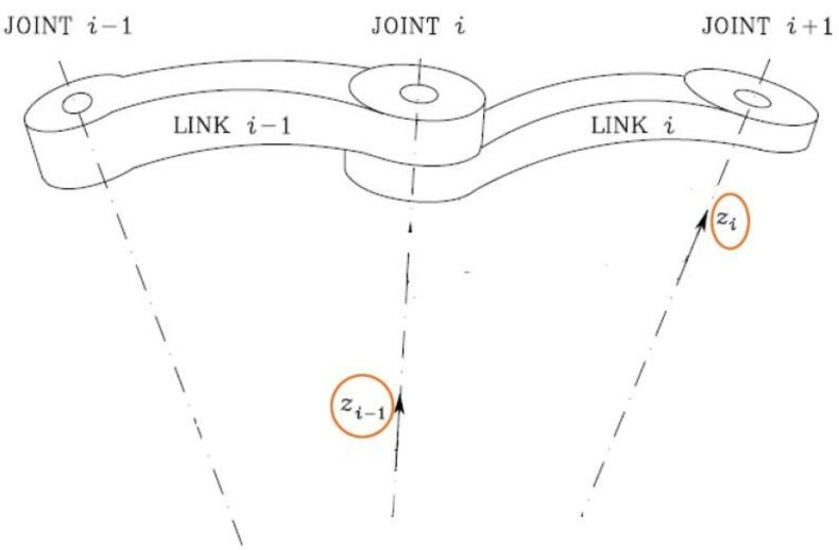
\includegraphics[width=0.8\linewidth]{DH_Images/DH_1.jpg}
        \end{center}
    \end{minipage}

    \item
    \begin{minipage}[t]{0.48\textwidth}
        L'origine \(O_{i}\) del sistema di riferimento \(i\) è posta all'intersezione dell'asse \(z_{i}\) con la normale comune agli assi \(z_{i-1}\) e \(z_{i}\).
    \end{minipage}
    \hfill
    \begin{minipage}[h]{0.48\textwidth}
        \begin{center}
            \centering
            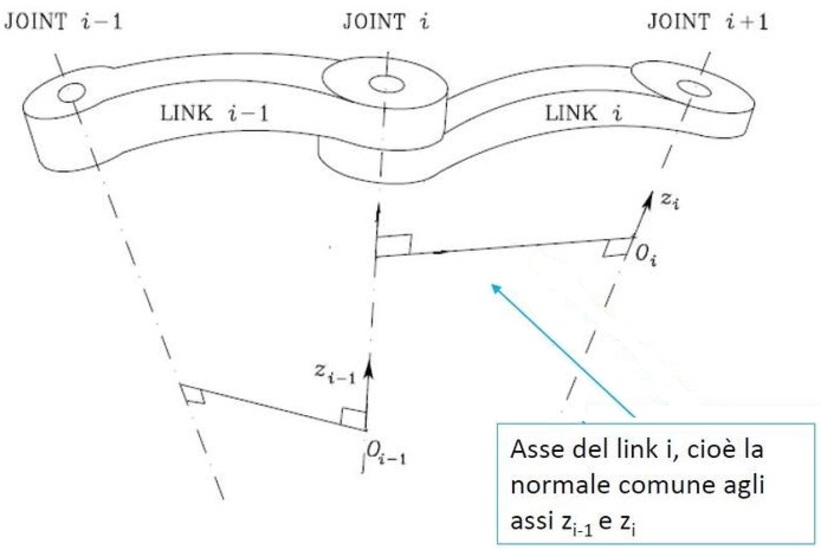
\includegraphics[width=0.8\linewidth]{DH_Images/DH_2.jpg}
        \end{center}
    \end{minipage}

    \item
    \begin{minipage}[t]{0.48\textwidth}
        L'asse \(x_{i}\) è allineato con la normale comune agli assi \(z_{i-1}\) e \(z_{i}\). Il verso positivo è orientato dal giunto \(i\) verso il giunto \(i+1\).
    \end{minipage}
    \hfill
    \begin{minipage}[h]{0.48\textwidth}
        \begin{center}
            \centering
            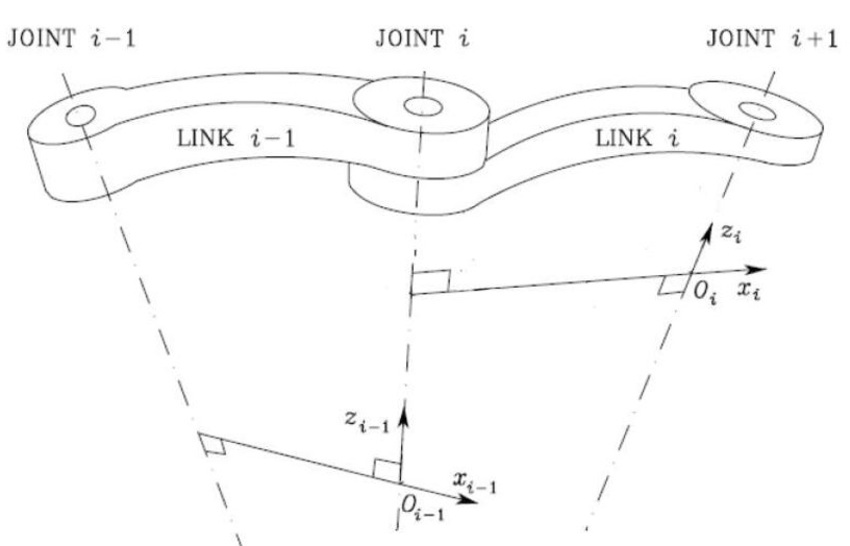
\includegraphics[width=0.75\linewidth]{DH_Images/DH_3.jpg}
        \end{center}
    \end{minipage}

    \item
    \begin{minipage}[t]{0.48\textwidth}
        L'asse \(y_{i}\) è definito in modo da completare una terna cartesiana destrogira, secondo la regola della mano destra (\(y_i = z_i \times x_i\)).
    \end{minipage}
    \hfill
    \begin{minipage}[h]{0.48\textwidth}
        \begin{center}
            \centering
            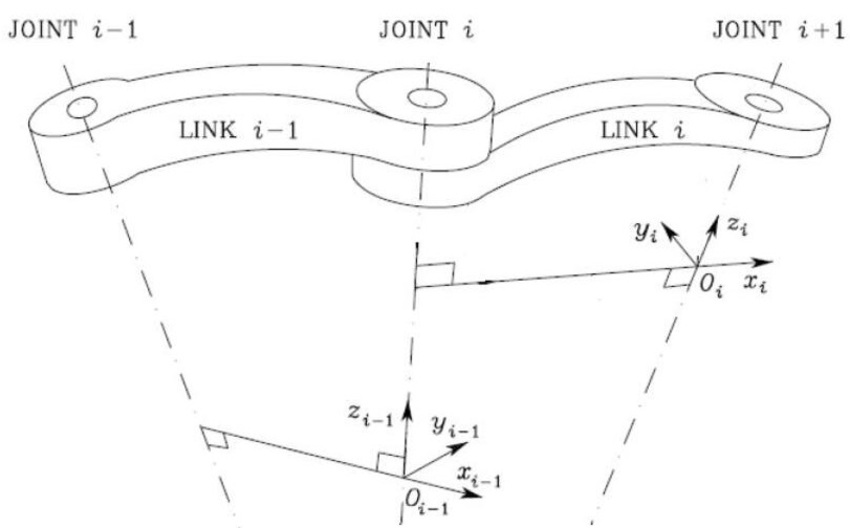
\includegraphics[width=0.75\linewidth]{DH_Images/DH_4.jpg}
        \end{center}
    \end{minipage}
\end{enumerate}
In questo modo, la terna \(i\) definisce il sistema di riferimento \(RF_{i}\) solidale al braccio \(i\).

Questa convenzione presenta alcuni casi di ambiguità, per i quali si seguono delle regole specifiche:
\begin{itemize}
    \item \textbf{Sistema di riferimento di base (\(RF_0\))}: Poiché non esiste un asse \(z_{-1}\), la scelta dell'origine \(O_0\) e della direzione dell'asse \(x_0\) è arbitraria. Tipicamente, \(RF_0\) è fissato alla base del robot.

    \item \textbf{Sistema di riferimento finale (\(RF_n\))}: Non esistendo il giunto \(n+1\), la direzione dell'asse \(z_n\) non è univocamente determinata e può essere scelta liberamente (spesso si allinea con \(z_{n-1}\)). Di conseguenza, la scelta di \(O_n\) e \(x_n\) gode di maggiore libertà.

    \item \textbf{Assi \(z_{i-1}\) e \(z_i\) paralleli}: Esistono infinite normali comuni. La scelta dell'origine \(O_{i}\) lungo l'asse \(z_{i}\) è quindi arbitraria.

    \item \textbf{Assi \(z_{i-1}\) e \(z_i\) incidenti}: La normale comune ha lunghezza nulla. In questo caso, l'asse \(x_{i}\) è definito come ortogonale al piano formato da \(z_{i-1}\) e \(z_i\), con verso dato da \(z_{i-1} \times z_i\).
\end{itemize}
\newpage

Una volta definiti i sistemi di riferimento \(RF_{i}\), la posa della terna \(i\) rispetto alla terna \(i-1\) è descritta da quattro parametri.

\begin{minipage}[h]{0.48\textwidth}
    \subsubsection*{Parametro \(\bm{a_{i}}\)}
    Rappresenta la distanza tra gli assi \(z_{i-1}\) e \(z_{i}\), misurata lungo l'asse \(x_i\). È un parametro fisso che dipende dalla geometria del braccio \(i\).
\end{minipage}
\hfill
\begin{minipage}[h]{0.48\textwidth}
    \begin{center}
        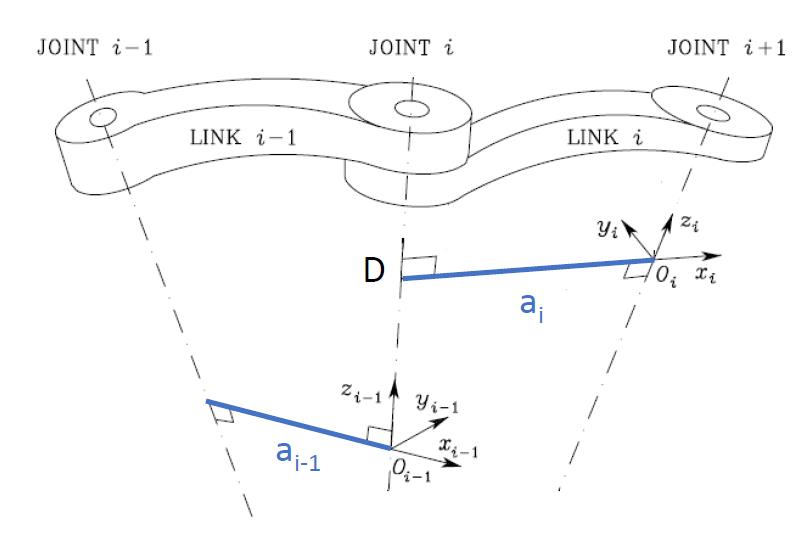
\includegraphics[width=0.75\linewidth]{DH_Images/DH_5.jpg}
    \end{center}
\end{minipage}

\vspace{1cm}

\begin{minipage}[h]{0.48\textwidth}
\subsubsection*{Parametro \(\bm{d_{i}}\)}
    Rappresenta la distanza tra gli assi \(x_{i-1}\) e \(x_{i}\), misurata lungo l'asse \(z_{i-1}\). Se il giunto \(i\) è prismatico, \(d_i\) è la variabile di giunto. Altrimenti, è un parametro fisso.
\end{minipage}
\hfill
\begin{minipage}[h]{0.48\textwidth}
    \begin{center}
        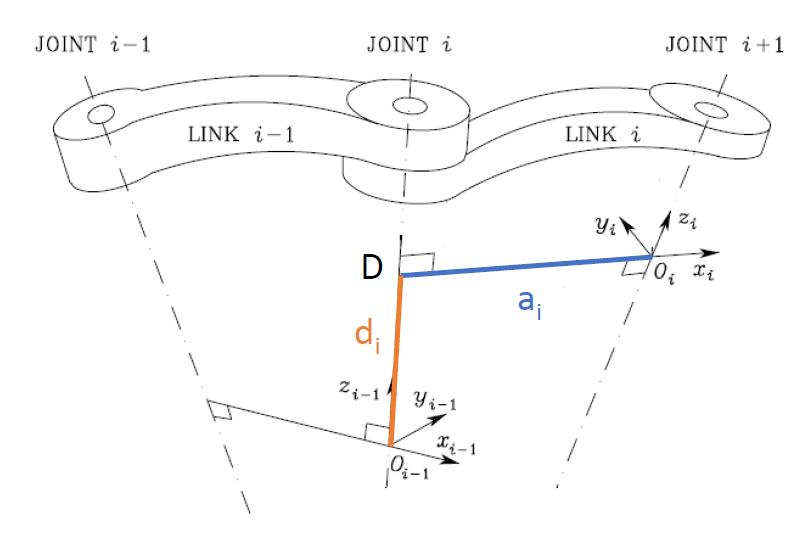
\includegraphics[width=0.75\linewidth]{DH_Images/DH_6.jpg}
    \end{center}
\end{minipage}

\vspace{1cm}

\begin{minipage}[h]{0.48\textwidth}
    \subsubsection*{Parametro \(\bm{\alpha_{i}}\)}
    Rappresenta l'angolo tra gli assi \(z_{i-1}\) e \(z_i\), misurato intorno all'asse \(x_i\). Questo parametro, detto \textit{twist}, è fisso e dipende dalla geometria del braccio \(i\). La convenzione del segno positivo è una rotazione antioraria da \(z_{i-1}\) a \(z_i\) vista lungo \(x_i\).
\end{minipage}
\hfill
\begin{minipage}[h]{0.48\textwidth}
    \begin{center}
        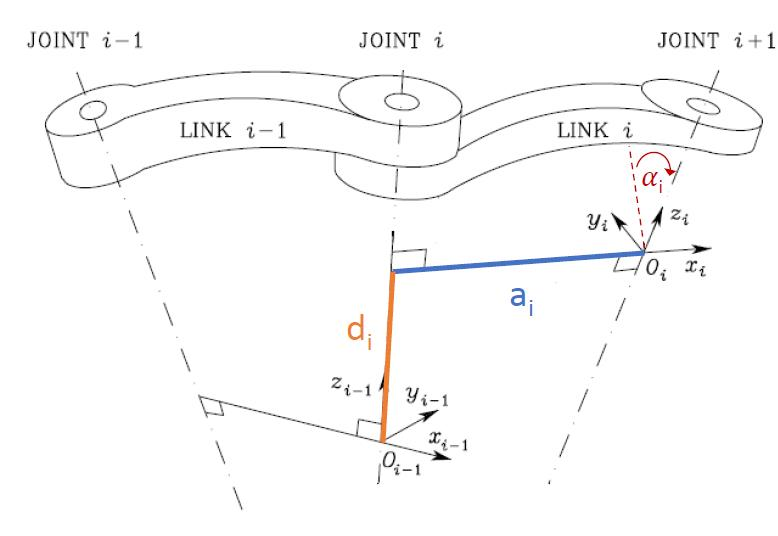
\includegraphics[width=0.75\linewidth]{DH_Images/DH_7.jpg}
    \end{center}
\end{minipage}

\vspace{1cm}

\begin{minipage}[h]{0.45\textwidth}
    \subsubsection*{Parametro \(\bm{\theta_{i}}\)}
    Rappresenta l'angolo tra gli assi \(x_{i-1}\) e \(x_i\), misurato intorno all'asse \(z_{i-1}\). Se il giunto \(i\) è rotoidale, \(\theta_i\) è la variabile di giunto. Altrimenti, è un parametro fisso. La convenzione del segno positivo è una rotazione antioraria da \(x_{i-1}\) a \(x_i\) vista lungo \(z_{i-1}\).
\end{minipage}
\hfill
\begin{minipage}[h]{0.45\textwidth}
    \begin{center}
        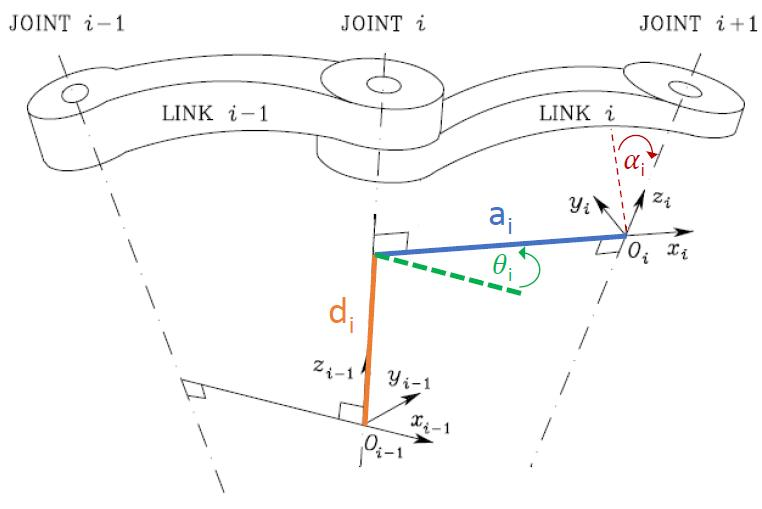
\includegraphics[width=0.75\textwidth]{DH_Images/DH_8.jpg}
    \end{center}
\end{minipage}

\newpage
I parametri DH (\(a_{i}\), \(d_{i}\), \(\alpha_{i}\), \(\theta_{i}\)) permettono di definire la trasformazione omogenea per passare dal sistema di riferimento \(i-1\) al sistema \(i\) attraverso due passaggi elementari.

\begin{itemize}
    \item \textbf{Passaggio 1: Trasformazione lungo e attorno a \(z_{i-1}\)}\\
    Si definisce una terna intermedia \(i'\) applicando una rotazione di angolo \(\theta_i\) e una traslazione di distanza \(d_i\) rispetto all'asse \(z_{i-1}\).
    \begin{center}
        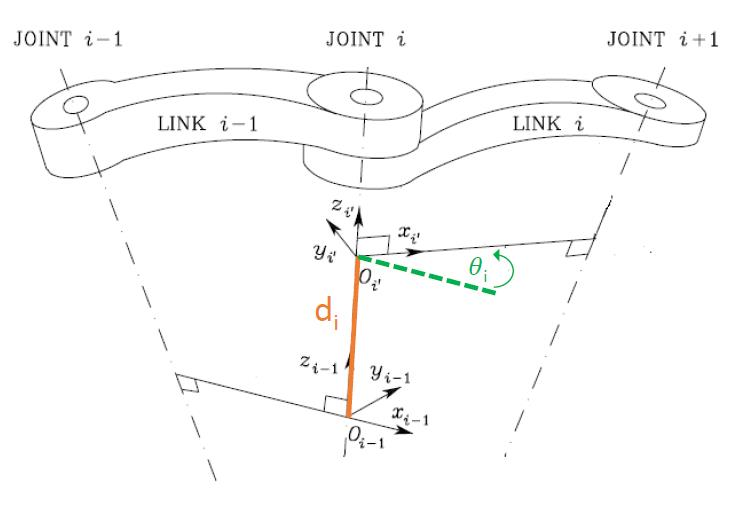
\includegraphics[width=0.5\textwidth]{DH_Images/DH_9.jpg}
    \end{center}
    La matrice di trasformazione omogenea $^{i-1}\bm{A}_{i'}(q_i)$ è data dal prodotto di una rotazione e una traslazione:
    \[
        ^{i-1}\bm{A}_{i'}(q_i) = \text{Rot}(z_{i-1}, \theta_i) \cdot \text{Trasl}(z_{i-1}, d_i) =
        \begin{bmatrix}
            \cos(\theta_i) & -\sin(\theta_i) & 0 & 0 \\
            \sin(\theta_i) & \cos(\theta_i) & 0 & 0 \\
            0 & 0 & 1 & d_i \\
            0 & 0 & 0 & 1
        \end{bmatrix}
    \]
\end{itemize}

\begin{itemize}
    \item \textbf{Passaggio 2: Trasformazione lungo e attorno a \(x_{i}\)}\\
    Dalla terna intermedia \(i'\), si ottiene la terna finale \(i\) applicando una traslazione di distanza \(a_i\) e una rotazione di angolo \(\alpha_i\) rispetto all'asse \(x_i\).
    \begin{center}
        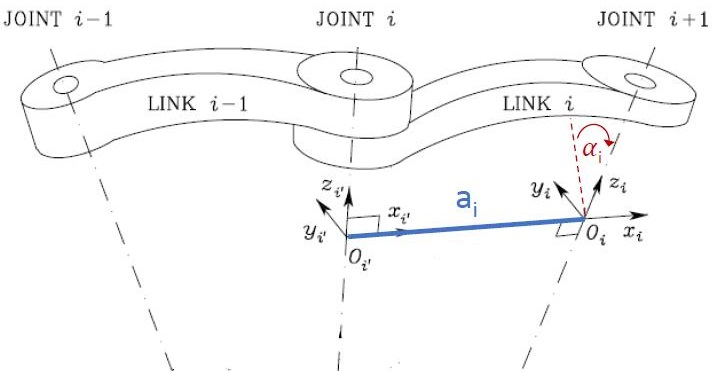
\includegraphics[width=0.5\textwidth]{DH_Images/DH_10.jpg}
    \end{center}
    La matrice corrispondente, \(^{i'}\bm{A}_{i}\), è:
    \[
        ^{i'}\bm{A}_{i} = \text{Trasl}(x_{i}, a_i) \cdot \text{Rot}(x_{i}, \alpha_i) =
        \begin{bmatrix}
            1 & 0 & 0 & a_{i}\\
            0 & \cos(\alpha_i) & -\sin(\alpha_i) & 0 \\
            0 & \sin(\alpha_i) & \cos(\alpha_i) & 0 \\
            0 & 0 & 0 & 1 \\
        \end{bmatrix}
    \]
\end{itemize}

\noindent Svolgendo il prodotto matriciale $^{i - 1}\bm{A}_{i}(q_{i}) = \; ^{i - 1}\bm{A}_{i'}(q_{i}) \cdot {^{i'}\bm{A}_{i}}$, si ottiene la matrice di trasformazione completa di Denavit-Hartenberg:
\[
    ^{i - 1}\bm{A}_{i}(q_{i}) =
    \begin{bmatrix}
        \cos(\theta_i) & -\sin(\theta_i)\cos(\alpha_{i}) & \sin(\theta_i)\sin(\alpha_{i}) & a_{i}\cos(\theta_{i})\\
        \sin(\theta_i) & \cos(\theta_i)\cos(\alpha_{i}) & -\cos(\theta_i)\sin(\alpha_{i}) & a_{i}\sin(\theta_{i})\\
        0 & \sin(\alpha_{i}) & \cos(\alpha_{i}) & d_{i}\\
        0 & 0 & 0 & 1
    \end{bmatrix}
\]
\newpage
Una volta definita la matrice di trasformazione omogenea \(^{i-1}\mathbf{A}_{i}\) per un singolo link, è possibile risolvere il problema della cinematica diretta, ovvero determinare la posa (posizione e orientamento) dell'organo terminale (end-effector) rispetto al sistema di riferimento di base (\(RF_0\)).

È fondamentale notare che la matrice \(^{i-1}\mathbf{A}_{i}\) è funzione di un'unica variabile di giunto \(q_i\), mentre i restanti tre parametri DH sono costanti definite dalla geometria del manipolatore.
\[
    q_{i} =
    \begin{cases}
        \theta_{i} \qquad&\text{se il giunto è rotoidale}\\
        d_{i} \qquad&\text{se il giunto è prismatico}\\
    \end{cases}
\]
Per ottenere la posa finale dell'end-effector (solidale al sistema \(RF_n\)) rispetto alla base (\(RF_0\)), si moltiplicano in catena le singole matrici di trasformazione, dalla base fino all'ultimo giunto:
\[
    ^{0}\bm{T}_{n} = {^{0}\bm{A}_{1}(q_{1})} \cdot {^{1}\bm{A}_{2}(q_{2})} \cdot \dots \cdot {^{n-1}\bm{A}_{n}(q_{n})}
\]
La matrice risultante $^{0}\bm{T}_{n}$ contiene la descrizione completa della posa dell'end-effector. In particolare, il vettore posizione della sua origine, denotato con $^{0}\bm{P}_{EE}$, corrisponde alla quarta colonna della matrice. Matematicamente, questo è equivalente al calcolo:
\[
    \begin{bmatrix}
        ^{0}\bm{P}_{EE} \\
        1
    \end{bmatrix}
    = {^{0}\bm{T}_{n}} \cdot
    \begin{bmatrix}
        0 \\ 0 \\ 0 \\ 1
    \end{bmatrix}
\]



\newpage
% --- Riga 1 ---
\begin{minipage}[t]{0.48\textwidth}
    \subsubsection*{Manipolatore RR}
    \centering
    \begin{tabular}{|c|c|c|c|c|}
        \hline
        \textbf{\# Link} & \(\boldsymbol{\theta}\) & \(\boldsymbol{d}\) & \(\boldsymbol{\alpha}\) & \(\boldsymbol{a}\) \\
        \hline
        1 & \(q_{1}\) & 0 & 0 & \(a_{1}\) \\
        \hline
        2 & \(q_{2}\) & 0 & 0 & \(a_{2}\) \\
        \hline
    \end{tabular}
\end{minipage}
\hfill
\begin{minipage}[t]{0.48\textwidth}
    \subsubsection*{Manipolatore RRR}
    \centering
    \begin{tabular}{|c|c|c|c|c|}
        \hline
        \textbf{\# Link} & \(\boldsymbol{\theta}\) & \(\boldsymbol{d}\) & \(\boldsymbol{\alpha}\) & \(\boldsymbol{a}\) \\
        \hline
        1 & \(q_{1}\) & 0 & 0 & \(a_{1}\) \\
        \hline
        2 & \(q_{2}\) & 0 & 0 & \(a_{2}\) \\
        \hline
        3 & \(q_{3}\) & 0 & 0 & \(a_{3}\) \\
        \hline
    \end{tabular}
\end{minipage}

\vspace{1cm} % Spazio verticale tra le righe di minipage

% --- Riga 2 ---
\begin{minipage}[t]{0.48\textwidth}
    \subsubsection*{Manipolatore RPR}
    \centering
    \begin{tabular}{|c|c|c|c|c|}
        \hline
        \textbf{\# Link} & \(\boldsymbol{\theta}\) & \(\boldsymbol{d}\) & \(\boldsymbol{\alpha}\) & \(\boldsymbol{a}\) \\
        \hline
        1 & \(q_{1}\) & 0 & \(\frac{\pi}{2}\) & 0\\
        \hline
        2 & \(\frac{\pi}{2}\) & \(q_{2}\) & \(-\frac{\pi}{2}\) & 0\\
        \hline
        3 & \(q_{3}\) & 0 & 0 & 0\\
        \hline
    \end{tabular}
\end{minipage}
\hfill
\begin{minipage}[t]{0.48\textwidth}
    \subsubsection*{Manipolatore SCARA}
    \centering
    \begin{tabular}{|c|c|c|c|c|}
        \hline
        \textbf{\# Link} & \(\boldsymbol{\theta}\) & \(\boldsymbol{d}\) & \(\boldsymbol{\alpha}\) & \(\boldsymbol{a}\) \\
        \hline
        1 & \(q_{1}\) & \(d_{1}\) & 0 & \(a_{1}\) \\
        \hline
        2 & \(q_{2}\) & 0 & \(\pi\) & \(a_{2}\) \\
        \hline
        3 & 0 & \(q_{3}\) & 0 & 0 \\
        \hline
        4 & \(q_{4}\) & \(d_{4}\) & 0 & 0 \\
        \hline
    \end{tabular}

\end{minipage}

\vspace{1cm} % Spazio verticale tra le righe di minipage

% --- Riga 3 ---
\begin{minipage}[t]{0.48\textwidth}
    \subsubsection*{Manipolatore Cilindrico}
    \centering
    \begin{tabular}{|c|c|c|c|c|}
        \hline
        \textbf{\# Link} & \(\boldsymbol{\theta}\) & \(\boldsymbol{d}\) & \(\boldsymbol{\alpha}\) & \(\boldsymbol{a}\) \\
        \hline
        1 & \(q_{1}\) & \(d_{1}\) & 0 & 0 \\
        \hline
        2 & \(-\frac{\pi}{2}\) & \(q_{2}\) & \(\frac{\pi}{2}\) & 0\\
        \hline
        3 & 0 & \(q_{3}\) & 0 & 0 \\
        \hline
    \end{tabular}

\end{minipage}
\hfill
\begin{minipage}[t]{0.48\textwidth}
    \subsubsection*{Manipolatore Sferico}
    \centering
    \begin{tabular}{|c|c|c|c|c|}
        \hline
        \textbf{\# Link} & \(\boldsymbol{\theta}\) & \(\boldsymbol{d}\) & \(\boldsymbol{\alpha}\) & \(\boldsymbol{a}\) \\
        \hline
        1 & \(q_{1}\) & \(d_{1}\) & \(\frac{\pi}{2}\) & 0 \\
        \hline
        2 & \(q_{2}\) & 0 & \(-\frac{\pi}{2}\) & 0\\
        \hline
        3 & 0 & \(q_{3}\) & 0 & 0 \\
        \hline
    \end{tabular}
\end{minipage}

\vspace{1cm} % Spazio verticale tra le righe di minipage

% --- Riga 4 (NUOVA) ---
\begin{minipage}[t]{0.48\textwidth}
    \subsubsection*{Manipolatore di Stanford}
    \centering
    \begin{tabular}{|c|c|c|c|c|}
        \hline
        \textbf{\# Link} & \(\boldsymbol{\theta}\) & \(\boldsymbol{d}\) & \(\boldsymbol{\alpha}\) & \(\boldsymbol{a}\) \\
        \hline
        1 & \(q_{1}\) & \(d_{1}\) & \(-\frac{\pi}{2}\) & 0 \\
        \hline
        2 & \(q_{2}\) & \(d_{2}\) & \(\frac{\pi}{2}\) & 0 \\
        \hline
        3 & 0 & \(q_{3}\) & 0 & 0 \\
        \hline
        4 & \(q_{4}\) & 0 & \(-\frac{\pi}{2}\) & 0 \\
        \hline
        5 & \(q_{5}\) & 0 & \(\frac{\pi}{2}\) & 0 \\
        \hline
        6 & \(q_{6}\) & \(d_{6}\) & 0 & 0 \\
        \hline
    \end{tabular}
\end{minipage}
\hfill
\begin{minipage}[t]{0.48\textwidth}
    \subsubsection*{Manipolatore Antropomorfo (6R)}
    \centering
    \begin{tabular}{|c|c|c|c|c|}
        \hline
        \textbf{\# Link} & \(\boldsymbol{\theta}\) & \(\boldsymbol{d}\) & \(\boldsymbol{\alpha}\) & \(\boldsymbol{a}\) \\
        \hline
        1 & \(q_{1}\) & 0 & \(-\frac{\pi}{2}\) & 0 \\
        \hline
        2 & \(q_{2}\) & 0 & 0 & \(a_{2}\) \\
        \hline
        3 & \(q_{3}\) & 0 & \(-\frac{\pi}{2}\) & \(a_{3}\) \\
        \hline
        4 & \(q_{4}\) & \(d_{4}\) & \(\frac{\pi}{2}\) & 0 \\
        \hline
        5 & \(q_{5}\) & 0 & \(-\frac{\pi}{2}\) & 0 \\
        \hline
        6 & \(q_{6}\) & \(d_{6}\) & 0 & 0 \\
        \hline
    \end{tabular}
\end{minipage}

\newpage


\subsubsection*{Esempio: Posizione dell'End-Effector del Manipolatore RPR}

Applichiamo il metodo generale al manipolatore RPR. Le matrici di trasformazione omogenea per ciascun giunto sono:
\begin{align*}
    ^{0}\bm{A}_{1}(q_{1}) &=
    \begin{bmatrix}
        \cos(q_{1}) & 0 & -\sin(q_{1}) & 0\\
        \sin(q_{1}) & 0 & \cos(q_{1}) & 0\\
        0 & -1 & 0 & A\\
        0 & 0 & 0 & 1
    \end{bmatrix} \\
    ^{1}\bm{A}_{2}(q_{2}) &=
    \begin{bmatrix}
        0 & 0 & 1 & 0\\
        -1 & 0 & 0 & 0\\
        0 & -1 & 0 & q_{2}\\
        0 & 0 & 0 & 1
    \end{bmatrix} \\
    ^{2}\bm{A}_{3}(q_{3}) &=
    \begin{bmatrix}
        \cos(q_{3}) & -\sin(q_{3}) & 0 & B\cos(q_{3})\\
        \sin(q_{3}) & \cos(q_{3}) & 0 & B\sin(q_{3})\\
        0 & 0 & 1 & 0\\
        0 & 0 & 0 & 1
    \end{bmatrix}
\end{align*}

La matrice di trasformazione totale dalla base all'end-effector è $^{0}\bm{T}_{3} = {^{0}\bm{A}_{1}} \cdot {^{1}\bm{A}_{2}} \cdot {^{2}\bm{A}_{3}}$. Eseguendo il prodotto:
\[
    ^{0}\bm{T}_{3} =
    \begin{bmatrix}
        \cos(q_1) & 0 & -\sin(q_1) & 0 \\
        \sin(q_1) & 0 & \cos(q_1) & 0 \\
        0 & -1 & 0 & A \\
        0 & 0 & 0 & 1
    \end{bmatrix}
    \begin{bmatrix}
        - \sin(q_3) & - \cos(q_3) & 0 & - B \sin(q_3) \\
        - \cos(q_3) & \sin(q_3) & 0 & B \cos(q_3) \\
        0 & 0 & -1 & -q_2 \\
        0 & 0 & 0 & 1
    \end{bmatrix}
\]
\[
    ^{0}\bm{T}_{3} =
    \begin{bmatrix}
        -\cos(q_1)\sin(q_3) & -\cos(q_1)\cos(q_3) & \sin(q_1) & B\sin(q_1)\sin(q_3) - q_2\sin(q_1) \\
        -\sin(q_1)\sin(q_3) & -\sin(q_1)\cos(q_3) & -\cos(q_1) & -B\cos(q_1)\sin(q_3) + q_2\cos(q_1) \\
        \cos(q_3) & -\sin(q_3) & 0 & A+B\cos(q_3) \\
        0 & 0 & 0 & 1
    \end{bmatrix}
\]
Il vettore posizione dell'origine dell'end-effector (\(EE\)) rispetto alla base è la quarta colonna di $^{0}\bm{T}_{3}$:
\[
    ^{0}\bm{P}_{EE} =
    \begin{bmatrix}
        B\sin(q_{1})\sin(q_{3}) - q_{2}\sin(q_{1}) \\
        q_{2}\cos(q_{1}) - B\cos(q_{1})\sin(q_{3}) \\
        A + B\cos(q_{3})
    \end{bmatrix}
\]
\newpage
\subsubsection{Singolarità Cinematiche}

Le singolarità cinematiche sono configurazioni specifiche di un manipolatore in cui la sua capacità di muoversi o di esercitare forze in determinate direzioni nello spazio operativo è ridotta. In queste pose, il robot perde uno o più gradi di libertà, e la mappatura tra lo spazio dei giunti e lo spazio operativo cessa di essere biunivoca.

Dal punto di vista del problema cinematico inverso, una singolarità si manifesta come l'impossibilità di determinare in modo univoco le variabili di giunto necessarie per raggiungere una data posa dell'end-effector. Questo fenomeno è spesso noto come \textbf{gimbal lock}, dove due assi di rotazione del robot si allineano, rendendo i loro effetti indistinguibili.

\subsubsection*{Analisi Singolarità Di Rappresentazione}
Per analizzare questa condizione, si consideri un orientamento dell'end-effector descritto da una sequenza di tre rotazioni elementari, come gli angoli di Eulero XYZ:
\[
    \mathbf{R}(\phi, \theta, \psi) = \mathbf{R}_{X}(\phi) \mathbf{R}_{Y}(\theta) \mathbf{R}_{Z}(\psi)
\]
L'obiettivo è dimostrare che questa rappresentazione diventa singolare per un valore critico di \(\theta\). Per farlo, si sfrutta un'identità che permette di esprimere una rotazione attorno a un asse tramite rotazioni attorno ad altri due. Nello specifico, la rotazione attorno all'asse \(x\) può essere riscritta come:
\[
    \mathbf{R}_{X}(\phi) = \mathbf{R}_{Y}\left(\frac{\pi}{2}\right) \mathbf{R}_{Z}(\phi) \mathbf{R}_{Y}\left(-\frac{\pi}{2}\right)
\]
Sostituendo questa espressione nella formula dell'orientamento, si raggruppano i termini per analizzarne l'interazione:
\[
    \mathbf{R}(\phi, \theta, \psi) = \left[ \mathbf{R}_{Y}\left(\frac{\pi}{2}\right) \mathbf{R}_{Z}(\theta) \mathbf{R}_{Y}\left(-\frac{\pi}{2}\right) \right] \mathbf{R}_{Y}(\theta) \mathbf{R}_{Z}(\psi)
\]
Si esamina ora il caso particolare in cui il giunto intermedio assume il valore critico \( \theta = \frac{\pi}{2} \). La parte centrale dell'espressione diventa il prodotto di due rotazioni opposte attorno allo stesso asse \(Y\), che si annullano a vicenda (risultando nella matrice identità \(\mathbf{I}\)):
\[
    \mathbf{R}_{Y}\left(-\frac{\pi}{2}\right) \mathbf{R}_{Y}\left(\frac{\pi}{2}\right) = \mathbf{I}
\]
La matrice di rotazione totale si semplifica drasticamente:
\begin{align*}
    \mathbf{R}\left(\phi, \frac{\pi}{2}, \psi\right) &= \mathbf{R}_{Y}\left(\frac{\pi}{2}\right) \mathbf{R}_{Z}(\phi) \left[ \mathbf{R}_{Y}\left(-\frac{\pi}{2}\right) \mathbf{R}_{Y}\left(\frac{\pi}{2}\right) \right] \mathbf{R}_{Z}(\psi) \\
    &= \mathbf{R}_{Y}\left(\frac{\pi}{2}\right) \mathbf{R}_{Z}(\phi) \mathbf{I} \mathbf{R}_{Z}(\psi) \\
    &= \mathbf{R}_{Y}\left(\frac{\pi}{2}\right) \left[ \mathbf{R}_{Z}(\phi) \mathbf{R}_{Z}(\psi) \right] \\
    &= \mathbf{R}_{Y}\left(\frac{\pi}{2}\right) \mathbf{R}_{Z}(\phi + \psi)
\end{align*}

Il risultato finale \(\mathbf{R} = \mathbf{R}_{Y}(\frac{\pi}{2}) \mathbf{R}_{Z}(\phi + \psi)\), mostra che l'orientamento dell'end-effector non dipende più individualmente da \(\phi\) e \(\psi\), ma solo dalla loro \textbf{somma}. Questo significa che infinite combinazioni dei due angoli producono lo stesso identico orientamento. Ad esempio, se \(\phi + \psi = 45^\circ\), le coppie \((45^\circ, 0^\circ)\), \((30^\circ, 15^\circ)\) e \((0^\circ, 45^\circ)\) sono tutte soluzioni valide per lo stesso problema cinematico inverso.

Questa singolarità ha implicazioni significative e problematiche nel controllo del manipolatore:
\begin{itemize}
    \item \textbf{Ambiguità Cinematica Inversa:} In una configurazione singolare esistono infinite soluzioni per i giunti, rendendo impossibile sceglierne una in modo univoco.

    \item \textbf{Instabilità Controllo:} In prossimità di una singolarità, la matrice Jacobiana del manipolatore diventa singolare. Ciò implica che per generare piccole variazioni di velocità dell'end-effector in certe direzioni, sarebbero necessarie velocità di giunto teoricamente infinite. Questo può portare a movimenti incontrollati e potenziali danni al robot.

    \item \textbf{Complessità Nella Pianificazione Della Traiettoria:} I percorsi dell'end-effector devono essere pianificati attentamente per evitare di attraversare o avvicinarsi a configurazioni singolari.
\end{itemize}

\newpage
\section{Cinematica Inversa}
La \textbf{cinematica inversa} di un robot definisce il problema di calcolare i valori delle variabili di giunto, indicati con \( \mathbf{q} \), necessari affinché l'End Effector raggiunga una determinata posizione e orientamento nello spazio. A differenza della cinematica diretta, che determina la posa dell'end-effector a partire dai valori dei giunti, il problema inverso è notevolmente più complesso per diverse ragioni. Le principali criticità sono:

\begin{enumerate}
    \item \textbf{Non Linearità Delle Equazioni}: Le equazioni matematiche che governano la cinematica inversa sono non lineari. Di conseguenza, trovare una soluzione analitica in forma chiusa è spesso impossibile, rendendo necessario il ricorso a metodi numerici o approssimati per la loro risoluzione.

    \item \textbf{Soluzioni Multiple}: Per una singola posizione e orientamento dell'end-effector, possono esistere molteplici configurazioni dei giunti che soddisfano la richiesta. Questa molteplicità di soluzioni richiede la scelta di quella più ottimale, basata su criteri come il consumo di energia o la minimizzazione degli spostamenti.

    \item \textbf{Infinite Soluzioni Per Manipolatori Ridondanti}: Un manipolatore è definito \textit{ridondante} quando possiede un numero di gradi di libertà superiore a quello strettamente necessario per compiere un'operazione. In tali casi, il problema della cinematica inversa ammette un numero infinito di soluzioni, poiché esistono innumerevoli configurazioni dei giunti in grado di realizzare la stessa posa finale.

    \item \textbf{Assenza Di Soluzioni Ammissibili}: È possibile che non esista alcuna configurazione di giunto in grado di raggiungere la posa desiderata. Questo si verifica quando il punto target si trova al di fuori dello spazio di lavoro del robot, a causa di limitazioni fisiche e geometriche intrinseche alla sua struttura.
\end{enumerate}

La risoluzione della cinematica inversa rappresenta una sfida fondamentale in robotica e viene affrontata con diversi approcci, tra cui metodi analitici, numerici, scelti in base alla complessità del manipolatore. In sintesi, data la posa desiderata dell'organo terminale, espressa dalla matrice di trasformazione omogenea:
\[
    \bm{T} =
    \begin{bmatrix}
        \bm{R} & \bm{P}\\
        \bm{0}_{1\times 3} & 1
    \end{bmatrix}
\]
L'obiettivo è determinare un vettore di variabili di giunto \( \mathbf{q} \) tale che la matrice di trasformazione calcolata dalla cinematica diretta, \(^{0}\bm{A}_{n}(\mathbf{q})\), coincida con \(\bm{T}\).

Le principali sfide di questo problema includono:
\begin{itemize}
    \item La necessità di risolvere equazioni non lineari, per le quali non sempre esiste una soluzione analitica.
    \item La possibilità che le equazioni ammettano soluzioni multiple o infinite.
    \item L'eventualità che, a causa della struttura del manipolatore, non esistano soluzioni ammissibili.
\end{itemize}
\newpage
\subsection{Spazio dei Giunti e Spazio di Lavoro}
Per analizzare l'esistenza di soluzioni al problema della cinematica inversa, si definiscono due insiemi fondamentali che caratterizzano lo spazio di lavoro di un manipolatore:

\begin{itemize}
    \item \textbf{Workspace Primario \( W_{S1} \) (Spazio Raggiungibile)}: È l'insieme di tutti i punti \( p \) che l'end-effector del manipolatore è in grado di raggiungere con \textit{almeno un} orientamento \( \phi \) (o una rotazione \( R \)). Se un punto si trova al di fuori di questo spazio, il problema della cinematica inversa non ammette soluzioni. Al contrario, se un punto \( p \) appartiene a \( W_{S1} \), esiste almeno una configurazione dei giunti che permette di raggiungerlo.
        \begin{flalign*}
            & WS_{1} = \biggl\{ p \in \mathbb{R}^{3} \; : \; \exists \, q \; : \; f(q) = p\biggr\}\\
            & p \; \notin \; WS_{1} \quad\longrightarrow\quad \nexists \; q\\
            & p \; \in \; WS_{1} \quad\longrightarrow\quad \exists \; q
        \end{flalign*}

    \item \textbf{Workspace Secondario \( W_{S2} \) (Spazio di Destrezza)}: È l'insieme dei punti \( p \) che l'end-effector può raggiungere con \textit{qualsiasi} orientamento fisicamente realizzabile. Un punto appartenente a \( W_{S2} \) garantisce la massima destrezza del manipolatore, poiché la sua posizione può essere raggiunta con un'orientazione arbitraria.
    \[
        WS_{2} = \biggl\{ p \in \mathbb{R}^{3} \; : \forall \, \bm{R} \in SO(3) \; \exists \, q \; : \; ^{0}A_{n}(q) =
        \begin{bmatrix}
            \bm{R} & \bm{p}\\
            \bm{0}_{1\times 3} & 1
        \end{bmatrix}
        \biggr\}
    \]
\end{itemize}

Per definizione, lo Spazio di Destrezza è un sottoinsieme dello Spazio Raggiungibile (\( W_{S2} \subseteq W_{S1} \)). Lo spazio di lavoro complessivo del manipolatore è determinato dalla sua geometria e dai vincoli meccanici imposti sui suoi giunti.

La risolvibilità del problema della cinematica inversa è garantita solo se la posa desiderata (posizione e orientamento) appartiene allo spazio di lavoro del manipolatore.

\subsubsection*{Esempio}
Consideriamo un manipolatore planare \textbf{RR} (due giunti rotoidali). I suoi spazi di lavoro primario e secondario dipendono dalla relazione tra le lunghezze dei suoi due bracci, \( l_1 \) e \( l_2 \).

\paragraph{Caso 1: \(l_1 \neq l_2\)}
In questa configurazione, gli spazi di lavoro sono definiti come segue:
\begin{itemize}
    \item \textbf{Spazio Operativo Primario (\(WS_1\))}: È una corona circolare centrata nell'origine, con raggio interno \(|l_1 - l_2|\) e raggio esterno \(l_1 + l_2\). Questi limiti rappresentano, rispettivamente, la minima e la massima distanza che l'end-effector può raggiungere dall'origine.
    $$
        WS_{1} = \big\{ p \in \mathbb{R}^2 : |l_{1} - l_{2}| \leq \|p\| \leq l_{1} + l_{2} \big\}.
    $$

    \item \textbf{Spazio Operativo Secondario (\(WS_2\))}: È l'insieme vuoto, poiché non esiste alcun punto che possa essere raggiunto con un orientamento arbitrario.
    $$
    WS_2 = \emptyset.
    $$
\end{itemize}

\paragraph{Caso 2: \(l_1 = l_2 = l\)}
Quando i due bracci hanno la stessa lunghezza, gli spazi di lavoro cambiano come segue:
\begin{itemize}
    \item \textbf{Spazio Operativo Primario (\(WS_1\))}: Diventa un disco pieno centrato nell'origine con raggio \(2l\). La distanza massima è la somma delle lunghezze (\(l+l=2l\)), mentre la minima è zero, ottenibile quando i bracci sono ripiegati l'uno sull'altro.
    $$
    WS_1 = \big\{ p \in \mathbb{R}^2 : \|p\| \leq 2l \big\}.
    $$

    \item \textbf{Spazio Operativo Secondario (\(WS_2\))}: Si riduce al solo punto di origine. L'origine è l'unico punto che può essere raggiunto con qualsiasi orientamento dell'end-effector.
    $$
    WS_2 = \{0\}.
    $$
\end{itemize}

\newpage
\subsection{Cinematica Manipolatore RR Planare}

\begin{minipage}[c]{0.45\textwidth}
    Lo spazio operativo rappresenta tutte le posizioni e orientazioni che l'utensile (end-effector) può raggiungere. In questo caso, lo spazio operativo ha dimensione $m = 3$ ed è descritto dal vettore:
    \[
        \mathbf{r} =
        \begin{bmatrix}
        P_x \\
        P_y \\
        \phi
        \end{bmatrix}
    \]
    Dove  $P_x$ e $P_y$ sono le coordinate cartesiane dell'end-effector nel piano e $\phi$ è l'orientazione dell'end-effector rispetto all'asse orizzontale positivo.

    Le variabili di giunto descrivono le configurazioni del manipolatore. In questo caso, la dimensione delle variabili di giunto è $n = 2$ e sono descritte dal vettore:
    \[
        \mathbf{q} =
        \begin{bmatrix}
        q_1 \\
        q_2
        \end{bmatrix}
    \]
    Dove $q_1$ è l'angolo del primo braccio rispetto all'asse orizzontale e $q_2$ è l'angolo relativo tra il primo e il secondo braccio
\end{minipage}
\hfill
\begin{minipage}[c]{0.45\textwidth}
    \centering
    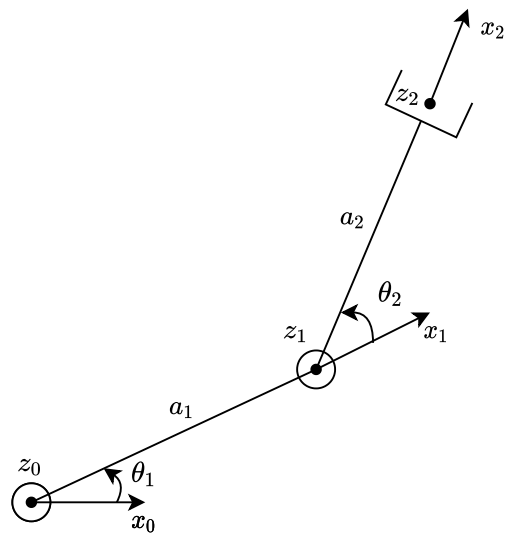
\includegraphics[width=0.9\linewidth]{RR_Planare.png}
\end{minipage}


\subsubsection{Cinematica Diretta}
Un robot planare con due giunti rotazionali (RR) ha il primo braccio di lunghezza \( l_1 \), il cui estremo si trova a una distanza \( l_1 \) dall'origine e forma un angolo \( q_1 \) rispetto all'asse orizzontale. Le sue coordinate cartesiane sono quindi:
\[
    x_1 = l_1 \cos q_1 \qquad y_1 = l_1 \sin q_1.
\]
L'end-effector è situato all'estremità del secondo braccio, che ha lunghezza \( l_2 \) e forma un angolo totale di \( q_1 + q_2 \) rispetto all'asse orizzontale. Le sue coordinate cartesiane sono date da:
\[
    P_x = x_1 + l_2 \cos (q_1 + q_2) \qquad P_y = y_1 + l_2 \sin (q_1 + q_2).
\]

Sostituendo le espressioni di \( x_1 \) e \( y_1 \), si ottiene la formulazione completa della cinematica diretta:
\[
    P_x = l_1 \cos q_1 + l_2 \cos (q_1 + q_2) \qquad
    P_y = l_1 \sin q_1 + l_2 \sin (q_1 + q_2).
\]

L'orientazione dell'end-effector è data dalla somma degli angoli dei due giunti:
\[
    \phi = q_1 + q_2.
\]

Pertanto, la posizione e l'orientazione dell'end-effector possono essere espresse in forma vettoriale come:
\[
    \mathbf{r} = f(q) =
    \begin{bmatrix}
        P_x \\
        P_y \\
        \phi
    \end{bmatrix}
    =
    \begin{bmatrix}
        l_1 \cos(q_1) + l_2 \cos (q_1 + q_2) \\
        l_1 \sin(q_1) + l_2 \sin (q_1 + q_2) \\
        q_1 + q_2
    \end{bmatrix}.
\]

\newpage
\subsubsection{Cinematica Inversa}
Dai risultati della cinematica diretta si nota che
\[
    x^{2} + y^{2} = \biggl[ l_1 \cos(q_1) + l_2 \cos (q_1 + q_2) \biggr]^{2} + \biggl[ l_1 \sin(q_1) + l_2 \sin (q_1 + q_2) \biggr]^{2} =
\]
\[
    = \biggl[ l_{1}^{2} \cos^{2}(q_1) + 2\biggl( l_{1} \cos (q_1) \biggr)\biggl(l_{2} \cos (q_1 + q_2)\biggr) + l_{2}^{2} \cos^{2} (q_1 + q_2) \biggr] +
\]
\[
    + \biggl[ l_{1}^{2} \sin^{2}(q_1) + 2\biggl( l_1 \sin(q_1) \biggr) \biggl( l_2 \sin (q_1 + q_2) \biggr) + l_{2}^{2} \sin^{2} (q_1 + q_2) \biggr] =
\]
\[
    = l_{1}^{2}\biggl[ \cos^{2}(q_1) + \sin^{2}(q_1) \biggr] + 2l_{1}l_{2}\biggl[ \cos (q_1)\cos (q_1 + q_2) + \sin(q_1)\sin(q_1 + q_2) \biggr] + l_{2}^{2}\biggl[ \cos^{2}(q_1 + q_2) + \sin^{2}(q_1 + q_2) \biggr] =
\]
Ricordando che \(\cos^{2}(\theta) + \sin^{2}(\theta) = 1\), si ottiene
\[
    = l_{1}^{2} + 2l_{1}l_{2}\biggl[ \cos (q_1)\cos (q_1 + q_2) + \sin(q_1)\sin(q_1 + q_2) \biggr] + l_{2}^{2}
\]
Quindi, si ottiene che
\[
    x^{2} + y^{2} = l_{1}^{2} + l_{2}^{2} + 2l_{1}l_{2}\biggl[ \cos (q_1)\cos (q_1 + q_2) + \sin(q_1)\sin(q_1 + q_2) \biggr]
\]
\[
    x^{2} + y^{2} - \biggr( l_{1}^{2} + l_{2}^{2} \biggl) =  2l_{1}l_{2}\biggl[ \cos (q_1)\cos (q_1 + q_2) + \sin(q_1)\sin(q_1 + q_2) \biggr]
\]
Ricordando la formula
\[
    \cos(\theta - \phi) = \cos(\theta)\cos(\phi) + \sin(\theta)\sin(\phi)
\]
E ponendo \(\theta = q_{1}\) e \(\phi = q_{1} + q_{2}\), quindi si può scrivere come
\[
    x^{2} + y^{2} - \biggr( l_{1}^{2} + l_{2}^{2} \biggl) =  2l_{1}l_{2} \cos\bigg[ q_{1} - \biggl(q_{1} + q_{2}\biggr) \biggr]
\]\[
    x^{2} + y^{2} - \biggr( l_{1}^{2} + l_{2}^{2} \biggl) =  2l_{1}l_{2} \cos\big( - q_{2}\ \bigr)
\]
Sapendo che il coseno è pari si ha che \(\cos(-q_2) = \cos(q_2)\) e di conseguenza
\[
    x^{2} + y^{2} - \biggr( l_{1}^{2} + l_{2}^{2} \biggl) =  2l_{1}l_{2} \cos\big(q_{2}\ \bigr)
\]
Da cui si può calcolare
\begin{flalign*}
    & cos(q_{2}) = \displaystyle{ \frac{x^{2} + y^{2} - \biggr( l_{1}^{2} + l_{2}^{2} \biggl)}{2l_{1}l_{2}} }\\
    & sin(q_{2}) = \displaystyle{ \pm \sqrt{1 - \cos^{2}(q_{2}) \;\; } }
\end{flalign*}
Da cui, usando l'arcotangente a quattro quadranti si ottiene:
\[
    \boxed{q_{2} = \text{atan2}\biggl(\sin(q_{2}), \; \cos(q_{2}) \biggr)}
\]

Nella cinematica inversa del manipolatore RR planare, esistono generalmente due possibili soluzioni per $ q_{2} $, corrispondenti a due diverse configurazioni del braccio:
\begin{itemize}
    \item \textbf{Gomito Alto ($ \bm{+} $)}: Il gomito è sopra la linea che collega la base all'effettore finale

    \item \textbf{Gomito Basso ($ \bm{-} $)}: Il gomito è sotto la linea che collega la base all'effettore finale.
\end{itemize}
Queste due configurazioni derivano dal fatto che il manipolatore può raggiungere la stessa posizione finale con due diverse disposizioni delle articolazioni.

\subsubsection*{Caso particolare: $ \sqrt{1 - \cos^2(q_2)} = 0 \;\longrightarrow\;  \sin(q_2) = 0 $}
Ricordando l'identità trigonometrica fondamentale $\sin^2(q_2) + \cos^2(q_2) = 1$ si può dire che:
\[
    \sin^2(q_2) = 1 - \cos^2(q_2) \quad\longrightarrow\quad \sin(q_2) = \pm\sqrt{1 - \cos^2(q_2)}
\]
La condizione $ \sqrt{1 - \cos^2(q_2)} = 0 $ implica quindi che $ \sin(q_2) = 0 $. Questa situazione si verifica per due valori specifici dell'angolo $q_2$ nell'intervallo $[0, 2\pi)$:

\begin{itemize}
    \item \(q_{2} = 0 \): Il secondo braccio è allineato con il primo, e il manipolatore è nella sua massima estensione (configurazione "braccio teso").
    \item \(q_{2} = \pi \): Il secondo braccio è ripiegato sul primo, e il manipolatore è nella sua minima estensione (configurazione "braccio piegato").
\end{itemize}
In entrambi questi scenari, il manipolatore si trova in una \textbf{configurazione singolare} o \textbf{degenere}. In queste pose, l'end effector si trova sull'asse del primo braccio, e non è più possibile distinguere geometricamente tra le due soluzioni della cinematica inversa (definite "gomito alto" e "gomito basso"). Questo rappresenta un caso limite che richiede particolare attenzione nell'implementazione degli algoritmi di cinematica inversa.

Per trovare una soluzione per $q_1$, si parte dalle equazioni della cinematica diretta. Ricordando le formule di addizione per seno e coseno:
\begin{flalign*}
    & \cos(\theta + \phi) = \cos(\theta)\cos(\phi) - \sin(\theta)\sin(\phi) & \\
    & \sin(\theta + \phi) = \sin(\theta)\cos(\phi) + \cos(\theta)\sin(\phi) &
\end{flalign*}

Le equazioni della cinematica diretta del manipolatore RR sono:
\[
    \begin{cases}
        x = l_1 \cos(q_1) + l_2 \cos(q_1 + q_2) \\
        y = l_1 \sin(q_1) + l_2 \sin(q_1 + q_2)
    \end{cases}
\]
Applichiamo le formule di addizione ai termini $\cos(q_1 + q_2)$ e $\sin(q_1 + q_2)$ e sostituendo queste espressioni nelle equazioni di partenza, si ottiene:
\[
    \begin{cases}
        x = l_1 \cos(q_1) + l_2\biggl[\cos(q_{1})\cos(q_{2}) - \sin(q_{1})\sin(q_{2}) \biggr] \\
        y = l_1 \sin(q_1) + l_2\biggl[ \sin(q_{1})\cos(q_{2}) + \cos(q_{1})\sin(q_{2}) \biggr]
    \end{cases}
\]
Svolgendo i calcoli e raccogliendo i termini in base a $\cos(q_1)$ e $\sin(q_1)$ per isolare le variabili legate a $q_1$.
\[
    \begin{cases}
        x = l_1 \cos(q_1) + l_2\cos(q_{1})\cos(q_{2}) - l_2\sin(q_{1})\sin(q_{2}) \\
        y = l_1 \sin(q_1) + l_2\sin(q_{1})\cos(q_{2}) + l_2\cos(q_{1})\sin(q_{2})
    \end{cases}
\]
Raccogliendo i fattori comuni:
\[
    \begin{cases}
        x = \biggl[l_1 + l_2\cos(q_{2})\biggr]\cos(q_1) - \biggl[l_2\sin(q_{2}) \biggr]\sin(q_{1}) \\
        y = \biggl[l_1 + l_2\cos(q_{2})\biggr]\sin(q_1) + \biggl[l_2\sin(q_{2}) \biggr]\cos(q_{1})
    \end{cases}
\]
Riordinando i termini questo sistema di equazioni lineari nelle incognite $\cos(q_1)$ e $\sin(q_1)$ può essere espresso elegantemente in forma matriciale:
\[
    \begin{bmatrix}
        x\\
        y
    \end{bmatrix}
    =
    \;\;
    \underbrace{\begin{bmatrix}
        l_1 + l_2\cos(q_{2}) & - l_2\sin(q_{2})\\
        l_2\sin(q_{2}) & l_1 + l_2\cos(q_{2})
    \end{bmatrix}}_{\pi(q_{2})}
    \quad
    \begin{bmatrix}
        \cos(q_1)\\
        \sin(q_1)
    \end{bmatrix}
\]
Questa forma è molto utile perché evidenzia come le coordinate cartesiane $(x, y)$ siano il risultato di una trasformazione lineare (che dipende solo da $q_2$) applicata al vettore delle componenti trigonometriche di $q_1$.

Per poter risolvere il sistema e trovare $\cos(q_1)$ e $\sin(q_1)$, si deve invertire la matrice $\pi(q_2)$. Una matrice è invertibile se e solo se il suo determinante è diverso da zero. Quindi:
\[
    \det\bigl[ \pi(q_{2}) \bigr] =  \bigl( l_1 + l_2 \cos(q_2) \bigr) \cdot \bigl( l_1 + l_2 \cos(q_2) \bigr) - \bigl( -l_2 \sin(q_2) \bigr) \cdot \bigl( l_2 \sin(q_2) \bigr)
\]
\[
    \det\bigl[ \pi(q_{2}) \bigr] =  \bigl( l_1 + l_2 \cos(q_2) \bigr)^2 + \bigl( l_2 \sin(q_2) \bigr)^2
\]
Sviluppando il quadrato del binomio:
\[
    \det\bigl[ \pi(q_{2}) \bigr] =  \biggl( l_{1}^{2} + 2 l_{1} l_{2} \cos(q_{2}) + l_{2}^{2} \cos^{2}(q_{2}) \biggr) + \biggl( l_{2}^{2} \sin^{2}(q_{2}) \biggr)
\]
Raccogliendo $l_2^2$ e utilizzando l'identità $\cos^2(q_2) + \sin^2(q_2) = 1$:
\[
    \det\bigl[ \pi(q_{2}) \bigr] = l_{1}^{2} + 2 l_{1} l_{2} \cos(q_{2}) + l_{2}^{2} \bigl(\cos^{2}(q_{2}) + \sin^{2}(q_{2})\bigr)
\]
\[
    \det\bigl[ \pi(q_{2}) \bigr] = l_{1}^{2} + 2 l_{1} l_{2} \cos(q_{2}) + l_{2}^{2}
\]
Quindi si avrà che il determinante è nullo se le condizioni $l_1 = l_2$ e $\cos(q_2) = -1$ sono verificate simultaneamente perché in questo caso si avrebbe
\[
    \det\bigl[ \pi(q_{2}) \bigr] = l^{2} + 2 l^{2} (-1) + l^{2} = 2l^{2} - 2l^{2} = 0
\]
In questo caso, il braccio è completamente ripiegato su se stesso e l'end effector si trova nell'origine $(0,0)$.
Se $ \det\bigl[ \pi(q_{2}) \bigr] = 0 $, la matrice $\pi(q_2)$ non è invertibile e ci troviamo in una \textbf{singolarità cinematica}.

Se, invece, il determinante è strettamente positivo, si può invertire la matrice e risolvere per il vettore $[\cos(q_1), \sin(q_1)]^T$:
\[
    \begin{bmatrix}
        \cos(q_1)\\
        \sin(q_1)
    \end{bmatrix}
    =
    \begin{bmatrix}
        l_1 + l_2\cos(q_{2}) & - l_2\sin(q_{2})\\
        l_2\sin(q_{2}) & l_1 + l_2\cos(q_{2})
    \end{bmatrix}^{-1}
    \begin{bmatrix}
        x\\
        y
    \end{bmatrix}
\]

Una volta calcolati i valori numerici di $\sin(q_1)$ e $\cos(q_1)$ risolvendo il sistema, si può determinare l'angolo $q_1$ in modo univoco utilizzando la funzione arcotangente a due argomenti. Questa funzione è preferibile alla semplice arcotangente perché risolve l'ambiguità del quadrante analizzando i segni sia del seno che del coseno.
\[
    \boxed{q_{1} = \text{atan2} \biggl(\sin(q_{1}), \; \cos(q_{1}) \biggr)}
\]


\subsubsection*{Approccio Alternativo Basato Sulla Geometria Vettoriale}
Un modo alternativo per affrontare il problema è considerare la cinematica diretta in forma vettoriale. La posizione dell'end effector $P(x,y)$ è la somma dei vettori posizione dei due bracci. Utilizzando le matrici di rotazione $R(\theta)$:
\[
    \begin{bmatrix}
        x \\
        y
    \end{bmatrix}
    =
    \underbrace{R(q_1)
    \begin{bmatrix}
        l_1 \\
        0
    \end{bmatrix}}_{\text{Vettore del primo braccio}}
    +
    \underbrace{R(q_1 + q_2)
    \begin{bmatrix}
        l_2 \\
        0
    \end{bmatrix}}_{\text{Vettore del secondo braccio}}
\]
Questa equazione può essere riordinata per isolare il contributo del primo braccio:
\[
    \begin{bmatrix}
        x \\
        y
    \end{bmatrix}
    -R(q_1 + q_2)
    \begin{bmatrix}
        l_2 \\
        0
    \end{bmatrix}
    =
    R(q_1)
    \begin{bmatrix}
        l_1 \\
        0
    \end{bmatrix}
\]
Questa formulazione è la base per un'altra tecnica di soluzione della cinematica inversa, dove tipicamente si eleva al quadrato la norma di entrambi i lati per eliminare $q_1$ e risolvere prima per $q_2$. Da lì, si può poi ricavare $q_1$ e infine l'angolo $\theta$. Questo approccio geometrico è spesso più intuitivo e porta alla stessa soluzione finale.
\newpage
\subsubsection*{Caso Del Manipolatore RRR Planare}
Estendendo le osservazioni fatte per il manipolatore RR planare al caso del manipolatore RRR planare, la cinematica diretta può essere espressa come segue:

\[
    \begin{bmatrix}
    x \\
    y
    \end{bmatrix}
    =
    R(q_1 + q_2 + q_3)
    \begin{bmatrix}
    l_3 \\
    0
    \end{bmatrix}
    +
    R(q_1 + q_2)
    \begin{bmatrix}
    l_2 \\
    0
    \end{bmatrix}
    +
    R(q_1)
    \begin{bmatrix}
    l_1 \\
    0
    \end{bmatrix}.
\]


Per risolvere il problema della cinematica inversa, si possono sfruttare i risultati già ottenuti per il manipolatore RR planare. La precedente si può scrivere come:

\[
\underbrace{
    \begin{bmatrix}
    x \\
    y
    \end{bmatrix}
    -
    R(q_1 + q_2 + q_3)
    \begin{bmatrix}
    l_3 \\
    0
    \end{bmatrix}
    }_{\begin{bmatrix}
    \hat{x} \\
    \hat{y}
    \end{bmatrix}}
    =
    R(q_1 + q_2)
    \begin{bmatrix}
    l_2 \\
    0
    \end{bmatrix}
    +
    R(q_1)
    \begin{bmatrix}
    l_1 \\
    0
    \end{bmatrix}.
\]

Si nota che il problema si riduce a quello di un manipolatore RR planare, dove si deve determinare $ q_1 $ e $ q_2 $ in base alla nuova posizione $ (\hat{x}, \hat{y}) $.

Il vincolo geometrico per la raggiungibilità della posizione $ (\hat{x}, \hat{y}) $ è dato da:

\[
|l_1 - l_2| \leq \sqrt{\hat{x}^2 + \hat{y}^2} \leq l_1 + l_2.
\]

Questo vincolo assicura che la distanza $ \sqrt{\hat{x}^2 + \hat{y}^2} $ sia compatibile con le lunghezze dei segmenti $ l_1 $ e $ l_2 $. Se è soddisfatto, si possono calcolare $ q_1 $ e $ q_2 $ utilizzando i metodi già descritti per il manipolatore RR planare. Una volta determinati $ q_1 $ e $ q_2 $, l'angolo $ q_3 $ può essere ricavato come:

\[
q_3 = (q_1 + q_2 + q_3) - (q_1 + q_2).
\]

\newpage
\subsection*{Metodi Per La Risoluzione Di Equazioni Trigonometriche}

Nella cinematica inversa dei manipolatori, un passaggio cruciale è spesso la risoluzione di un'equazione trigonometrica nella forma:
\[
    a \sin(\theta) + b \cos(\theta) = c
\]
Questa equazione permette di determinare un angolo di giunto \( \theta \) a partire dalle componenti cartesiane. Esistono due approcci principali e molto efficaci per risolverla.

\subsubsection*{Metodo 1: Sostituzione Con Formule Parametriche}

Questo metodo, puramente algebrico, trasforma l'equazione trigonometrica in un'equazione polinomiale. Il trucco consiste nell'utilizzare una sostituzione ponendo:
\[
    u = \tan \frac{\theta}{2}
\]
Grazie a questa sostituzione, le funzioni \( \sin(\theta) \) e \( \cos(\theta) \) possono essere espresse come funzioni razionali di \( u \):
\[
    \sin(\theta) = \frac{2u}{1 + u^2} \qquad \qquad \qquad \cos(\theta) = \frac{1 - u^2}{1 + u^2}
\]
Sostituendo queste espressioni nell'equazione originale si ottiene:
\[
    a \left( \frac{2u}{1 + u^2} \right) + b \left( \frac{1 - u^2}{1 + u^2} \right) = c
\]
Per eliminare i denominatori, moltiplichiamo entrambi i membri per \( (1 + u^2) \), assumendo che non sia nullo (il che è sempre vero per \( u \) reali):
\[
    a(2u) + b(1 - u^2) = c(1 + u^2)
\]
Espandendo e riordinando i termini per raggrupparli secondo le potenze di \( u \) e portando tutti i termini sullo stesso lato per ottenere un'equazione omogenea, si ottiene
\[
    (b + c)u^2 - 2au + (c - b) = 0
\]
Questa è un'equazione quadratica standard nella variabile \( u \). Si può risolve usando la formula per le equazioni di secondo grado, che fornirà due possibili soluzioni per \( u \):
\[
    u_{1,2} = \frac{-B \pm \sqrt{B^2 - 4AC}}{2A} = \frac{2a \pm \sqrt{4a^{2} - 4(b+c)(c-b)}}{2(b+c)}
\]
Se il discriminante \( (4a^2 - 4(b+c)(c-b)) \) è non negativo, si ottengono una o due soluzioni reali per \( u \). Infine, per trovare i valori corrispondenti di \( \theta \), si inverte la sostituzione iniziale:
\[
    \frac{\theta_{1,2}}{2} = \arctan(u_{1,2}) \qquad \longrightarrow \qquad \theta_{1,2} = 2 \arctan(u_{1,2})
\]
Questo metodo è robusto e sistematico, ma può nascondere l'intuizione geometrica del problema.


\newpage
\subsubsection*{Metodo 2: Metodo Angolo Ausiliario (Forma Ampiezza-Fase)}

Questo secondo approccio è più elegante e geometricamente intuitivo. L'idea è di riconoscere che la combinazione lineare di un seno e un coseno con lo stesso argomento è equivalente a una singola funzione trigonometrica con ampiezza e fase modificate.

Si può riscrivere il lato sinistro dell'equazione \( a \sin(\theta) + b \cos(\theta) \) nella forma \( A \cos(\theta - \phi) \). Espandendo questa espressione con la formula di sottrazione del coseno, si ottiene:
\[
    A \cos(\theta - \phi) = A (\cos\theta \cos\phi + \sin\theta \sin\phi) = (A\sin\phi)\sin\theta + (A\cos\phi)\cos\theta
\]
Confrontando questa forma con l'originale \( a \sin(\theta) + b \cos(\theta) \), si possono uguagliare i coefficienti:
\begin{align*}
    a &= A \sin(\phi) \\
    b &= A \cos(\phi)
\end{align*}
Da questo sistema si possono ricavare \( A \) e \( \phi \). Elevando al quadrato e sommando le due equazioni si ottiene l'ampiezza \( A \):
\[
    a^2 + b^2 = A^2(\sin^2\phi + \cos^2\phi) = A^2 \qquad \longrightarrow \qquad A = \sqrt{a^2 + b^2}
\]
Per trovare l'angolo di fase \( \phi \), si possono dividere le due equazioni, ottenendo \( \tan(\phi) = a/b \). Per determinare univocamente il quadrante di \( \phi \), si usa la funzione arcotangente a quattro quadranti:
\[
    \phi = \operatorname{atan2}(a, b)
\]
L'equazione originale si trasforma quindi in:
\[
    A \cos(\theta - \phi) = c
\]
Ora si può risolverla facilmente per \( \theta \). Prima di tutto, si nota che una soluzione reale può esistere solo se \( |c| \le A \), ovvero \( c^2 \le a^2 + b^2 \). Se questa condizione è soddisfatta:
\[
    \cos(\theta - \phi) = \frac{c}{A}
\]
Applicando l'arcocoseno, che fornisce due soluzioni simmetriche:
\[
    \theta - \phi = \pm \arccos\left(\frac{c}{A}\right)
\]
Infine, isolando \( \theta \) otteniamo le due possibili soluzioni:
\[
    \theta_{1,2} = \phi \pm \arccos\left(\frac{c}{\sqrt{a^2 + b^2}}\right)
\]
Questo metodo non solo fornisce la soluzione, ma rende anche chiara la condizione geometrica di esistenza della soluzione.

\newpage
\subsection{Disaccoppiamento Polso - Struttura Portante}
Il manipolatore di Stanford è un robot composto da due componenti:
un \textit{Manipolatore Sferico} e un \\
\textit{Polso Sferico}. Questa architettura combinata consente al robot di operare in uno spazio tridimensionale con elevata flessibilità e precisione.

\subsubsection*{Manipolatore Sferico: Cinematica Diretta}
Il manipolatore sferico è caratterizzato da una configurazione cinematica RRP (\textit{Rotoidale-Rotoidale-Prismatico}). La denominazione \texttt{Sferico} deriva dalla forma dello spazio di lavoro del manipolatore, cioè la regione tridimensionale all'interno della quale il manipolatore può muoversi e interagire con gli oggetti.

\begin{minipage}[c]{0.45\textwidth}
    \centering
    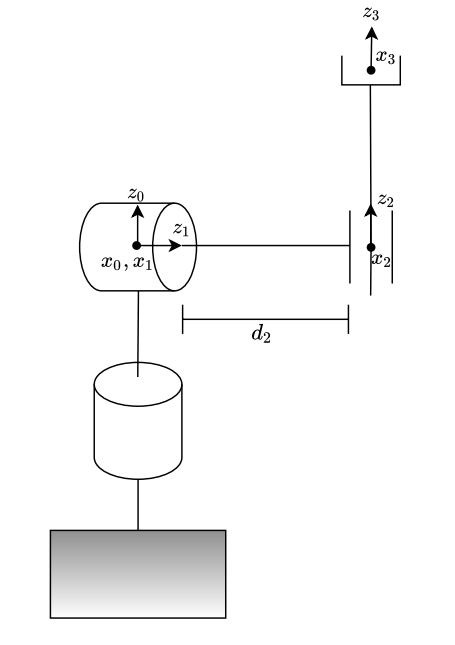
\includegraphics[width=0.75\linewidth]{Fig2_33 Pag 58.png}
\end{minipage}
\hfill
\begin{minipage}[c]{0.45\textwidth}
    \centering
    \begin{tabular}{|c|c|c|c|c|}
        \hline
        \textbf{\# Link} & \(\boldsymbol{\theta}\) & \(\boldsymbol{d}\) & \(\boldsymbol{\alpha}\) & \(\boldsymbol{a}\) \\
        \hline
        1 & \(q_{1}\) & 0 & \(-\frac{\pi}{2}\) & 0 \\
        \hline
        2 & \(q_{2}\) & \(d_{2}\) & \(\frac{\pi}{2}\) & 0 \\
        \hline
        3 & 0 & \(q_{3}\) & 0 & 0 \\
        \hline
    \end{tabular}
\end{minipage}

Le matrici di trasformazione omogenea sono:
\[
    ^{0}\bm{A}_{1}(q_{1}) =
    \begin{bmatrix}
        \cos(q_{1}) & 0 & -\sin(q_{1}) & 0\\
        \sin(q_{1}) & 0 & \cos(q_{1}) & 0\\
        0 & -1 & 0 & 0\\
        0 & 0 & 0 & 1
    \end{bmatrix}
    \qquad\qquad
    ^{1}\bm{A}_{2}(q_{2}) =
    \begin{bmatrix}
        \cos(q_{2}) & 0 & \sin(q_{2}) & 0\\
        \sin(q_{2}) & 0 & -\cos(q_{2}) & 0\\
        0 & 1 & 0 & d_{2}\\
        0 & 0 & 0 & 1
    \end{bmatrix}
\]
\[
    ^{2}\bm{A}_{3}(q_{3}) =
    \begin{bmatrix}
        1 & 0 & 0 & 0\\
        0 & 1 & 0 & 0\\
        0 & 0 & 1 & q_{3}\\
        0 & 0 & 0 & 1
    \end{bmatrix}
\]
E quindi
\[
    ^{0}\bm{T}_{3}(\textbf{q}) \; = \; ^{0}\bm{A}_{1}(q_{1}) \; \cdot \; ^{1}\bm{A}_{2}(q_{2}) \; \cdot \; ^{2}\bm{A}_{3}(q_{3}) =
\]

\[
    =
    \begin{bmatrix}
        c(q_{1})c(q_{2}) & -s(q_{1}) & c(q_{1})s(q_{2}) & c(q_{1})s(q_{2})q_{3} - s(q_{1})d_{2} \\
        s(q_{1})c(q_{2}) & c(q_{1}) & s(q_{1})s(q_{2}) & s(q_{1})s(q_{2})q_{3} + c(q_{1})d_{2}\\
        -s(q_{2}) & 0 & c(q_{2}) & c(q_{2})q_{3}\\
        0 & 0 & 0 & 1
    \end{bmatrix}
\]
% COMBACIA CON CALCOLO MATLAB MANIPOLATORE SFERICO (TIPO II)
\newpage
\subsubsection*{Polso Sferico: Cinematica Diretta}
Il polso sferico è caratterizzato da una configurazione cinematica RRR (\textit{Rotoidale-Rotoidale-Rotoidale}). La denominazione \texttt{Sferico} deriva dal fatto che i tre assi si intersecano in un punto comune, detto \textit{Centro Del Polso}

\begin{minipage}[c]{0.45\textwidth}
    \centering
    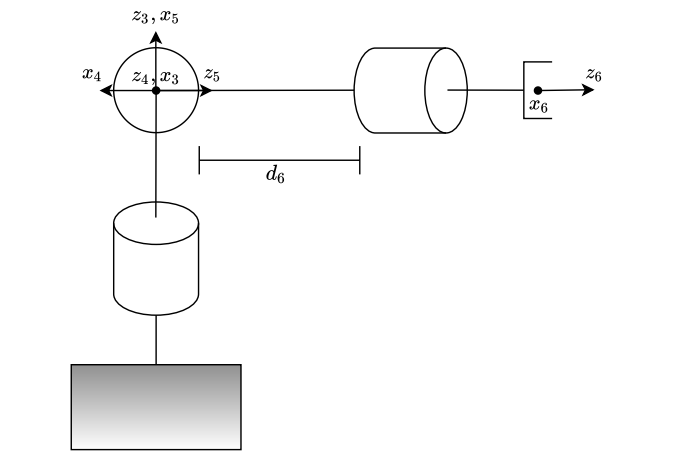
\includegraphics[width=0.9\linewidth]{Fig2_34 Pag 59.png}
\end{minipage}
\hfill
\begin{minipage}[c]{0.45\textwidth}
    % \centering
    \begin{tabular}{|c|c|c|c|c|}
        \hline
        \textbf{\# Link} & \(\boldsymbol{\theta}\) & \(\boldsymbol{d}\) & \(\boldsymbol{\alpha}\) & \(\boldsymbol{a}\) \\
        \hline
        4 & \(q_{4}\) & 0 & \(-\frac{\pi}{2}\) & 0 \\
        \hline
        5 & \(q_{5}\) & 0 & \(\frac{\pi}{2}\) & 0 \\
        \hline
        6 & \(q_{6}\) & \(d_{6}\) & 0 & 0 \\
        \hline
    \end{tabular}
\end{minipage}

Le matrici di trasformazione omogenea sono:
\[
    ^{3}\bm{A}_{4}(q_{4}) =
    \begin{bmatrix}
        \cos(q_{4}) & 0 & -\sin(q_{4}) & 0\\
        \sin(q_{4}) & 0 & \cos(q_{4}) & 0\\
        0 & -1 & 0 & 0\\
        0 & 0 & 0 & 1
    \end{bmatrix}
    \qquad\qquad
    ^{4}\bm{A}_{5}(q_{5}) =
    \begin{bmatrix}
        \cos(q_{5}) & 0 & \sin(q_{5}) & 0\\
        \sin(q_{5}) & 0 & -\cos(q_{5}) & 0\\
        0 & 1 & 0 & 0\\
        0 & 0 & 0 & 1
    \end{bmatrix}
\]
\[
    ^{5}\bm{A}_{6}(q_{6}) =
    \begin{bmatrix}
        \cos(q_{6}) & -\sin(q_{6}) & 0  & 0\\
        \sin(q_{6}) & \cos(q_{6}) & 0 & 0\\
        0 & 0 & 1 & d_{6}\\
        0 & 0 & 0 & 1
    \end{bmatrix}
\]
E quindi
\[
    ^{3}\bm{T}_{6}(\textbf{q}) \; = \; ^{3}\bm{A}_{4}(q_{4}) \; \cdot \; ^{4}\bm{A}_{5}(q_{5}) \; \cdot \; ^{5}\bm{A}_{6}(q_{6}) =
\]

\[
    =
        \begin{bmatrix}
            c(q_{4})c(q_{5})c(q_{6}) - s(q_{4})s(q_{6}) & -c(q_{6})s(q_{4}) - c(q_{4})c(q_{5})s(q_{6}) & c(q_{4})s(q_{5}) & c(q_{4})s(q_{5})d_{6} \\
            c(q_{4})s(q_{6}) + c(q_{5})c(q_{6})s(q_{4}) & c(q_{4})c(q_{6}) - c(q_{5})s(q_{4})s(q_{6}) & s(q_{4})s(q_{5}) & s(q_{4})s(q_{5})d_{6} \\
            -c(q_{6})s(q_{5}) & s(q_{5})s(q_{6}) & c(q_{5}) & c(q_{5})d_{6} \\
            0 & 0 & 0 & 1
        \end{bmatrix}
\]
    % ^{3}\bm{T}_{6} É SICURO GIUSTA COPIATA DA MATLAB
\newpage
\subsubsection*{Manipolatore Di Stanford: Cinematica Diretta}
Poiché, il riferimento \(RF_{3}\) del manipolatore sferico coincide con il riferimento \(RF_{3}\) del polso sferico e di conseguenza la cinematica diretta può essere espressa per composizione delle matrici di trasformazioni

\begin{minipage}[c]{0.4\textwidth}
    \centering
    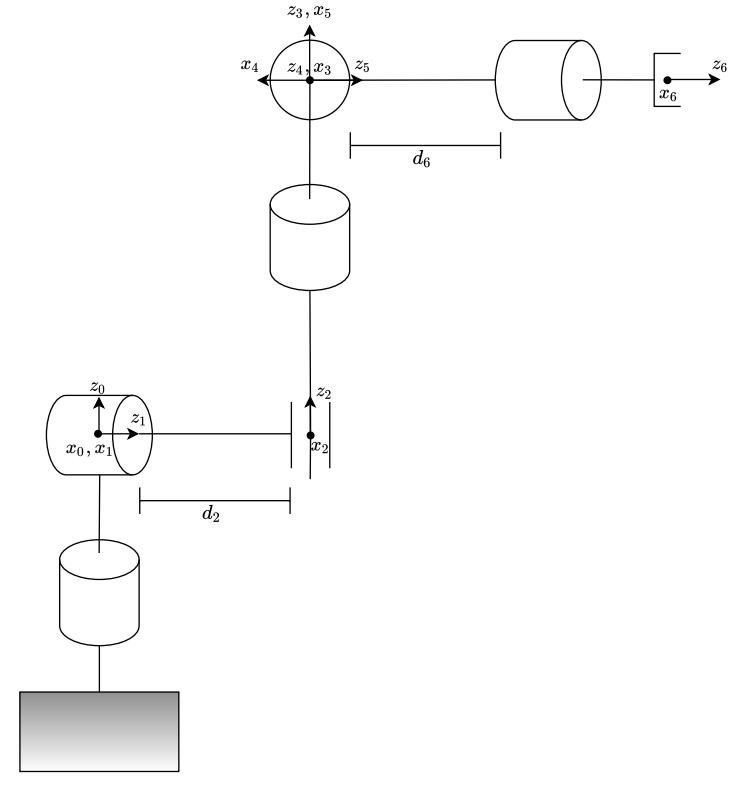
\includegraphics[width=0.99\linewidth]{ManipolatoreStanford.png}
\end{minipage}
\hfill
\begin{minipage}[c]{0.55\textwidth}
    La cinematica diretta del manipolatore completo si ottiene componendo le matrici di trasformazione del braccio e del polso:
    \[
        ^{0}\bm{T}_{6}(\mathbf{q}) \; = \; ^{0}\bm{T}_{3}(\mathbf{q}) \; \cdot \; ^{3}\bm{T}_{6}(\mathbf{q})
    \]
    Il risultato è una matrice di trasformazione omogenea \(4 \times 4\) della forma:
    \[
        ^{0}\bm{T}_{6} =
        \begin{bmatrix}
            \mathbf{A} & \mathbf{B} & \mathbf{C} & \mathbf{D}\\
            0 & 0 & 0 & 1
        \end{bmatrix}
    \]
\end{minipage}

Dove le colonne \(\mathbf{A}\), \(\mathbf{B}\), \(\mathbf{C}\) rappresentano la matrice di rotazione \(^{0}\mathbf{R}_{6}\) e la colonna \(\mathbf{D}\) rappresenta il vettore di posizione \(^{0}\mathbf{p}_{6}\). I loro valori, calcolati simbolicamente, sono i seguenti.

% ---- COLONNA A ----
\[
    \mathbf{A} =
    \begin{bmatrix}
        c(q_{1})c(q_{2})c(q_{4})c(q_{5}) - c(q_{5})s(q_{1})s(q_{4}) - c(q_{1})s(q_{2})s(q_{5})\\
        \\
        c(q_{1})c(q_{5})s(q_{4}) - s(q_{1})s(q_{2})s(q_{5}) + c(q_{2})c(q_{4})c(q_{5})s(q_{1})\\
        \\
        -c(q_{2})s(q_{5}) - c(q_{4})c(q_{5})s(q_{2})
    \end{bmatrix}
\]

% ---- COLONNA B ----
\[
    \mathbf{B} =
    \begin{bmatrix}
        -c(q_{4})s(q_{1}) - c(q_{1})c(q_{2})s(q_{4})\\
        \\
        c(q_{1})c(q_{4}) - c(q_{2})s(q_{1})s(q_{4})\\
        \\
        s(q_{2})s(q_{4})
    \end{bmatrix}
\]

% ---- COLONNA C ----
\[
    \mathbf{C} =
    \begin{bmatrix}
        c(q_{1})c(q_{5})s(q_{2}) - s(q_{1})s(q_{4})s(q_{5}) + c(q_{1})c(q_{2})c(q_{4})s(q_{5})\\
        \\
        c(q_{5})s(q_{1})s(q_{2}) + c(q_{1})s(q_{4})s(q_{5}) + c(q_{2})c(q_{4})s(q_{1})s(q_{5})\\
        \\
        c(q_{2})c(q_{5}) - c(q_{4})s(q_{2})s(q_{5})
    \end{bmatrix}
\]

% ---- COLONNA D ----
\[
    \mathbf{D} =
    \begin{bmatrix}
        d_{2}s(q_{1}) + q_{3}c(q_{1})s(q_{2}) + d_{6}c(q_{1})c(q_{5})s(q_{2}) - d_{6}s(q_{1})s(q_{4})s(q_{5}) + d_{6}c(q_{1})c(q_{2})c(q_{4})s(q_{5})\\
        \\
        q_{3}s(q_{1})s(q_{2}) - d_{2}c(q_{1}) + d_{6}c(q_{5})s(q_{1})s(q_{2}) + d_{6}c(q_{1})s(q_{4})s(q_{5}) + d_{6}c(q_{2})c(q_{4})s(q_{1})s(q_{5})\\
        \\
        q_{3}c(q_{2}) + d_{6}c(q_{2})c(q_{5}) - d_{6}c(q_{4})s(q_{2})s(q_{5})
    \end{bmatrix}
\]
\newpage
\subsubsection{Proprietà di Disaccoppiamento Cinematico}
La struttura del manipolatore di Stanford è progettata per semplificare la risoluzione del problema cinematico inverso grazie a una proprietà nota come \textbf{disaccoppiamento cinematico}. L'obiettivo è determinare le variabili di giunto \(\mathbf{q}\) per raggiungere una posa desiderata, data come matrice di trasformazione omogenea \(^{0}\mathbf{T}_{6}\), che contiene la rotazione \({}^0\mathbf{R}_6\) e la posizione \({}^{0}\mathbf{d}_{6}\) desiderate. Questi due termini sono i \textbf{dati di input noti} del nostro problema, espressi come matrice omogenea:
\[
    ^{0}\mathbf{T}_{6} =
    \begin{bmatrix}
         {}^0\mathbf{R}_6 & {}^{0}\mathbf{d}_{6} \\
         \mathbf{0}_{1 \times 3} & 1
    \end{bmatrix}
\]

La strategia risolutiva consiste nel dividere il problema in due parti:
\begin{enumerate}
    \item \textbf{Cinematica Inversa Di Posizione:} Trovare $(q_1, q_2, q_3)$ per posizionare il \textit{centro del polso}.
    \item \textbf{Cinematica Inversa Di Orientamento:} Trovare $(q_4, q_5, q_6)$ per ottenere l'orientamento finale.
\end{enumerate}
\subsubsection*{Risoluzione Per La Posizione}
Il punto di partenza è l'equazione di posizione che deriva dalla composizione delle trasformazioni \({}^{0}\mathbf{T}_{6} = {}^{0}\mathbf{T}_{3} \cdot {}^{3}\mathbf{T}_{6}\):
\[
    {}^{0}\mathbf{d}_{6} = {}^0\mathbf{R}_3 \, {}^{3}\mathbf{d}_{6} + {}^{0}\mathbf{d}_{3}
\]
Analizziamo i termini di questa equazione nel contesto del problema inverso:
\begin{itemize}
    \item \({}^{0}\mathbf{d}_{6}\): È il \textbf{Vettore Posizione Desiderato} Dell'End-Effector. È un \textbf{dato noto}.
    \item \({}^{0}\mathbf{d}_{3}\) e \({}^0\mathbf{R}_3\): Sono la posizione e l'orientamento del centro del polso. Dipendono solo dai primi tre giunti e sono le \textbf{una delle incognite}.
    \item \({}^{3}\mathbf{d}_{6}\): È la posizione dell'end-effector vista dal centro del polso. Dipende solo dai giunti del polso ed è un'\textbf{altra incognita}.
\end{itemize}
La struttura del polso sferico ci permette di semplificare \({}^{3}\mathbf{d}_{6}\). Questo vettore rappresenta unicamente la traslazione di lunghezza fissa \(d_6\) (un parametro noto del robot) orientata dalla rotazione del polso \({}^3\mathbf{R}_6\):
\[
    {}^{3}\mathbf{d}_{6} = {}^3\mathbf{R}_6
    \begin{bmatrix} 0 \\ 0 \\ d_6 \end{bmatrix}
\]
Sostituendo questa espressione nell'equazione principale e usando la proprietà di composizione delle rotazioni \({}^0\mathbf{R}_6 = {}^0\mathbf{R}_3 \cdot {}^3\mathbf{R}_6\), si ottiene:
\[
    {}^{0}\mathbf{d}_{6} = \underbrace{({}^0\mathbf{R}_3 \cdot {}^3\mathbf{R}_6)}_{{}^0\mathbf{R}_6} \begin{bmatrix} 0 \\ 0 \\ d_6 \end{bmatrix} + {}^{0}\mathbf{d}_{3}
\]
Riordinando l'equazione per isolare le incognite del braccio da un lato e i termini noti dall'altro, si ottiene la formula per la posizione del centro del polso:
\[
    \underbrace{{}^{0}\mathbf{d}_{3}}_{\text{Incognite: } q_1, q_2, q_3} = \underbrace{{}^{0}\mathbf{d}_{6} - {}^0\mathbf{R}_6 \begin{bmatrix} 0 \\ 0 \\ d_6 \end{bmatrix}}_{\text{Termini Noti Dalla Posa Desiderata}}
\]
Il lato destro è ora un vettore numerico calcolabile. Uguagliando questo risultato con l'espressione della cinematica diretta di \({}^{0}\mathbf{d}_{3}\), si possono risolvere $q_1, q_2, q_3$.
\newpage
\subsubsection*{Risoluzione Per L'Orientamento}
Una volta determinati $q_1, q_2, q_3$, la matrice ${}^0\mathbf{R}_3$ è nota. Dalla relazione di composizione delle rotazioni, possiamo calcolare la matrice di rotazione del polso:
\[
    {}^0\mathbf{R}_6 = {}^0\mathbf{R}_3 \cdot {}^3\mathbf{R}_6
\]
Moltiplicando a sinistra per l'inversa di ${}^0\mathbf{R}_3$, che è la sua trasposta $({}^0\mathbf{R}_3)^{T}$, si isola ${}^3\mathbf{R}_6$:
\[
    ({}^0\mathbf{R}_3)^{T} \, {}^0\mathbf{R}_6 = ({}^0\mathbf{R}_3)^{T} \, {}^0\mathbf{R}_3 \, {}^3\mathbf{R}_6
    \qquad\longrightarrow\qquad
    {}^3\mathbf{R}_6 = ({}^0\mathbf{R}_3)^{T} \, {}^0\mathbf{R}_6
\]
Poiché il lato destro è ora una matrice numerica nota, si possono eguagliare i suoi elementi a quelli della matrice cinematica diretta del polso (in funzione di $q_4, q_5, q_6$) per ricavare i valori degli ultimi tre angoli.
\subsubsection{Esempio: Disaccoppiamento Manipolatore Stanford}
%{ SOTTINTESO: Per poter applicare il metodo di disaccoppiamento, dobbiamo prima verificare che il polso soddisfi una specifica condizione matematica. %}
Dai calcoli della cinematica diretta del polso sferico, si è ottenuto:
\[
    ^{3}\mathbf{T}_{6}(\mathbf{q}) =
    \begin{bmatrix}
        c(q_{4})c(q_{5})c(q_{6}) - s(q_{4})s(q_{6}) & -c(q_{6})s(q_{4}) - c(q_{4})c(q_{5})s(q_{6}) & c(q_{4})s(q_{5}) & c(q_{4})s(q_{5})d_{6} \\
        c(q_{4})s(q_{6}) + c(q_{5})c(q_{6})s(q_{4}) & c(q_{4})c(q_{6}) - c(q_{5})s(q_{4})s(q_{6}) & s(q_{4})s(q_{5}) & s(q_{4})s(q_{5})d_{6} \\
        -c(q_{6})s(q_{5}) & s(q_{5})s(q_{6}) & c(q_{5}) & c(q_{5})d_{6} \\
        0 & 0 & 0 & 1
    \end{bmatrix}
\]
Da cui estraiamo il vettore posizione del polso:
\[
    {}^{3}\mathbf{d}_{6} =
    \begin{bmatrix}
        \cos{(q_{4})}\sin{(q_{5})}d_{6}\\
        \sin{(q_{4})}\sin{(q_{5})}d_{6}\\
        \cos{(q_{5})}d_{6}
    \end{bmatrix}
\]
Si deve verificare che esistano due vettori costanti, \(\mathbf{d}_0\) e \(\mathbf{d}_1\), tali che:
\[
    \exists \; \mathbf{d}_{0}, \, \mathbf{d}_{1} \in \mathbb{R}^{3} \; \mid \; {}^{3}\mathbf{d}_{6} = {}^3\mathbf{R}_6 \mathbf{d}_1 + \mathbf{d}_{0}
\]
%{ COMMENTO: d0 rappresenta un offset fisso tra il centro del polso e l'end-effector (una parte che non è influenzata dalle rotazioni), mentre d1 rappresenta la distanza tra il centro del polso e l'origine della terna utensile vista nel sistema di riferimento dell'end-effector (è la lunghezza del link che collega polso e end effector). %}
Si nota che \(\boxed{\mathbf{d}_{0} = \mathbf{0}}\) dato che ogni componente del vettore \({}^{3}\mathbf{d}_{6}\) dipende da almeno una variabile di giunto (\(q_4\) o \(q_5\)) e non ci sono termini costanti di offset. Di conseguenza, la condizione si semplifica in:
\[
    {}^{3}\mathbf{d}_{6} = {}^3\mathbf{R}_6 \mathbf{d}_1
\]
Poiché \({}^3\mathbf{R}_6\) è una matrice di rotazione, la sua inversa è uguale alla sua trasposta, \(({}^3\mathbf{R}_6)^{T} = ({}^3\mathbf{R}_6)^{-1}\). Moltiplicando a sinistra per la trasposta, possiamo isolare \(\mathbf{d}_1\):
\[
   ({}^3\mathbf{R}_6)^{T} \; {}^{3}\mathbf{d}_{6} = ({}^3\mathbf{R}_6)^{T} \; {}^3\mathbf{R}_6 \; \mathbf{d}_1
   \qquad\longrightarrow\qquad
   \boxed{\mathbf{d}_{1} = ({}^3\mathbf{R}_6)^{T} \;  {}^{3}\mathbf{d}_{6}}
\]
Effettuando le sostituzioni si ottiene:
\[
    \mathbf{d}_{1} =
    \begin{bmatrix}
        c(q_{4})c(q_{5})c(q_{6}) - s(q_{4})s(q_{6}) & c(q_{4})s(q_{6}) + c(q_{5})c(q_{6})s(q_{4}) & -c(q_{6})s(q_{5})\\
        -c(q_{6})s(q_{4}) - c(q_{4})c(q_{5})s(q_{6}) & c(q_{4})c(q_{6}) - c(q_{5})s(q_{4})s(q_{6}) & s(q_{5})s(q_{6})\\
        c(q_{4})s(q_{5}) &  s(q_{4})s(q_{5}) &  c(q_{5})
    \end{bmatrix}
    \;
    \begin{bmatrix}
        c{q_{4}}s{q_{5}}d_{6}\\
        s{q_{4}}s{q_{5}}d_{6}\\
        c{q_{5}}d_{6}
    \end{bmatrix}
\]
Eseguendo questo prodotto matrice-vettore e applicando le identità trigonometriche fondamentali (es. \(\sin^{2}(\theta) + \cos^{2}(\theta) = 1\)), si ottiene:
\[
    \mathbf{d}_{1} =
    \begin{bmatrix}
        0\\
        0\\
        d_{6}
    \end{bmatrix}
\]
Questo risultato è ammissibile poiché \(\mathbf{d}_1\) è un vettore costante e non dipende dalle variabili di giunto, confermando che la proprietà di disaccoppiamento è valida.

\newpage
\subsubsection*{Cinematica Inversa di Posizione}
Il primo passo è calcolare la posizione numerica desiderata del centro del polso
\[
    {}^{0}\mathbf{d}_{6} = {}^0\mathbf{R}_3 \, {}^{3}\mathbf{d}_{6} + {}^{0}\mathbf{d}_{3} = {}^0\mathbf{R}_3 \, \biggl({}^3\mathbf{R}_6 \cdot \begin{bmatrix} 0\\ 0\\ d_{6} \end{bmatrix}\biggr) + {}^{0}\mathbf{d}_{3}
\]
Ricordando che \({}^{3}\mathbf{d}_{6}\), cioè la posizione dell'origine della terna utensile vista dal centro del polso è data da un offset fisso (lunghezza del link) lungo una direzione opportunamente ruotata a seconda della configurazione del polso e che \({}^0\mathbf{R}_3 \; {}^3\mathbf{R}_6 = {}^0\mathbf{R}_6\)
\[
    {}^{0}\mathbf{d}_{6} = {}^0\mathbf{R}_6 \cdot \underbrace{\begin{bmatrix} 0\\ 0\\ d_{6} \end{bmatrix}}_{= \;\mathbf{d_{1}}} + {}^{0}\mathbf{d}_{3}
\]
Sapendo che \({}^{0}\mathbf{d}_{6}\) e \({}^{0}\mathbf{R}_{6}\) possono essere estratti dalla matrice di trasformazione omogenea \({}^{0}\mathbf{T}_{6}\) e che \(d_{6}\) è un valore noto si può calcolare
\[
    \boxed{
        \hat{{}^{0}\mathbf{d}_{3}} = \underbrace{{}^{0}\mathbf{d}_{6}}_{\text{Noto}} - \underbrace{{}^{0}\mathbf{R}_{6}\mathbf{d}_1}_{\text{Noti}}
    }
\]
%{ COMMENTO: Il lato destro di questa equazione è interamente noto. \hat{d_06} e \hat{R_06} sono l'input del problema, d1 è stato appena calcolato. Il risultato è un vettore numerico 3x1. %}
Ora, eguagliando questo vettore numerico \(\hat{{}^{0}\mathbf{d}_{3}}\) con la sua espressione simbolica, derivata dalla cinematica diretta del manipolatore sferico \({}^{0}\mathbf{T}_{3}\):
\[
    \hat{^{0}\mathbf{d}_{3}} =
    \underbrace{
    \begin{bmatrix}
        c(q_{1})s(q_{2})q_{3} + s(q_{1})d_{2}\\
        s(q_{1})s(q_{2})q_{3} - c(q_{1})d_{2}\\
        c(q_{2})q_{3}
    \end{bmatrix}
    }_{\text{Incognite: } q_1, q_2, q_3}
\]
%{ COMMENTO: Per eliminare $q_1$ e isolare $q_3$, si calcola la norma quadra (prodotto scalare con se stesso) del vettore. %}
Calcolando la norma quadra di entrambi i lati:
\[
    (\hat{^{0}\mathbf{d}_{3}})^{T} (\hat{^{0}\mathbf{d}_{3}}) =
    (c(q_{1})s(q_{2})q_{3} + s(q_{1})d_{2})^2 + (s(q_{1})s(q_{2})q_{3} - c(q_{1})d_{2})^2 + (c(q_{2})q_{3})^2
\]
Svolgendo i calcoli e usando l'identità \(\sin^2\theta + \cos^2\theta = 1\), si ottiene:
\[
    (\hat{^{0}\mathbf{d}_{3}})^{T} (\hat{^{0}\mathbf{d}_{3}}) = d_{2}^{2} + q_{3}^{2}
\]
Da cui, si può isolare \(q_{3}^{2}\):
\[
    q_{3}^{2} = (\hat{^{0}\mathbf{d}_{3}})^{T} (\hat{^{0}\mathbf{d}_{3}}) - d_{2}^{2}
\]
Poiché il giunto \(q_3\) è prismatico, affinché esista una soluzione reale il termine a destra deve essere non negativo (in quanto il valore di questa variabile di giunto è una distanza)
\[
    (\hat{^{0}\mathbf{d}_{3}})^{T} (\hat{^{0}\mathbf{d}_{3}}) - d_{2}^{2} \geq 0
\]
Questa è la \textbf{Condizione Di Raggiungibilità Del Polso}, che assicura che il punto desiderato non sia troppo vicino alla base. Infine, si ottengono due possibili soluzioni per \( q_{3} \):
\[
    \boxed{
        q_{3} = \pm \sqrt{(\hat{^{0}\mathbf{d}_{3}})^{T} (\hat{^{0}\mathbf{d}_{3}}) - d_{2}^{2}}
    }
\]
\newpage
\paragraph{\(\bullet\) Caso \(q_{3} \ne 0\)}: Dalla terza componente del vettore \(\hat{^{0}\mathbf{d}_{3}}\) si ha:
\[
    \hat{^{0}d_{3}}_{z} = q_{3} \cos(q_{2})
\]
%{ $\hat{^{0}d_{3}}_{z}$ è la terza componente (numerica) del vettore $\hat{^{0}\mathbf{d}_{3}}$ calcolato. %}
Si può calcolare \( \cos(q_{2}) \) come:
\[
    \cos(q_{2}) = \frac{\hat{^{0}d_{3}}_{z}}{q_{3}}
\]
Dalla relazione fondamentale \(\sin^{2}(q_{2}) + \cos^{2}(q_{2}) = 1\), si ricava \(\sin(q_{2})\):
\[
    \sin^{2}(q_{2}) = 1 - \cos^{2}(q_{2}) = 1 - \left(\frac{\hat{^{0}d_{3}}_{z}}{q_{3}}\right)^2
    \qquad\longrightarrow\qquad
    \sin(q_{2})  = \pm\sqrt{1 - \left(\frac{\hat{^{0}d_{3}}_{z}}{q_{3}}\right)^2}
\]
L'angolo \(q_2\) si determina univocamente usando la funzione arcotangente a quattro quadranti
\[
    \boxed{q_{2} = \text{atan2} \biggl( \sin(q_{2}), \cos(q_{2}) \biggr)}
\]
La condizione di esistenza per $q_2$ è che il valore di $\cos(q_2)$ sia compreso tra -1 e 1 (\(|\cos(q_2) | \leq 1\) ). Questa porta a \(|\hat{^{0}d_{3}}_{z}| \leq |q_3|\), che si espande in:
\[
    \hat{^{0}d_{3}}_{z}^{2} \leq q_3^2 \quad \longrightarrow \quad \hat{^{0}d_{3}}_{z}^{2} \leq (\hat{^{0}\mathbf{d}_{3}})^{T} (\hat{^{0}\mathbf{d}_{3}}) - d_{2}^{2}
\]
Sostituendo \((\hat{^{0}\mathbf{d}_{3}})^{T} (\hat{^{0}\mathbf{d}_{3}}) = \hat{^{0}d_{3}}_{x}^2 + \hat{^{0}d_{3}}_{y}^2 + \hat{^{0}d_{3}}_{z}^2\), si ottiene:
\[
    \hat{^{0}d_{3}}_{z}^2 \leq \hat{^{0}d_{3}}_{x}^2 + \hat{^{0}d_{3}}_{y}^2 + \hat{^{0}d_{3}}_{z}^2 - d_{2}^{2}
\]
\[
    d_{2}^{2} \leq \hat{^{0}d_{3}}_{x}^2 + \hat{^{0}d_{3}}_{y}^2 + \hat{^{0}d_{3}}_{z}^2 - \hat{^{0}d_{3}}_{z}^2
    \qquad\longrightarrow\qquad
    d_2^2 \leq \hat{^{0}d_{3}}_{x}^2 + \hat{^{0}d_{3}}_{y}^2
\]
Questa condizione significa che la distanza del polso dall'asse \(z_0\) deve essere maggiore o uguale a \(d_2\), il che è geometricamente intuitivo.\\
Per calcolare \(q_{1}\), si considerano le prime due equazioni del sistema:
\[
    \begin{bmatrix}
        \hat{^{0}d_{3}}_{x}\\
        \hat{^{0}d_{3}}_{y}
    \end{bmatrix}
    =
    \begin{bmatrix}
        q_{3}\sin(q_{2}) & d_{2}\\
        -d_{2} & q_{3}\sin(q_{2})
    \end{bmatrix}
    \begin{bmatrix}
        \cos(q_{1})\\
        \sin(q_{1})\\
    \end{bmatrix}
\]
Invertendo la matrice (il cui determinante è \(q_{3}^{2}s^{2}(q_{2}) + d_{2}^{2} \ne 0\) se non si è in una singolarità), si ottiene:
\[
    \begin{bmatrix}
        \cos(q_{1})\\
        \sin(q_{1})\\
    \end{bmatrix}
    =
    \frac{1}{q_{3}^{2}s^{2}(q_{2}) + d_{2}^{2}}
    \begin{bmatrix}
        q_{3}\sin(q_{2}) & -d_{2}\\
        d_{2} & q_{3}\sin(q_{2})
    \end{bmatrix}
    \begin{bmatrix}
        \hat{^{0}d_{3}}_{x}\\
        \hat{^{0}d_{3}}_{y}
    \end{bmatrix}
\]
Da cui si ottengono le espressioni per \(c(q_1)\) e \(s(q_1)\):
\[
    \cos(q_1) = \frac{\hat{^{0}d_{3}}_{x} \; q_3 \; \sin(q_2) - \hat{^{0}d_{3}}_{y} \; d_2}{q_3^2 \; \sin^2(q_2) + d_2^2}
    \quad , \quad
    \sin(q_1) = \frac{\hat{^{0}d_{3}}_{y} \; q_3 \; \sin(q_2) + \hat{^{0}d_{3}}_{x} \; d_2}{q_3^2 \; \sin^2(q_2) + d_2^2}
\]
E infine, \(q_1\) si trova con la funzione \texttt{atan2}:
\[
    \boxed{
        q_{1} = \text{atan2} \biggl( \sin(q_{1}), \cos(q_{1}) \biggr)
    }
\]

\paragraph{\(\bullet\) Caso \(q_{3} = 0\)}:
%{ COMMENTO: Questa è una configurazione singolare in cui il polso si trova sull'asse del secondo giunto. %}
Se \(q_3=0\), l'equazione per la terza componente di \(\hat{^{0}\mathbf{d}_{3}}\) diventa:
\[
    \hat{^{0}d_{3}}_{z} = \cos(q_{2})q_{3} = \cos(q_{2}) \cdot 0 = 0
\]
Il sistema per le altre due componenti si semplifica notevolmente:
\[
    \begin{cases}
        \hat{^{0}d_{3}}_{x} = s(q_{1})d_{2}\\
        \hat{^{0}d_{3}}_{y} = -c(q_{1})d_{2}\\
    \end{cases}
\]
Da cui si può ricavare direttamente \(q_1\):
\[
    \boxed{q_{1} = \text{atan2}( \hat{^{0}d_{3}}_{x}, \;-\hat{^{0}d_{3}}_{y} )}
\]
In questo caso, l'angolo \(q_2\) non appare più nelle equazioni di posizione. Questo significa che le precedenti valgono per qualsiasi valore di \(q_2 \in \mathbb{R}\). Questo significa che \(q_2\) è arbitrario e non influisce sulla posizione del polso. Si ha una ridondanza.

\newpage
\paragraph{\(\bullet\) Caso \(\mathbf{(\hat{^{0}\mathbf{d}_{3}})^{T} (\hat{^{0}\mathbf{d}_{3}}) = d_{2}^{2}}\)}
Questa condizione di singolarità si verifica quando il modulo quadro del vettore posizione è uguale al quadrato della lunghezza del secondo braccio, \(d_2\). Geometricamente, questo implica che il centro del polso si trova sulla superficie di una sfera di raggio \(d_2\), il cui centro è l'origine di \(RF_{1}\). Tale situazione impone un vincolo cinematico che porta il parametro \(q_3\) ad assumere un unico valore, ovvero \(\mathbf{q_3 = 0}\). Di conseguenza, la configurazione del manipolatore acquisisce un grado di libertà aggiuntivo, poiché la variabile di giunto \(q_2\) può assumere un valore arbitrario senza modificare la posizione dell'organo terminale. Per una data posizione, è comunque possibile determinare il valore di \(q_1\) tramite la relazione trigonometrica:
\[
    q_{1} = \text{atan2}(-\hat{d}_{1}, \hat{d}_{2})
\]
A causa della libertà di variazione di \(q_2\), in questa condizione singolare il sistema ammette infinite soluzioni.

\paragraph{\(\bullet\) Caso \(\mathbf{s(q_{2}) = 0}\)}
Questa condizione di singolarità si manifesta quando \(\mathbf{q_2 = 0}\) o \(\mathbf{q_2 = \pi}\), che corrisponde a \(\cos(q_{2}) = \pm 1\). In questa configurazione, il braccio prismatico risulta allineato con l'asse \(z_0\). Dal punto di vista cinematico, ciò causa una dipendenza tra il primo e il terzo giunto per i movimenti sul piano orizzontale, portando a una cinematica degenere. Nonostante la singolarità, è ancora possibile determinare le variabili di giunto. Il calcolo di \(q_3\) rimane invariato e si ottiene dalla seguente relazione:
\[
    q_{3} = \pm \sqrt{(\hat{^{0}\mathbf{d}_{3}})^{T} (\hat{^{0}\mathbf{d}_{3}}) - d_{2}^{2}}
\]
La condizione \(s(q_2)=0\) semplifica le equazioni per la determinazione di \(q_1\). Poiché \(q_3\) può assumere due valori (positivo e negativo, a seconda della direzione di estensione), per ciascuno di essi si ottiene un valore univoco per \(q_1\). Pertanto, in questa configurazione singolare si ottengono esattamente due soluzioni distinte per le variabili articolari del manipolatore.

\newpage
\subsubsection*{Cinematica Inversa Orientamento}

Una volta determinate le variabili di giunto del manipolatore sferico ($q_1, q_2, q_3$), la matrice di rotazione ${}^{0}\mathbf{R}_{3}$ che descrive l'orientamento della terna \(RF_{3}\) rispetto alla base \(RF_{0}\) è nota. L'obiettivo ora è calcolare le variabili del polso sferico ($q_4, q_5, q_6$) per ottenere l'orientamento desiderato dell'end-effector, $\hat{}^{0}\mathbf{R}_{6}$.

La relazione tra le matrici di rotazione è:
\[
    \hat{}^{0}\mathbf{R}_{6} = {}^{0}\mathbf{R}_{3} \cdot {}^{3}\mathbf{R}_{6}
\]
Isolando la matrice di rotazione del polso ${}^{3}\mathbf{R}_{6}$, che contiene le incognite $q_4, q_5, q_6$, si ottiene:
\[
    {}^{3}\mathbf{R}_{6} = ({}^{0}\mathbf{R}_{3})^{T} \cdot \hat{}^{0}\mathbf{R}_{6}
\]
\textit{Nota: La matrice $({}^{0}\mathbf{R}_{3})^{T}$ è l'inversa di ${}^{0}\mathbf{R}_{3}$ poiché le matrici di rotazione sono ortonormali.}

Poiché il lato destro dell'equazione è interamente noto, si può calcolare numericamente la matrice ${}^{3}\mathbf{R}_{6}$. Per semplicità di notazione, la indichiamo come $\bar{\mathbf{R}}$:
\[
    \bar{\mathbf{R}} = {}^{3}\mathbf{R}_{6} =
    \begin{bmatrix}
        \bar{r}_{11} & \bar{r}_{12} & \bar{r}_{13} \\
        \bar{r}_{21} & \bar{r}_{22} & \bar{r}_{23} \\
        \bar{r}_{31} & \bar{r}_{32} & \bar{r}_{33}
    \end{bmatrix}
\]
Ora si può eguagliare questa matrice numerica con la sua espressione simbolica derivata dalla cinematica diretta per estrarre gli angoli.

\paragraph{Calcolo di \(q_5\)}
L'angolo $q_5$ viene calcolato per primo, poiché il suo coseno appare isolato nell'elemento $\bar{r}_{33}$ della matrice.
\[
    \bar{r}_{33} = \cos(q_5)
\]
Da questa relazione, possiamo determinare il seno usando l'identità trigonometrica fondamentale:
\[
    \sin(q_5) = \pm \sqrt{1 - \cos(q_5)^2} = \pm \sqrt{1 - \bar{r}_{33}^2}
\]
Si ottengono due possibili soluzioni per $q_5$, che sono fisicamente distinte. Utilizzando la funzione arcotangente a quattro quadranti, che gestisce correttamente i quadranti, si ha:
\begin{equation}
    \boxed{q_{5} = \text{atan2}(\pm \sqrt{1 - \bar{r}_{33}^2}, \; \bar{r}_{33})}
\end{equation}
Questo porta a due rami di soluzioni per l'intero polso. Per ogni soluzione di $q_5$, si procede al calcolo di $q_4$ e $q_6$.

\paragraph{Caso Non Singolare: $\sin(q_5) \neq 0$}
Questa condizione si verifica quando $\bar{r}_{33} \neq \pm 1$. In questo caso, si può dividere per $s(q_5)$ senza incorrere in una divisione per zero.

\subparagraph{Calcolo Di \(q_4\):}
Dalla terza colonna della matrice ${}^{3}\mathbf{R}_{6}$ simbolica, abbiamo:
\[
    \begin{cases}
        \bar{r}_{13} = \cos(q_{4})\sin(q_{5}) \\
        \bar{r}_{23} = \sin(q_{4})\sin(q_{5})
    \end{cases}
    \qquad\longrightarrow\qquad
    \begin{cases}
        \cos(q_{4}) = \displaystyle{\frac{\bar{r}_{13}}{\sin(q_5)}} \\
        \\
        \sin(q_{4}) = \displaystyle{\frac{\bar{r}_{23}}{\sin(q_5)}}
    \end{cases}
\]
L'angolo $q_{4}$ è quindi univocamente determinato per ogni valore di $s(q_5)$:
\begin{equation}
    \boxed{q_4 = \text{atan2}\biggl( \frac{\bar{r}_{23}}{\sin(q_5)}, \frac{\bar{r}_{13}}{\sin(q_5)} \biggr)}
\end{equation}

\subparagraph{Calcolo Di \(q_6\):}
Analogamente, dalla terza riga della matrice ${}^{3}\mathbf{R}_{6}$ simbolica, abbiamo:
\[
    \begin{cases}
        \bar{r}_{31} = -\cos(q_6)\sin(q_5) \\
        \bar{r}_{32} = \sin(q_6)\sin(q_5)
    \end{cases}
    \qquad\longrightarrow\qquad
    \begin{cases}
        \cos(q_{6}) = \displaystyle{-\frac{\bar{r}_{31}}{\sin(q_5)}} \\
        \\
        \sin(q_{6}) = \displaystyle{\frac{\bar{r}_{32}}{\sin(q_5)}}
    \end{cases}
\]
L'angolo $q_{6}$ è quindi:
\begin{equation}
    \boxed{q_6 = \text{atan2}\biggl( \frac{\bar{r}_{32}}{\sin(q_5)}, -\frac{\bar{r}_{31}}{\sin(q_5)} \biggr)}
\end{equation}

\paragraph{Caso Singolare: $\sin(q_5) = 0$}
Questa condizione, nota come "allineamento del polso", si verifica quando $\bar{r}_{33} = \pm 1$, il che implica $q_5 = k\pi$ con $k \in \mathbb{Z}$. In questa configurazione, gli assi di rotazione dei giunti 4 e 6 diventano paralleli, rendendo impossibile distinguere i loro contributi individuali alla rotazione. Si perde un grado di libertà e appaiono infinite soluzioni.

\subparagraph{\(\bullet\) Caso \(q_5 = 0\):}
In questo caso si ha \(\cos(q_5) = 1\) e \(\sin(q_5) = 0\). Sostituendo questi valori nella matrice ${}^{3}\mathbf{R}_{6}$ simbolica, essa si semplifica notevolmente:
\[
    \bar{\mathbf{R}} =
    \begin{bmatrix}
        c(q_{4})c(q_{6}) - s(q_{4})s(q_{6}) & -c(q_{4})s(q_{6}) - s(q_{4})c(q_{6}) & 0 \\
        s(q_{4})c(q_{6}) + c(q_{4})s(q_{6}) & -s(q_{4})s(q_{6}) + c(q_{4})c(q_{6}) & 0 \\
        0 & 0 & 1
    \end{bmatrix}
    =
    \begin{bmatrix}
        \cos(q_4+q_6) & -\sin(q_4+q_6) & 0 \\
        \sin(q_4+q_6) & \cos(q_4+q_6) & 0 \\
        0 & 0 & 1
    \end{bmatrix}
\]
Le equazioni non permettono di separare $q_4$ e $q_6$, ma solo di calcolare la loro \textbf{somma}. Dagli elementi $\bar{r}_{11}$ e $\bar{r}_{21}$ si ha:
\[
    q_4 + q_6 = \text{atan2}(\bar{r}_{21}, \bar{r}_{11})
\]
In questa singolarità, è possibile scegliere arbitrariamente il valore di una delle due variabili (ad esempio $q_4$) e calcolare l'altra di conseguenza ($q_6 = \text{atan2}(\dots) - q_4$).

\subparagraph{\(\bullet\) Caso \(q_5 = \pi\):}
In questo caso si ha \(\cos(q_5) = -1\) e \(\sin(q_5) = 0\). Sostituendo questi valori nella matrice ${}^{3}\mathbf{R}_{6}$ simbolica, essa si semplifica notevolmente:
\[
    \bar{\mathbf{R}} =
    \begin{bmatrix}
        -\cos(q_4-q_6) & -\sin(q_4-q_6) & 0 \\
        -\sin(q_4-q_6) & \cos(q_4-q_6) & 0 \\
        0 & 0 & -1
    \end{bmatrix}
\]
In questo caso, è possibile determinare solo la \textbf{differenza} tra i due angoli:
\[
    q_4 - q_6 = \text{atan2}(-\bar{r}_{21}, \bar{r}_{22})
\]
Anche in questo caso, esiste un numero infinito di soluzioni.


\newpage
\section{Il Problema Cinematico Inverso}
Il problema della cinematica inversa consiste nel determinare i valori delle variabili di giunto \( q \) che realizzano una determinata posa \( r \). Data la funzione di cinematica diretta \(r = f_{r}(q)\), che mappa lo spazio dei giunti nello spazio operativo, il problema cinematico inverso consiste nel calcolare l'inversa di tale funzione: \(q = f_{r}^{-1}(r)\). A differenza della cinematica diretta, la cui soluzione è sempre unica, la cinematica inversa può avere una soluzione unica, molteplici soluzioni, infinite soluzioni oppure, in alcuni casi, nessuna soluzione. Il numero di soluzioni dipende principalmente dalla relazione tra il numero di gradi di libertà del manipolatore, ovvero il numero di \textit{Variabili Di Giunto} (\(n\)), e la dimensione dello \textit{Spazio Dei Compiti} (\(m\)).
\subsubsection*{\(\bullet\) Caso Non Ridondante ($n = m$)}
In questo scenario, il numero di giunti del robot corrisponde esattamente al numero di variabili necessarie per descrivere il compito. Anche in questa condizione di equilibrio, la natura delle soluzioni può variare significativamente.
\begin{itemize}
    \item \textit{Nessuna Soluzione}: Si verifica quando la posa desiderata si trova al di fuori dello spazio di lavoro del manipolatore, a causa di limiti strutturali o per la presenza di ostacoli.
    \item \textit{Soluzioni Multiple In Numero Finito}: È il caso più comune. Esistono diverse configurazioni dei giunti, dette \textit{posture} (ad esempio "gomito alto" e "gomito basso"), che permettono di raggiungere la stessa posa dell'organo terminale.
    \item \textit{Soluzioni Infinite}: Questa situazione si verifica quando il manipolatore si trova in una \textbf{configurazione singolare}. In questo caso il robot perde alcuni gradi di libertà effettivi, il che può limitare i movimenti in certe direzioni o, consentire movimenti indefiniti di alcuni giunti senza che la posa dell'end-effector cambi.
\end{itemize}
\subsubsection*{\(\bullet\) Caso Ridondante ($n > m$)}
Un manipolatore è definito ridondante quando possiede più gradi di libertà di quelli  necessari per eseguire il compito. La ridondanza offre maggiore versatilità, poiché permette di eseguire compiti secondari come l'evitamento di ostacoli, ma introduce ulteriori complessità nella scelta della soluzione.
\begin{itemize}
    \item \textit{Nessuna Soluzione}: Nonostante i gradi di libertà aggiuntivi, la posa richiesta potrebbe comunque risultare irraggiungibile per vincoli strutturali o ambientali.
    \item \textit{Soluzioni Infinite}: Se una soluzione esiste, ne esistono tipicamente infinite. I gradi di libertà in eccesso possono essere utilizzati per riconfigurare internamente il robot (auto-movimento) mantenendo fissa la posa dell'organo terminale.
    \item \textit{Singolarità Con Soluzioni Finite O Infinite}: Anche i robot ridondanti possono incontrare configurazioni singolari, con conseguente perdita di controllabilità o instabilità nei movimenti.
\end{itemize}


\subsection{Metodi Di Soluzione Numerica}
Quando non è possibile trovare una soluzione in forma chiusa, si ricorre a metodi numerici iterativi. Questi algoritmi partono da una stima iniziale della configurazione del robot e la affinano progressivamente fino a minimizzare l'errore tra la posa raggiunta e quella desiderata. I due approcci principali sono:
\begin{itemize}
    \item \textbf{Metodo Di Newton}: Basato sulla risoluzione di un sistema di equazioni non lineari, implementato attraverso l'inversione (o pseudo-inversione) della matrice Jacobiana del manipolatore.
    \item \textbf{Metodo del Gradiente}: Un algoritmo di ottimizzazione che interpreta il problema come la minimizzazione di una funzione di costo, tipicamente basata sulla distanza tra la configurazione corrente e quella desiderata. L'algoritmo aggiorna le variabili di giunto muovendosi nella direzione di massima discesa del gradiente di tale funzione.
\end{itemize}

\newpage
\subsubsection{Il Metodo Di Newton}
Il metodo di Newton è un metodo numerico che permette di risolvere il problema della cinematica inversa tramite la risoluzione di un sistema di equazioni non lineari. Dalla cinematica diretta sappiamo che la la posa è data dalla funzione
\[
    \bm{r} = f_{r}(\bm{q})
\]
che mappa le variabili di giunto \(\bm{q} \in \mathbb{R}^n\) alla posa dell'end-effector \(\bm{r} \in \mathbb{R}^m\). Quindi possiamo definire un vettore errore \(\bm{e}(\bm{q})\) che descrive la differenza tra la posa desiderata \(\bm{r}\) e quella attuale data dalla cinematica diretta:
\[
    \bm{e}(\bm{q}) = \bm{r} - f_{r}(\bm{q})
\]
Lo scopo dell'algoritmo è annullare questo errore. L'idea fondamentale è quella di vedere il problema come un sistema di controllo e progettare una legge per la velocità dei giunti. Assumendo che la posa desiderata non cambi nel tempo si può dire che la sua derivata sia costante nel tempo (\(\dot{\bm{r}} = \bm{0}\)) e quindi si avrà:
\[
    \dot{\bm{e}}(\bm{q}) = - \frac{\partial f_{r}(\bm{q})}{\partial t}
\]
Usando la regola di derivazione della catena diventa:
\[
    \dot{\bm{e}}(\bm{q}) = -\frac{\partial \bm{f}_r(\bm{q})}{\partial \bm{q}} \frac{d\bm{q}}{dt}
\]
Quindi, l'equazione che lega la dinamica dell'errore alla velocità dei giunti è:
\[
    \boxed{\dot{\bm{e}} = - \underbrace{\bm{J}(\bm{q})}_{\in \mathbb{R}^{m \times n}} \cdot \underbrace{\dot{\bm{q}}}_{\text{Da Progettare}}}
\]
È possibile definire una dinamica per l'errore che sia stabile e convergente a zero.\\
Una scelta comune è
\[
    \dot{\bm{e}} = -\bm{K} \cdot \bm{e}
\]
Dove \(\bm{K}\) è una matrice quadrata definita positiva (ad esempio \(\bm{K} = k\bm{I}\) con \(k>0\)) in modo che l'errore converga asintoticamente a zero.

Uguagliando le due espressioni di \(\dot{\bm{e}}\) si ottiene
\[
    - \bm{J}(\bm{q}) \dot{\bm{q}} = -\bm{K} \bm{e}
    \qquad\longrightarrow\qquad
    \dot{\bm{q}} = \bm{J}^{-1}(\bm{q}) \bm{K} \bm{e}
\]
Questa equazione rappresenta la soluzione in tempo continuo ed è valida nell'ipotesi che la matrice Jacobiana sia quadrata e non singolare, cioè invertibile.


\paragraph{Algoritmo Iterativo Discreto}
Per un'implementazione pratica è necessario discretizzare la legge di controllo continua. Utilizzando il metodo di Eulero esplicito con un passo di integrazione \(T\), l'aggiornamento della configurazione dei giunti ad ogni iterazione \(k\) è dato da:
\[
    \bm{q}_{k+1} = \bm{q}_k + T \cdot \dot{\bm{q}}(\bm{q}_k)
\]
Sostituendo l'espressione di \(\dot{\bm{q}}\) e la definizione dell'errore \(\bm{e}\), si ottiene la formula di aggiornamento iterativa completa:
\[
    \bm{q}_{k+1} = \bm{q}_k + T \cdot \bm{J}^{-1}(\bm{q}_k) \bm{K} \left[ \bm{r} - \bm{f}_r(\bm{q}_k) \right]
\]
La versione classica del \textbf{metodo di Newton-Raphson} per la ricerca di radici di sistemi di equazioni può essere vista come un caso particolare di questa formula, in cui si sceglie un passo di integrazione unitario (\(T=1\)) e un guadagno identitario (\(\bm{K}=\bm{I}\)):
\[
    \bm{q}_{k+1} = \bm{q}_k + \bm{J}^{-1}(\bm{q}_k) \left[ \bm{r} - \bm{f}_r(\bm{q}_k) \right]
\]

\paragraph{Limiti e Gestione Delle Singolarità}
Nonostante la sua efficacia, il metodo di Newton presenta due criticità principali che devono essere considerate:
\begin{itemize}
    \item \textbf{Dipendenza Dalla Stima Iniziale:} La convergenza dell'algoritmo è garantita solo localmente, ovvero se la configurazione iniziale \(\bm{q}_0\) è sufficientemente vicina a una soluzione valida. Se il punto di partenza è troppo lontano, l'algoritmo può divergere o convergere verso una soluzione differente da quella desiderata.
    \item \textbf{Configurazioni Singolari:} Una singolarità cinematica è una configurazione \(\bm{q}\) in cui la matrice Jacobiana \(\bm{J}(\bm{q})\) perde di rango. In queste configurazioni, il manipolatore perde la capacità di muoversi istantaneamente in una o più direzioni dello spazio operativo. L'avvicinarsi a una singolarità causa il mal condizionamento della matrice \(\bm{J}(\bm{q})\), rendendo la sua inversa numericamente instabile. Questo porta a due problemi gravi:
    \begin{enumerate}
        \item L'algoritmo fallisce computazionalmente, poiché il calcolo di \(\bm{J}^{-1}\) è impossibile se \(\det(\bm{J}) \approx 0\).
        \item Le velocità dei giunti calcolate, \(\dot{\bm{q}}\), tendono ad assumere valori estremamente elevati, che sono irrealizzabili per gli attuatori del robot e possono causare movimenti bruschi e potenzialmente dannosi.
    \end{enumerate}
\end{itemize}

\paragraph{Caso Dei Manipolatori Ridondanti}
Quando un manipolatore è ridondante, il numero di giunti è maggiore della dimensione dello spazio dei compiti (\(n > m\)), quindi la matrice Jacobiana \(\bm{J}(\bm{q})\) è una matrice rettangolare (\(m \times n\)) e non è invertibile nel senso classico. Il sistema lineare \(\bm{J}\dot{\bm{q}} = \bm{K}\bm{e}\) ammette infinite soluzioni per \(\dot{\bm{q}}\).

Per selezionare una soluzione univoca, si ricorre alla \textbf{pseudoinversa destra} di Moore-Penrose, definita come:
\[
    \bm{J}^{\#}(\bm{q}) = \bm{J}^T (\bm{J} \bm{J}^T)^{-1}
\]
Questa matrice fornisce la soluzione \(\dot{\bm{q}} = \bm{J}^{\#} \bm{K} \bm{e}\) che, tra tutte le infinite possibili, è quella che minimizza la norma Euclidea \(||\dot{\bm{q}}||\). Dal punto di vista fisico, questa scelta corrisponde alla soluzione che richiede le velocità di giunto istantanee più basse, un criterio spesso desiderabile per minimizzare il consumo energetico e garantire un movimento più fluido.

La formula iterativa per il caso ridondante diventa quindi:
\[
    \bm{q}_{k+1} = \bm{q}_k + T \cdot \bm{J}^{\#}(\bm{q}_k) \bm{K} \left[ \bm{r} - \bm{f}_r(\bm{q}_k) \right]
\]
È importante notare che anche l'approccio con la pseudoinversa fallisce nelle configurazioni singolari, poiché in tali punti la matrice quadrata \(\bm{J}\bm{J}^T\) diventa singolare e quindi non invertibile.

\newpage
\subsubsection{Il Metodo Del Gradiente}
Il metodo del gradiente affronta il problema della cinematica inversa formulandolo come un problema di \textbf{ottimizzazione}. L'obiettivo è quello di trovare la configurazione dei giunti \(\bm{q}\) che minimizza una funzione di costo, che rappresenta l'errore tra la posa desiderata dall'end-effector e quella attuale.

La funzione di costo \(V(\bm{q})\), è comunemente definita come la norma quadratica dell'errore \(\bm{e}\) dato dalla differenza tra la posa desiderata \(\bm{r}\) e la posa attuale, descritta dalla cinematica diretta \(\bm{f}_r(\bm{q})\). La funzione di costo è quindi:
\[
    V(\bm{q}) = \frac{1}{2} \bm{e}^T \bm{e} = \frac{1}{2} \| \bm{r} - \bm{f}_r(\bm{q}) \|^2
\]
Il problema di cinematica inversa si traduce quindi nel definire una legge per la velocità dei giunti, \(\dot{\bm{q}}\), che garantisca una diminuzione progressiva di \(V(\bm{q})\), guidando il sistema verso un minimo della funzione di errore.

Per assicurare che il valore della funzione di costo diminuisca nel tempo, la sua derivata temporale, \(\dot{V}(\bm{q})\), deve essere definita negativa (\(\dot{V} < 0\)). Applicando la regola di derivazione a catena, otteniamo:
\[
    \dot{V}(\bm{q}) = \frac{\partial V(\bm{q})}{\partial \bm{q}} \frac{d\bm{q}}{dt} = \nabla V(\bm{q})^T \dot{\bm{q}}
\]
Il gradiente di \(V(\bm{q})\) rispetto a \(\bm{q}\) viene calcolato applicando la regola di derivazione a catena alla funzione di costo \(V(\bm{q}) = \frac{1}{2} \bm{e}^T \bm{e}\):
\[
    \nabla V(\bm{q})^T = \frac{\partial}{\partial \bm{q}} \left( \frac{1}{2} \bm{e}^T \bm{e} \right) = \bm{e}^T \frac{\partial \bm{e}}{\partial \bm{q}} =
\]
\[
    = \bm{e}^T\frac{\partial}{\partial \bm{q}} \biggl[\bm{r} - \bm{f}_r(\bm{q}) \biggr] = \bm{e}^T \biggl[- \frac{\partial \bm{f}_r(\bm{q})}{\partial \bm{q}} \biggr] = - \bm{e}^T \bm{J}(\bm{q})
\]
Sostituendo il gradiente nell'espressione di \(\dot{V}\), si ottiene:
\[
    \dot{V}(\bm{q}) = - \bm{e}^T \bm{J}(\bm{q}) \dot{\bm{q}}
\]
Per garantire che \(\dot{V} \le 0\), si può scegliere una legge per \(\dot{\bm{q}}\) che si muova nella direzione di massima discesa, ovvero la direzione opposta a quella del gradiente. Questa scelta definisce la \textbf{legge del gradiente}:
\[
    \dot{\bm{q}} = \alpha \, \bm{J}^T(\bm{q}) \bm{e}(\bm{q})
\]
dove \(\alpha > 0\) è un guadagno scalare positivo che regola la velocità di convergenza. Per verificare la stabilità del sistema, sostituiamo questa legge di controllo nell'espressione di \(\dot{V}\):
\[
    \dot{V} = - \bm{e}^T \bm{J} (\alpha \bm{J}^T \bm{e}) = - \alpha (\bm{J}^T \bm{e})^T (\bm{J}^T \bm{e}) = - \alpha \| \bm{J}^T \bm{e} \|^2 \leq 0
\]
Poiché \(\alpha\) è positivo e la norma quadratica è sempre una quantità non negativa, la derivata \(\dot{V}\) risulta semi-definita negativa. Questo garantisce che la funzione di costo non aumenti e, di conseguenza, l'errore di posa si riduca o rimanga costante.

\paragraph{Algoritmo Iterativo Discreto}
Per un'implementazione pratica, la legge di controllo continua viene discretizzata nel tempo. Utilizzando il metodo di Eulero esplicito con un passo di integrazione \(T\), si ottiene una formula di aggiornamento iterativa per la configurazione dei giunti:
\[
    \bm{q}_{k+1} = \bm{q}_k + T \cdot \dot{\bm{q}}(\bm{q}_k)
\]
Sostituendo l'espressione della legge del gradiente, l'algoritmo iterativo diventa:
\[
    \bm{q}_{k+1} = \bm{q}_k + \alpha' \bm{J}^T(\bm{q}_k) \left[ \bm{r} - \bm{f}_r(\bm{q}_k) \right]
\]
dove il nuovo guadagno \(\alpha' = T \cdot \alpha\) è un parametro positivo, spesso chiamato \textit{learning rate}. La scelta di \(\alpha'\) è cruciale, poiché influenza direttamente la stabilità e la velocità di convergenza dell'algoritmo. Un valore troppo grande può rendere il sistema instabile, mentre un valore troppo piccolo può rallentare eccessivamente la convergenza.

\paragraph{Problemi e Limiti: I Minimi Locali}
Il principale svantaggio del metodo del gradiente è la sua suscettibilità ai \textbf{minimi locali}. L'algoritmo arresta la sua esecuzione quando \(\dot{V} = 0\), condizione che si verifica se \(\bm{J}_r^T(\bm{q}) \bm{e}(\bm{q}) = \bm{0}\). Questo avviene certamente quando l'errore è nullo (\(\bm{e}=\bm{0}\)), che corrisponde al minimo globale desiderato. Tuttavia, la condizione può essere soddisfatta anche in configurazioni in cui \(\bm{e} \neq \bm{0}\).

Un minimo locale è una configurazione del robot in cui l'algoritmo si "blocca" prima di aver raggiunto la posa target. In tale punto, qualsiasi piccolo movimento dei giunti provocherebbe un aumento temporaneo della funzione di costo, e il metodo del gradiente, essendo "miope" per sua natura, non è in grado di superare questa "barriera" per proseguire la discesa verso il minimo globale. Questo problema è meno sentito nel metodo di Newton, che mira direttamente ad azzerare la funzione vettoriale \(\bm{e}\) piuttosto che a minimizzarne la norma.

\paragraph{Confronto Con Il Metodo Di Newton}
Di seguito sono riassunte le principali differenze tra i due approcci:
\begin{itemize}
    \item \textbf{Costo Computazionale:} Il metodo del gradiente è significativamente più leggero. Richiede solo il calcolo dello Jacobiano e della sua trasposta (\(\bm{J}_r^T\)), un'operazione computazionalmente quasi irrilevante. Al contrario, il metodo di Newton necessita del calcolo dell'inversa (\(\bm{J}^{-1}\)) o della pseudoinversa (\(\bm{J}^{\#}\)), operazioni molto più onerose.
    \item \textbf{Velocità di Convergenza:} Il metodo di Newton presenta una convergenza di tipo quadratico, che risulta estremamente rapida in prossimità della soluzione. Il metodo del gradiente, invece, ha una convergenza lineare, che è notevolmente più lenta.
    \item \textbf{Robustezza alle Singolarità:} Il metodo del gradiente è intrinsecamente robusto in presenza di singolarità cinematiche. Poiché la matrice trasposta \(\bm{J}_r^T\) esiste sempre ed è ben definita, l'algoritmo non incorre in fallimenti numerici quando \(\det(\bm{J}) \to 0\). In prossimità di una singolarità, la velocità dei giunti calcolata tende semplicemente ad annullarsi, rallentando o arrestando la convergenza ma senza generare instabilità.
\end{itemize}

\chapter{Cinematica Differenziale E Statica}
\section{Cinematica Differenziale}
La cinematica differenziale stabilisce una relazione fondamentale tra le velocità nello spazio dei giunti e le velocità dell'end-effector nello spazio operativo. L'obiettivo è mappare la velocità dei giunti, descritta dal vettore \(\dot{\bm{q}}\), alla velocità lineare e angolare dell'end effector.

Un corpo viene definito \textbf{rigido} se la distanza euclidea tra due qualsiasi suoi punti rimane invariata nel tempo, indipendentemente dal moto del corpo stesso. Consideriamo due punti \(\bm{p}_1\) e \(\bm{p}_2\) appartenenti a tale corpo. Il vettore che congiunge questi due punti è dato da:
\[
    \bm{r}_{12}(t) = \bm{p}_1(t) - \bm{p}_2(t)
\]
Sebbene la traslazione e la rotazione del corpo modifichino l'orientamento del vettore \(\bm{r}_{12}(t)\) nello spazio, la sua norma, che rappresenta la distanza tra i punti, deve rimanere costante.\\
Per tradurre questa condizione geometrica in una relazione tra le velocità, è più conveniente operare sul quadrato della norma, la cui costanza è equivalente. La sua derivata totale rispetto al tempo deve essere, di conseguenza, nulla. Utilizzando la notazione vettoriale, il quadrato della norma è \(\bm{r}_{12}^T(t) \bm{r}_{12}(t)\). Si ha quindi:
\[
    \frac{d}{dt} \left( \frac{1}{2} \| \bm{r}_{12}(t) \|^2 \right) = \frac{d}{dt} \left( \frac{1}{2} \bm{r}_{12}^T(t) \bm{r}_{12}(t) \right) = 0
\]
Applicando la regola di derivazione del prodotto, si ottiene:
\[
    \frac{1}{2} \biggl[ \dot{\bm{r}}_{12}^T(t) \bm{r}_{12}(t) + \bm{r}_{12}^T(t) \dot{\bm{r}}_{12}(t) \biggr] = 0
\]
I due termini dentro la parentesi sono uguali quindi:
\[
    \frac{1}{2} \biggl[ 2 \; \dot{\bm{r}}_{12}^T(t) \bm{r}_{12}(t) \biggr] = \dot{\bm{r}}_{12}^T(t) \bm{r}_{12}(t) = 0
\]
\[
    \dot{\bm{r}}_{12}^T(t) \bm{r}_{12}(t) = \left( \dot{\bm{p}}_1(t) - \dot{\bm{p}}_2(t) \right)^T \bm{r}_{12}(t) = 0
\]
Indicando le velocità istantanee dei due punti con \(\bm{v}_1 = \dot{\bm{p}}_1\) e \(\bm{v}_2 = \dot{\bm{p}}_2\), la condizione di rigidità a livello di velocità assume la forma:
\[
    \left( \bm{v}_1(t) - \bm{v}_2(t) \right)^T \bm{r}_{12}(t) = 0
\]
Questa equazione esprime un vincolo fondamentale: il vettore velocità relativa \((\bm{v}_1 - \bm{v}_2)\) è sempre ortogonale al vettore di separazione \(\bm{r}_{12}\). L'unico moto rigido che soddisfa questa condizione per ogni coppia di punti del corpo è una rotazione istantanea. Questo implica l'esistenza di un vettore, noto come \textbf{velocità angolare} \(\bm{\omega}(t)\), tale che la relazione cinematica possa essere espressa tramite il prodotto vettoriale:
\[
    \bm{v}_1(t) - \bm{v}_2(t) = \bm{\omega}(t) \times \bm{r}_{12}(t)
\]
È importante sottolineare che il vettore \(\bm{\omega}(t)\) è una proprietà istantanea dell'intero corpo rigido e non dipende dalla specifica coppia di punti scelta per la sua derivazione.

\newpage
\subsection{Derivazione Formale Tramite Sistemi Di Riferimento}
Per formalizzare questo risultato, si introduce l'uso di sistemi di riferimento. Si consideri un sistema di riferimento fisso \(A\) e un sistema di riferimento \(B\) solidale al corpo rigido. La posizione di due generici punti \(\bm{p}_{1}\) e \(\bm{p}_{2}\) nel sistema \(A\) possono essere espressi a partire dalle sue coordinate nel sistema \(B\) come:
\[
    \,^{A}\bm{p}_1 = \,^{A}\bm{p}_B + \,^{A}\bm{R}_B \; ^{B}\bm{p}_1 \qquad \,^{A}\bm{p}_2 = \,^{A}\bm{p}_B + \,^{A}\bm{R}_B \; ^{B}{\bm{p}}_2
\]
Dove \(\,^{A}\bm{p}_B\) rappresenta la posizione dell'origine del sistema \(B\) rispetto ad \(A\), e \(\,^{A}\bm{R}_B\) è la matrice di rotazione che mappa le coordinate da \(B\) ad \(A\). Sottraendo membro a membro le due equazioni, il termine di traslazione \(\,^{A}\bm{p}_B\) si elide, isolando la relazione per il vettore di separazione:
\[
    \,^{A}\bm{p}_1 - \,^{A}\bm{p}_2 = \,^{A}\bm{R}_B \left(\,^{B}\bm{p}_1 - \,^{B}{\bm{p}}_2 \right)
\]
Per ottenere la relazione tra le velocità, si procede derivando questa espressione rispetto al tempo. Applicando la regola di derivazione del prodotto al membro di destra, si ha:
\[
    \dot{\,^{A}\bm{p}}_1 - \dot{\,^{A}\bm{p}}_2 = \dot{\,^{A}\bm{R}}_B \left( \,^{B}{\bm{p}}_1 - \,^{B}{\bm{p}}_2 \right) + \,^{A}\bm{R}_B \frac{d}{dt}\left( \,^{B}{\bm{p}}_1 - \,^{B}{\bm{p}}_2 \right)
\]
Poiché i punti \(\,^{B}{\bm{p}}_1\) e \(\,^{B}{\bm{p}}_2\) sono fissi nel sistema di riferimento \(B\), che è solidale al corpo, le loro coordinate in tale sistema sono costanti. Di conseguenza, il vettore \(\,^{B}{\bm{p}}_1 - \,^{B}{\bm{p}}_2\) è un \textbf{vettore costante} e la sua derivata temporale è nulla. Grazie a questa osservazione, l'equazione delle velocità relative si semplifica quindi in:
\[
    \bm{v}_1 - \bm{v}_2 = \dot{\,^{A}\bm{R}}_B \left( \,^{B}{\bm{p}}_1 - \,^{B}{\bm{p}}_2 \right)
\]
Questo risultato collega la velocità relativa tra due punti del corpo rigido alla derivata temporale della sua matrice di rotazione. Per interpretare fisicamente il termine \(\,^{A}\dot{\bm{R}}_B\), è necessario analizzare le proprietà intrinseche delle matrici di rotazione. Il punto di partenza è che tali matrici sono ortogonali e soddisfano, per definizione, in ogni istante di tempo:
\[
    \bm{R}^T(t) \bm{R}(t) = \bm{I}
\]
Derivando entrambi i membri di questa equazione rispetto al tempo e ricordando che la matrice identità \(\bm{I}\) è costante, si ottiene:
\[
    \frac{d}{dt} \left( \bm{R}^T(t) \bm{R}(t) \right) = \dot{\bm{R}}^T(t) \bm{R}(t) + \bm{R}^T(t) \dot{\bm{R}}(t) = \underbrace{\bm{O}}_{\text{Matrice Nulla}}
\]
A questo punto, per proseguire nell'analisi, si definisce una matrice ausiliaria \(\bm{S}(t)\) come:
\[
    \bm{S}(t) \triangleq \bm{R}^T(t) \dot{\bm{R}}(t)
\]
Sostituendo e ricordando che \(\dot{\bm{R}}^T = (\dot{\bm{R}})^T\), emerge una proprietà fondamentale di \(\bm{S}\):
\[
    \bm{S}^T(t) + \bm{S}(t) = \bm{O} \quad \longrightarrow \quad \bm{S}^T(t) = -\bm{S}(t)
\]
Questa è la definizione di una \textbf{matrice anti-simmetrica}, cioè una matrice caratterizzata da una diagonale nulla e da elementi speculari di segno opposto (\(S_{ij} = -S_{ji}\)). Di conseguenza, essa è definita da soli \textbf{tre parametri indipendenti}.

Tale caratteristica è di fondamentale importanza, poiché si può dimostrare che questi tre parametri possono essere raccolti in un unico vettore \(\bm{\omega} \in \mathbb{R}^3\), che corrisponde alla \textbf{velocità angolare} del corpo rigido, espressa nelle coordinate del sistema di riferimento solidale al corpo. La matrice \(\bm{S}(\bm{\omega})\) è quindi definita come:
\[
    \bm{\omega} = \begin{bmatrix} \omega_x \\ \omega_y \\ \omega_z \end{bmatrix}
    \qquad \longrightarrow \qquad
    \bm{S}(\bm{\omega}) = \begin{bmatrix}
        0 & -\omega_z & \omega_y \\
        \omega_z & 0 & -\omega_x \\
        -\omega_y & \omega_x & 0
    \end{bmatrix}
\]
Dalla definizione \(\bm{S} = \bm{R}^T \dot{\bm{R}}\), è ora possibile ricavare una relazione esplicita per la derivata della matrice di rotazione. Moltiplicando a sinistra per \(\bm{R}\), si ottiene:
\[
    \bm{R}(t) \bm{S}(t) = \bm{R}(t) \bm{R}^T(t) \dot{\bm{R}}(t) \qquad \longrightarrow \qquad \dot{\bm{R}}(t) = \bm{R}(t) \bm{S}(t)
\]

Questa equazione fondamentale stabilisce che la derivata di una matrice di rotazione è data dalla matrice stessa, moltiplicata per la matrice anti-simmetrica che rappresenta la velocità angolare espressa nel sistema di riferimento solidale al corpo (body frame).

È possibile derivare una relazione analoga moltiplicando l'identità di ortogonalità per \(\bm{R}^T\), definendo \(\bm{S}(t) \triangleq \dot{\bm{R}}(t) \bm{R}^T(t)\), dimostrando che anche questa è anti-simmetrica e corrisponde alla velocità angolare espressa nel sistema di riferimento fisso.

Questi risultati trovano applicazione diretta nella derivazione di formule cinematiche fondamentali. Si consideri, a tal fine, la trasformazione di coordinate di un punto \(P\) da un sistema di riferimento mobile 1 a un sistema fisso 0:
\[
    \,^{0}{\bm{p}}(t) = \,^{0}{\bm{o}}_1(t) + \,^{0}{\bm{R}}_1(t) \,^{1}{\bm{p}}(t)
\]
Derivando questa espressione rispetto al tempo tramite la regola del prodotto, si ottiene la velocità del punto \(P\) nel riferimento 0:
\[
    \,^{0}{\dot{\bm{p}}} = \,^{0}{\dot{\bm{o}}}_1 + \,^{0}\dot{\bm{R}}_1 \,^{1}{\bm{p}} + \,^{0}{\bm{R}}_1 \,^{1}{\dot{\bm{p}}}
\]
Ora, sfruttando l'espressione per la derivata della matrice di rotazione, in questo caso nella forma \(\dot{\bm{R}} = \bm{S}({\bm{\omega}}) \bm{R}\), dove la velocità angolare è quella della terna 1 rispetto alla 0, si ha che \(\,^{0}\dot{\bm{R}}_1 = \bm{S}(\,^{0}{\bm{\omega}}_1) \,^{0}{\bm{R}}_1\). La sostituzione porta a:
\[
    \,^{0}{\dot{\bm{p}}} = \,^{0}{\dot{\bm{o}}}_1 + \bm{S}(\,^{0}{\bm{\omega}}_1) \underbrace{\,^{0}{\bm{R}}_1 \,^{1}{\bm{p}}}_{\,^{0}{\bm{r}}_1} + \,^{0}{\bm{R}}_1 \,^{1}{\dot{\bm{p}}}
\]
Sostituendo infine l'operatore \(\bm{S}(\cdot)\) con il prodotto vettoriale, l'equazione diventa:
\[
    \,^{0}{\dot{\bm{p}}} = \,^{0}{\dot{\bm{o}}}_1 + \,^{0}{\bm{\omega}}_1 \times \,^{0}{\bm{r}}_1 + \,^{0}{\bm{R}}_1 \,^{1}{\dot{\bm{p}}}
\]
Questa è la celebre \textbf{Formula Di Composizione Delle Velocità}, che scompone la velocità assoluta di un punto \(\,^{0}{\dot{\bm{p}}}\) in tre contributi distinti:
\begin{itemize}
    \item \(\,^{0}{\dot{\bm{o}}}_1\): \textbf{Velocità Di Trascinamento}, ovvero la velocità dell'origine del sistema mobile.
    \item \(\,^{0}{\bm{\omega}}_1 \times \,^{0}{\bm{r}}_1\): \textbf{Velocità Tangenziale}, dovuta alla rotazione del sistema mobile.
    \item \(\,^{0}{\bm{R}}_1 \,^{1}{\dot{\bm{p}}}\): \textbf{Velocità Relativa}, ovvero la velocità del punto \(P\) vista dal sistema mobile, riportata nel sistema fisso.
\end{itemize}
Un caso di particolare interesse si presenta quando il punto \(P\) è solidale a un corpo rigido. In questo scenario, il punto è fisso rispetto alla terna mobile, implicando una velocità relativa nulla: \(\,^{1}{\dot{\bm{p}}} = \bm{0}\). La formula si semplifica notevolmente, descrivendo così la velocità di un punto su un corpo rigido in moto roto-traslatorio:
\[
    \,^{0}{\dot{\bm{p}}} = \,^{0}{\dot{\bm{o}}}_1 + \,^{0}{\bm{\omega}}_1 \times \,^{0}{\bm{r}}_1
\]
Oltre alle proprietà legate alla sua derivata, un'altra caratteristica fondamentale delle matrici di rotazione può essere dimostrata attraverso la loro rappresentazione esponenziale. Qualsiasi matrice di rotazione \(\bm{R}\) può essere espressa come l'esponenziale di una matrice anti-simmetrica, \(\bm{R} = e^{\bm{S}(\bm{\theta})}\), dove \(\bm{\theta}\) è il vettore di rotazione asse-angolo. Per calcolare il determinante di tale matrice, si utilizza la \textbf{formula di Jacobi}:
\[
    \det(e^A) = e^{\operatorname{tr}(A)}
\]
Dove \(\operatorname{tr}(A)\) è la \textbf{traccia} della matrice \(A\). Nel caso delle matrici di rotazione l'esponente è una matrice anti-simmetrica \(\bm{S}(\bm{\theta})\) la cui diagonale principale è composta da zeri. Pertanto, la sua traccia è sempre nulla, quindi
\[
    \det(\bm{R}) = \det(e^{\bm{S}(\bm{\theta})}) = e^{\operatorname{tr}(\bm{S}(\bm{\theta}))} = e^0 = 1
\]
Questo risultato conferma che ogni matrice di rotazione pura ha un determinante pari a \(+1\). Questo significa che le rotazioni sono trasformazioni che preservano il volume e l'orientamento del sistema di coordinate.
\newpage
\subsection{Integrazione Numerica dell'Orientamento}
Un'applicazione pratica cruciale della cinematica differenziale emerge nella simulazione numerica del moto di un corpo rigido. L'obiettivo è aggiornare la matrice di orientamento \(\bm{R}_k\) al tempo \(t_k\) a \(\bm{R}_{k+1}\) al tempo \(t_{k+1} = t_k + T_s\), dove \(T_s\) è il passo di integrazione. Un approccio ingenuo, basato su un'integrazione di Eulero esplicita, potrebbe essere:
\[
    \bm{R}_{k+1} = \bm{R}_k + \dot{\bm{R}}_k \cdot T_s \quad (\textbf{Approccio Errato})
\]
Questo metodo è intrinsecamente fallace perché lo spazio delle matrici di rotazione, \(SO(3)\), non è uno spazio vettoriale. La semplice addizione di una matrice (come \(\dot{\bm{R}}_k T_s\)) a una matrice di rotazione non garantisce che il risultato sia ancora una matrice di rotazione valida. In generale, \(\bm{R}_{k+1}\) perderà la proprietà di ortogonalità (\(\bm{R}^T\bm{R} \neq \bm{I}\)), portando a deformazioni e instabilità numerica nella simulazione.

La soluzione corretta si fonda sull'integrazione analitica dell'equazione differenziale matriciale \(\dot{\bm{R}}(t) = \bm{R}(t)\bm{S}(\bm{\omega}(t))\). Se si assume che la velocità angolare \(\bm{\omega}\) sia approssimativamente costante durante il piccolo intervallo di tempo \(T_s\), la soluzione assume la forma:
\[
    \bm{R}(t_k+T_s) = \bm{R}(t_k) \cdot \exp\left( \bm{S}(\bm{\omega}_k) T_s \right)
\]
dove \(\exp(\cdot)\) denota l'operatore \textbf{esponenziale di matrice}. Questo approccio, noto come \textbf{integrazione geometrica}, è matematicamente corretto perché l'esponenziale di una matrice anti-simmetrica è \textbf{sempre} una matrice di rotazione appartenente a \(SO(3)\). La validità di questa affermazione può essere verificata come segue:
\begin{align*}
    \left[\exp\left(\bm{S}T_s\right)\right]^T \left[\exp\left(\bm{S}T_s\right)\right] &= \exp\left((\bm{S}T_s)^T\right) \exp\left(\bm{S}T_s\right) & \text{(proprietà dell'esponenziale di matrice)} \\
    &= \exp\left(\bm{S}^T T_s\right) \exp\left(\bm{S}T_s\right) \\
    &= \exp\left(-\bm{S} T_s\right) \exp\left(\bm{S}T_s\right) & \text{(poiché \(\bm{S}\) è anti-simmetrica)} \\
    &= \bm{I} & \text{(poiché \(e^{-A}e^{A} = I\))}
\end{align*}
Questo metodo garantisce che l'orientamento aggiornato rimanga sempre sulla varietà \(SO(3)\), preservando la struttura geometrica del problema ed evitando gli artefatti numerici dell'integrazione Euleriana.
\newpage
\section{Velocità Angolare}
La relazione fondamentale che lega la variazione di orientamento alla velocità angolare è espressa dall'equazione \(\dot{\bm{R}}\bm{R}^{T} = \bm{S}(\bm{\omega})\). Questa formula non è sempre di immediata applicazione, perchè le rotazioni vengono definite tramite un set di parametri più intuitivi, come gli angoli di Eulero, gli angoli RPY (Roll, Pitch, Yaw) o la rappresentazione asse-angolo. Quindi bisogna collegare la velocità angolare \(\bm{\omega}\) alle derivate temporali di questi parametri.
\subsection{Rotazioni Elementari}
Si consideri una rotazione di un angolo \(\phi(t)\), variabile nel tempo, attorno all'asse \(x\). La matrice di rotazione associata è:
\[
    \bm{R}_x(\phi(t)) =
    \begin{bmatrix}
        1 & 0 & 0 \\
        0 & \cos\phi & -\sin\phi \\
        0 & \sin\phi & \cos\phi
    \end{bmatrix}
\]
Per trovare la sua derivata temporale, \(\dot{\bm{R}}_x\), si applica la regola della catena, poiché \(\bm{R}_x\) è funzione di \(\phi\), che a sua volta è funzione del tempo \(t\):
\[
    \dot{\bm{R}}_x(\phi) = \frac{d\bm{R}_x}{d\phi}\frac{d\phi}{dt} = \frac{d\bm{R}_x}{d\phi} \dot{\phi} =
    \dot{\phi}
    \begin{bmatrix}
        0 & 0 & 0 \\
        0 & -\sin\phi & -\cos\phi \\
        0 & \cos\phi & -\sin\phi
    \end{bmatrix}
\]
Ora, si utilizza la relazione che definisce la matrice anti-simmetrica della velocità angolare espressa nel sistema fisso: \(\bm{S}(\bm{\omega}) = \dot{\bm{R}}\bm{R}^T\). Calcolando esplicitamente questo prodotto matriciale:
\begin{align*}
    \bm{S}(\bm{\omega}) &= \dot{\bm{R}}_x(\phi)\bm{R}_x^T(\phi) =
    \dot{\phi}
    \begin{bmatrix}
        0 & 0 & 0 \\
        0 & -\sin\phi & -\cos\phi \\
        0 & \cos\phi & -\sin\phi
    \end{bmatrix}
    \begin{bmatrix}
        1 & 0 & 0 \\
        0 & \cos\phi & \sin\phi \\
        0 & -\sin\phi & \cos\phi
    \end{bmatrix} \\
    &=
    \dot{\phi}
    \begin{bmatrix}
        0 & 0 & 0 \\
        0 & -\sin\phi\cos\phi + \cos\phi\sin\phi & -\sin^2\phi - \cos^2\phi \\
        0 & \cos^2\phi + \sin^2\phi & \cos\phi\sin\phi - \sin\phi\cos\phi
    \end{bmatrix} \\
    &=
    \dot{\phi}
    \begin{bmatrix}
        0 & 0 & 0 \\
        0 & 0 & -1 \\
        0 & 1 & 0
    \end{bmatrix}
\end{align*}
Confrontando questa matrice risultante con la forma generica di \(\bm{S}(\bm{\omega})\), si può identificare per ispezione diretta il vettore della velocità angolare:
\[
    \bm{S}(\bm{\omega}) = \begin{bmatrix}
        0 & -\omega_z & \omega_y \\
        \omega_z & 0 & -\omega_x \\
        -\omega_y & \omega_x & 0
    \end{bmatrix}
    =
    \begin{bmatrix}
        0 & 0 & 0 \\
        0 & 0 & -\dot{\phi} \\
        0 & \dot{\phi} & 0
    \end{bmatrix}
    \quad \implies \quad
    \bm{\omega} = \begin{bmatrix} \dot{\phi} \\ 0 \\ 0 \end{bmatrix}
\]
Questo risultato conferma in modo rigoroso l'intuizione fisica: una rotazione attorno all'asse \(x\) con velocità scalare \(\dot{\phi}\) è descritta da un vettore velocità angolare \(\bm{\omega}\) diretto lungo l'asse \(x\) e di magnitudine \(\dot{\phi}\). Procedendo in modo del tutto analogo per gli altri due assi principali si ottengono i risultati attesi:
\begin{itemize}
    \item \textbf{Rotazione Attorno all'Asse Y:} \quad \(\bm{\omega} = [0, \dot{\phi}, 0]^T\)
    \item \textbf{Rotazione Attorno all'Asse Z:} \quad \(\bm{\omega} = [0, 0, \dot{\phi}]^T\)
\end{itemize}

\newpage
\subsection{Angoli di Eulero ZYX (RPY)}
Consideriamo ora una rappresentazione più complessa, quella degli angoli Roll-Pitch-Yaw (RPY), che corrisponde a una sequenza di rotazioni intrinseche ZYX. La matrice di rotazione complessiva è data dal prodotto:
\[
    \bm{R}_{RPY}(\phi, \theta, \psi) = \bm{R}_z(\phi)\bm{R}_y(\theta)\bm{R}_x(\psi)
\]
La sua derivata temporale si calcola applicando la regola di derivazione del prodotto:
\[
    \dot{\bm{R}} = \dot{\bm{R}}_z\bm{R}_y\bm{R}_x + \bm{R}_z\dot{\bm{R}}_y\bm{R}_x + \bm{R}_z\bm{R}_y\dot{\bm{R}}_x
\]
Per trovare la matrice \(\bm{S}(\bm{\omega})\), post-moltiplichiamo \(\dot{\bm{R}}\) per \(\bm{R}^T = (\bm{R}_z\bm{R}_y\bm{R}_x)^T = \bm{R}_x^T\bm{R}_y^T\bm{R}_z^T\). L'espressione si scompone in tre termini:
\[
    \bm{S}(\bm{\omega}) = \dot{\bm{R}}\bm{R}^T =
    \underbrace{(\dot{\bm{R}}_z\bm{R}_y\bm{R}_x)(\bm{R}_x^T\bm{R}_y^T\bm{R}_z^T)}_{\text{Termine 1}} +
    \underbrace{(\bm{R}_z\dot{\bm{R}}_y\bm{R}_x)(\bm{R}_x^T\bm{R}_y^T\bm{R}_z^T)}_{\text{Termine 2}} +
    \underbrace{(\bm{R}_z\bm{R}_y\dot{\bm{R}}_x)(\bm{R}_x^T\bm{R}_y^T\bm{R}_z^T)}_{\text{Termine 3}}
\]
Sfruttando l'ortogonalità delle matrici di rotazione (\(\bm{R}\bm{R}^T = \bm{I}\)), i termini si semplificano notevolmente:
\begin{align*}
    \text{Termine 1} &= \dot{\bm{R}}_z (\bm{R}_y\bm{R}_x\bm{R}_x^T\bm{R}_y^T) \bm{R}_z^T = \dot{\bm{R}}_z\bm{R}_z^T = \bm{S}_z(\dot{\phi}) \\
    \text{Termine 2} &= \bm{R}_z (\dot{\bm{R}}_y\bm{R}_x\bm{R}_x^T) \bm{R}_y^T\bm{R}_z^T = \bm{R}_z(\dot{\bm{R}}_y\bm{R}_y^T)\bm{R}_z^T = \bm{R}_z \bm{S}_y(\dot{\theta}) \bm{R}_z^T \\
    \text{Termine 3} &= \bm{R}_z\bm{R}_y(\dot{\bm{R}}_x\bm{R}_x^T)\bm{R}_y^T\bm{R}_z^T = \bm{R}_z\bm{R}_y \bm{S}_x(\dot{\psi}) \bm{R}_y^T\bm{R}_z^T
\end{align*}

Ognuno di questi termini ha un'interpretazione fisica:
\begin{itemize}
    \item \(\bm{S}_z(\dot{\phi})\) è la velocità angolare dovuta alla rotazione Z, espressa nel sistema di riferimento fisso.
    \item \(\bm{R}_z \bm{S}_y(\dot{\theta}) \bm{R}_z^T\) è la velocità angolare della rotazione Y, originariamente definita nel sistema ruotato da Z, ma riportata nel sistema fisso tramite una trasformazione di similarità.
    \item \(\bm{R}_z\bm{R}_y \bm{S}_x(\dot{\psi}) \bm{R}_y^T\bm{R}_z^T\) è la velocità angolare della rotazione X, riportata nel sistema fisso.
\end{itemize}
La somma di questi contributi fornisce la velocità angolare totale \(\bm{S}(\bm{\omega})\). Dopo aver eseguito i calcoli matriciali (denotando \(c_\theta = \cos\theta, s_\theta = \sin\theta\)):
\[
    \bm{S}_z(\dot{\phi}) = \dot{\phi} \begin{bmatrix} 0 & -1 & 0 \\ 1 & 0 & 0 \\ 0 & 0 & 0 \end{bmatrix}
\]
\[
    \bm{R}_z \bm{S}_y(\dot{\theta}) \bm{R}_z^T = \dot{\theta} \begin{bmatrix} 0 & 0 & c_{\phi} \\ 0 & 0 & s_{\phi} \\ -c_{\phi} & -s_{\phi} & 0 \end{bmatrix}
\]
\[
    \bm{R}_z\bm{R}_y \bm{S}_x(\dot{\psi}) \bm{R}_y^T\bm{R}_z^T = \dot{\psi} \begin{bmatrix} 0 & s_{\theta} & c_{\theta}s_{\phi} \\ -s_{\theta} & 0 & -c_{\theta}c_{\phi} \\ -c_{\theta}s_{\phi} & c_{\theta}c_{\phi} & 0 \end{bmatrix}
\]
Sommando i tre termini, si ottiene \(\bm{S}(\bm{\omega})\). Si osserva che la matrice risultante è lineare nelle velocità \(\dot{\psi}, \dot{\theta}, \dot{\phi}\). Questa linearità permette di estrarre il vettore \(\bm{\omega}\) e di scrivere la relazione in forma matriciale:
\[
    \bm{\omega} = \bm{M}(\psi, \theta, \phi)
    \begin{bmatrix}
        \dot{\phi} \\
        \dot{\theta} \\
        \dot{\psi}
    \end{bmatrix}
\]
dove \(\bm{M}\), talvolta chiamato Jacobiano analitico, è la matrice che mappa le derivate degli angoli di Eulero alla velocità angolare nello spazio:
\[
    \bm{M}(\theta, \phi) =
    \begin{bmatrix}
        0 & -s_{\phi} & c_{\theta}c_{\phi}\\
        0 & c_{\phi} & c_{\theta}s_{\phi}\\
        1 & 0 & -s_{\theta}
    \end{bmatrix}
\]
Questa matrice è invertibile se e solo se il suo determinante è non nullo. Il determinante è \(\det(\bm{M}) = -\cos(\theta)\). Quando \(\cos(\theta) = 0\), cioè per \(\theta = \pm 90^\circ\), la matrice diventa singolare. Questa condizione è nota come \textbf{gimbal lock}, e in tale configurazione non è possibile determinare univocamente le velocità \(\dot{\psi}, \dot{\theta}, \dot{\phi}\) a partire da un dato \(\bm{\omega}\).
\subsection{Derivata Formula Di Rodrigues}
Infine, si considera la rappresentazione asse-angolo, formalizzata dalla formula di Rodrigues. La matrice di rotazione è definita da un asse (versore) \(\bm{r}\) e un angolo \(\theta(t)\):
\[
    \bm{R}(\theta, \bm{r}) = \bm{r}\bm{r}^T + (\bm{I} - \bm{r}\bm{r}^T)\cos(\theta) + \bm{S}(\bm{r})\sin(\theta)
\]
Assumendo che l'asse di rotazione \(\bm{r}\) sia costante nel tempo e solo l'angolo \(\theta(t)\) vari, la derivata temporale si calcola nuovamente con la regola della catena:
\[
    \dot{\bm{R}}(\theta, \bm{r}) = \frac{d\bm{R}}{d\theta}\frac{d\theta}{dt} = \left[ -(\bm{I} - \bm{r}\bm{r}^T)\sin(\theta) + \bm{S}(\bm{r})\cos(\theta) \right] \dot{\theta}
\]
La relazione tra la velocità angolare \(\bm{\omega}\) e la derivata dell'angolo \(\dot{\theta}\) si otterrebbe, come nei casi precedenti, calcolando \(\bm{S}(\bm{\omega}) = \dot{\bm{R}}\bm{R}^T\). Sebbene l'espressione algebrica risultante sia complessa, essa rivela un legame fondamentale: nel caso di un asse di rotazione fisso, la velocità angolare è semplicemente \(\bm{\omega} = \dot{\theta}\bm{r}\), un vettore allineato con l'asse di rotazione e con magnitudine pari alla velocità di rotazione scalare.
\newpage
\section{Jacobiano Analitico e Geometrico}
Lo \textbf{Jacobiano} è una matrice che mappa le velocità definite nello spazio dei giunti alle velocità definite nello spazio operativo. Quindi, stabilisce una relazione di linearità tra il vettore delle velocità dei giunti, \(\dot{\bm{q}}\), e il vettore delle velocità dell'end effector.\\
La distinzione tra le diverse formulazioni dello Jacobiano risiede nel modo in cui la velocità dell'end-effector viene rappresentata.

\subsection{Jacobiano Analitico}
Lo \textbf{Jacobiano Analitico}, denotato con \(\bm{J}_r(\bm{q})\), si ottiene attraverso la derivazione della funzione di cinematica diretta. Per poter calcolare questo Jacobiano, è indispensabile che la posa dell'end-effector sia espressa tramite una \textbf{rappresentazione minima}. Di conseguenza, la posa è descritta da un vettore \(\bm{p} \in \mathbb{R}^3\) che definisce la posizione e da un vettore \(\bm{\phi}\) che rappresenta l'orientamento utilizzando il numero minimo di parametri.

Per ottenere la relazione tra le velocità, si deriva rispetto al tempo l'equazione della cinematica diretta, applicando la regola della catena:
\[
    \dot{\bm{r}} = \frac{d}{dt}\bm{f}_r(\bm{q}(t)) = \frac{\partial \bm{f}_r(\bm{q})}{\partial \bm{q}} \frac{d\bm{q}(t)}{dt}
\]
Questa equazione definisce il legame tra la velocità delle coordinate di posa \(\dot{\bm{r}}\) e la velocità dei giunti \(\dot{\bm{q}}\) attraverso lo Jacobiano analitico \(\bm{J}_r(\bm{q})\):
\[
    \dot{\bm{r}} = \bm{J}_r(\bm{q}) \; \dot{\bm{q}}
\]
Lo Jacobiano analitico è la matrice Jacobiana della funzione vettoriale \(\bm{f}_r\), le cui colonne sono le derivate parziali di \(\bm{f}_r\) rispetto a ciascuna variabile di giunto.

Il vantaggio di questo approccio risiede nella sua derivazione matematica diretta. Tuttavia, il suo principale svantaggio è che le \textbf{singolarità} delle rappresentazioni minime si trasmettono alla struttura del Jacobiano analitico, rendendolo non invertibile.

\subsubsection{Esempio: Jacobiano Analitico del Robot RR Planare}
Si consideri un manipolatore planare con due giunti rotoidali (RR), avente bracci di lunghezza \(l_1\) e \(l_2\). La cinematica diretta, espressa in una rappresentazione minima, descrive la posizione \((p_x, p_y)\) e l'orientamento \(\phi\) dell'end-effector nel piano:
\[
    \bm{r} = \begin{bmatrix} p_x \\ p_y \\ \phi \end{bmatrix} =
    \begin{bmatrix}
        l_1 \cos(q_1) + l_2 \cos(q_1 + q_2) \\
        l_1 \sin(q_1) + l_2 \sin(q_1 + q_2) \\
        q_1 + q_2
    \end{bmatrix}
\]
Lo Jacobiano analitico \(\bm{J}_r(\bm{q})\) si ottiene calcolando le derivate parziali delle componenti di \(\bm{r}\) rispetto alle variabili di giunto \(q_1\) e \(q_2\).

\noindent
\begin{minipage}{0.48\textwidth}
    Le derivate parziali per la prima colonna\\
    (rispetto a \(q_1\)) sono:
    \begin{align*}
        \frac{\partial p_x}{\partial q_1} &= -l_1 \sin(q_1) - l_2 \sin(q_1+q_2) \\
        \frac{\partial p_y}{\partial q_1} &= l_1 \cos(q_1) + l_2 \cos(q_1+q_2) \\
        \frac{\partial \phi}{\partial q_1} &= 1
    \end{align*}
\end{minipage}
\hfill
\begin{minipage}{0.48\textwidth}
    Le derivate parziali per la seconda colonna\\
    (rispetto a \(q_2\)) sono:
    \begin{align*}
        \frac{\partial p_x}{\partial q_2} &= -l_2 \sin(q_1+q_2) \\
        \frac{\partial p_y}{\partial q_2} &= l_2 \cos(q_1+q_2) \\
        \frac{\partial \phi}{\partial q_2} &= 1
    \end{align*}
\end{minipage}

Assemblando queste componenti, si ottiene la matrice Jacobiana analitica:
\[
    \bm{J}_r(\bm{q}) =
    \begin{bmatrix}
        -l_1 s_1 - l_2 s_{12} & -l_2 s_{12} \\
        l_1 c_1 + l_2 c_{12} & l_2 c_{12} \\
        1 & 1
    \end{bmatrix}
\]
\newpage
\subsection{Jacobiano Geometrico}
Lo \textbf{Jacobiano geometrico}, denotato con \(\bm{J}(\bm{q})\), risolve le criticità legate alle configurazioni singolari. Consiste in una rappresentazione \textit{non minima} della velocità, ma più significativa. Invece di derivare la rappresentazione della posa, si esprime direttamente la velocità dell'end-effector in termini di:
\begin{itemize}
    \item \(\bm{v}_e\): La \textbf{velocità lineare} di un punto solidale all'end-effector (tipicamente l'origine).
    \item \(\bm{\omega}_e\): La \textbf{velocità angolare} del corpo rigido che costituisce l'end-effector.
\end{itemize}
La relazione differenziale assume quindi la forma:
\[
    \begin{bmatrix}
        \bm{v}_e \\
        \bm{\omega}_e
    \end{bmatrix}
    =
    \bm{J}(\bm{q})\dot{\bm{q}}
\]
Per calcolare lo Jacobiano Geometrico si utilizza il \textbf{principio di sovrapposizione degli effetti}.\\
La velocità totale dell'end-effector (sia lineare che angolare) è data dalla somma vettoriale dei contributi individuali di ogni giunto. Questo si esprime come:
\[
    \begin{cases}
        \displaystyle{\bm{v}_e = \sum_{i=1}^n \bm{J}_{Li}(\bm{q})\dot{q}_i} \\
       \displaystyle{ \bm{\omega}_e = \sum_{i=1}^n \bm{J}_{Ai}(\bm{q})\dot{q}_i}
    \end{cases}
\]
Dove \(\bm{J}_{Li}\) e \(\bm{J}_{Ai}\) sono i vettori \(3 \times 1\)  della \(i\)-esima colonna dello Jacobiano geometrico. In particolare, \(\bm{J}_{Li}\) rappresenta il contributo del giunto \(i\) alla velocità lineare dell'end-effector, mentre \(\bm{J}_{Ai}\) ne rappresenta il contributo del giunto \(i\) alla velocità angolare.

Di conseguenza, per determinare la colonna \(i\)-esima dello Jacobiano, è si analizza l'effetto cinematico prodotto dalla velocità del giunto \(i\), ponendo tutte le altre velocità di giunto nulle (\(\dot{q}_j = 0\) per \(j \neq i\)).
\newpage

\subsubsection{Calcolo Dettagliato Dello Jacobiano Geometrico}

\begin{minipage}[c]{0.48\textwidth}
    \begin{tikzpicture}[
        % Stile per le frecce dei vettori
        vec/.style={-Latex, thick},
        % Stile per il vettore r in grassetto
        vec_bold/.style={-Latex, ultra thick}
    ]

        % Origine e coordinate dei punti finali dei vettori
        \coordinate (O) at (0,0);
        \coordinate (Pim1) at (3, 2.5); % Posizione del punto P_{i-1}
        \coordinate (Pi) at (4.5, 1);   % Posizione del punto P_i

        % Disegna gli assi cartesiani in una proiezione 3D stilizzata
        \draw[-{Latex}] (O) -- (0, 3);      % Asse y (verticale)
        \draw[-{Latex}] (O) -- (3, 0);      % Asse "orizzontale"
        \draw[-{Latex}] (O) -- (-1, -1);% Asse "profondità"

        % Disegna i vettori di posizione P_{i-1} e P_i
        % Il nodo (node) viene usato per posizionare l'etichetta
        \draw[vec] (O) -- (Pim1) node[pos=0.6, above left] {$P_{i-1}$};
        \draw[vec] (O) -- (Pi) node[pos=0.7, below] {$P_{i}$};

        % Disegna il vettore di posizione relativa r_{i-1,i}
        % Usa lo stile vec_bold per renderlo più spesso
        \draw[vec_bold] (Pim1) -- (Pi) node[midway, above right] {$r_{i-1,i}$};

        % Testo
        \node at (5.5,2.5) {\footnotesize Braccio \(i\)};

        \node at (2.75,3) {\footnotesize Giunto \(i\)};
        \node at (2.75,2.75) {\footnotesize Terna \(i - 1\)};

        \node at (5,0.5) {\footnotesize Giunto \(i+1\)};
        \node at (5,0.25) {\footnotesize Terna \(i\)};

    \end{tikzpicture}
\end{minipage}
\begin{minipage}[c]{0.5\textwidth}
    Il calcolo dello Jacobiano geometrico si basa su un approccio ricorsivo che propaga le velocità lungo la catena cinematica del manipolatore dalla base fino all'end-effector. In pratica vogliamo esprimere la velocità del corpo \(i\) (sia lineare che angolare) in funzione della velocità del corpo precedente, \(i-1\) e del moto relativo del giunto \(i\).
\end{minipage}

Sapendo che la posizione dell'origine del sistema di riferimento solidale al corpo \(i\), può essere espressa rispetto all'origine del sistema di riferimento precedente tramite:
\[
    \bm{p}_i = \;^{0}\bm{p}_{i-1} + \;^{0}\bm{R}_{i-1} \;^{i-1}{\bm{r}}_{\; i-1, \; i}
\]
Dove \(^{0}\bm{p}_{i-1}\) e \(^{0}\bm{R}_{i-1} \) sono, rispettivamente, posizione e orientamento del sistema di riferimento \(i-1\) rispetto al sistema di riferimento fisso e \(^{i-1}{\bm{r}}_{\; i-1, \; i}\) è il vettore che congiunge le origini dei sistemi di riferimento \(i-1\) e \(i\). Il prodotto con la matrice di rotazione permette di esprimerlo nelle coordinate della terna base.

Analogamente, per gli \textbf{orientamenti}, la matrice di rotazione \(\;^{0}\bm{R}_i\) che descrive l'orientamento della terna \(i\) rispetto al sistema di riferimento fisso si ottiene componendo la rotazione della terna precedente, \(\bm{R}_{i-1}\), con la rotazione relativa tra la terna \(i\) e la \(i-1\), denotata con \(^{i-1}{\bm{R}}_i\):
\[
    \;^{0}\bm{R}_i = \;^{0}\bm{R}_{i-1} \;^{i-1}{\bm{R}}_i
\]
Per ottenere una relazione ricorsiva per le velocità angolari, deriviamo rispetto al tempo la formula degli orientamenti. Applicando la regola di derivazione del prodotto:
\[
    \dot{\bm{R}}_i = \dot{\bm{R}}_{i-1} \;^{i-1}{\bm{R}}_i + \bm{R}_{i-1} \dot{\;^{i-1}{\bm{R}}}_i
\]
Ricordando la relazione fondamentale che lega la derivata di una matrice di rotazione alla velocità angolare \(\bm{\omega}\) attraverso la matrice antisimmetrica \(\dot{\bm{R}} = \bm{S}(\bm{\omega})\bm{R}\) e sostituendo nella derivata, si ottiene:
\[
    \bm{S}(\bm{\omega}_i)\bm{R}_i = \bm{S}(\bm{\omega}_{i-1})\bm{R}_{i-1}\;^{i-1}{\bm{R}}_i + \bm{R}_{i-1} \left( \bm{S}(\;^{i-1}{\bm{\omega}}_i) \;^{i-1}{\bm{R}}_i \right)
\]
Dove \(\bm{\omega}_i\) e \(\bm{\omega}_{i-1}\) sono le velocità angolari dei corpi \(i\) e \(i-1\) espresse nella terna base, mentre \(^{i-1}{\bm{\omega}}_i\) è la velocità angolare relativa del corpo \(i\) rispetto al corpo \(i-1\), espressa nella terna \(i-1\).

Analizziamo i termini a destra dell'equazione:
\begin{enumerate}
    \item Il primo termine si semplifica immediatamente riconoscendo che \(\bm{R}_{i-1}\;^{i-1}{\bm{R}}_i = \bm{R}_i\). Quindi:
    \[
        \bm{S}(\bm{\omega}_{i-1})\bm{R}_{i-1}\;^{i-1}{\bm{R}}_i = \bm{S}(\bm{\omega}_{i-1})\bm{R}_i
    \]
    \item Il secondo termine richiede più attenzione. La velocità angolare \(^{i-1}{\bm{\omega}}_i\) è espressa in una terna diversa rispetto alle altre che compaiono in questo termine. Al fine di poterle sommare si devono esprimere tutte nella stessa terna (quella base). Ricordando la proprietà di trasformazione delle matrici antisimmetriche \(\bm{R}\bm{S}(\bm{\omega})\bm{R}^T = \bm{S}(\bm{R}\bm{\omega})\).\\
    Ricordando che \(\bm{R}_{i-1}^T\bm{R}_{i-1} = \bm{I}\) e applicando la proprietà appena discussa, il termine diventa
    \[
        \bm{R}_{i-1} \left( \bm{S}(\;^{i-1}{\bm{\omega}}_i) \;^{i-1}{\bm{R}}_i \right) = \underbrace{\bm{R}_{i-1} \bm{S}(\;^{i-1}{\bm{\omega}}_i) \textcolor{red}{\bm{R}_{i-1}^T}}_{= \; \bm{S}(\bm{R}\bm{\omega})}\textcolor{red}{\bm{R}_{i-1}}\;^{i-1}{\bm{R}}_i =
    \]
    \[
        = \bm{S}(\bm{R}_{i-1}\;^{i-1}{\bm{\omega}}_{i}) \; \underbrace{\bm{R}_{i-1} \;^{i-1}{\bm{R}}_i}_{\bm{R}_i}
    \]
    Dove \(\bm{R}_{i-1}\;^{i-1}{\bm{\omega}}_{i}\) rappresenta la velocità angolare del giunto \(i\) espressa nelle coordinate della terna base.
    \newpage
    Ponendo \({}^{0}\bm{\omega}_{i-1,i} = \bm{R}_{i-1}\;^{i-1}{\bm{\omega}}_i\), ,il secondo termine diventa
    \[
        \bm{R}_{i-1} \left( \bm{S}(\;^{i-1}{\bm{\omega}}_i) \;^{i-1}{\bm{R}}_i \right) = \bm{S}({}^{0}\bm{\omega}_{i-1,i})\bm{R}_i
    \]
\end{enumerate}

Sostituendo le forme semplificate nell'equazione di partenza, otteniamo:
\[
    \bm{S}(\bm{\omega}_i)\bm{R}_i = \bm{S}(\bm{\omega}_{i-1})\bm{R}_i + \bm{S}({}^{0}\bm{\omega}_{i-1,i})\bm{R}_i
\]
\[
    \bm{S}(\bm{\omega}_i)\bm{R}_i = \biggl[\bm{S}(\bm{\omega}_{i-1}) + \bm{S}({}^{0}\bm{\omega}_{i-1,i})\biggl]\bm{R}_i
\]
Essendo \(\bm{R}_i\) una matrice non singolare, si può singolare e quindi si ottiene:
\[
    \bm{S}(\bm{\omega}_i)\bm{R}_i = \bm{S}(\bm{\omega}_{i-1}) + \bm{S}({}^{0}\bm{\omega}_{i-1,i})
\]
La mappatura \(\bm{S}(\cdot)\) è lineare quindi relazione vale anche per i vettori argomento, ottenendo la regola di composizione additiva per le velocità angolari:
\[
    \bm{\omega}_i = \bm{\omega}_{i-1} + {}^{0}\bm{\omega}_{i-1,i}
\]
Quindi: la velocità angolare totale del corpo \(i\) è la somma della velocità angolare del corpo precedente e della velocità angolare relativa fornita dal giunto \(i\).

Per ottenere la velocità lineare \(\dot{\bm{p}}_i\), si deriva rispetto al tempo la relazione ricorsiva delle posizioni:
\[
    \dot{\bm{p}}_i = \frac{d}{dt} \biggl( \;^{0}\bm{p}_{i-1} + \;^{0}\bm{R}_{i-1} \;^{i-1}{\bm{r}}_{\; i-1, \; i} \biggr) = \;^{0}\dot{\bm{p}}_{i-1} + \frac{d}{dt} \biggl( {}^{0}\bm{R}_{i-1} \;^{i-1}{\bm{r}}_{\; i-1, \; i} \biggr)
\]
Il secondo termine rappresenta la velocità dell'origine della terna \(i\) solidale al corpo \(i-1\) (il braccio) che si muove. Per calcolarne la derivata, si devono considerare due contributi:
\begin{enumerate}
    \item La rotazione del corpo \(i-1\), descritta da \(\bm{\omega}_{i-1}\).
    \item La variazione del vettore \(^{i-1}{\bm{r}}_i\) nel tempo, che dà origine alla velocità lineare relativa.
\end{enumerate}
Applicando la \textbf{formula di Poisson}, la derivata di un vettore espresso in una terna rotante è:
\[
    \frac{d}{dt}(\bm{R}\bm{v}) = \dot{\bm{R}}\bm{v} + \bm{R}\dot{\bm{v}} = (\bm{S}(\bm{\omega})\bm{R})\bm{v} + \bm{R}\dot{\bm{v}} = \bm{\omega} \times (\bm{R}\bm{v}) + \bm{R}\dot{\bm{v}}
\]
Applicando a questo caso
\[
    \frac{d}{dt} \biggl( {}^{0}\bm{R}_{i-1} \;{}^{i-1}{\bm{r}}_{\; i-1, \; i} \biggr) = \bm{\omega} \times ({}^{0}\bm{R}_{i-1} \; \;{}^{i-1}{\bm{r}}_{\; i-1, \; i}) + {}^{0}\bm{R}_{i-1} \; \;{}^{i-1}{\dot{\bm{r}}}_{\; i-1, \; i}
\]
Il secondo termine è per definizione la velocità lineare relativa del giunto \(i\) espressa in coordinate base, che indichiamo con \(\bm{v}_{i-1,i}\). Sostituendo questo risultato nell'espressione per \(\dot{\bm{p}}_i\), si ottiene la formula ricorsiva per la velocità lineare:
\[
    \dot{\bm{p}}_i = \;^{0}\dot{\bm{p}}_{i-1} + \bm{\omega} \times ({}^{0}\bm{R}_{i-1} \; \;{}^{i-1}{\bm{r}}_{\; i-1, \; i}) + \bm{v}_{i-1,i}
\]
Si osserva che
\[
    \bm{p}_i = \;^{0}\bm{p}_{i-1} + \;^{0}\bm{R}_{i-1} \;^{i-1}{\bm{r}}_{\; i-1, \; i} \qquad \longrightarrow \qquad \bm{p}_i - \;^{0}\bm{p}_{i-1} = \;^{0}\bm{R}_{i-1} \;^{i-1}{\bm{r}}_{\; i-1, \; i}
\]
Quindi la precedente diventa
\[
    \dot{\bm{p}}_i = \;^{0}\dot{\bm{p}}_{i-1} + \bm{\omega} \times (\bm{p}_i - \;^{0}\bm{p}_{i-1}) + \bm{v}_{i-1,i}
\]
Dove \(\;^{0}\dot{\bm{p}}_{i-1}\)  è la velocità traslazionale dell'origine del sistema di riferimento \(i-1\), \(\bm{\omega} \times (\bm{p}_i - \;^{0}\bm{p}_{i-1})\) è la velocità tangenziale del punto \(p_i\) indotta dalla rotazione del corpo \(i-1\) attorno all'origine \(p_{i-1}\) e \(\bm{v}_{i-1,i}\) è la velocità lineare relativa, ovvero la velocità dell'origine \(p_i\) rispetto a \(p_{i-1}\) causata esclusivamente dal moto del giunto \(i\)

\newpage
\subsection{Specializzazione Per Tipi di Giunto}
Le formule ricorsive che legano la velocità di un corpo \(i\) a quella del corpo \(i-1\) sono fondamentali. Ricordiamo che la velocità angolare e lineare del link \(i\) rispetto alla terna base sono date da:
\begin{align*}
    \bm{\omega}_i &= \bm{\omega}_{i-1} + \bm{\omega}_{i-1,i} \\
    \bm{v}_i &= \bm{v}_{i-1} + \bm{\omega}_{i-1} \times \bm{p}_{i-1,i} + \bm{v}_{i-1,i}
\end{align*}
dove \(\bm{\omega}_{i-1,i}\) e \(\bm{v}_{i-1,i}\) rappresentano le velocità angolare e lineare relative tra la terna \(i\) e la terna \(i-1\), generate dal movimento del giunto \(i\). Queste formule generali vengono ora specializzate per i due tipi di giunti più comuni: prismatici e rotoidali.

\subsubsection{Giunto Prismatico (\texorpdfstring{$q_i = d_i$}{qi = di})}
Un giunto prismatico consente unicamente un moto di traslazione lungo un asse. Per convenzione, questo asse è l'asse \(\bm{z}_{i-1}\) della terna \(i-1\).

\begin{itemize}
    \item \textbf{Velocità Angolare Relativa:} Poiché il giunto prismatico non induce alcuna rotazione, l'orientamento relativo tra la terna solidale al link \(i-1\) e quella solidale al link \(i\) rimane costante. Di conseguenza, la velocità angolare relativa è nulla.
    \[
        \bm{\omega}_{i-1,i} = \bm{0}
    \]
    Questo implica che la velocità angolare del link \(i\) è identica a quella del link precedente:
    \[
        \bm{\omega}_i = \bm{\omega}_{i-1} + \bm{0} \quad \longrightarrow \quad \bm{\omega}_i = \bm{\omega}_{i-1}
    \]

    \item \textbf{Velocità Lineare Relativa:} Il moto del giunto è una pura traslazione con velocità \(\dot{q}_i = \dot{d}_i\) lungo la direzione dell'asse del giunto, \(\bm{z}_{i-1}\). Pertanto, il contributo di velocità lineare relativa è:
    \[
        \bm{v}_{i-1,i} = \dot{d}_i \bm{z}_{i-1}
    \]
\end{itemize}

\subsubsection{Giunto Prismatico (\texorpdfstring{$q_i = \vartheta_i$}{qi = thetai})}
Un giunto rotoidale permette una rotazione pura attorno a un asse. Anche in questo caso, per convenzione, l'asse di rotazione è l'asse \(\bm{z}_{i-1}\).

\begin{itemize}
    \item \textbf{Velocità Angolare Relativa:} Il giunto genera una rotazione con velocità angolare \(\dot{q}_i = \dot{\vartheta}_i\) attorno all'asse \(\bm{z}_{i-1}\). Questo si traduce in un vettore di velocità angolare relativa:
    \[
        \bm{\omega}_{i-1,i} = \dot{\vartheta}_i \bm{z}_{i-1}
    \]
    La velocità angolare totale del link \(i\) è quindi la somma della velocità del link precedente e del nuovo contributo introdotto dal giunto \(i\):
    \[
        \bm{\omega}_i = \bm{\omega}_{i-1} + \dot{\vartheta}_i \bm{z}_{i-1}
    \]

    \item \textbf{Velocità Lineare Relativa:} Per la convenzione di Denavit-Hartenberg, l'origine della terna \(i\) è posizionata in modo da essere fissa rispetto all'origine della terna \(i-1\) durante la rotazione del giunto \(i\). Ciò significa che non vi è una componente di traslazione relativa tra le origini delle due terne. Di conseguenza, questo contributo è nullo.
    \[
        \bm{v}_{i-1,i} = \bm{0}
    \]
\end{itemize}
\newpage
\subsection{Costruzione Dello Jacobiano Colonna per Colonna}
La matrice Jacobiana, indicata con \(\bm{J}\), descrive la relazione tra le velocità dei giunti \(\dot{\bm{q}}\) e la velocità dell'end-effector. Per determinare questa matrice si utilizza principio di sovrapposizione degli effetti, per cui la velocità complessiva dell'end-effector può essere espressa come la somma dei contributi di velocità generati dai singoli giunti. Questo ci permette di costruire lo Jacobiano analizzando una colonna per volta.

Ciascuna colonna \(\bm{J}_i\) della matrice Jacobiana rappresenta il contributo giunto \(i\)-esimo sulla velocità dell'end-effector nell'ipotesi in cui tutti gli altri sono considerati momentaneamente bloccati (\(\dot{q}_j = 0\) per \(j \neq i\)).

Anche la colonna \(\bm{J}_i\) viene scomposta in due parti: una componente \(\bm{J}_{Li}\) che descrive l'effetto sulla velocità lineare e una componente \(\bm{J}_{Ai}\) che ne descrive l'effetto sulla velocità angolare.
\[
    \bm{J}_i = \begin{bmatrix}
        \bm{J}_{Li} \\
        \bm{J}_{Ai}
    \end{bmatrix}
    \in \mathbb{R}^{6 \times 1}
    \qquad\qquad
    \begin{bmatrix}
        v_e \\
        \omega_e
    \end{bmatrix}
    =
    \sum_{i=1}^{n}
    \begin{bmatrix}
        \bm{J}_{Li}\\
        \bm{J}_{Ai}
    \end{bmatrix}
    \dot{q}_i = J \dot{q}
\]

\subsubsection{Contributo alla Velocità Lineare (\texorpdfstring{$\mathbf{J}_{Li}$}{J Li})}
\begin{itemize}
    \item \textbf{Giunto Prismatico:} Il giunto induce una velocità di traslazione \(\dot{d}_i \bm{z}_{i-1}\) sul link \(i\). Poiché tutti i link successivi sono rigidamente connessi, questa traslazione si propaga inalterata fino all'end-effector. Di conseguenza, il contributo alla velocità lineare dell'end-effector è diretto e pari a \(\dot{d}_i \bm{z}_{i-1}\).
    \[
        \dot{q}_i \bm{J}_{Li} = \dot{d}_i \bm{z}_{i-1} \quad \longrightarrow \quad \bm{J}_{Li} = \bm{z}_{i-1}
    \]

    \item \textbf{Giunto Rotoidale:} La rotazione del giunto \(i\) con velocità angolare \(\bm{\omega} = \dot{\vartheta}_i \bm{z}_{i-1}\) induce una velocità lineare su ogni punto della catena cinematica successiva. L'asse di rotazione è la retta con direzione \(\bm{z}_{i-1}\) e passante per l'origine della terna \(i-1\), ovvero il punto \(\bm{p}_{i-1}\).
    La velocità lineare indotta su un punto generico \(\bm{p}_e\) (l'end-effector) dalla rotazione attorno a tale asse è data dalla formula della velocità tangenziale:
    \[
        \bm{v} = \bm{\omega} \times \bm{r}
    \]
    dove \(\bm{r}\) è il vettore che congiunge un qualsiasi punto sull'asse di rotazione al punto \(\bm{p}_e\). Scegliendo come punto sull'asse l'origine \(\bm{p}_{i-1}\), il "braccio" della rotazione è il vettore \((\bm{p}_e - \bm{p}_{i-1})\).
    Pertanto, il contributo alla velocità lineare dell'end-effector è:
    \[
        \dot{q}_i \bm{J}_{Li} = (\dot{\vartheta}_i \bm{z}_{i-1}) \times (\bm{p}_e - \bm{p}_{i-1})
    \]
    Semplificando \(\dot{q}_i = \dot{\vartheta}_i\), otteniamo:
    \[
        \bm{J}_{Li} = \bm{z}_{i-1} \times (\bm{p}_e - \bm{p}_{i-1})
    \]
\end{itemize}
\subsubsection{Contributo alla Velocità Angolare(\texorpdfstring{$\mathbf{J}_{Ai}$}{J Ai})}
\begin{itemize}
    \item \textbf{Giunto Prismatico:} Un giunto prismatico genera solo traslazione. Come visto, \(\bm{\omega}_i = \bm{\omega}_{i-1}\), e propagando questa relazione fino all'end-effector, si nota che un giunto prismatico non introduce alcuna variazione nella velocità angolare. Il suo contributo è quindi nullo.
    \[
         \bm{J}_{Ai} \dot{q}_i = \bm{0} \quad \longrightarrow \quad \bm{J}_{Ai} = \bm{0} \in \mathbb{R}^{3 \times 1}
    \]

    \item \textbf{Giunto Rotoidale:} Un giunto rotoidale induce una velocità angolare relativa \(\dot{\vartheta}_i \bm{z}_{i-1}\). Poiché i link successivi (dal \(i+1\) all'end-effector) formano una catena cinematica rigida, questa rotazione si trasmette a tutti i corpi successivi, incluso l'end-effector. Il contributo alla velocità angolare dell'end-effector è quindi esattamente \(\dot{\vartheta}_i \bm{z}_{i-1}\).
    \[
        \dot{q}_i \bm{J}_{Ai} = \dot{\vartheta}_i \bm{z}_{i-1} \quad \longrightarrow \quad \bm{J}_{Ai} = \bm{z}_{i-1}
    \]
\end{itemize}
\newpage
\subsection{Calcolo Jacobiano Tramite Cinematica Diretta}

Lo Jacobiano geometrico, denotato con \(\bm{J}(\bm{q})\), è la matrice \(6 \times n\) che stabilisce una relazione lineare tra il vettore delle velocità dei giunti \(\dot{\bm{q}} \in \mathbb{R}^n\) e il vettore delle velocità cartesiane dell'end-effector. Quest'ultimo è composto dalla velocità lineare \(\bm{v}_e\) e dalla velocità angolare \(\bm{\omega}_e\). La relazione è espressa come:
\[
    \underbrace{\begin{bmatrix}
        \bm{v}_e \\
        \bm{\omega}_e
    \end{bmatrix}}_{\in \mathbb{R}^{6}}
    =
    \underbrace{\begin{bmatrix}
        \bm{J}_{L}(\bm{q})\\
        \hline
        \bm{J}_{A}(\bm{q})
    \end{bmatrix}}_{\in \mathbb{R}^{6 \times n}}
    \underbrace{\dot{\bm{q}}}_{_{\in \mathbb{R}^{n}}}
    =
    \bm{J}(\bm{q})\dot{\bm{q}}
\]
La matrice Jacobiana viene costruita colonna per colonna, dove l'\(i\)-esima colonna \(\bm{J}_i\) rappresenta il contributo del giunto \(i\) alla velocità dell'end-effector. La sua forma dipende dalla natura del giunto, secondo le seguenti relazioni:
\begin{equation*}
    \bm{J}_i =
    \begin{cases}
        \begin{bmatrix} \bm{z}_{i-1} \\ \bm{0} \end{bmatrix} & \text{Giunto } i \text{ Prismatico} \\ \\
        \begin{bmatrix} \bm{z}_{i-1} \times (\bm{p}_e - \bm{p}_{i-1}) \\ \bm{z}_{i-1} \end{bmatrix} & \text{Giunto } i \text{ Rotoidale}
    \end{cases}
\end{equation*}
Queste formule offrono un metodo sistematico per il calcolo dello Jacobiano, poiché tutti gli elementi necessari sono ottenibili direttamente dalla cinematica diretta del manipolatore. In particolare, per ogni colonna \(i=1, \dots, n\), è necessario determinare due vettori espressi rispetto alla terna base (terna 0):
\begin{itemize}
    \item \textbf{Asse Del Giunto\(\bm{z}_{i-1}\):} Rappresenta la direzione di moto (traslazione o rotazione) del giunto \(i\). Per convenzione, questo asse coincide con l'asse \(\bm{z}\) della terna \(i-1\). La sua rappresentazione nella terna base si ottiene estraendo la terza colonna della matrice di rotazione \(\vphantom{\bm{R}}^{0}_{}\!{\bm{R}}_{i-1}\), la quale trasforma le coordinate dalla terna \(i-1\) alla terna 0.
    \[
        \bm{z}_{i-1} = \vphantom{\bm{R}}^{0}_{}\!{\bm{R}}_{i-1}
        \begin{bmatrix} 0 \\ 0 \\ 1 \end{bmatrix}
    \]

    \item \textbf{Vettore Leva \(\bm{p}_{i-1,e}\):} Congiunge l'origine della terna \(i-1\) con l'origine della terna solidale all'end-effector. Si calcola come differenza tra il vettore di posizione dell'end-effector, \(\bm{p}_e\), e quello dell'origine della terna \(i-1\), \(\bm{p}_{i-1}\), entrambi espressi nella terna base.
    \[
        \bm{p}_{i-1,e} = \bm{p}_e - \bm{p}_{i-1}
    \]
    Questi vettori si trovano direttamente nelle matrici di trasformazione omogenea \(\vphantom{\bm{T}}^{0}_{}\!{\bm{T}}_e\) e \(\vphantom{\bm{T}}^{0}_{}\!{\bm{T}}_{i-1}\) (calcolate tramite la cinematica diretta), in particolare, corrispondono ai primi tre elementi della quarta colonna.
    \[
        \vphantom{\bm{T}}^{0}_{}\!{\bm{T}}_{k} = \begin{bmatrix}
            \vphantom{\bm{R}}^{0}_{}\!{\bm{R}}_{k} & \bm{p}_{0,k} \\
            \bm{0}^T & 1
        \end{bmatrix} \quad \implies \quad \bm{p}_{0,k} = \vphantom{\bm{T}}^{0}_{}\!{\bm{T}}_{k}(1:3, 4)
    \]
\end{itemize}

I contributi di ciascun tipo di giunto alla velocità lineare e angolare dell'end-effector sono riassunti nella tabella e illustrati nella figura seguenti.

\begin{figure}[H]
    \begin{minipage}[c]{0.48\textwidth}
        \centering
        \resizebox{\linewidth}{!}{%
            \begin{tabular}{|c|c|c|}
                \hline
                \textbf{Contributo} & \textbf{Giunto Prismatico} & \textbf{Giunto Rotoidale} \\
                \hline
                Lineare (\(\bm{J}_{Li}\)) & \(\bm{z}_{i-1}\) & \(\bm{z}_{i-1} \times \bm{p}_{i-1,e}\) \\
                Angolare (\(\bm{J}_{Ai}\)) & \(\bm{0}\) & \(\bm{z}_{i-1}\) \\
                \hline
            \end{tabular}
        }
    \end{minipage}
    \hfill
    \begin{minipage}[r]{0.5\textwidth}
        \centering
        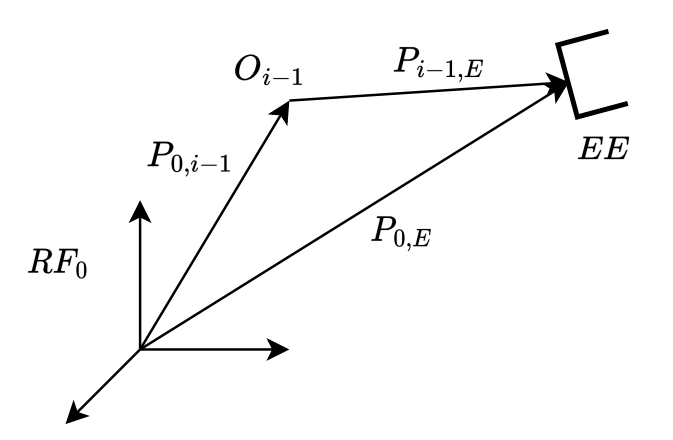
\includegraphics[width=0.75\linewidth]{PosizioneRelativaEE.png}
    \end{minipage}
\end{figure}

\newpage
\subsection{Analisi Della Mobilità Tramite Jacobiano}
Fissata una specifica configurazione dei giunti $\bm{q}$, si può determinare quali movimenti l'end-effector può compiere istantaneamente. Quindi, Per una data configurazione, l'insieme di tutte le velocità che l'end-effector può assumere, è lo \textbf{Spazio Immagine} della matrice Jacobiana, indicato con $R(\bm{J})$. La dimensione di questo spazio, è definita dal rango della matrice, $\rho(\bm{J})$ e a seconda di questo valore possiamo trovarci in due situazioni distinte.

\paragraph{Configurazione Non-Singolare (Rango Pieno)}\mbox{}\\
Una configurazione è non-singolare quando il rango dello Jacobiano è massimo e coincide con la dimensione $m$ dello spazio di lavoro (con $m \le n$, dove $n$ è il numero di giunti). In questo caso, lo spazio delle velocità raggiungibili copre l'intero spazio di lavoro $\mathbb{R}^m$. e quindi il manipolatore gode della massima mobilità. Scegliendo opportunamente le velocità dei giunti, è possibile muovere l'end-effector istantaneamente in qualsiasi direzione desiderata.

\paragraph{Configurazione Singolare (Rango Deficiente)}\mbox{}\\
Una configurazione è singolare se il rango della Jacobiana è inferiore alla dimensione dello spazio di lavoro, ovvero $\rho(\bm{J}) < m$. In questa condizione, lo spazio delle velocità raggiungibili è un sottospazio proprio di $\mathbb{R}^m$ e quindi la mobilità del robot è limitata. Questo significa che esistono delle \textbf{direzioni di moto precluse}, ovvero delle velocità che l'end-effector è istantaneamente incapace di produrre, indipendentemente dalla velocità impressa ai giunti

\subsubsection{Identificare le Direzioni di Moto Precluse}
Attraverso la cinematica differenziale, lo Jacobiano mette in relazione le velocità dei giunti con le velocità lineari e angolari dell'end-effector. Si può scomporre lo spazio delle velocità dell'end-effector in due sottospazi ortogonali e complementari: lo spazio immagine dello Jacobiano $R(\bm{J})$, e lo spazio nullo della sua trasposta, $N(\bm{J}^T)$. Questa scomposizione, espressa dalla relazione:
\[
    \mathbb{R}^m = R(\bm{J}) \oplus N(\bm{J}^T)
\]
Questo significa che ogni vettore di velocità $\dot{\bm{r}}$ nello spazio di lavoro può essere visto unicamente come la somma di una componente in $R(\bm{J})$ e una in $N(\bm{J}^T)$.

Da ciò ne consegue una distinzione netta:
\begin{itemize}
    \item Le \textbf{Direzioni Di Moto Raggiungibili} sono tutte quelle che appartengono allo spazio immagine dello Jacobiano, $R(\bm{J})$. Questo sottospazio è generato dalle combinazioni lineari delle colonne $\bm{J}_{i}$ e rappresenta l'insieme di tutte le velocità che l'end-effector può generare a partire da una specifica configurazione del vettore delle variabili di giunto \(\bm{q}\)
    \item Le \textbf{Direzioni Di Moto Precluse}, sono le direzioni che si trovano nel nucleo della Jacobiana trasposta $N(\bm{J}^T)$. Questo sottospazio è ortogonale a $R(\bm{J})$ e contiene tutte le direzioni di velocità che l'end-effector non è in grado di eseguire in una data configurazione. In pratica, per trovare le direzioni in cui il movimento del robot è bloccato basta calcolare una base per il kernel di $\bm{J}^T$.
\end{itemize}

\subsubsection{Distinzione Fondamentale: Direzioni Precluse e Automovimenti}
È molto importante notare che il concetto di \textit{direzione di moto preclusa} è diverso dal concetto di \textit{automovimento}, in quanto sono due fenomeni diversi e appartengono a sottospazi differenenti.

\begin{itemize}
    \item \textbf{Direzioni di Moto Precluse ($N(\bm{J}^T)$):} Sono \textit{velocità dell'end-effector} che il robot non può fisicamente realizzare. Sono una \textbf{limitazione intrinseca} del manipolatore in una specifica configurazione.

    \item \textbf{Automovimenti ($N(\bm{J})$):} Sono \textit{velocità dei giunti} che, anche se fanno muovere la struttura del robot, \textbf{non producono una variazione della posa dell'end-effector} ($\dot{\bm{r}} = \bm{J}\dot{\bm{q}} = \bm{0}$). Rappresentano una \textbf{capacità aggiuntiva} del robot, tipica dei sistemi ridondanti. Un esempio pratico è la capacità di un braccio robotico con più di sei giunti di riposizionare il gomito per evitare una collisione, il tutto senza che la posa dell'end-effector cambi.
\end{itemize}

% \[
%     \dot{r} \quad       % Velocità
%     \ddot{r} \quad      % Accelerazione
%     \dddot{r} \quad     % Jerk
%     \ddddot{r}          % Snap
% \]

\newpage
\subsection{Esempio: Jacobiano Geometrico Del Robot Planare RR}
In questa sezione si applica il metodo sistematico per il calcolo del Jacobiano geometrico, uno strumento matematico fondamentale che mette in relazione le velocità dei giunti di un robot con le velocità lineari e angolari del suo end-effector. L'analisi è svolta per un robot planare a due giunti rotoidali (RR), come mostrato in figura.

\begin{minipage}[r]{0.25\textwidth}
    \centering
    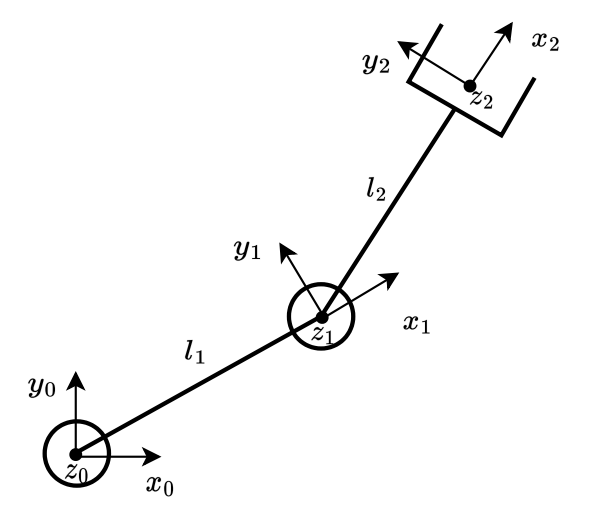
\includegraphics[width=0.99\linewidth]{RobotRRPlanare.png}
\end{minipage}
\hfill
\begin{minipage}[c]{0.73\textwidth}
Il primo passo consiste nel definire le matrici di trasformazione omogenea che descrivono la posizione e l'orientamento di ogni terna solidale ai bracci rispetto alla terna base. Utilizzando la convenzione di Denavit-Hartenberg, si ottengono le seguenti matrici. Per semplicità di notazione, si adotta la forma compatta \(c_i = \cos(q_i)\), \(s_i = \sin(q_i)\), \(c_{ij} = \cos(q_i + q_j)\) e \(s_{ij} = \sin(q_i + q_j)\).
    \[
        \;^{0}{\bm{T}}_0 = \bm{I}_{4 \times 4}
        \quad
        \;^{0}{\bm{T}}_1 =
        \begin{bmatrix}
            c_1 & -s_1 & 0 & l_1 c_1 \\
            s_1 & c_1 & 0 & l_1 s_1 \\
            0 & 0 & 1 & 0 \\
            0 & 0 & 0 & 1
        \end{bmatrix}
        \quad
        \;^{0}{\bm{T}}_2 =
        \begin{bmatrix}
            c_{12} & -s_{12} & 0 & l_1 c_1 + l_2 c_{12} \\
            s_{12} & c_{12} & 0 & l_1 s_1 + l_2 s_{12} \\
            0 & 0 & 1 & 0 \\
            0 & 0 & 0 & 1
        \end{bmatrix}
    \]
    Da queste matrici si estraggono i vettori necessari per costruire le colonne del Jacobiano.
\end{minipage}

Lo Jacobiano \(\bm{J}(\bm{q})\) è una matrice \(6 \times 2\) (poiché l'end-effector si muove nello spazio 3D e il robot ha 2 gradi di libertà) le cui colonne \( \bm{J}_i \) rappresentano il contributo del giunto \(i\)-esimo alla velocità dell'end-effector.

\paragraph{Calcolo Per La Colonna 1 (Giunto 1)}
La prima colonna del Jacobiano, \(\bm{J}_1\), descrive l'effetto della velocità del primo giunto, \(\dot{q}_1\), sulla velocità dell'end-effector. Poiché il giunto 1 è rotoidale, la sua colonna è data da:
\[ \bm{J}_1 = \begin{bmatrix} \bm{J}_{L1} \\ \bm{J}_{A1} \end{bmatrix} = \begin{bmatrix} \bm{z}_0 \times (\bm{p}_{0,e} - \bm{p}_{0,0}) \\ \bm{z}_0 \end{bmatrix} \]
dove \(\bm{z}_0\) è l'asse di rotazione del giunto 1 e \((\bm{p}_{0,e} - \bm{p}_{0,0})\) è il vettore "braccio di leva" che va dall'origine del giunto 1 all'end-effector.

\begin{itemize}
    \item \textbf{Asse di rotazione \(\bm{z}_0\):} Il primo giunto ruota attorno all'asse \(z\) della terna base (terna 0). Questo vettore è quindi per definizione:
    \[ \bm{z}_0 = \begin{bmatrix} 0 \\ 0 \\ 1 \end{bmatrix} \]
    \item \textbf{Vettore Leva \(\bm{p}_{0,e}\):} È il vettore posizione dell'end-effector rispetto alla terna base. Questo vettore si estrae direttamente dalla quarta colonna della matrice di trasformazione totale \(\;^{0}{\bm{T}}_2\). L'origine del giunto 1 coincide con l'origine della terna base, quindi \(\bm{p}_{0,0} = \bm{0}\) e il braccio di leva è semplicemente \(\bm{p}_{0,e}\).
    \[ \bm{p}_{0,e} = \begin{bmatrix} l_1 c_1 + l_2 c_{12} \\ l_1 s_1 + l_2 s_{12} \\ 0 \end{bmatrix} \]
\end{itemize}
Essendo un giunto rotoidale, si applicano le formule per calcolare la parte angolare (\(\bm{J}_{A1}\)) e lineare (\(\bm{J}_{L1}\)) della colonna:
\[
    \bm{J}_{A1} = \bm{z}_0 = \begin{bmatrix} 0 \\ 0 \\ 1 \end{bmatrix}
\]
La parte lineare si ottiene dal prodotto vettoriale tra l'asse di rotazione e il braccio di leva:
\[
    \bm{J}_{L1} = \bm{z}_0 \times \bm{p}_{0,e} =
    \begin{vmatrix}
        \bm{i} & \bm{j} & \bm{k} \\
        0 & 0 & 1 \\
        l_1 c_1 + l_2 c_{12} & l_1 s_1 + l_2 s_{12} & 0
    \end{vmatrix}
    = \begin{bmatrix} -(l_1 s_1 + l_2 s_{12}) \\ l_1 c_1 + l_2 c_{12} \\ 0 \end{bmatrix}
\]

\paragraph{Calcolo per la Colonna 2 (Giunto 2)}
La seconda colonna, \(\bm{J}_2\), descrive l'effetto della velocità del secondo giunto, \(\dot{q}_2\). La formula generale è:
\[ \bm{J}_2 = \begin{bmatrix} \bm{J}_{L2} \\ \bm{J}_{A2} \end{bmatrix} = \begin{bmatrix} \bm{z}_1 \times (\bm{p}_{0,e} - \bm{p}_{0,1}) \\ \bm{z}_1 \end{bmatrix} \]
dove \(\bm{z}_1\) è l'asse di rotazione del giunto 2 e \((\bm{p}_{0,e} - \bm{p}_{0,1})\) è il vettore che congiunge l'origine del giunto 2 con l'end-effector.

\begin{itemize}
    \item \textbf{Asse di rotazione \(\bm{z}_1\):} È l'asse di rotazione del secondo giunto, espresso nelle coordinate della terna base. Si ottiene estraendo la terza colonna della matrice di rotazione \(\prescript{0}{}{\bm{R}}_1\), che è la sottomatrice \(3 \times 3\) in alto a sinistra di \(\prescript{0}{}{\bm{T}}_1\). In questo caso planare, l'asse di rotazione è sempre parallelo all'asse \(z\) globale.
    \[ \bm{z}_1 = \begin{bmatrix} 0 \\ 0 \\ 1 \end{bmatrix} \]
    \item \textbf{Vettore Leva \(\bm{p}_{1,e}\):} È il vettore che va dall'origine del giunto 2 all'end-effector, calcolato come \(\bm{p}_{1,e} = \bm{p}_{0,e} - \bm{p}_{0,1}\). Il vettore \(\bm{p}_{0,1}\) (posizione del giunto 2 rispetto alla base) si trova nella quarta colonna di \(\prescript{0}{}{\bm{T}}_1\).
    \[
        \bm{p}_{1,e} =
        \begin{bmatrix} l_1 c_1 + l_2 c_{12} \\ l_1 s_1 + l_2 s_{12} \\ 0 \end{bmatrix}
        -
        \begin{bmatrix} l_1 c_1 \\ l_1 s_1 \\ 0 \end{bmatrix}
        =
        \begin{bmatrix} l_2 c_{12} \\ l_2 s_{12} \\ 0 \end{bmatrix}
    \]
\end{itemize}
Anche il secondo giunto è rotoidale, quindi si usano le stesse formule:
\[
    \bm{J}_{A2} = \bm{z}_1 = \begin{bmatrix} 0 \\ 0 \\ 1 \end{bmatrix}
\]
\[
    \bm{J}_{L2} = \bm{z}_1 \times \bm{p}_{1,e} =
    \begin{vmatrix}
        \bm{i} & \bm{j} & \bm{k} \\
        0 & 0 & 1 \\
        l_2 c_{12} & l_2 s_{12} & 0
    \end{vmatrix}
    = \begin{bmatrix} -l_2 s_{12} \\ l_2 c_{12} \\ 0 \end{bmatrix}
\]

\paragraph{Jacobiano Geometrico Completo}\(\mbox{}\)\\
Assemblando le colonne calcolate, si ottiene lo Jacobiano geometrico completo. La matrice è strutturata con la parte relativa alla velocità lineare (\(\bm{J}_L\)) nelle prime tre righe e quella relativa alla velocità angolare (\(\bm{J}_A\)) nelle ultime tre.
\[
    \bm{J}(\bm{q}) =
    \begin{bmatrix}
        \bm{J}_{L1} & \bm{J}_{L2} \\
        \bm{J}_{A1} & \bm{J}_{A2}
    \end{bmatrix}
    =
    \begin{bmatrix}
        -l_1 s_1 - l_2 s_{12} & -l_2 s_{12} \\
        l_1 c_1 + l_2 c_{12} & l_2 c_{12} \\
        0 & 0 \\
        \hdashline[2pt/2pt]
        0 & 0 \\
        0 & 0 \\
        1 & 1
    \end{bmatrix}
\]
La relazione tra le velocità dei giunti \(\dot{\bm{q}} = [\dot{q}_1, \dot{q}_2]^T\) e le velocità dell'end-effector \(\bm{\dot{r}}_e = [\bm{v}_e^T, \bm{\omega}_e^T]^T\) è data da \(\bm{\dot{r}}_e = \bm{J}(\bm{q})\dot{\bm{q}}\). Espandendo questa equazione, si ottengono le espressioni per la velocità lineare \(\bm{v}_e\) e angolare \(\bm{\omega}_e\):
\[
    \bm{v}_e =
    \begin{bmatrix} -l_1 s_1 - l_2 s_{12} \\ l_1 c_1 + l_2 c_{12} \\ 0 \end{bmatrix} \dot{q}_1
    +
    \begin{bmatrix} -l_2 s_{12} \\ l_2 c_{12} \\ 0 \end{bmatrix} \dot{q}_2
\]
\[
    \bm{\omega}_e =
    \begin{bmatrix} 0 \\ 0 \\ 1 \end{bmatrix} \dot{q}_1
    +
    \begin{bmatrix} 0 \\ 0 \\ 1 \end{bmatrix} \dot{q}_2
    = \begin{bmatrix} 0 \\ 0 \\ \dot{q}_1 + \dot{q}_2 \end{bmatrix}
\]
Queste equazioni mostrano esplicitamente come la velocità di ciascun giunto contribuisca al moto dell'organo terminale. La velocità angolare totale, ad esempio, è semplicemente la somma delle velocità angolari dei due giunti, come è logico attendersi in un sistema planare.

\newpage
\subsection{Relazione tra Singolarità e Jacobiano}
\subsubsection{Richiami di Algebra Lineare}

La matrice Jacobiana \(\bm{J}\) è lo strumento matematico che crea un ponte tra lo spazio delle velocità dei giunti e lo spazio delle velocità dell'end-effector, secondo la relazione \(\bm{\dot{r}} = \bm{J}(\bm{q})\dot{\bm{q}}\). Le configurazioni in cui un robot perde la capacità di muoversi in certe direzioni, note come singolarità, sono interamente descritte dalle proprietà algebriche della matrice Jacobiana. Analizziamo i concetti fondamentali.

\begin{itemize}
    \item \textbf{Rango di una Matrice:} Data una matrice $\bm{J} \in \mathbb{R}^{m \times n}$, il suo \textit{rango}, denotato con $\rho(\bm{J})$, è il massimo numero di colonne (o righe) linearmente indipendenti. Fisicamente, il rango rappresenta il numero di direzioni indipendenti lungo le quali l'end-effector può muoversi (sia in traslazione che in rotazione). Il rango è sempre limitato dalla dimensione più piccola della matrice:
    \[
        \rho(\bm{J}) \leq \min\{m, n\}
    \]

    \item \textbf{Rango Pieno e Rango Carente:} Si dice che la matrice \(\bm{J}\) ha \textit{rango pieno} quando il suo rango raggiunge il valore massimo possibile, ovvero $\rho(\bm{J}) = \min\{m, n\}$. In questa condizione, il robot ha la massima manovrabilità possibile per la sua struttura. Se, in una certa configurazione \(\bm{q}\), il rango diminuisce, $\rho(\bm{J}) < \min\{m, n\}$, si dice che la matrice è \textit{rango-carente} (o \textit{rank-deficient}), e il robot si trova in una \textbf{singolarità}.

    \item \textbf{Matrice Singolare e Non-Singolare (per matrici quadrate):} Nel caso comune di robot non ridondanti, dove il numero di giunti \(n\) è uguale al numero di gradi di libertà dell'end-effector \(m\), lo Jacobiano è una matrice quadrata ($\bm{J} \in \mathbb{R}^{n \times n}$).
    \begin{itemize}
        \item Una matrice quadrata è detta \textbf{non-singolare} se ha rango pieno ($\rho(\bm{J}) = n$). Questa condizione è equivalente ad affermare che il suo determinante è non nullo ($\det(\bm{J}) \neq 0$) e che esiste la sua unica matrice inversa $\bm{J}^{-1}$, tale che $\bm{J}\bm{J}^{-1} = \bm{J}^{-1}\bm{J} = \bm{I}$. L'invertibilità è cruciale: permette di calcolare in modo univoco le velocità dei giunti \(\dot{\bm{q}}\) necessarie per ottenere una data velocità dell'end-effector \(\bm{\dot{r}}\) tramite la relazione \(\dot{\bm{q}} = \bm{J}^{-1}\bm{\dot{r}}\).
        \item Una matrice quadrata è detta \textbf{singolare} se non è invertibile. Ciò accade precisamente quando la matrice è rango-carente ($\rho(\bm{J}) < n$), ovvero quando il suo determinante è nullo. In una configurazione singolare, il robot perde uno o più gradi di libertà e non è più possibile mappare univocamente le velocità cartesiane a quelle dei giunti.
    \end{itemize}

    \item \textbf{Immagine (o Spazio delle Colonne):} L'\textit{immagine} di \(\bm{J}\), indicata con $R(\bm{J})$, è il sottospazio vettoriale generato dalle colonne di \(\bm{J}\). In termini pratici, rappresenta l'insieme di \textbf{tutte le possibili velocità dell'end-effector} \(\bm{\dot{r}}\) che il robot può generare.
    \[
        R(\bm{J}) = \{\bm{\dot{r}} \in \mathbb{R}^{m} \mid \exists \dot{\bm{q}} \in \mathbb{R}^{n} \text{ tale che } \bm{\dot{r}} = \bm{J}\dot{\bm{q}}\}
    \]
    La dimensione di questo sottospazio è esattamente il rango della matrice:
    \[
        \dim(R(\bm{J})) = \rho(\bm{J})
    \]
    Quando il robot entra in una singolarità, il rango \(\rho(\bm{J})\) diminuisce, e con esso si "restringe" lo spazio delle velocità raggiungibili dall'end-effector.

    \item \textbf{Nucleo (o Spazio Nullo):} Il \textit{nucleo} di \(\bm{J}\), indicato con $N(\bm{J})$, è il sottospazio dei vettori di velocità dei giunti \(\dot{\bm{q}}\) che producono una velocità nulla dell'end-effector.
    \[
        N(\bm{J}) = \{\dot{\bm{q}} \in \mathbb{R}^{n} \mid \bm{J}\dot{\bm{q}} = \bm{0}\}
    \]
    Un nucleo non banale (cioè che non contiene solo il vettore nullo) implica l'esistenza di \textbf{movimenti interni} dei giunti che non modificano la posa dell'end-effector. Questo fenomeno è la base della \textbf{ridondanza} nei robot.
    \newpage
    \item \textbf{Teorema Rango-Nullità:} Questo teorema fondamentale lega le dimensioni dell'immagine e del nucleo al numero di giunti \(n\) (la dimensione dello spazio di partenza):
    \[
        \dim(R(\bm{J})) + \dim(N(\bm{J})) = n
    \]
    Sostituendo $\dim(R(\bm{J})) = \rho(\bm{J})$, si ottiene:
    \[
        \dim(N(\bm{J})) = n - \rho(\bm{J})
    \]
    Questa relazione ci dice che se il rango diminuisce (singolarità), la dimensione dello spazio nullo aumenta. Anche per un robot non ridondante, in una singolarità compare un nucleo non banale, che si manifesta come un moto istantaneo dei giunti che non produce movimento dell'end-effector.

    \item \textbf{Sottospazi Fondamentali e Decomposizione Ortogonale:} Per una comprensione completa della trasformazione operata da \(\bm{J}\), si analizzano i quattro sottospazi fondamentali: l'immagine \(R(\bm{J})\), il nucleo \(N(\bm{J})\), e i corrispondenti spazi per la sua trasposta, \(R(\bm{J}^T)\) e \(N(\bm{J}^T)\). Questi sottospazi permettono di decomporre gli spazi di partenza (velocità dei giunti, \(\mathbb{R}^n\)) e di arrivo (velocità dell'end-effector, \(\mathbb{R}^m\)) in componenti ortogonali.
    \[
    \begin{cases}
        R(\bm{J}) \oplus N(\bm{J}^T) = \mathbb{R}^{m} \\
        R(\bm{J}^T) \oplus N(\bm{J}) = \mathbb{R}^{n}
    \end{cases}
    \]
    Il simbolo \(\oplus\) denota la \textit{somma diretta}, che implica che ogni vettore dello spazio può essere scritto in modo \textbf{unico} come somma di un vettore da ciascun sottospazio.

    La seconda relazione, $R(\bm{J}^T) \oplus N(\bm{J}) = \mathbb{R}^{n}$, è particolarmente significativa:
    \begin{itemize}
        \item Lo spazio \(R(\bm{J}^T)\) è l'insieme delle velocità dei giunti che sono "efficienti", ovvero che producono un movimento dell'end-effector.
        \item Lo spazio \(N(\bm{J})\) è l'insieme delle velocità dei giunti che corrispondono a moti interni (inefficienti dal punto di vista del movimento dell'end-effector).
    \end{itemize}
    Questa decomposizione ci dice che qualsiasi vettore di velocità dei giunti \(\dot{\bm{q}}\) può essere scomposto in modo univoco in una componente che muove l'end-effector e una che non lo fa.
\end{itemize}


\newpage
\subsection{Spazio Dei Giunti E Spazio Dei Compiti}
Nell'analisi cinematica è fondamentale la matrice Jacobiana, indicata con $\bm{J}$, che non è una matrice costante. Infatti, dipende dalla configurazione del robot, la quale è descritta dal vettore delle variabili di giunto $\bm{q}$. Questa dipendenza implica che tutte le proprietà fondamentali dello Jacobiano come il rango $\rho$, lo spazio immagine $R$, e il nucleo $N$ siano proprietà \textit{locali}, che variano al variare di $\bm{q}$:
\[
    \rho(\bm{J}) = \rho(\bm{J}(\bm{q})), \quad R(\bm{J}) = R(\bm{J}(\bm{q})), \quad N(\bm{J}) = N(\bm{J}(\bm{q}))
\]
La relazione cinematica differenziale, espressa dall'equazione $\bm{v} = \bm{J}(\bm{q})\dot{\bm{q}}$, fornisce la chiave per dare un'interpretazione fisica diretta a questi sottospazi matematici.

\begin{center}
    \resizebox{0.75\linewidth}{!}{%
        \begin{tikzpicture}
            % Cerchio centrato in un punto
            \draw (2,2) circle (1.75cm);
            \draw (2,2) circle (1cm);

            \draw (10,2) circle (1.75cm);
            \draw (10,2) circle (1cm);

            % Punto definito con coordinate
            \filldraw[black] (1.75,2.25) circle (1.5pt);
            \node at (1.75,2.5) {$\bm{0}$};

            \filldraw[black] (10,2.25) circle (1.5pt);
            \node at (10,2.5) {$\bm{0}$};

            % Linea che collega due punti
            \draw (2, 3.75) -- (10, 3);
            \draw (2, 0.25) -- (10, 1);

            \draw (2, 3) -- (10,2.25);
            \draw (2, 1) -- (10,2.25);

            % Etichette
            \node at (2,1.5) {$N(J)$};
            \node at (10,1.5) {$R(J)$};
        \end{tikzpicture}
    }
\end{center}

\begin{itemize}
    \item \textbf{Spazio Velocità Raggiungibili:} Lo spazio immagine dello Jacobiano, $R(\bm{J}(\bm{q}))$, noto anche come \textit{spazio delle velocità generalizzate}, rappresenta l'intero insieme di velocità (sia lineari che angolari) che l'end-effector è in grado di raggiungere in una specifica configurazione $\bm{q}$. Questo spazio si ottiene considerando tutte le possibili combinazioni di velocità dei giunti $\dot{\bm{q}}$. Quando il rango della matrice è massimo e coincide con la dimensione dello spazio dei compiti ($m$), ovvero $\rho(\bm{J}(\bm{q})) = m$, il robot gode della massima manovrabilità e quindi l'end-effector può muoversi istantaneamente in qualsiasi direzione dello spazio operativo $\mathbb{R}^{m}$.

    \item \textbf{Direzioni Di Moto Precluse:} Quando, in una data configurazione $\bm{q}$, il rango dello Jacobiano scende al di sotto della dimensione dello spazio dei compiti ($\rho(\bm{J}(\bm{q})) < m$), emergono delle limitazioni. In queste condizioni, esistono delle direzioni nello spazio operativo $\mathbb{R}^{m}$ lungo le quali l'end-effector non può muoversi, indipendentemente dalla velocità dei giunti. Queste direzioni "proibite" sono definite dal sottospazio $N(\bm{J}^T(\bm{q}))$. Una configurazione che presenta questa perdita di mobilità è definita \textit{configurazione singolare} o, più semplicemente, \textit{singolarità}.

    \item \textbf{Automovimenti:} Se lo spazio nullo dello Jacobiano, $N(\bm{J}(\bm{q}))$, non è banale, cioè se contiene vettori non nulli, allora è fisicamente possibile avere combinazioni di velocità dei giunti non nulle ($\dot{\bm{q}} \neq \bm{0}$) che producono una velocità dell'end-effector pari a zero ($\bm{v} = \bm{0}$). Questi movimenti, che modificano la configurazione interna del robot senza spostare l'end-effector, sono chiamati \textit{automovimenti}. Questa caratteristica è tipica dei \textit{robot ridondanti}, ovvero quei robot in cui il numero di giunti è maggiore della dimensione dello spazio dei compiti ($n > m$). Per tali sistemi, la condizione $N(\bm{J}(\bm{q})) \neq \{\bm{0}\}$ è sempre verificata.
\end{itemize}

\newpage
\subsection{Analisi della Mobilità nello Spazio dei Compiti: Robot RRR Planare}
Si consideri un manipolatore planare composto da tre giunti rotoidali (configurazione RRR). Per semplificare i calcoli, assumiamo che tutti i bracci abbiano la stessa lunghezza, pari a uno: $l_1 = l_2 = l_3 = 1$.

Il compito che vogliamo assegnare a questo robot è il controllo della \textbf{posizione} dell' end-effector nel piano $xy$. Tale posizione è descritta dal vettore $\bm{r} = [x, y]^T$. Lo spazio in cui il compito è definito (lo "spazio dei compiti") ha quindi dimensione $m=2$. D'altra parte, il robot è descritto da tre variabili di giunto indipendenti ($q_1, q_2, q_3$), per cui il suo spazio di configurazione (o "spazio dei giunti") ha dimensione $n=3$.

Poiché il numero di gradi di libertà del robot ($n=3$) è maggiore del numero di gradi di libertà richiesti per eseguire il compito ($m=2$), il robot è definito \textbf{ridondante} rispetto a questo specifico compito. Ciò significa che esistono infinite configurazioni dei giunti che permettono all'end-effector di raggiungere la stessa posizione nel piano.

Lo spazio di lavoro del manipolatore, ovvero l'insieme di tutti i punti raggiungibili dall'end-effector, è una corona circolare. Il raggio esterno di 3 (unità) si ottiene quando tutti i bracci sono completamente estesi in linea retta, mentre il raggio interno di 1 (unità) si ha quando il secondo e il terzo braccio sono ripiegati sul primo.

\begin{figure}[h!]
    \centering
    \begin{minipage}[b]{0.45\textwidth}
        \centering
        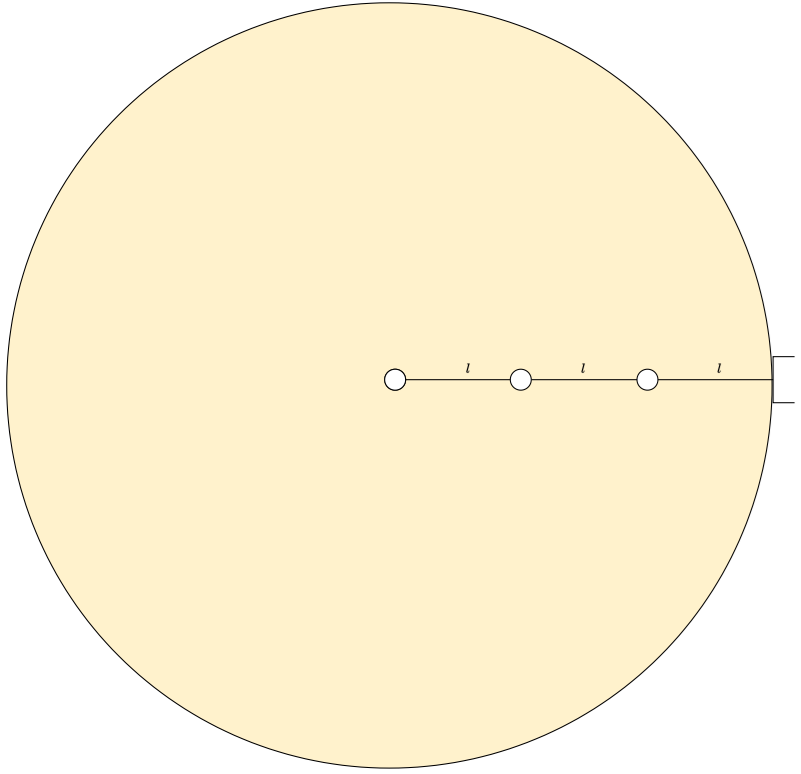
\includegraphics[width=0.7\linewidth]{SpazioOperativoPrimario.png}
        \caption{Spazio Operativo Primario (Raggio 3)}
    \end{minipage}
    \hfill
    \begin{minipage}[b]{0.45\textwidth}
        \centering
        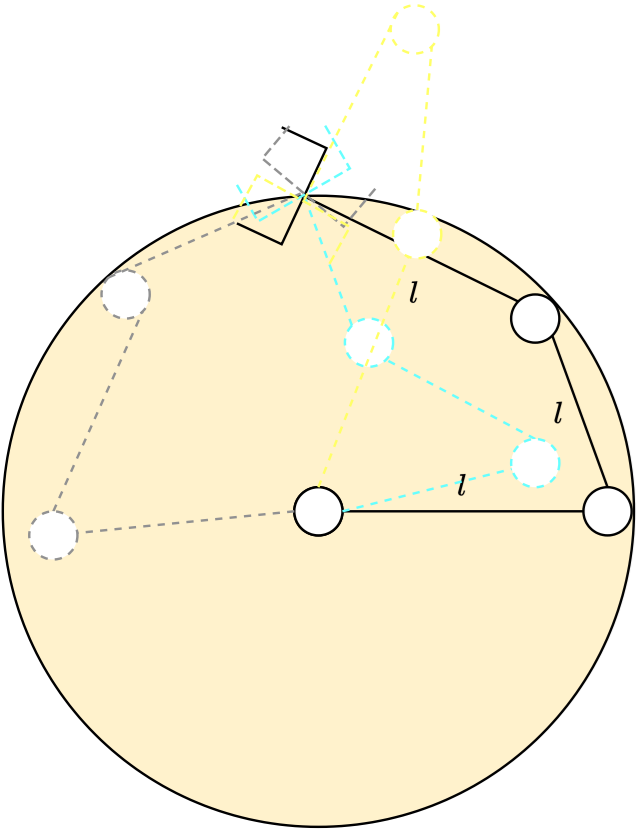
\includegraphics[width=0.65\linewidth]{SpazioOperativoSecondario.png}
        \caption{Spazio Operativo Secondario (Raggio 1)}
    \end{minipage}
\end{figure}

\paragraph{Passo 1: Cinematica Diretta e Matrici di Trasformazione.}
Il primo passo per poter analizzare la mobilità del robot è derivare il suo modello cinematico diretto. Come sappiamo, si deve calcolare la funzione matematica che ci fornisce la posizione (e l'orientamento) dell'end-effector a partire da una data configurazione del vettore delle variabili di giunto $\bm{q} = [q_1, q_2, q_3]^T$. Per ottenere questo modello, utilizziamo la \textbf{convenzione di Denavit-Hartenberg (DH)}. I parametri DH per il nostro manipolatore RRR planare sono riportati nella tabella:.

\begin{table}[h!]
    \centering
    \begin{tabular}{|c|cccc|}
        \hline
        \textbf{Braccio} & $\boldsymbol{\theta_i}$ & $\boldsymbol{d_i}$ & $\boldsymbol{\alpha_i}$ & $\boldsymbol{a_i}$ \\
        \hline
        1 & $q_{1}$ & 0 & 0 & $l_1=1$ \\
        2 & $q_{2}$ & 0 & 0 & $l_2=1$ \\
        3 & $q_{3}$ & 0 & 0 & $l_3=1$ \\
        \hline
    \end{tabular}
\end{table}

Sostituendo questi parametri nella matrice di trasformazione omogenea standard, si ottengono le matrici che descrivono la posa (posizione e orientamento) di ogni terna di riferimento solidale a un braccio rispetto alla terna precedente.
\newpage
Data la semplicità della cinematica planare e la scelta dei parametri DH, le matrici sono:
\[
    {}^0\bm{A}_1(q_1) =
    \begin{bmatrix}
        c_1 & -s_1 & 0 & c_1 \\
        s_1 & c_1 & 0 & s_1 \\
        0 & 0 & 1 & 0 \\
        0 & 0 & 0 & 1
    \end{bmatrix} \! , \quad
    {}^1\bm{A}_2(q_2) =
    \begin{bmatrix}
        c_2 & -s_2 & 0 & c_2 \\
        s_2 & c_2 & 0 & s_2 \\
        0 & 0 & 1 & 0 \\
        0 & 0 & 0 & 1
    \end{bmatrix} \! , \quad
    {}^2\bm{A}_3(q_3) =
    \begin{bmatrix}
        c_3 & -s_3 & 0 & c_3 \\
        s_3 & c_3 & 0 & s_3 \\
        0 & 0 & 1 & 0 \\
        0 & 0 & 0 & 1
    \end{bmatrix}
\]
Dove, per compattezza, si adotta la notazione $c_i = \cos(q_i)$ e $s_i = \sin(q_i)$.

La posa completa dell'end-effector (terna $\{3\}$) rispetto alla base del robot (terna $\{0\}$) si ottiene componendo queste trasformazioni, ovvero moltiplicando le matrici singole: ${}^0\bm{A}_3(\bm{q}) = {}^0\bm{A}_1(q_1) {}^1\bm{A}_2(q_2) {}^2\bm{A}_3(q_3)$. Il risultato di questo prodotto è:
\[
    {}^0\bm{A}_3(\bm{q}) =
    \begin{bmatrix}
        c_{123} & -s_{123} & 0 & c_1 + c_{12} + c_{123} \\
        s_{123} & c_{123} & 0 & s_1 + s_{12} + s_{123} \\
        0 & 0 & 1 & 0 \\
        0 & 0 & 0 & 1
    \end{bmatrix}
\]
Dove si è usata la notazione $c_{12} = \cos(q_1+q_2)$, $s_{123} = \sin(q_1+q_2+q_3)$. La quarta colonna di questa matrice rappresenta il vettore posizione dell'origine della terna $\{3\}$ rispetto alla terna $\{0\}$. Poiché il nostro compito riguarda solo la posizione planare, estraiamo le prime due componenti di questo vettore per ottenere la funzione di cinematica diretta che ci interessa:
\[
    \bm{r}(\bm{q}) =
    \begin{bmatrix} x(\bm{q}) \\ y(\bm{q}) \end{bmatrix} =
    \begin{bmatrix}
        c_1 + c_{12} + c_{123} \\
        s_1 + s_{12} + s_{123}
    \end{bmatrix}
\]

\paragraph{Passo 2: Calcolo del Jacobiano Geometrico.}
Lo Jacobiano è una matrice che lega le velocità nello spazio dei giunti ($\dot{\bm{q}}$) alle velocità nello spazio dei compiti. In particolare, il \textbf{Jacobiano geometrico} $\bm{J}(\bm{q}) \in \mathbb{R}^{6 \times 3}$ mappa le velocità angolari dei tre giunti alla velocità spaziale dell'end-effector, composta da un vettore di velocità lineare $\bm{v} \in \mathbb{R}^3$ e un vettore di velocità angolare $\bm{\omega} \in \mathbb{R}^3$.

La sua struttura si costruisce colonna per colonna, dove ogni colonna $\bm{J}_i$ rappresenta il contributo del giunto $i$-esimo alla velocità dell'end-effector. Per i giunti rotoidali, la formula è:
\[
\bm{J}_i =
\begin{bmatrix} \bm{J}_{Li} \\ \bm{J}_{Ai} \end{bmatrix} =
\begin{bmatrix} \bm{z}_{i-1} \times (\bm{p}_E - \bm{p}_{i-1}) \\ \bm{z}_{i-1} \end{bmatrix}
\]
Dove:
\begin{itemize}
    \item $\bm{z}_{i-1}$: È il versore che indica l'asse di rotazione del giunto $i$.
    \item $(\bm{p}_E - \bm{p}_{i-1})$: È il vettore che va dall'origine del giunto $i$ alla punta dell'end-effector (il "braccio di leva").
\end{itemize}

Dato che il nostro è un robot planare, tutti i giunti ruotano attorno ad assi paralleli all'asse $z$ del sistema di riferimento base. Pertanto, i vettori degli assi di rotazione sono costanti e uguali:
\[
    \bm{z}_0 = \bm{z}_1 = \bm{z}_2 = \begin{bmatrix} 0 & 0 & 1 \end{bmatrix}^T
\]
Per calcolare i vettori "braccio di leva", dobbiamo trovare le posizioni delle origini dei sistemi di riferimento di ciascun giunto ($\bm{p}_0, \bm{p}_1, \bm{p}_2$) e la posizione dell'end-effector ($\bm{p}_E$). Queste possono essere estratte dalle matrici di trasformazione parziali:
\[
\begin{aligned}
    % Leva Giunto 1
    \bm{p}_{0,E} &= \bm{p}_E - \bm{p}_0 = \begin{bmatrix} x \\ y \\ 0 \end{bmatrix} - \begin{bmatrix} 0 \\ 0 \\ 0 \end{bmatrix} = \begin{bmatrix} c_1+c_{12}+c_{123} \\ s_1+s_{12}+s_{123} \\ 0 \end{bmatrix} \\
    % Leva Giunto 2
    \bm{p}_{1,E} &= \bm{p}_E - \bm{p}_1 = \begin{bmatrix} x \\ y \\ 0 \end{bmatrix} - \begin{bmatrix} c_1 \\ s_1 \\ 0 \end{bmatrix} = \begin{bmatrix} c_{12}+c_{123} \\ s_{12}+s_{123} \\ 0 \end{bmatrix} \\
    % Leva Giunto 3
    \bm{p}_{2,E} &= \bm{p}_E - \bm{p}_2 = \begin{bmatrix} x \\ y \\ 0 \end{bmatrix} - \begin{bmatrix} c_1+c_{12} \\ s_1+s_{12} \\ 0 \end{bmatrix} = \begin{bmatrix} c_{123} \\ s_{123} \\ 0 \end{bmatrix}
\end{aligned}
\]
Procediamo ora con il calcolo esplicito delle colonne del Jacobiano tramite il prodotto vettoriale:
\[
\begin{alignedat}{2}
    % Colonna 1
    \bm{J}_{L1} &= \bm{z}_0 \times \bm{p}_{0,E} = \begin{bmatrix} -(s_1+s_{12}+s_{123}) \\ c_1+c_{12}+c_{123} \\ 0 \end{bmatrix} &\quad \bm{J}_{A1} &= \bm{z}_0 = \begin{bmatrix} 0 \\ 0 \\ 1 \end{bmatrix} \\
    % Colonna 2
    \bm{J}_{L2} &= \bm{z}_1 \times \bm{p}_{1,E} = \begin{bmatrix} -(s_{12}+s_{123}) \\ c_{12}+c_{123} \\ 0 \end{bmatrix} &\quad \bm{J}_{A2} &= \bm{z}_1 = \begin{bmatrix} 0 \\ 0 \\ 1 \end{bmatrix} \\
    % Colonna 3
    \bm{J}_{L3} &= \bm{z}_2 \times \bm{p}_{2,E} = \begin{bmatrix} -s_{123} \\ c_{123} \\ 0 \end{bmatrix} &\quad \bm{J}_{A3} &= \bm{z}_2 = \begin{bmatrix} 0 \\ 0 \\ 1 \end{bmatrix}
\end{alignedat}
\]
Assemblando queste colonne, otteniamo lo Jacobiano geometrico completo $6 \times 3$:
\[
    \bm{J}(\bm{q}) =
    \begin{bmatrix}
        % Righe velocità lineari (vx, vy, vz)
        -(s_{1} + s_{12} + s_{123}) & -(s_{12} + s_{123}) & -s_{123} \\
        c_{1} + c_{12} + c_{123} & c_{12} + c_{123} & c_{123} \\
        0 & 0 & 0 \\
        \hline
        % Righe velocità angolari (wx, wy, wz)
        0 & 0 & 0 \\
        0 & 0 & 0 \\
        1 & 1 & 1
    \end{bmatrix}
\]

\paragraph{Passo 3: Dal Jacobiano Geometrico al Jacobiano Analitico}
Lo Jacobiano geometrico descrive l'intera velocità spaziale dell'end-effector. Tuttavia, il nostro compito è stato definito in modo più semplice: controllare solo la posizione planare $\bm{r} = [x, y]^T$. Non siamo interessati né alla velocità lungo l'asse $z$ (che è sempre nulla per un robot planare), né alla velocità angolare.

Pertanto, per i nostri scopi, possiamo estrarre dallo Jacobiano geometrico solo le righe che ci interessano, ovvero quelle che corrispondono alle velocità $\dot{x}$ (prima riga) e $\dot{y}$ (seconda riga). Questo processo ci fornisce lo \textbf{Jacobiano di Posizione} $\bm{J}_r(\bm{q}) \in \mathbb{R}^{2 \times 3}$, una matrice che lega direttamente le velocità dei giunti alla velocità cartesiana dell'end-effector nel piano, secondo la relazione fondamentale: $\dot{\bm{r}} = \bm{J}_r(\bm{q})\dot{\bm{q}}$.

Vale la pena notare che si sarebbe potuto ottenere lo stesso risultato derivando direttamente la funzione di posizione $\bm{r}(\bm{q})$ rispetto al vettore dei giunti $\bm{q}$:
\[
    \bm{J}_r(\bm{q}) = \frac{\partial \bm{r}(\bm{q})}{\partial \bm{q}} =
    \begin{bmatrix}
        \frac{\partial x}{\partial q_1} & \frac{\partial x}{\partial q_2} & \frac{\partial x}{\partial q_3} \\
        \frac{\partial y}{\partial q_1} & \frac{\partial y}{\partial q_2} & \frac{\partial y}{\partial q_3}
    \end{bmatrix}
    =
    \begin{bmatrix}
        -(s_{1} + s_{12} + s_{123}) & -(s_{12} + s_{123}) & -s_{123} \\
        c_{1} + c_{12} + c_{123} & c_{12} + c_{123} & c_{123}
    \end{bmatrix}
\]
Questa matrice finale, di dimensioni $2 \times 3$, è lo strumento analitico cruciale che ci permetterà di studiare le configurazioni singolari del robot. Le singolarità si verificano in quelle configurazioni di giunti $\bm{q}$ in cui il rango di $\bm{J}_r$ scende al di sotto del suo valore massimo (che in questo caso è 2), indicando che il robot perde la capacità di muovere il suo end-effector in una o più direzioni del piano.

\newpage
\paragraph{Analisi di Caso 1: Robot Ripiegato (Configurazione Non Singolare)}
\mbox{}\\ % Forza l'inizio di una nuova linea
Per comprendere il significato pratico del Jacobiano, iniziamo analizzando una configurazione specifica e intuitivamente robusta: $\bm{q}_1 = [0, \pi/2, -\pi/2]^T$. Come mostra la figura, in questa posa il robot è parzialmente ripiegato su se stesso, lontano dai limiti del suo spazio di lavoro.

\begin{minipage}[b]{0.33\textwidth}
    \centering
    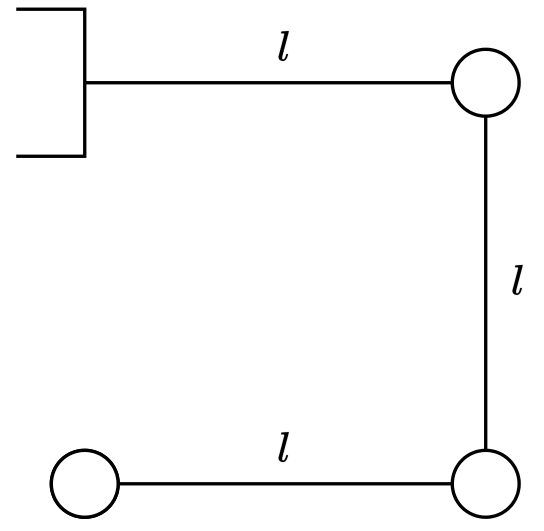
\includegraphics[width=0.75\linewidth]{ConfigurazioneQ1.png}
\end{minipage}
\hfill
\begin{minipage}[b]{0.65\textwidth}
    Per prima cosa, calcoliamo lo Jacobiano in questa configurazione sostituendo i valori degli angoli nella matrice $\bm{J}_r(\bm{q})$ che abbiamo derivato in precedenza. Otteniamo:
    \[
        \bm{J}_r(\bm{q}_1) =
        \begin{bmatrix}
            -1 & -1 & 0 \\
            0 & -1 & -1
        \end{bmatrix}
    \]
\end{minipage}

L'analisi algebrica di questa matrice ci fornisce un quadro completo della mobilità del robot.

\subparagraph{Rango e Spazio Immagine (Direzioni Moto Possibili)}
Il rango della matrice \(\bm{J}_r(\bm{q}_i)\) ci dice quante direzioni indipendenti può generare e siccome è una matrice $2 \times 3$, il rango massimo è 2. Osservando $\bm{J}_r(\bm{q}_1)$, si nota che le prime due colonne, $\begin{bmatrix}-1 \\ 0\end{bmatrix}$ e $\begin{bmatrix}-1 \\ -1\end{bmatrix}$, non sono proporzionali, e quindi sono linearmente indipendenti. Questo è sufficiente per affermare che il rango della matrice è il massimo possibile: $\rho(\bm{J}_r(\bm{q}_1)) = 2$.

Poiché il rango è uguale alla dimensione dello spazio del compito ($m=2$), la matrice ha \textbf{rango pieno}. Questo, per definizione, significa che la configurazione \textbf{non è singolare}.
Lo spazio immagine $R(\bm{J}_r(\bm{q}_1))$, che è l'insieme di tutte le velocità dell'end-effector che possono essere generate, è lo spazio generato dalle colonne della matrice. Poiché abbiamo due colonne linearmente indipendenti in uno spazio 2D, esse generano l'intero piano:
\[
    R(\bm{J}_r(\bm{q}_1)) = \mathrm{span}\left\{
    \begin{bmatrix} -1 \\ 0 \end{bmatrix},
    \begin{bmatrix} -1 \\ -1 \end{bmatrix},
    \begin{bmatrix} 0 \\ -1 \end{bmatrix}
    \right\} = \mathbb{R}^{2}
\]
In questa configurazione, il robot gode della massima mobilità. Qualunque direzione di movimento si desideri per l'end-effector nel piano, esiste una combinazione di velocità dei giunti in grado di produrla.

\subparagraph{Nucleo e Automovimenti (Moti Interni).}
Poiché il robot è ridondante ($n=3 > m=2$), ci aspettiamo di poter muovere i giunti senza che l'end-effector si sposti. Il \textbf{nucleo} (o spazio nullo) dello Jacobiano, $N(\bm{J}_r)$, descrive esattamente questi movimenti. Il teorema rango-nullità ci dice la sua dimensione: $\dim(N(\bm{J}_r)) = n - \rho = 3 - 2 = 1$.
Ciò significa che esiste un'unica "direzione" fondamentale di movimento nello spazio dei giunti che risulta in una velocità nulla dell'end-effector. Questo sottospazio è generato dal vettore:
\[
    N(\bm{J}_r(\bm{q}_1)) = \mathrm{span}\left\{ \begin{bmatrix} 1 \\ -1 \\ 1 \end{bmatrix} \right\}
\]
Questo vettore descrive un \textit{automovimento}. Se imponiamo una velocità dei giunti proporzionale a questo vettore, ad esempio $\dot{\bm{q}} = [k, -k, k]^T$ per una qualsiasi costante $k \neq 0$, i bracci del robot si riconfigureranno internamente, ma la punta dell'end-effector rimarrà istantaneamente ferma. Questa è la diretta manifestazione della ridondanza del manipolatore.

\newpage

\paragraph{Analisi di Caso 2: Robot Esteso (Singolarità di Bordo)}
\mbox{}\\
Consideriamo ora uno scenario completamente diverso: la configurazione $\bm{q}_2 = [0, 0, 0]^T$. Questa posa corrisponde a un robot completamente esteso lungo l'asse x, al limite del suo spazio di lavoro.

\begin{minipage}[c]{0.33\textwidth}
    \centering
    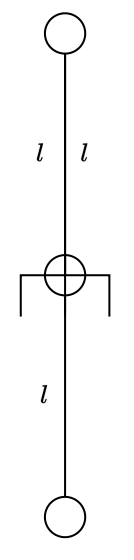
\includegraphics[width=0.25\linewidth]{ConfigurazioneQ2.png}
\end{minipage}
\hfill
\begin{minipage}[c]{0.65\textwidth}
    Sostituendo questi valori nel Jacobiano, otteniamo una matrice dall'aspetto molto differente:
    \[
        \bm{J}_r(\bm{q}_2) =
        \begin{bmatrix}
            0 & 0 & 0 \\
            3 & 2 & 1
        \end{bmatrix}
    \]
\end{minipage}

L'analisi di questa matrice rivela immediatamente una drastica perdita di mobilità.

\subparagraph{Rango e Spazio Immagine}
A colpo d'occhio, notiamo che la prima riga della matrice è nulla. Questo implica che la componente $\dot{x}$ della velocità dell'end-effector sarà sempre zero, indipendentemente dalle velocità dei giunti. Inoltre, tutte le colonne sono chiaramente multipli del vettore $\begin{bmatrix}0 \\ 1\end{bmatrix}$, e quindi sono linearmente dipendenti. Il rango della matrice è quindi $\rho(\bm{J}_r(\bm{q}_2)) = 1$.

Poiché il rango è strettamente minore della dimensione dello spazio del compito ($\rho < m$), la configurazione \textbf{è singolare}. Lo spazio delle velocità possibili non è più un piano, ma degenera in una linea:
\[
    R(\bm{J}_r(\bm{q}_2)) = \mathrm{span}\left\{ \begin{bmatrix} 0 \\ 1 \end{bmatrix} \right\}
\]
Il robot ha perso un grado di libertà operativo. In questa configurazione, l'end-effector può muoversi istantaneamente solo lungo l'asse $y$ (direzione verticale). È diventato \textbf{impossibile} generare una velocità lungo la direzione radiale (l'asse $x$), che è proprio la direzione di allineamento dei bracci. Questo tipo di singolarità, che si verifica ai confini dello spazio di lavoro, è comunemente detta \textbf{singolarità di bordo}.

\subparagraph{Nucleo}
Con la perdita di mobilità esterna, il robot guadagna mobilità interna. La dimensione dello spazio nullo aumenta: $\dim(N(\bm{J}_r(\bm{q}_2))) = n - \rho = 3 - 1 = 2$. Questo significa che ora esistono due direzioni di automovimento linearmente indipendenti; ci sono più modi per muovere i giunti mantenendo l'end-effector fermo.

\paragraph{Conclusioni Analisi}
\mbox{}\\ % Forza l'inizio di una nuova linea
Questa analisi su due semplici configurazioni dimostra il potente ruolo diagnostico del Jacobiano. L'algebra matriciale ci permette non solo di etichettare una posa come "singolare" o "non singolare", ma ci offre una profonda comprensione geometrica e quantitativa della mobilità del manipolatore in ogni istante. Lo \textbf{spazio immagine} definisce l'universo delle velocità raggiungibili dall'end-effector, mentre il \textbf{nucleo} caratterizza la ricchezza dei moti interni (automovimenti) che non influenzano il compito, una caratteristica intrinseca dei sistemi ridondanti.

\newpage
\subsection{Cinematica Differenziale Inversa}
Il problema della cinematica inversa, ovvero la determinazione delle variabili di giunto \(\bm{q}\) a partire da una data posa dell'end-effector, è intrinsecamente complesso a causa della non linearità delle sue equazioni. Un approccio alternativo e più gestibile consiste nell'operare a livello di velocità attraverso la cinematica differenziale. La relazione fondamentale, \(\bm{v}_e = \bm{J}(\bm{q})\dot{\bm{q}}\), stabilisce una trasformazione \textbf{lineare} tra il vettore delle velocità dei giunti \(\dot{\bm{q}}\) e quello delle velocità dell'end-effector \(\bm{v}_e\) per una configurazione \(\bm{q}\) nota. L'obiettivo diventa quindi calcolare le velocità dei giunti \(\dot{\bm{q}}(t)\) necessarie per tracciare una desiderata traiettoria di velocità dell'end-effector \(\bm{v}_e(t)\).

Nel caso ideale di un manipolatore \textbf{non-ridondante} (\(n=m\)), dove il numero di giunti \(n\) eguaglia la dimensione \(m\) dello spazio del compito, la matrice Jacobiana \(\bm{J}(\bm{q})\) è quadrata. Se il robot opera lontano da configurazioni singolari, la Jacobiana ha rango pieno ed è \textbf{invertibile}. In queste circostanze, la soluzione è ottenuta tramite una semplice inversione algebrica:
\[
    \dot{\bm{q}}(t) = \bm{J}^{-1}(\bm{q}(t)) \cdot \bm{v}_e(t)
\]
La traiettoria delle posizioni \(\bm{q}(t)\) può essere poi ricostruita per integrazione numerica. Ad esempio, con il \textbf{metodo di Eulero (In Avanti)}, la posizione al passo successivo è approssimata come \(\bm{q}(t_{k+1}) \approx \bm{q}(t_k) + \dot{\bm{q}}(t_k) \cdot \Delta t\), dove \(\Delta t\) è l'intervallo di tempo.

Tuttavia, l'applicabilità di questo approccio diretto è  limitata, poiché fallisce in due situazioni comuni e critiche. La prima riguarda i \textbf{manipolatori ridondanti} (\(n > m\)), dove la Jacobiana è una matrice rettangolare \(m \times n\) non invertibile, il che implica l'esistenza di infinite soluzioni \(\dot{\bm{q}}\) per la stessa \(\bm{v}_e\). La seconda si verifica in corrispondenza di \textbf{singolarità cinematiche} (\(\rho(\bm{J}) < m\)), configurazioni in cui la Jacobiana perde di rango (\(\det(\bm{J}) = 0\)) e la sua inversa non esiste, portando a velocità di giunto teoricamente infinite.

Per superare questi limiti e formulare una soluzione generale, si ricorre alla \textbf{\textit{Pseudo-Inversa di Moore-Penrose}}, denotata con \(\bm{J}^{\dagger}\). Questo strumento estende il concetto di inversa a matrici di qualsiasi dimensione, anche singolari, garantendo una soluzione al sistema lineare \(\bm{J}\dot{\bm{q}} = \bm{v}_e\) con importanti proprietà di ottimalità. La pseudo-inversa \(\bm{J}^\dagger\) è l'unica matrice che soddisfa le quattro condizioni di Penrose e la sua forma analitica dipende dalle proprietà di \(\bm{J}\):
\begin{itemize}
    \item Se \(\bm{J}\) è quadrata e non singolare, la pseudo-inversa coincide con l'inversa classica: \(\bm{J}^\dagger = \bm{J}^{-1}\).
    \item Per un robot ridondante (\(n > m\)) con Jacobiana a rango pieno (\(\rho(\bm{J}) = m\)), si utilizza la \textbf{pseudo-inversa destra}: \( \bm{J}^\dagger = \bm{J}^T(\bm{J}\bm{J}^T)^{-1} \).
    \item Per un robot sottodeterminato (\(m > n\)) con Jacobiana a rango pieno (\(\rho(\bm{J}) = n\)), si impiega la \textbf{pseudo-inversa sinistra}: \( \bm{J}^\dagger = (\bm{J}^T\bm{J})^{-1}\bm{J}^T \).
\end{itemize}
Quando un robot è ridondante, il sistema \(\bm{J}\dot{\bm{q}} = \bm{v}_e\) ammette infinite soluzioni. La pseudo-inversa permette di caratterizzarle tutte scomponendo la soluzione generale in due componenti ortogonali:
% \[
%     \dot{\bm{q}} = \dot{\bm{q}}_p + \dot{\bm{q}}_h
% \]
% Dove:
\begin{enumerate}
    \item La \textbf{Soluzione Particolare} \(\dot{\bm{q}}_p\). Questa è la componente che esegue il compito primario, cioè genera la velocità \(\bm{v}_e\) richiesta per l'end-effector. Utilizzando la pseudo-inversa, si ottiene la soluzione che tra tutte quelle infinite possibili è quella a \textbf{norma minima}:
    \[
        \dot{\bm{q}}_p = \bm{J}^{\dagger}\bm{v}_e
    \]
    Minimizzare la norma euclidea \(\|\dot{\bm{q}}\|\) significa trovare la soluzione che richiede le velocità istantanee dei giunti più basse possibili per compiere il movimento.

    \item La \textbf{Soluzione Omogenea} \(\dot{\bm{q}}_h\). Questa è la componente che sfrutta i gradi di libertà in eccesso, cioè genera un \textbf{automovimento} che riconfigura internamente il robot senza produrre alcun movimento dell'end-effector. Questa componente appartiene al \textbf{nucleo} della Jacobiana. I vettori in questo spazio hanno la proprietà che, se moltiplicati per \(\bm{J}\), danno come risultato il vettore nullo (\(\bm{J}\dot{\bm{q}}_h = \bm{0}\)). Sapendo che, qualsiasi vettore del nucleo può essere generato proiettando un vettore arbitrario \(\bm{y}_0\) di dimensione \(n\) sul nucleo, utilizzando la matrice (\(\bm{I} - \bm{J}^{\dagger}\bm{J}\)), possiamo esprimere la soluzione omogenea come:
    \[
        \dot{\bm{q}}_h = (\bm{I} - \bm{J}^{\dagger}\bm{J})\bm{y}_0
    \]
\end{enumerate}
Unendo queste due componenti, si ottiene la \textbf{Soluzione Generale Completa}:
\[
    \dot{\bm{q}} = \underbrace{\bm{J}^{\dagger}\bm{v}_e}_{\text{Compito Primario}} + \underbrace{(\bm{I} - \bm{J}^{\dagger}\bm{J})\bm{y}_0}_{\text{Compito Secondario (Automovimento)}}
\]
Il primo termine assicura che il robot esegua il suo compito primario, mentre il secondo termine permette di controllare il manipolatore per sfruttare i gradi di libertà in eccesso. Scegliendo opportunamente \(\bm{y}_0\), possiamo imporre compiti secondari come evitare ostacoli o mantenersi lontani dai limiti meccanici dei giunti.

\subsubsection{Gestione delle Singolarità: La Pseudo-Inversa Smorzata}
Quando un robot si avvicina a una configurazione singolare, il calcolo della pseudo-inversa standard diventa instabile e tende a divergere, generando velocità dei giunti eccessivamente elevate e fisicamente irrealizzabili. Per ovviare a questo problema critico, si utilizza un approccio di regolarizzazione noto come \textbf{Damped Least-Squares (DLS)} o pseudo-inversa smorzata.

L'idea fondamentale è quella di modificare l'obiettivo: invece di cercare una soluzione esatta a ogni costo, si cerca un compromesso ottimale tra l'accuratezza nell'esecuzione del compito e la norma delle velocità dei giunti. Questo si traduce nella minimizzazione di una nuova funzione di costo:
\[
    \min_{\dot{\bm{q}}} \left( \| \bm{J}\dot{\bm{q}} - \bm{v}_e \|^2 + k^2 \|\dot{\bm{q}}\|^2 \right)
\]
Il termine \(k \ge 0\) è un \textbf{fattore di smorzamento} (damping factor) che regola questo compromesso:
\begin{itemize}
    \item Se \(k=0\), si dà priorità assoluta all'accuratezza, ritrovando la soluzione standard.
    \item Se \(k>0\), si penalizzano le velocità dei giunti troppo elevate, accettando un piccolo e controllato errore di tracking sull'end-effector (\(\bm{J}\dot{\bm{q}} \neq \bm{v}_e\)).
\end{itemize}
La soluzione che minimizza questa funzione di costo è data dalla \textbf{pseudo-inversa smorzata}, denotata con \(\bm{J}^*\):
\[
    \dot{\bm{q}} = \bm{J}^* \bm{v}_e \quad \text{con} \quad \bm{J}^* = \bm{J}^T (\bm{J}\bm{J}^T + k^2\bm{I})^{-1}
\]
La forza di questo approccio risiede nell'aggiunta del termine \(k^2\bm{I}\). Questo termine "rinforza" la diagonale della matrice \(\bm{J}\bm{J}^T\), garantendo che la nuova matrice \((\bm{J}\bm{J}^T + k^2\bm{I})\) sia \textbf{sempre invertibile} e ben condizionata, anche quando \(\bm{J}\) è singolare.

Questo metodo assicura che la soluzione per \(\dot{\bm{q}}\) rimanga sempre stabile e finita, permettendo al robot di attraversare le singolarità in modo controllato. Il prezzo da pagare è un momentaneo sacrificio della precisione del tracking, una scelta pragmatica per mantenere la stabilità e la fattibilità fisica del movimento.

Per completezza, si richiamano le quattro proprietà fondamentali della \textbf{pseudo-inversa standard di Moore-Penrose}, \(\bm{J}^\dagger\), che la definiscono in modo univoco:
\begin{itemize}
    \item \(\bm{J}\bm{J}^\dagger\bm{J} = \bm{J}\)
    \item \(\bm{J}^\dagger\bm{J}\bm{J}^\dagger = \bm{J}^\dagger\)
    \item \((\bm{J}\bm{J}^\dagger)^T = \bm{J}\bm{J}^\dagger\) (la proiezione sull'immagine di \(\bm{J}\) è Hermitiana)
    \item \((\bm{J}^\dagger\bm{J})^T = \bm{J}^\dagger\bm{J}\) (la proiezione sul dominio di \(\bm{J}^T\) è Hermitiana)
\end{itemize}
Queste proprietà garantiscono che \(\bm{J}^\dagger\) agisca come la migliore approssimazione possibile di un'inversa nel senso dei minimi quadrati.

\newpage
\subsection{Esempio: Comportamento Singolarità Robot RR Planare}
\noindent
\begin{minipage}[c]{0.48\textwidth}
    \begin{tikzpicture}[scale=2]
        % Assi con frecce
        \draw[->] (0,0) -- (4,0) node[right] {$x$}; % Asse X
        \draw[->] (0,0) -- (0,3) node[above] {$y$}; % Asse Y

        % --- Definizione dei Punti Chiave tramite Coordinate ---
        % I punti sono calcolati per un angolo di 30 gradi
        \coordinate (Base) at (0,0);
        \coordinate (Joint2) at ({cos(30)}, {sin(30)});
        \coordinate (EndEffector) at ({2*cos(30)}, {2*sin(30)});

        % --- Disegno del Robot ---
        % Bracci del robot
        % $l_1$
        \draw[line width=1.5pt] (Base) -- (Joint2) node[midway, above] {};

        % $l_2$
        \draw[line width=1.5pt] (Joint2) -- (EndEffector) node[midway, below left, inner sep=2pt] {};

        % Giunti del robot
        \draw[fill=white, draw=black, line width=0.5pt] (Base) circle (0.1);
        \draw[fill=white, draw=black, line width=0.5pt] (Joint2) circle (0.1);
        \draw[fill=white, draw=black, line width=0.5pt] (EndEffector) circle (0.1);


        % --- Disegno della Pinza (End-Effector) ---
        \begin{scope}[shift={(EndEffector)}, rotate={30-90}, line width=1.5pt, draw=black]
            % Geometria della pinza disegnata localmente
            \draw (-0.2, 0) -- (0.2, 0);
            \draw (-0.2, 0) -- (-0.2, 0.2);
            \draw (0.2, 0) -- (0.2, 0.2);
        \end{scope}

        % Spazio Immagine R(J) - Tangenziale al movimento
        % $R(\bm{J})$
        \draw[thick, blue, dashed] ($(EndEffector) + (120:1)$) -- ($(EndEffector) + (120:-1)$) node[pos=0.15, anchor=south east] {};

        % Spazio Nullo N(J^T) - Radiale, non raggiungibile
        % $N(\bm{J}^T)$
        \draw[thick, red, dashed] ($(EndEffector) + (30:1.5)$) -- ($(EndEffector) + (30:0)$) node[pos=0.15, anchor=south west] {};

        % Etichette
        \node[text=red] at (3.25,1.5) {$N(J)$};
        \node[text=blue] at (1.5,2) {$R(J)$};
        \node at (1.25,1) {$l_{2}$};
        \node at (0.25,0.5) {$l_{1}$};
    \end{tikzpicture}
\end{minipage}
\hfill
\begin{minipage}[c]{0.48\textwidth}
Per comprendere a fondo le implicazioni di una configurazione singolare, consideriamo un semplice robot planare a due bracci (RR), ciascuno di lunghezza unitaria ($l_1 = l_2 = 1$). Analizziamo il caso di una \textbf{singolarità di bordo}, una delle configurazioni singolari più intuitive, che si verifica quando il secondo giunto ha un angolo nullo ($q_2 = 0$). In questa situazione, i due bracci sono completamente estesi e allineati, formando un'unica linea retta.

Il legame tra le velocità dei giunti ($\dot{\bm{q}}$) e la velocità dell'organo terminale ($\bm{v}_e$) è descritto dalla matrice Jacobiana. Quando $q_2 = 0$, e utilizzando le notazioni $s_1 = \sin(q_1)$ e $c_1 = \cos(q_1)$, lo Jacobiano assume la seguente forma:
\end{minipage}
\[
    \bm{J}(q_1, 0) = \begin{bmatrix} -l_1s_1 - l_2s_1 & -l_2s_1 \\ l_1c_1 + l_2c_1 & l_2c_1 \end{bmatrix} = \begin{bmatrix} -2s_1 & -s_1 \\ 2c_1 & c_1 \end{bmatrix}
\]
Un'analisi di questa matrice rivela immediatamente la natura della singolarità:
\begin{itemize}
    \item \textbf{Dal Punto Di Vista Algebrico} le due colonne della matrice sono linearmente dipendenti; la prima colonna è semplicemente il doppio della seconda. Questo significa che il rango della matrice è 1 ($\rho(\bm{J})=1$), un valore inferiore alla dimensione dello spazio di lavoro ($m=2$). Matematicamente, questo è il segnale inequivocabile di una singolarità.

    \item \textbf{Dal Punto Di Vista Fisico} il vettore $\begin{bmatrix}-s_1 \\ c_1\end{bmatrix}$ rappresenta una direzione di velocità perpendicolare all'asse del braccio esteso. Poiché entrambe le colonne della Jacobiana sono multiple di questo vettore, entrambi i giunti possono generare velocità dell'end-effector solo lungo questa direzione. Di conseguenza, il robot ha perso una delle sue capacità di movimento: può muoversi solo in direzione \textbf{tangenziale} (lungo la circonferenza di raggio massimo), ma non può più muoversi in direzione \textbf{radiale} (cioè allungarsi o accorciarsi).
\end{itemize}

Per capire cosa succede se si tenta di imporre una velocità che il robot non può fisicamente eseguire in questa configurazione, si utilizza la soluzione standard della cinematica inversa differenziale, basata sulla pseudo-inversa di Moore-Penrose ($\bm{J}^\dagger$).

Consideriamo la configurazione specifica in cui il braccio è orientato a 30 gradi, ovvero $q_1 = \pi/6$. Lo Jacobiano numerico diventa:
\[
    \bm{J} = \begin{bmatrix} -2\sin(\pi/6) & -\sin(\pi/6) \\ 2\cos(\pi/6) & \cos(\pi/6) \end{bmatrix} = \begin{bmatrix} -1 & -1/2 \\ \sqrt{3} & \sqrt{3}/2 \end{bmatrix}
\]
Imponendo una velocità desiderata puramente orizzontale, $\bm{v}_e = [-1/2, 0]^T$, poiché il braccio del robot è inclinato, per muoversi orizzontalmente l'end-effector dovrebbe necessariamente anche ritrarsi, ovvero avere una componente di velocità radiale. Ma abbiamo appena stabilito che questo è impossibile. La velocità $\bm{v}_e$ non appartiene allo spazio delle velocità raggiungibili, noto come immagine dello Jacobiano ($R(\bm{J})$).

La velocità che l'end-effector effettivamente produce è data da $\bm{v}_{actual} = \bm{J}\dot{\bm{q}} = \bm{J}\bm{J}^\dagger \bm{v}_e$. L'operatore $\bm{J}\bm{J}^\dagger$ agisce come un \textbf{proiettore ortogonale}. In termini semplici, "prende" il vettore della velocità desiderata $\bm{v}_e$ e lo proietta sullo spazio delle velocità che il robot può effettivamente generare ($R(\bm{J})$). Il risultato è il vettore $\bm{v}_{actual}$, che è il vettore raggiungibile più vicino a quello desiderato. È come se trovasse "l'ombra" della velocità richiesta sul piano dei movimenti possibili.
\newpage
Svolgendo i calcoli si ottiene:
\[
    \bm{v}_{actual} = \bm{J}\bm{J}^\dagger\bm{v}_e =
    \begin{bmatrix}
        -1/8 \\
        \sqrt{3}/8
    \end{bmatrix}
\]
Questo risultato è molto diverso dalla velocità desiderata $\bm{v}_e$ ed è fondamentale per capire il comportamento del controllo in singolarità:
\begin{itemize}
    \item L'approccio basato su pseudo-inversa \textbf{non riesce a realizzare una velocità desiderata} se questa ha una componente impossibile.
    \item Tuttavia, non fallisce completamente. Fornisce la \textbf{migliore approssimazione possibile} secondo la norma Euclidea, proiettando il comando sullo spazio dei movimenti realizzabili. L'errore di inseguimento ($\bm{v}_e - \bm{v}_{actual}$) risulta essere ortogonale a tale spazio.
\end{itemize}

Se la velocità desiderata $\bm{v}_e$ fosse stata già realizzabile (ad esempio, una velocità puramente tangenziale), la soluzione sarebbe stata esatta, con $\bm{v}_{actual} = \bm{v}_e$.

\newpage
\section{Ellissoidi di Manipolabilità}
Gli \textbf{ellissoidi di manipolabilità} sono lo strumento geometrico che ci permette di capire "quanto bene" il robot possa muoversi in una certa direzione. Essi rappresentano una mappa delle prestazioni cinematiche del robot in una specifica configurazione $\bm{q}$.

L'utilità di questi indici si manifesta principalmente in due ambiti:
\begin{itemize}
    \item \textbf{Fase Di Progettazione:} Poichè ci permettono di confrontare diverse architetture cinematiche o lunghezze dei link per massimizzare l'area di lavoro utile.
    \item \textbf{Fase Di Pianificazione:} Poichè ci aiutano a selezionare traiettorie che mantengano il robot lontano da configurazioni singolari.
\end{itemize}

\subsection{Ellissoide Di Manipolabilità In Velocità}
L'ellissoide di manipolabilità in velocità permette di capire quale \emph{quale insieme di velocità cartesiane è in grado di generare l'end-effector date le velocità disponibili per i giunti}. \\
Poiché lo Jacobiano è una funzione di $\bm{q}$, la capacità di movimento varia al variare della posa del robot, quindi vogliamo capire se il manipolatore è ugualmente veloce in tutte le direzioni (isotropo) o se privilegia certi assi di movimento a discapito di altri.\\
L'insieme di tutti i vettori di velocità di giunto $\dot{\bm{q}}$ che hanno norma unitaria, rappresenta una condizione in cui la somma dei quadrati delle velocità dei giunti è limitata a un valore costante normalizzato a 1.\\
Nello spazio dei giunti (di dimensione \(n\), questa condizione descrive una \textbf{ipersfera} unitaria definita dall'equazione:
\[
    \|\dot{\bm{q}}\|^2 = \dot{\bm{q}}^T\dot{\bm{q}} = 1
\]
L'obiettivo è quello di mappare questa sfera nello spazio operativo che ha dimensione $m$ dimensioni. Quindi, per capire come la sfera si trasforma, si deve esprimere l'equazione della sfera in termini di $\bm{v}_e$ e questo richiede l'uso della cinematica differenziale inversa.

Generalmente (a causa dei robot ridondanti dove $n > m$), la matrice $\bm{J}$ non è quadrata e quindi non è direttamente invertibile. Esistono quindi infinite soluzioni per $\dot{\bm{q}}$ e tra queste quella che minimizza la norma delle velocità dei giunti è data dalla \textbf{pseudo-inversa destra} di Moore-Penrose:
\[
    \dot{\bm{q}} = \bm{J}^\dagger \bm{v}_e \qquad \qquad \qquad \text{con } \bm{J}^\dagger = \bm{J}^T (\bm{J}\bm{J}^T)^{-1}
\]
Sostituendo l'espressione di $\dot{\bm{q}}$ all'interno dell'equazione della sfera unitaria si ottiene:
\[
    (\bm{J}^\dagger \bm{v}_e)^T (\bm{J}^\dagger \bm{v}_e) = 1 \quad\underbrace{\quad \longrightarrow \quad}_{(\bm{A}\bm{B})^T = \bm{B}^T\bm{A}^T} \quad \bm{v}_e^T (\bm{J}^\dagger)^T \bm{J}^\dagger \bm{v}_e = 1
\]
Sostituendo la definizione esplicita di $\bm{J}^\dagger$:
\[
    \bm{v}_e^T \left[ \bm{J}^T (\bm{J}\bm{J}^T)^{-1} \right]^{T} \; \left[ \bm{J}^T (\bm{J}\bm{J}^T)^{-1} \right] \bm{v}_e = 1 \quad\underbrace{\quad \longrightarrow \quad}_{\bm{J}\bm{J}^T \text{Simmetrica}} \quad \bm{v}_e^T \left[ (\bm{J}\bm{J}^T)^{-1}\bm{J} \right] \left[ \bm{J}^T (\bm{J}\bm{J}^T)^{-1} \right] \bm{v}_e = 1
\]

\[
    \bm{v}_e^T (\bm{J}\bm{J}^T)^{-1} \underbrace{\bm{J} \bm{J}^T (\bm{J}\bm{J}^T)^{-1}}_{= I} \; \bm{v}_e = 1 \qquad \longrightarrow \qquad \bm{v}_e^T (\bm{J}\bm{J}^T)^{-1} \bm{v}_e = 1
\]
Quindi, l'equazione finale che descrive il luogo dei punti nello spazio delle velocità cartesiane è:
\[
    \bm{v}_e^T \left( \bm{J}(\bm{q})\bm{J}(\bm{q})^T \right)^{-1} \bm{v}_e = 1
\]
Questa è l'equazione di un \textbf{ellissoide} centrato nell'origine. La matrice $\bm{J}\bm{J}^T$ è il nucleo di questa rappresentazione ed è spesso chiamata \emph{matrice di manipolabilità}.

\subsubsection{Interpretazione Geometrica e Valori Singolari}
La forma e l'orientamento dell'ellissoide di manipolabilità sono determinati dalle proprietà della matrice \(\mathbf{A} = \mathbf{J}\mathbf{J}^T\). Essendo simmetrica e definita positiva (lontano dalle singolarità), la sua struttura può essere studiata tramite la Single Value Decomposition (SVD).

Quindi, possiamo scrivere \(\mathbf{J} \) come \(\mathbf{U}\,\mathbf{\Sigma}\,\mathbf{V}^T\), dove gli elementi sulla diagonale  di \(\mathbf{\Sigma}\) sono i valori singolari \(\sigma_i \ge 0\). Gli autovalori della matrice \(\mathbf{A} = \mathbf{J}\mathbf{J}^T\) coincidono con i quadrati dei valori singolari, quindi \(\lambda_i = \sigma_i^2\)

Dall'analisi degli autovalori e autovettori derivano le caratteristiche fisiche dell'ellissoide:

\begin{itemize}
    \item \textbf{Assi Principali:} La direzione degli assi dell'ellissoide è data dagli autovettori della matrice $\bm{J}\bm{J}^T$ che corrispondono alle colonne della matrice $\bm{U}$. Questi vettori indicano le direzioni nello spazio cartesiano lungo le quali avviene il movimento.

    \item \textbf{Lunghezza Dei Semiassi:} La lunghezza di ciascun semiasse è data dalla radice quadrata dell'autovalore corrispondente, ovvero $\sqrt{\lambda_i} = \sigma_i$.
    \begin{itemize}
        \item Un valore singolare $\sigma_i$ elevato implica che, in quella direzione (autovettore corrispondente), una piccola velocità ai giunti viene amplificata in una grande velocità cartesiana. Si dice che il robot ha una buona \emph{trasmissione cinematica} in quella direzione.
        \item Un valore singolare $\sigma_i$ basso implica che il robot fa fatica a generare velocità in quella direzione.
    \end{itemize}
\end{itemize}

\paragraph{Analisi Delle Configurazioni.}
Possiamo distinguere tre casi fondamentali osservando la forma dell'ellissoide:

\begin{minipage}{0.66\textwidth}
    \begin{enumerate}[left=0pt]
        \item \textbf{Configurazione Isotropa:} Se $\sigma_{max} = \sigma_{min}$ (tutti i valori singolari sono uguali), l'ellissoide diventa una \textbf{sfera}. In questo caso, il robot ha la stessa capacità di velocità in tutte le direzioni. Questa è la condizione ideale per la manipolabilità.

        \item \textbf{Configurazione Generica:} Solitamente l'ellissoide è allungato. La direzione dell'asse maggiore (associato a $\sigma_{max}$) indica la direzione di massima mobilità. La direzione dell'asse minore (associato a $\sigma_{min}$) è quella in cui il robot è più lento o meno agile.

        \item \textbf{Configurazione Singolare:} Se il robot raggiunge una singolarità cinematica, il Jacobiano perde rango. Questo significa che almeno uno dei valori singolari $\sigma_{min}$ diventa nullo. Geometricamente, l'ellissoide si "schiaccia" completamente lungo quella direzione, degenerando in un ellissoide di dimensione inferiore (un disco o un segmento nello spazio 3D). In quella direzione, la velocità realizzabile è nulla, indipendentemente dallo sforzo ai giunti.
    \end{enumerate}
\end{minipage}
\hfill
\begin{minipage}{0.33\textwidth}
    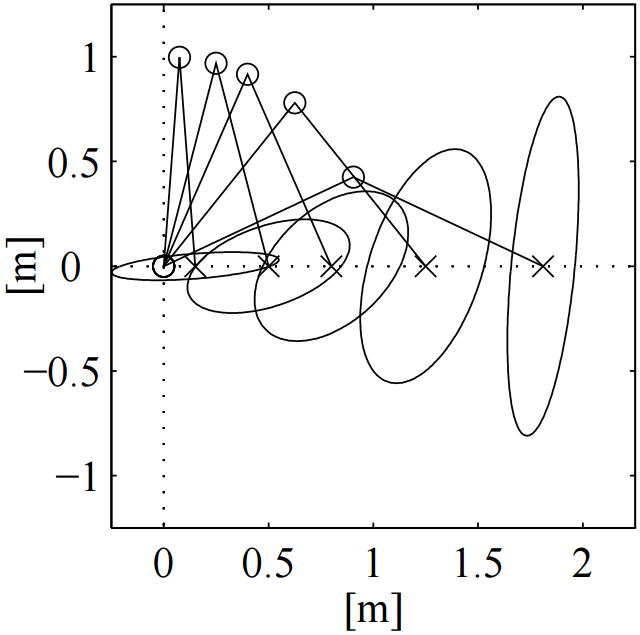
\includegraphics[width=1\textwidth]{Figura_3_23.png}
\end{minipage}

\newpage

%%%%%%%%%%%%%%%%%%%%%%%%%%%%%%%%%%%%%%%%%%%%%%%%%%%%%%%%%%%%%%%%%%%%%
\subsubsection{Indici Quantitativi di Manipolabilità}
Per permettere agli algoritmi di valutare numericamente una configurazione e di confrontarne diverse istante per istante è necessario condensare le informazioni della matrice $\bm{J}\bm{J}^T$ in valori scalari, detti \textit{indici di prestazione}.

\paragraph{Misura di Manipolabilità (Indice di Volume)}
L'indice più classico è la \textbf{misura di manipolabilità} $w(\bm{q})$. Geometricamente, questo scalare è proporzionale al \textbf{volume} dell'ellissoide di velocità. È definito come:
\[
    w(\bm{q}) = \sqrt{\det\left(\bm{J}(\bm{q})\bm{J}(\bm{q})^T\right)}
\]
Sfruttando le proprietà dell'algebra lineare, sappiamo che il determinante di una matrice è pari al prodotto dei suoi autovalori. Poiché gli autovalori di $\bm{J}\bm{J}^T$ sono i quadrati dei valori singolari $\sigma_i$ del Jacobiano, possiamo riscrivere l'indice come:
\[
    w(\bm{q}) = \sigma_1 \cdot \sigma_2 \cdot \dots \cdot \sigma_m
\]
Per un manipolatore non ridondante (dove $n=m$ e $\bm{J}$ è quadrata), questa espressione si semplifica ulteriormente in $w(\bm{q}) = |\det(\bm{J})|$.

\begin{itemize}
    \item Un valore elevato di $w$ indica che l'ellissoide ha un grande volume, suggerendo che il robot si trova in una configurazione "ben condizionata" dove può generare velocità con facilità.
    \item Se il robot raggiunge una singolarità, il valore singolare minimo $\sigma_{min}$ diventa nullo. Di conseguenza, il prodotto dei valori singolari si annulla: $w(\bm{q}) = 0$. Questo rende $w$ un ottimo indicatore per rilevare l'imminenza di una singolarità (il valore decresce rapidamente avvicinandosi ad essa).
\end{itemize}

Tuttavia, la misura di manipolabilità presenta due criticità:
\begin{enumerate}
    \item \textit{Dipendenza Dalla Scala:} L'indice non è adimensionale. Dipende dalle unità di misura e dalle dimensioni fisiche dei link. Un robot gigante avrà un $w$ molto più grande di un robot chirurgico, anche se la loro destrezza cinematica relativa fosse identica.
    \item \textit{Cecità Alla Forma:} Essendo un prodotto, $w$ non distingue tra un ellissoide sferico (buono) e uno molto schiacciato ma allungato (pessimo). Un ellissoide molto schiacciato può avere lo stesso volume di una sfera piccola, ma rappresenta una condizione vicina alla singolarità in certe direzioni.
\end{enumerate}

\paragraph{Numero di Condizionamento (Indice di Isotropia)}
Per ovviare ai problemi di scala e forma, si utilizza il \textbf{numero di condizionamento} della matrice Jacobiana, indicato con $\kappa(\bm{J})$. Esso è un indice adimensionale definito come il rapporto tra il massimo e il minimo valore singolare:
\[
    \kappa(\bm{J}) = \frac{\sigma_{\text{max}}}{\sigma_{\text{min}}} \quad \in [1, \infty)
\]
Geometricamente, questo valore rappresenta l'\textbf{eccentricità} dell'ellissoide, ovvero il rapporto tra la lunghezza dell'asse maggiore e quella dell'asse minore.
\begin{itemize}
    \item \textbf{Isotropia ($\kappa = 1$):} Si verifica quando $\sigma_{\text{max}} = \sigma_{\text{min}}$. L'ellissoide è una sfera perfetta. Il robot possiede la stessa capacità di movimento in tutte le direzioni. Questa è la configurazione ideale per la controllabilità uniforme.
    \item \textbf{Singolarità ($\kappa \to \infty$):} Quando ci si avvicina a una singolarità, $\sigma_{\text{min}}$ tende a zero, facendo esplodere il valore di $\kappa$. L'ellissoide diventa infinitamente schiacciato.
\end{itemize}
In sintesi, mentre $w$ misura "quanto" movimento globale si può generare, $\kappa$ misura l'\textbf{uniformità} di tale movimento. Nella progettazione di robot, si cerca spesso di mantenere $\kappa$ il più vicino possibile a 1 in tutto lo spazio di lavoro.
\newpage
\subsection{Ellissoide Di Manipolabilità In Forza}
Grazie alla dualità cineto-statica, si possono analizzare la capacità del robot di esercitare forze statiche sull'ambiente. Ricordiamo la relazione fondamentale della statica che lega le coppie ai giunti $\bm{\tau}$ alle forze cartesiane all'end-effector $\bm{f}$:
\[
    \bm{\tau} = \bm{J}^T(\bm{q}) \bm{f}
\]
Per costruire l'ellissoide di forza, si procede in modo analogo a quello di velocità. Immaginiamo di limitare le coppie dei giunti a una sfera unitaria (sforzo attuativo normalizzato):
\[
    \bm{\tau}^T\bm{\tau} \leq 1
\]
Sostituendo la relazione statica nell'equazione della sfera, si ottiene:
\[
    (\bm{J}^T\bm{f})^T (\bm{J}^T\bm{f}) = 1
\]
Sviluppando il prodotto trasposto ($\bm{A}\bm{B})^T = \bm{B}^T\bm{A}^T$, arriviamo all'equazione quadratica:
\begin{equation}
    \bm{f}^T \left( \bm{J}(\bm{q})\bm{J}(\bm{q})^T \right) \bm{f} = 1
\end{equation}
Questa equazione descrive l'\textbf{ellissoide di manipolabilità in forza}. Esso rappresenta le forze applicabili dall'end-effector dato uno sforzo unitario ai giunti.

\paragraph{Il Principio di Dualità Cineto-Statica.}
Confrontiamo le equazioni dei due ellissoidi per cogliere un aspetto fondamentale della meccanica robotica:
\begin{itemize}
    \item \textbf{Velocità:} $\bm{v}_e^T \left( \bm{J}\bm{J}^T \right)^{-1} \bm{v}_e = 1$
    \item \textbf{Forza:} $\quad \bm{f}^T \left( \bm{J}\bm{J}^T \right) \bm{f} = 1$
\end{itemize}
Notiamo che le matrici centrali delle forme quadratiche sono l'una l'inversa dell'altra.
Dalla teoria delle forme quadratiche $\bm{x}^T\bm{A}\bm{x}=1$, sappiamo che la lunghezza dei semiassi è data da $1/\sqrt{\lambda_i(\bm{A})}$.

Considerando la SVD, gli autovalori di $\bm{J}\bm{J}^T$ sono $\sigma_i^2$. Ne consegue che:
\begin{itemize}
    \item I semiassi dell'ellissoide di \textbf{velocità} hanno lunghezza $\sigma_i$.
    \item I semiassi dell'ellissoide di \textbf{forza} hanno lunghezza $1/\sigma_i$.
\end{itemize}
Questo risultato matematico formalizza il \textbf{Principio di Dualità}:
\begin{quote}
    \emph{Le direzioni in cui il robot ha la massima capacità di velocità (alto rapporto di trasmissione) sono esattamente quelle in cui ha la minima capacità di forza (basso vantaggio meccanico), e viceversa.}
\end{quote}

Questa dualità guida le strategie di pianificazione del compito:
\begin{itemize}
    \item Se il compito richiede \textbf{grandi velocità} (es. movimenti rapidi a vuoto), bisogna allineare la direzione del moto con l'asse maggiore dell'ellissoide di velocità ($\sigma_{max}$).
    \item Se il compito richiede l'applicazione di \textbf{grandi forze}, bisogna allineare la direzione della forza con l'asse maggiore dell'ellissoide di forza. Attenzione: questo corrisponde all'asse \textit{minore} dell'ellissoide di velocità ($\sigma_{min}$).
\end{itemize}
In pratica, un robot vicino a una singolarità ($\sigma_{min} \approx 0$) non può muoversi in quella direzione, ma paradossalmente è in grado di resistere a forze esterne enormi lungo quella stessa direzione senza affaticare i motori (si pensi a un braccio completamente disteso che regge un peso: lo sforzo è tutto sulla struttura meccanica, non sulla coppia dei giunti).


\newpage
\subsubsection{Esempio Applicativo: Il Compito Della Scrittura}

Per comprendere concretamente l'utilità degli ellissoidi, analizziamo un compito comune ma cinematicamente complesso: la scrittura su una superficie piana. Affinché un manipolatore (o il braccio umano) possa scrivere in modo efficace, deve soddisfare contemporaneamente due requisiti fisici contrastanti lungo direzioni ortogonali:

\begin{enumerate}
    \item \textbf{Direzione Verticale (Controllo di Forza):}
    Lungo l'asse $z$, perpendicolare al foglio, non è richiesto un movimento veloce, bensì la capacità di mantenere una pressione costante della penna sulla carta. È necessario compensare le irregolarità della superficie e l'attrito senza che la penna si stacchi o buchi il foglio.
    In termini di manipolabilità, ciò richiede che il robot sia in una configurazione in cui il vantaggio meccanico è massimo lungo la verticale. Pertanto, l'\textbf{ellissoide di manipolabilità in forza} deve avere il suo \textbf{asse maggiore orientato verticalmente}. Grazie al principio di dualità, questo implica che la capacità di velocità in questa direzione sarà minima, il che è accettabile poiché non dobbiamo muoverci verticalmente.

    \item \textbf{Direzione Orizzontale (Controllo di Velocità):}
    Sul piano $xy$ del foglio, il compito richiede di tracciare lettere e curve in modo fluido e rapido. Qui la forza richiesta è minima (solo quella necessaria a vincere l'attrito laterale), ma è fondamentale l'agilità cinematica.
    Di conseguenza, l'\textbf{ellissoide di manipolabilità in velocità} deve avere i suoi \textbf{assi maggiori giacenti sul piano orizzontale}. Ciò garantisce che piccole velocità ai giunti si traducano in ampi movimenti della penna, facilitando la scrittura.
\end{enumerate}

La configurazione ottimale per la scrittura è dunque quella che allinea gli assi principali degli ellissoidi con le direzioni naturali del compito (il cosiddetto \emph{Task Frame}).

È qui che entra in gioco la \textbf{ridondanza cinematica} (tipica del braccio umano a 7 gradi di libertà o dei robot collaborativi): un manipolatore ridondante può modificare la propria configurazione interna (i movimenti nel "null space") senza spostare la punta della penna, ruotando di fatto gli ellissoidi nello spazio fino a farli coincidere con le direzioni desiderate di forza e velocità.

\vspace{0.5cm}

\noindent
\begin{minipage}[c]{0.38\textwidth}
    \centering
    \resizebox{0.9\linewidth}{!}{%
        \begin{tikzpicture}
            % Piano di scrittura
            \draw[thick] (-2.5,0) -- (2.5,0) node[below right] {\small Piano di scrittura};

            % Penna stilizzata
            \draw[line width=1.5pt, fill=gray!30] (0,0.05) -- (0.2, 0.6) -- (-0.2, 0.6) -- cycle;
            \draw[thick, gray] (0, 0.6) -- (0, 2.3); % Asta penna/mano
            \node at (0,0) {$\bullet$};

            % Ellissoide di Forza (ROSSO) - Verticale
            % Indica alta capacità di forza verso il basso (pressione)
            \draw[red, thick, dashed] (0,0.8) ellipse (0.4cm and 1.2cm);
            \node[red, font=\footnotesize] at (1.1, 1.5) {Forza ($\bm{f}$)};
            % \draw[->, red] (0.5, 1.5) -- (0.1, 1.0);

            % Ellissoide di Velocità (BLU) - Orizzontale
            % Indica alta capacità di movimento laterale (scrittura)
            \draw[blue, thick, dashed] (0,0.8) ellipse (1.6cm and 0.5cm);
            \node[blue, font=\footnotesize] at (2.0, 0.25) {Velocità ($\bm{v}$)};
            % \draw[->, blue] (1.8, 0.6) -- (1.2, 0.8);

            % Assi cartesiani di riferimento locale
            \draw[->, thin] (-2, 2) -- (-1.5, 2) node[right] {$x$};
            \draw[->, thin] (-2, 2) -- (-2, 2.5) node[above] {$z$};
        \end{tikzpicture}
    }
\end{minipage}
\hfill
\begin{minipage}[c]{0.58\textwidth}
    \textbf{Interpretazione Grafica:}
    La figura mostra la configurazione ideale per la scrittura.
    \begin{itemize}
        \item L'\textcolor{blue}{ellissoide di velocità (blu)} è allungato orizzontalmente, indicando che il robot è "agile" nel tracciare le lettere sul piano.
        \item L'\textcolor{red}{ellissoide di forza (rosso)} è allungato verticalmente, indicando che il robot può esercitare o controllare efficacemente la pressione verso il basso.
    \end{itemize}
    Si noti la relazione di dualità: dove l'ellissoide blu è largo, quello rosso è stretto, e viceversa.
\end{minipage}

\vspace{0.5cm}

In conclusione, gli ellissoidi di manipolabilità trascendono il concetto di semplice indice numerico. Essi costituiscono uno strumento concettuale indispensabile per verificare la \textbf{compatibilità} tra la struttura cinematica del robot e i requisiti fisici del compito assegnato, guidando sia la progettazione meccanica che le strategie di controllo.

\end{document}
